
%%	Importiert die Rahmenbedingungen / importing all boundary conditions
\documentclass{scrreprt}		% Keine doppelte Überschrift bei chapters

\usepackage{geometry}			% Formatierung der Seitenränder
\geometry{
	a4paper, 
	top=20mm, 
	left=20mm, 
	right=20mm, 
	bottom=20mm, 
	headsep=10mm, 
	footskip=12mm
}

\usepackage[utf8]{inputenc}		% Ermöglicht nahezu alle Zeichencharakter ohne sonderzeichen Kennzeichnung
\usepackage[ngerman]{babel}
\usepackage[utf8]{inputenc}
\usepackage[nottoc]{tocbibind}
\usepackage{textcomp}
\usepackage{xcolor} 			% Ermöglichen von verschiedenen Farben z. B. Hyperlinks
\usepackage{color} 
\usepackage{colortbl}
\usepackage{makecell}

% Einrichten von Hyperlins innerhalb des PDF Dokuments
\usepackage[
	pdfpagelabels, 
	bookmarksopen=true, 
	bookmarksnumbered=true, 
	linkcolor=black, 
	hypertexnames=false
] {hyperref} 

\usepackage{graphicx}			% Einbinden von Grafiken

\usepackage[final]{pdfpages}
\usepackage{array}
\usepackage{upgreek}
\usepackage{amsmath}			% Mathematische Funktionalitäten
\usepackage{amssymb}			% Mathematische Symbole
\usepackage{amsfonts}
\usepackage{leftidx}
\usepackage{caption,pdfpages}

\usepackage{capt-of}			% Überschriften bei minipages

\usepackage{wrapfig}			% Text um Grafik wrappen
\usepackage{subcaption}

\usepackage{booktabs}
\usepackage{tabularx}

\usepackage{url}

\usepackage[footnote,nohyperlinks]{acronym}	% Ermöglicht das Abkürzungsverzeichnis, darstellung der langform als footnote
% --- Weitere Optionen --- %
% footnote 		-- 	die Langform als Fußnote ausgeben
% nohyperlinks 	-- 	wenn hyperref geladen ist, wird die Verlinkung unterbunden
% printonlyused -- 	nur Abkürzungen auflisten, die tatsächlich verwendet werden.
						% Im printonlyused-Modus kann zusätzlich noch die Option withpage verwendet werden. Hierdurch wird im Abkürzungsverzeichnis zusätzlich die Seitenzahl, auf welcher die Abkürzung als erstes verwendet wurde, ausgegeben.
% smaller 		-- 	Text soll kleiner erscheinen, das Paket relsize wird vorausgesetzt
% dua 			-- 	es wird immer die Langform ausgegeben
% nolist 		-- 	es wird keine Liste mit allen Abkürzungen ausgegeben
% --- % Referenz: https://de.wikibooks.org/wiki/LaTeX-Wörterbuch:_Abkürzungsverzeichnis %% Stand 12.08.15

\setlength{\parindent}{0pt}	% Entfernen von automatischen Texteinrückungen nach einem Absatz



\begin{document}

%####################################################################%
	%%	Deckblatt / Topsheet
%####################################################################%

	%%	Bindet das Deckblatt ein / Import cover sheet
	\begin{titlepage}
\thispagestyle{empty}

\begin{center}
	\enlargethispage{3\baselineskip}
	\hrule
	
	\begin{center} \LARGE \textbf{\\Szenenekonstruktion und Kamerakalibrierung aus stereoskopischen Bildquellen gleicher und verschiedener Auflösungen}
	\end{center}
	
%	Stereokalibrierung und Szenenrekonstruktion aus heterogenen Bildquellen in Bezug auf Kameras gleicher und unterschiedlicher Auflösungen
	\vspace{0.5cm}
	
	\hrule
	
	\vspace{2.5cm}
	
	{\Large \textbf{Thesis}\\ zur Erlangung des Grades\\[2ex]
	\textbf{Master of Science}}
	
	\vspace{3cm}
	
	\begin{tabular}{l l l l}
		Medieninformatik &4.Semester &Anja Kretschmer &254793 \vspace{0.2cm} \\	
	\end{tabular}
	
	\vspace{1cm}
	
	\begin{align*}
	\text{Betreut von: }  &\text{Prof. Dr. Thomas Schneider}\\
	\end{align*}	
	
	\vspace{1.0cm}
	
%	Disclaim here
	
	\vspace{1.5cm}
	
\includegraphics[width=0.5\textwidth]{./images/hfu_logo.png}

	Fakultät Digitale Medien der Hochschule Furtwangen\\[1ex]
	Wintersemeter 17/18 - Sommersemeter 18

\end{center}

\end{titlepage}
	
	%%	Erzwingt eine neue Seite / Force new page
	\newpage
	
%####################################################################%
	%%	Inhaltsverzeichnis / Table of contents
%####################################################################%

	%%	Erstellt das Inhaltsverzeichnis / Generate the index
	\tableofcontents
	
	%%	Erzwingt eine neue Seite / Force new page
	\newpage
	
%####################################################################%
	%% Inhalt / Content
%####################################################################%
	\addchap{Abstract}
 
 Over the last decades computer vision scientist have taken a new approach to vision. They build different computational models of what shoud be computed, what can really be computed, and how these computations can be realized by computer programs, and they use computers to test their models are correct. The result is a better understandung of vision from a different point of view, and at the same time some working artificial vision systems are built that can be used in idustry, medicine, etc. The knowledge obtained on neirophysiology and psychophysics have given hints to and influenced computer vision scientists, helping find solutions to the design of specific algorithms and implementation of vision systems. On the other Hand coputational vision has also given nerophysiologists and psychophysicsist a mathematical framework for modeling vision processes.\cite{ZZGXr}
 
 
 Abstract: wichtigkeit/aktualität von szenenrekonstruktion...  In dieser arbeit wurde ein szenenenrekonstruktionsalgorithnus implementiert und getestet... der implemtierte algorithmus wurde implementiert um bilder verschiedene Kamera-Auflösung zu rekonstruieren...
 Ergebniss: algorithmus funktionier, mit einigen problemen, wobei erste lösungsvorschläge aufgezeigt werden
	% Bindet die Einleitung ein / Import introducing
	\chapter{Einleitung}
\label{sec:einleitung} 

Hier auch erwähnen in welchem Kameramodell wir uns befinden (LITERATUR FINDEN DIE NICHT HZ IST!!)\\
Generelle kleine einleitung über kamerakalibrierung und was das genau ist (NICHT VIEL!!)

Kameramodellbeschreibung geometrisch in \cite{Jianzhong}\\

Ziel ist es auch bestimmte unklarheiten in der Literatur wie Einheiten in rechnungen wie fundamental und essentielle matrix aus der welt zu schaffen.\\

expliziet darauf eingehen, was es bedeutet zwei gleiche und zwei unterschiedliche Resolutions der Kameras zu besitzen gerade in Bezug auf die Ermittlung von F und E und der Szenenrekonstruktion(LITERATUR FINDEN DIE NICHT HZ IST!!)\\

Erwähnen mit was alles gearbeitet wurde (mathematica, Geogebra, Matlab, Unity(nur wenig))


	\begin{minipage}{\linewidth}
	\centering
	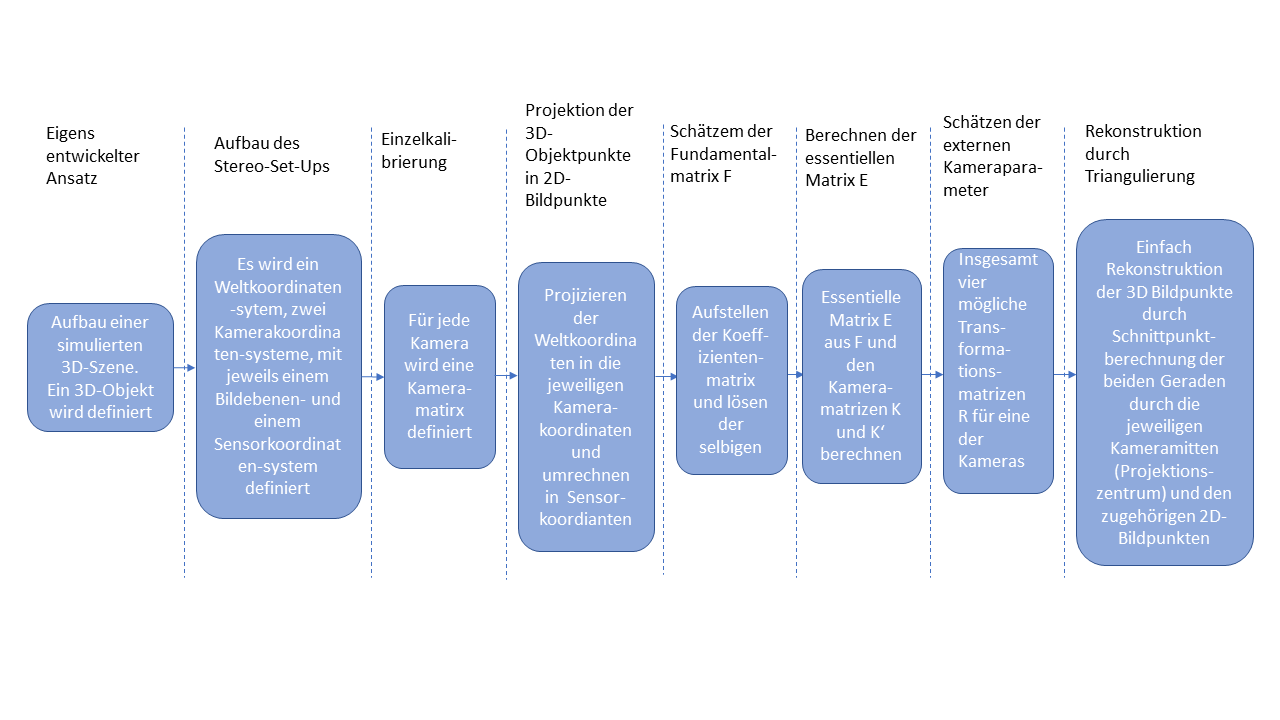
\includegraphics[width=1.\linewidth]{images/ArbeitsProzessMinimal.png}
	\captionof{figure}{Arbeitsprozesse der Stereoanalyse bei Verwendung von eigens erstellten synthetischen Bilddaten}
\end{minipage}\\ \\


	\begin{minipage}{\linewidth}
	\centering
	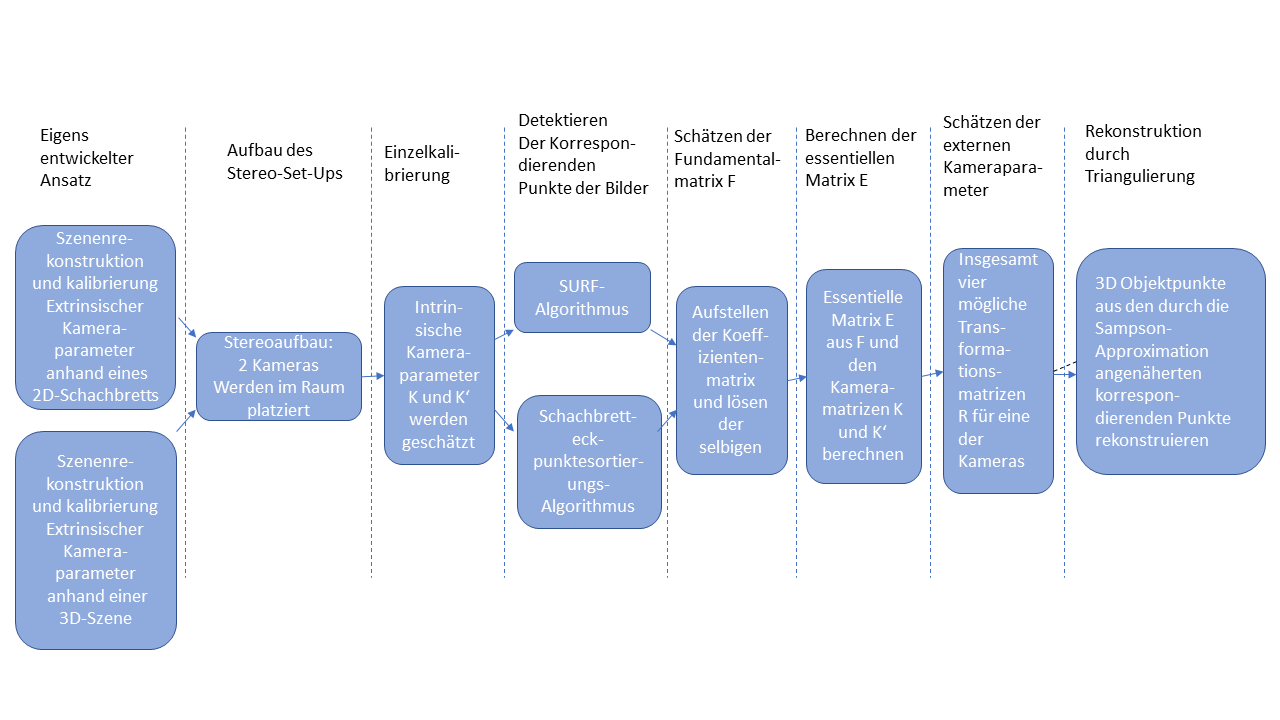
\includegraphics[width=1.\linewidth]{images/ArbeitsProzessReal.png}
	\captionof{figure}{Arbeitsprozesse der Stereoanalyse bei Verwendung von realen Bilddaten}
\end{minipage}\\ \\

\nameref{sec:einleitung}

%--------------------------------------------------------------------%
		%% Eigener Inhalt / Own content
%--------------------------------------------------------------------%
		
		%------------------------------------------------------------%
			%% Kapitel 1 / Chapter 1 (C1)
		%------------------------------------------------------------%
		\chapter{Kameramodelle}
\label{sec:CameraModels}



Kameramodellbeschreibung geometrisch in \cite{Jianzhong}\\


Simply put, a computational model for
a camera, at least for its geometric part, tells how to project 3D entities
(points, lines, etc.) onto the image, and vice versa, how to back-project
from the image to 3D.\cite{CamerModels.}\\

One of the principal topics of this book is the process of image formation, namely the
formation of a two-dimensional representation of a three-dimensional world, and what
we may deduce about the 3D structure of what appears in the images.
The drop from three-dimensional world to a two-dimensional image is a projection
process in which we lose one dimension. The usual way of modelling this process is
by central projection in which a ray from a point in space is drawn from a 3D world
point through a fixed point in space, the centre of projection.\cite{HZ}\\

This ray will intersect a
specific plane in space chosen as the image plane. The intersection of the ray with the
image plane represents the image of the point. If the 3D structure lies on a plane then
there is no drop in dimension.
This model is in accord with a simple model of a camera, in which a ray of light
from a point in the world passes through the lens of a camera and impinges on a film or
digital device, producing an image of the point. Ignoring such effects as focus and lens
thickness, a reasonable approximation is that all the rays pass through a single point,
the centre of the lens.\cite{HZ}

Kameras werden als Punkte dargestellt(Projektionszentren)

(GRAFIK EINFÜGEN SIEHE HZ SEITE 8)

Cameramodels:
\begin{itemize}
	\item Global Camera models : Pinhole Camera
	\item local Camera models
	\item discrete Camera models
\end{itemize}


Most models
have a single optical center through which all camera rays pass. We
also speak of central camera models.For these, the back-projection
function (see below) delivers the direction of the camera ray. Noncentral
camera models do not possess a single optical center. In
that case, the back-projection operation has to deliver not only the
direction but also the position of a camera ray, e.g., some finite point
on the ray.\cite{CamerModels.}

By “classical models”, we mean those used most often in applications
and academic research, i.e., the pinhole model, affine camera models,
and pinhole models enhanced with classical terms for radial and tangential
distortions.\cite{CamerModels.}\\

	\begin{gather}
K=\begin{bmatrix}
\alpha_x&s&x_{0}\\
0&\alpha_y&y_{0}\\
0&0&1
\end{bmatrix}
\end{gather}\\

we will assume square pixels, i.e., s = 0 and fu=fv=f. Mehr dazu im Kapitel \nameref{sec:basisTransformation}

	\begin{minipage}{\linewidth}
	\centering
	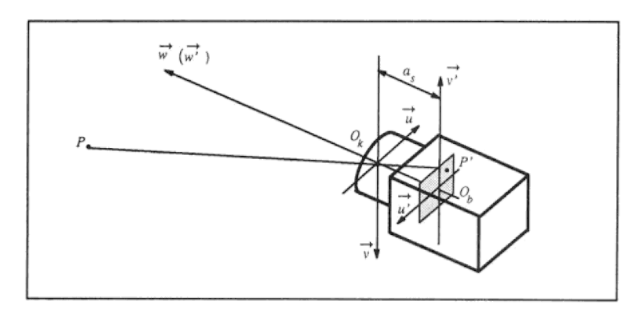
\includegraphics[width=.8\linewidth]{images/kameramodell_vorlaeufig.png}
	\captionof{figure}{Lochkameramodell \cite{Jianzhong}}
	\label{fig:PinholeCamera}
\end{minipage}\\ \\

Koordinatensysteme des Pinhole models erklären: insgesamt werden 5 benötigt um einen 3D punkt auf einen Bildpunkt zu transformieren, mehr dazu im Kapitel \nameref{sec:basisTransformation}

Reconstruction from more than one view:The simplest case is that of two images, which we will consider
first. As a mathematical abstraction, we restrict the discussion to “scenes” consisting of points only.
The usual input to many of the algorithms given in this book is a set of point correspondences.
In the two-view case, therefore, we consider a set of correspondences $x_i \Leftrightarrow x'_i$ in two images.

It is assumed that there exist some camera matrices, $P$ and $P'$ and a set of 3D points $X_i$ that give rise to these image correspondences in the sense that $PX_i = x_i$ and $P'_iX_i = x'_i$. Thus, the point $X_i$ projects to the two given data points. However, neither the cameras (represented by projection matrices $P$ and $P'$), nor the points $X_i$ are known. It is our task to determine them.\\




	Um die Kameramatrix allgemeiner zu formulieren und die Bedeutung und hinter $\zeta$ und dessen Zusammenhang mit dem in der Literatur benutzten $f$ genauer zu erläutern, wird die Kameramatrix der Photogrammetrie in Bezug auf ein Lochkameramodell hier noch einmal genauer betrachtet und mit dem hergeleiteten Modell verglichen\cite{HZ,Heipke}. Zur Beschreibung optischer Kameras greift man üblicherweise auf das Lochkameramodell zurück. Das Modell beruht ausschließlich auf der geometrischen Optik und vernachlässigt physikalische Effekte wie Beugung oder die Auswirkungen der Linse \cite{Heipke}.  Nehmen wir an es gilt $\zeta = f$, dann gilt für die Projektion von Punkten das selbe wie in Gleichung 2.49 nur mit $f$ statt $\zeta$. 

\begin{gather}
\begin{bmatrix}
X\\Y\\Z\\1
\end{bmatrix} \mapsto
\begin{pmatrix}
\zeta X\\ \zeta Y\\ Z
\end{pmatrix}
=
\begin{bmatrix}
\zeta&0&0&0\\
0&\zeta&0&0\\
0&0&1&0
\end{bmatrix}
\cdot
\begin{bmatrix}
X\\Y\\Z\\1
\end{bmatrix}
=
\begin{pmatrix}
\zeta \frac{X}{Z}\\ \zeta \frac{Y}{Z}\\1
\end{pmatrix}\\
\leadsto
\begin{bmatrix}
X\\Y\\Z\\1
\end{bmatrix} \mapsto
\begin{pmatrix}
f X\\ f Y\\ Z
\end{pmatrix}
=
\begin{bmatrix}
f&0&0&0\\
0&f&0&0\\
0&0&1&0
\end{bmatrix}
\cdot
\begin{bmatrix}
X\\Y\\Z\\1
\end{bmatrix}
=
\begin{pmatrix}
f \frac{X}{Z}\\ f \frac{Y}{Z}\\1
\end{pmatrix}
\end{gather}

Zum Vergleich dient die Definition im Buch von \textit{Hartley \& Zisserman}\cite{HZ}, welche der selbst hergeleiteten entspricht.


\begin{gather}
\begin{bmatrix}
X\\Y\\Z\\1
\end{bmatrix} \mapsto
\begin{pmatrix}
f X\\ f Y\\ Z
\end{pmatrix}
=
\begin{bmatrix}
f&0&0&0\\
0&f&0&0\\
0&0&1&0
\end{bmatrix}
\cdot
\begin{bmatrix}
X\\Y\\Z\\1
\end{bmatrix}
\end{gather}		


Die Kameramatrix $K$ lautet in der Literatur\cite{HZ}:

\begin{gather}
K=\begin{bmatrix}
\alpha_x&s&x_{0}\\
0&\alpha_y&y_{0}\\
0&0&1
\end{bmatrix}
\end{gather}

Anstelle von $f$ steht in der Kameramatrix aus Gleichung 2.42 $\alpha_x$ und $\alpha_y$. Die Werte welche $\alpha_x$ und $\alpha_y$ annehmen können, hängen von der geometrischen Form der Pixel des in der Kamera verbauten Sensors ab\cite{HZ,Photonik}.  $\alpha_x$ und $\alpha_y$ sind genau dann einheitlich, wenn die Form der verbauten Pixel, ebenfalls einheitlich quadratisch ist. Die Einheiten der x- und y- Achsen des Sensorkoordinatensystems sind einheitlich. $\alpha_x$ und $\alpha_y$ sind also genau dann ungleich, wenn die auf dem Sensor verbauten Pixel beispielsweise rechteckig oder die geometrische Form eines Parallelogramms besitzen\cite{HZ}. Im Stereoaufbau dieser Arbeit, wurden Kameras mit CMOS-Chips mit quadratischen Pixeln verwendet, weshalb $\alpha_x$ und $\alpha_y$ einheitlich sein werden. $\alpha_x$ und $\alpha_y$ entstehen aus der Multiplikation der Werte für $\zeta_x$ und $\zeta_y$ beziehungsweise  $f_x$ und $f_y$ mit einem jeweiligen Skalierungswert $m_x$ und $m_y$. Sind die Pixel nicht quadratisch, wird auf die Werte $f_x$ und $f_y$ jeweils eine Skalierung $m_x$ und $m_y$ drauf multipliziert so dass  $\alpha_x = f_x \cdot m_x$ und $\alpha_y = f_y \cdot m_y$ entspricht\cite{HZ}. Die Matrixeinträge,$x_{0}$ und $y_{0}$, bilden einen Translationsvektor. Sie beinhalten die Position des Hauptpunkts auf der Bildebene. $x_{0}$ und $y_{0}$ sind definiert als $x_{0} = p_x \cdot m_x$ und $x_{0} = p_y \cdot m_y$. Der Matrixeintrag $s$ wird dem sogenannten \textit{skew-Faktor} zugeordnet, welcher nur dann zum Einsatz kommt, sollte die optische Achse nicht orthogonal auf den Bildsensor auftreffen. Sprich wenn der Chip geneigt in der Kamera montiert wurde\cite{HZ}. Die komplette Projektionsmatrix $P=KR=K[C|v]$ beziehungsweise wie sie in der Literatur zitiert wird $P=K[R|t]$\cite{HZ} besteht aus der Matrixmultiplikation der hergeleiteten Transformationsmatrix $R$ welche die externen Kamerparameter repräsentiert und der Kameramatrix $K$, welche die internen Kameraparameter repräsentiert. $P$ beinhaltet also sowohl die internen als auch die externen Kameraparameter.

\subsection{Kameraparameter}

internen externe parameter\cite{Jianzhong}

Pinhole model. The pinhole model, or perspective projection,
assumes that all camera rays pass through a single point, the optical
center and that there is a linear relationship between image point
position and the direction of the associated camera ray. That relationship
can be expressed via a so-called calibration matrix which depends
on up to five intrinsic parameters:\cite{CamerModels.}\\



Basis Transformationen um Objektpuntke aus sicht der verschiedenen Koordiantensysteme beschreiben zu können \\
Geometrien kurz einführen: benötigte Geometrien sind Homographien, um mit Punkte auf der bildebene zu hantieren \\
Epipolargeometry um geometrische Bezihungen zwischen Bildpunkten, Objektpunkt etx herzustellen
		% C1 - example 1
		%\chapter{Koordinatensysteme im Lochkamermodell}
\label{sec:basisTransformation} 

(Neue Einleitung schreiben)
 
In diesem Kapitel wird der Fokus auf die benötigten Koordinatensysteme für die Stereobildanalyse gelegt. Als aller erstes werden anhand praxisnaher Beispiele die Notwendigkeit der Basis Transformation und damit einhergehend der Spezialfall einer Transformation von einem Koordinatensystem wie zum Beispiel einem dreidimensionalen Weltkoordinatensystem $(O,\delta)$ mit $\delta=(\hat{d_1}, \hat{d_2},\hat{d_3},O)$ in ein dreidimensionales Kamerakoordinatensystem $(C,\beta)$ mit $\beta=(\hat{b_1},\hat{b_2},\hat{b_3},C)$ aufgezeigt. Die gewählte Notation zur Beschreibung der Koordinatensysteme setzt sich am Beispiel des Kamerakoordinatensystem aus der Bezeichnung für den Ursprung $C$ und den entsprechenden Koordinatenachsen $(\hat{b_1},\hat{b_2},\hat{b_3})$ mit wiederum $\hat{b_1} = \begin{pmatrix}b_{11}\\b_{12}\\b_{13}\end{pmatrix}$, $\hat{b_2} = \begin{pmatrix}b_{21}\\b_{22}\\b_{23}\end{pmatrix}$ und $\hat{b_1} = \begin{pmatrix}b_{31}\\b_{32}\\b_{33}\end{pmatrix}$, welche mit $\beta$ zusammengefasst werden. In Abbildung \ref{fig:Koordinatensysteme1} sind die beiden kartesischen Koordinatensysteme $(O,\delta)$ und $(C,\beta)$ schematisch dargestellt. 

% werden zunächst ein paar Grundlegende mathematische Operationen vorgestellt, welche das Grundgerüst der Stereokalibrierung und Szenenrekonstruktion bilden.
%
%Noch anzumerken ist, dass in dieser Arbeit grundlegend von orthogonalen Koordinatensystemen ausgegangen wird, andernfalls wird explizit darauf hingewiesen. 
%
%

%\section{Die Transformation von Koordinaten schließt die Transformation der Basis mit ein}
%
%Es sei \textit{V} ein \textit{n}-Dimensionaler Vektorraum über einem Körper \textit{K}. \textit{K} stellt in diesem Beispiel das Skalar \ensuremath{\mathbb{R}} dar, welches alle reelen Zahlen mit einschließt. Zur Veranschaulichung wird der Vektorraum  \ensuremath{V^3} also ein 3-Dimesnionaler Raum gewählt, dessen Basis mit \ensuremath{\beta = [\vec{b}_1, \vec{b}_3, \vec{b}_3]} bezeichnet wird.\cite{Elements} ....  (FORTFÜHREN)\\
%
%A vector $\vec{v} \in V^3$ is uniquely expressed as a linear combination of basic vectors of V 3 by its coordinates $(x,y,z) \in \mathbb{R}$. $\vec{v} = xb_1+yb_2+zb_3$ and can be represented as an ordered triple of coordinates, $\vec{v}_\beta =[x\,y\,z]^T$

\section{Koordinatentransformation durch Basistransformationen}

Anhand eines Beispiels wird im folgenden eine Transformation eines Punktes bezüglich des Weltkoordinatensystems in das Kamerakoordinatensystem veranschaulicht. Es soll in einer Symbolischen Schreibweise Punkte aus einem Weltkoordinatensystem  
$(O,\delta)$ mit $\delta = (\hat{d_1},\hat{d_2},\hat{d_3})$ in ein Kamerakoordinatensystem  $(C,\beta)$ mit $\beta = (\hat{b_1},\hat{b_2},\hat{b_3})$ überführt werden, dessen Ursprung eine Verschiebung und Rotation zum Weltkoordinatensystem aufweist. Beispielhaft wird dies in Abbildung \ref{fig:Koordinatensysteme1} aufgezeigt.
 
	\begin{minipage}{\linewidth}
		\centering
		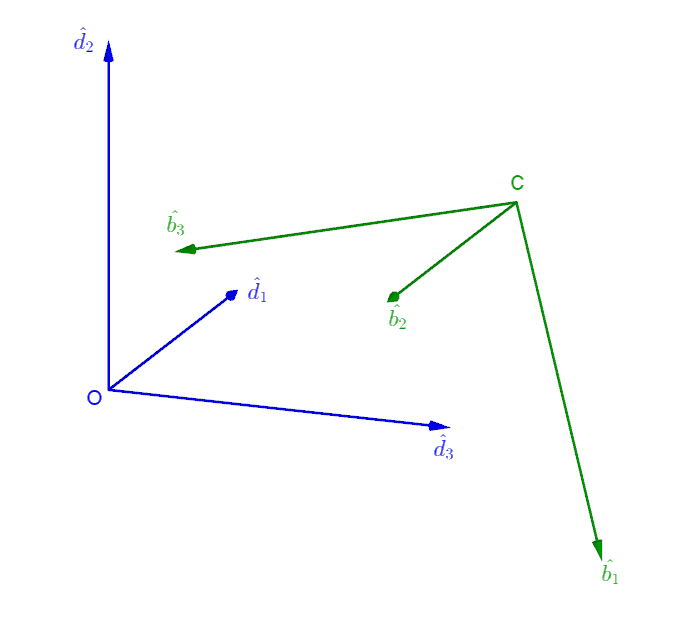
\includegraphics[width=0.7\linewidth]{images/WeltKordSys.png}
		\captionof{figure}{Weltkoordinatensystem $(O,\delta)$ mit $\delta = (\hat{d_1},\hat{d_2},\hat{d_3})$ und Kamerakoordinatensystem  $(C,\beta)$ mit $\beta = (\hat{b_1},\hat{b_2},\hat{b_3})$ }
		\label{fig:Koordinatensysteme1}
	\end{minipage}\\ \\
	
	
Zunächst wird eine sogenannte Koordinatisierung von Punkten im Weltkoordinatensystem vorgenommen. Ein Punkt $P_\delta$ bezüglich des Weltkoordinatensystems wird dann wie folgt beschrieben.

	
	\begin{gather}
	P_\delta = O + p_{1\delta}\hat{d_1} + p_{2\delta}\hat{d_2} + p_{3\delta}\hat{d_3}\\
	\leadsto P_\delta = (p_{1\delta},p_{2\delta},p_{3\delta})^T = \begin{pmatrix} p_{1\delta} \\ p_{2\delta} \\ p_{3\delta} \end{pmatrix}
	\end{gather}
	
Um das Koordinatentupel in einem projektiven Raum darstellen zu können, wird es projektiv erweitert. Die Entstehenden projektiv erweiterten Koordinaten werden als homogene Koordinaten bezeichnet. Ein Punkt $P_\delta$ bezüglich des Weltkoordinatensystems wird um eine vierte homogene Komponente erweitert. Diese kann einen Wert zwischen 0 und 1 annehmen. Nimmt die Komponente den Wert 0 an, so handelt es sich um einen Fernpunkt, sprich der Punkt liegt im unendlichen.
%wird dann zum Zweck der Einführung homogener Objekte projektiv Erweitert.
	
	\begin{gather}
	P_\delta = \begin{bmatrix} p_{1\delta} \\ p_{2\delta} \\ p_{3\delta} \\1 \end{bmatrix} = \left\{ k \begin{bmatrix} p_{1\delta}\\p_{2\delta}\\p_{3\delta}\\1 \end{bmatrix} \in \mathbb{R} ^4 |  k \in \mathbb{R}\right\}\\
	\begin{bmatrix}\lambda p_{1\delta}\\ \lambda p_{2\delta} \\ \lambda p_{3\delta} \\ 1 \end{bmatrix} = \begin{bmatrix}p_{1\delta} \\ p_{2\delta} \\ p_{3\delta} \\ 1\end{bmatrix} \text{für} \; \lambda \ne 0
	\end{gather}


Ein Punkt $P_\beta$ bezüglich des Kamerakoordinatensystem wird im Vergleich wie folgt beschrieben.
	
	\begin{gather}
	P_\beta = C + p_{1\beta}\hat{b_1} + p_{2\beta}\hat{b_2} +  p_{3\beta}\hat{b_3}\\
	P_\beta = \begin{pmatrix} p_{1\beta} \\  p_{2\beta} \\ p_{2\beta}\end{pmatrix}
	\end{gather}\\
	
	Zwischen den beiden Koordinatensystemen	$(O,\delta)$  und $(C,\beta)$ werden die folgenden Beziehungsgleichungen aufgestellt. 
	
	\begin{gather}
	C_\beta = O_\delta + C_{\beta,1}\hat{d_1} +C_{\beta,2}\hat{d_2} + C_{\beta,3}\hat{d_3}\\
	\hat{b_1} = b_{11}\hat{d_1} +  b_{12}\hat{d_2} +  b_{13}\hat{d_3}\\
	\hat{b_2} = b_{21}\hat{d_1} +  b_{22}\hat{d_2} +  b_{23}\hat{d_3}\\
	\hat{b_3} = b_{31}\hat{d_1} +  b_{32}\hat{d_2} +  b_{33}\hat{d_3}
	\end{gather}
	
	Diese Beziehungsgleichungen werden in Gleichung 3.1 eingesetzt.
	
	\begin{gather}
	\begin{split}
	P_\delta = O + (C_{\beta,1} + p_{1\beta}b_{11} +  p_{2\beta}b_{21} + p_{3\beta}b_{31}) \cdot \hat{d_1}\\
	+(C_{\beta,2} + p_{1\beta}b_{21} +  p_{2\beta}b_{22} + p_{3\beta}b_{32} )\cdot \hat{d_2}\\
	+ (C_{\beta,3} + p_{1\beta}b_{31} +  p_{2\beta}b_{23} + p_{3\beta}b_{33} )\cdot \hat{d_3}
	\end{split}
	\end{gather}
	
Aus Gleichung 3.11 wird ein Gleichungssystem in der Form von Gleichung 3.12 aufgestellt und gelöst.
	
	\begin{gather}
	\begin{split}
	p_{1\delta} = C_{\beta,1} + (C_{\beta,1} + p_{1\beta}b_{11} +  p_{2\beta}b_{21} + p_{3\beta}b_{31} \\
	\leadsto \: p_{1\delta} - C_{\beta,1} =  (C_{\beta,1} + p_{1\beta}b_{11} +  p_{2\beta}b_{21} + p_{3\beta}b_{31})
	\end{split}
	\end{gather}
	
Wenn $P_\beta$ gegeben ist, erhält man auf diese Weise direkt $P_\delta$. Wenn jedoch  $P_\delta$  gegeben ist, so muss das in Gleichung 3.13 aufgestellte lineare Gleichungssystem gelöst werden.
	
	\begin{gather}
	\begin{bmatrix}b_{11} & b_{21} & b_{31}\\
	b_{12} & b_{22} & b_{32}\\
	b_{13} & b_{23} & b_{33}
	\end{bmatrix} 
	\begin{pmatrix}
	p_{1\beta}\\p_{2\beta}\\ p_{3\beta}
	\end{pmatrix} = 
	\begin{pmatrix}
	p_{1\delta} - C_{\beta,1}\\
	p_{2\delta} - C_{\beta,2}\\
	p_{3\delta} - C_{\beta,3}
	\end{pmatrix}
	\end{gather}
	
 Wenn $(C,\beta)$ ein kartesisches Koordinatensystem ist, so ist die entstehende  koeffizientenmatrix $D_\beta$ orthogonal und es gilt \ensuremath{D_\beta^{-1} = D_\beta^T}. 
	\begin{gather}
	D_\beta^{T} = 
	\begin{bmatrix}b_{11} & b_{12} & b_{13}\\
	b_{21} & b_{22} & b_{23}\\
	b_{31} & b_{32} & b_{33}
	\end{bmatrix} \\
	\begin{split}
	\leadsto \: \begin{pmatrix}
	p_{1\beta}\\p_{2\beta}\\ p_{3\beta}
	\end{pmatrix}
	= D_\beta^T 
	\begin{pmatrix}
	p_{1\delta} - C_{\beta,1}\\
	p_{2\delta} - C_{\beta,2}\\
	p_{3\delta} - C_{\beta,3}
	\end{pmatrix}
	\end{split} 
	\end{gather}
	
Handelt es sich um kein kartesisches Koordinatensystem, so muss lediglich die Inverse \ensuremath{D_\beta^{-1}} anstatt der Transponierten \ensuremath{D_\beta^T} gebildet und wie gehabt verfahren werden. Im folgenden wird noch einmal kompakt und in einer symbolischen Schreibweise die Transformation von Welt- in Kamerakoordinaten  festgehalten. Einmal wird wie bereits angefangen mit Spaltenvektoren gearbeitet, das selbe Verfahren wird dann noch einmal mit Zeilenvektoren dargestellt.  Beide Ansätze funktionieren nach dem selben Prinzip, der einzige Unterschied ist die Darstellung der Matrizen. Es ist jedoch gerade wenn man mit Programmen wie Beispielsweise \textit{Matlab} arbeitet wichtig zu wissen welche Darstellung benutzt wird und worin sie sich unterscheiden. Auf diese weise passieren keine Fehler beim Interpretieren der späteren Resultate. \textit{MatLab} arbeitet beispielsweise mit Spaltenvektoren, während im entstandenen Algorithmus dieser Arbeit mit Zeilenvektoren gearbeitet wurde. Zunächst wird also weiter mit Spaltenvektoren verfahren. Zur Erinnerung, es gilt, dass $\beta = (\hat{b_1},\hat{b_2},\hat{b_3},C)$ durch Rotation $D$ aus $\delta = (\hat{d_1},\hat{d_2},\hat{d_3})$ entstanden ist. Der Ursprung des Kamerakoordinatensystems ist bezüglich des Ursprungs des Weltkoordiantensystems verschoben. Zur Rotation des Koordinatesystems muss also auch noch eine Tranlation des Ursprungs durchgeführt werden. Der Translationsvektor ist gleich den Koordinaten des Ursprungs des Kamerakoordinatensystem $\vec{V} = C_\beta = (C_{\beta,1}, C_{\beta,2}, C_{\beta,3})^T$. Die Transformationsmatrix welche aus der Rotation $D$ und dem Translationsvektor $\vec{V}$ ensteht, wird im weiteren Verlauf mit $R$ bezeichnet.

%Da es sich aber in einem nicht-kartesischen Koordinatensystem nicht um eine orthogonale Drehmatrix handelt wird die Rotation \textit{R} in diesem Beispiel als Transformationsmatrix \textit{C} gekennzeichnet.
% Somit soll gekennzeichnet werden, dass die Transformation unabhängig der Definition ihres ausgehenden Koordinatensystem allgemein formuliert werden kann. Es gilt für die Transformation von Welt- in Kamerakoordinaten ausgehend von Spaltenvektoren folgendes.
	
	\begin{gather}
	\begin{pmatrix}
	\hat{b_1}\\
	\hat{b_2}\\
	\hat{b_3}\\
	C_\beta
	\end{pmatrix} = 
	\begin{bmatrix}
	b_{11} & b_{21} & b_{31} & 0\\
	b_{12} & b_{22} & b_{32} & 0\\
	b_{13} & b_{23} & b_{33} & 0\\
	C_{\beta,1} & C_{\beta,2} & C_{\beta,3} & 1
	\end{bmatrix}
	\begin{pmatrix}
	\hat{d_1}\\
	\hat{d_2}\\
	\hat{d_3}\\
	O_\delta
	\end{pmatrix}\\
	D^T = D^{-1}= \begin{bmatrix}
	b_{11} & b_{12} & b_{13} \\
	b_{21} & b_{22} & b_{23} \\
	b_{31} & b_{32} & b_{33} 
	\end{bmatrix}\\
	D = \begin{bmatrix}
	b_{11} & b_{21} & b_{31} \\
	b_{12} & b_{22} & b_{32} \\
	b_{13} & b_{23} & b_{33} 
	\end{bmatrix}
	\end{gather}

Für eine Rücktransformation von Kamera in Weltkoordinaten muss die Inverse von $D$ gebildet werden.
Außerdem muss der Translationsvektor $\vec{V}$ ebenfalls mit dieser Inversen multipliziert werden, um diesen ebenfalls in das Zielkoordinatensystem zu überführen.
	
	
	\begin{gather}
	\leadsto \: \begin{pmatrix}
	\hat{d_1}\\
	\hat{d_2}\\
	\hat{d_3}\\
	O_\delta
	\end{pmatrix} = 
	\begin{bmatrix}
	b_{11} & b_{21} & b_{31} & 0\\
	b_{12} & b_{22} & b_{32} & 0\\
	b_{13} & b_{23} & b_{33} & 0\\
	&-(	C_{\beta,1}, C_{\beta,2}, C_{\beta,3})C^{-1}& & 1
	\end{bmatrix}
	\begin{pmatrix}
	\hat{b_1}\\
	\hat{b_2}\\
	\hat{b_3}\\
	C_\beta
	\end{pmatrix}
	\end{gather}
	
	
Das selbe Verfahren mit Zeilenvektoren führt zu den Gleichungen 3.20 und 3.21.
	
%	Die  Rücktransformation von Kamera- in Weltkoordinaten beinhaltet mit Spaltenvektoren dargestellt also folgendes:
%	
%	\begin{gather}
%	(a,b,c,1) 
%	\begin{bmatrix}
%	c_{11} & c_{12} & c_{13} & 0\\
%	c_{21} & c_{22} & c_{23} & 0\\
%	c_{31} & c_{32} & c_{33} & 0\\
%	o_{c,1} & o_{c,2} & o_{c,3} & 1
%	\end{bmatrix}
%	= (0,0,0,1)
%	\end{gather}
	
%Die Formel 2.21 zeigt die selbe Transformation nur werden die Koordinatensysteme als Zeilenvektoren dargestellt.

	\begin{gather}
	(\hat{b_1}, \hat{b_2}, \hat{b_3}, C_\beta) = (\hat{d_1},\hat{d_2}, \hat{d_3}, O) \cdot
	\begin{bmatrix} 
	b_{11} & b_{21} & b_{31} & C_{\beta,1}\\
	b_{12} & b_{22} & b_{23} & C_{\beta,2}\\
	b_{13} & b_{32} & b_{33} & C_{\beta,2}\\
	0           &       0       &   0         & 1   
	\end{bmatrix}
	\end{gather}	
	
	Daraus folgt, dass für den Fall der Rücktransformation gilt:
	
	\begin{gather}
	\leadsto \: \begin{pmatrix}
	\hat{d_1},\hat{d_2},\hat{d_3},O
	\end{pmatrix} = 
	\begin{bmatrix}
	b_{11} & b_{12} & b_{13} & \\
	b_{21} & b_{22} & b_{23} &  -\begin{pmatrix}
C_{\beta,1}\\
C_{\beta,2}\\
C_{\beta,3}
	\end{pmatrix}C^{-1}\\
	b_{31} & b_{32} & b_{33} & \\
	0&0&0 & 1
	\end{bmatrix}
	\begin{pmatrix}
	\hat{b_1},\hat{b_2},\hat{b_3},C_\beta
	\end{pmatrix}
	\end{gather}	



\section{Aubau der Koordinatenssysteme}

		
Für die geplante Stereoanalyse werden insgesamt sieben verschiedene Koordinatensysteme definiert. Das Weltkoordinatensystem $(O,\delta)$ und zwei Kamerakoordinatensysteme $(C,\beta)$, welche alle drei zu den dreidimensionalen Koordinatensystemen gehören. Des Weiteren gibt noch vier zweidimensionale Koordinatensysteme. Zum einen die Bildebenenkoordinatensystem $(I,\tau)$ und $(I',\tau')$ und die Sensorkoordinatensystem $(S,\sigma)$ und $(S',\sigma')$. Alle Koordinatensysteme sind innerhalb dieser Masterarbeit als kartesische, rechtsdrehende Koordinatensysteme festgelegt. Abbildung \ref{fig:KoordinatensystemeUeberblick} zeigt als Übersicht die Koordinatensysteme von einer Kamera ausgehend im Überblick. \\

	\begin{minipage}{\linewidth}
	\centering
	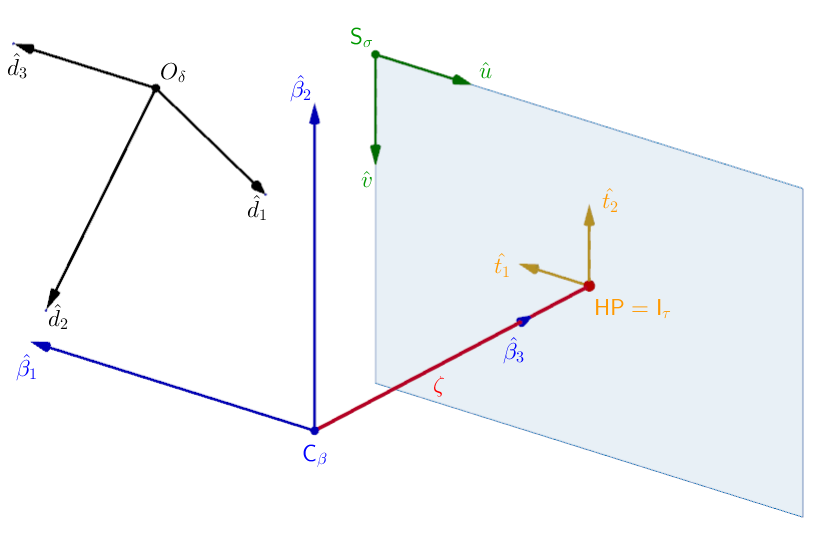
\includegraphics[width=0.8\linewidth]{images/UebersichtKoordinatensysteme_beschriftet.png}
	\captionof{figure}{Koordinatensysteme von einer Kamera aus im Überblick. Das Weltkoordinatensystem $(O,\delta)$ ist Deckungsgleich mit dem Kamerakoordinatensystem $(C,\beta)$}
	\label{fig:KoordinatensystemeUeberblick}
\end{minipage}\\ \\

%
%Grundlegend muss erst einmal festgelegt werden, welche Orientierungen die Koordinatensysteme haben sollen. Die Arbeit und auch die entstanden Algorithmen basieren auf rechtsdrehenden Systemen. Die Möglichkeit linksdrehende Systeme zu benutzen, ist aus dem entstandenen Algorithmus nicht ausgeschlossen, jedoch ist es für die spätere Deutung und Interpretation der Resultate wichtig im Vorhinein definiert zu haben, wie die Orientierung der einzelnen Koordinatensysteme ist. 
Das Weltkoordinatensystem $(O,\delta)$ ist mit $\delta = (\hat{d_1},\hat{d_2},\hat{d_3},O)$ definiert.
Die Kamerakoordinatensysteme der Kameras werden mit $(C,\beta)$ mit $(\beta = \hat{b_1},\hat{b_2},\hat{b_3},C)$ und $(C',\beta')$ mit $(\hat{b_1}',\hat{b_2}',\hat{b_3}',C')$ bezeichnet. Die Projektionszentren der Kameras entsprechen den Koordinatenursprüngen $C$ und $C'$, wie aus dem Lochkameramodell bekannt. Das zweidimensionale Bildebenenkoordinatensystem wird im weiteren Verlauf mit $(I,\tau)$ mit $\tau = (\hat{t_1},\hat{t_2},I)$ bezeichnet und zu guter Letzt fehlt noch das Sensorkoordinatensystem $(S,\sigma)$ mit $\sigma = (\hat{u},\hat{v},S)$.  Der Ursprung des Bildkoordinatensystem ist Deckungsgleich mit dem Hauptpunkt $HP$ auf der Bildebene. Der Ursprung des Sensorkoordinatensystems befindet sich in einer der Ecken der Bildebene. Das Bildebenenkoordinatensystem und das Sensorkoordinatensystem unterscheiden sich darin, dass das Sensorkoordinatensystem an die geometrie der Pixel auf dem Sensor angepasst ist und somit die Werte der Koordinatenachsen in Pixeleinheiten angegeben werden. Währendessen sind das Bildebenenkoordinatensystem, sowie auch die anderen hier vorgestellten Koordinatensysteme in dieser Arbeit immer in Millimeter definiert. Das Weltkoordinatensystem wird deckungsgleich mit dem Koordinatensystem von einer der beiden Kameras definiert, es gilt $(C,\beta)=(O,\delta)$.
 
%Jede der Bildebenen wird mit $<\hat{d_1},\hat{d_2}> + HP = I$ definiert, anhand dessen werden die Kamerakoordinatensysteme ausgerichtet. Die Achsen der Kamerkoordinatesysteme
%Des Weiteren soll gelten, dass \ensuremath{C_\beta = Z}, sprich der Ursprung des Kamerakoordinatensystems Deckungsgleich mit dem Projektionszentrum auf der Bildebene $I$ ist und somit auch \ensuremath{ <d_1,d_2> + P = I}. \ensuremath{P} bezeichent hier den Hauptpunkt der Bildebene. 

%Für die Wahl der Kamerakoordinatenachsen wird folgendes Schema verfolgt: \ensuremath{\hat{c}_1 \cdot \hat{n} = 0}, \ensuremath{\hat{c}_2 \cdot \hat{n} = 0}, \ensuremath{\hat{c}_3  = \pm\;\hat{n}}.  Die Bildebene selbst bekommt auch ein eigenes Koordinatensystem zugewiesen, welches sich aber nicht mehr auf einen 3D-Raum sondern auf die 2D-Ebene bezieht. Es soll \ensuremath{K_b = (\hat{b}_1,\hat{b}_2,O_b)} mit \ensuremath{O_b = P}, \ensuremath{\hat{b}_1 = \hat{c}_1}, \ensuremath{\hat{b}_2 = \hat{c}_2} gelten.  Formuliert man die Bildebene in Hess'scher Normalform so gilt \ensuremath{E: \hat{n} \cdot (\vec{x} - \vec{p}) = 0}. Als letztes kommt noch das Sensorkoordinatensystem mit  \ensuremath{K_s = (\vec{u}, \vec{v}, O_s)}. Dieses Koordinatensystem ist an die Geometrie der Pixel und des Sensors angepasst und daher muss es sich nicht unbedingt um ein kartesisches Koordinatensystem handeln. 

Nachdem die einzelnen Koordinatensysteme definiert sind, soll symbolisch die Projektion eines Objekts  aus dem 3D-Raum auf den 2D-Sensor aufgezeigt werden. Für die Transformation der Weltkoordinaten in Kamerakoordinaten gilt, dass $[\hat{d_1}\,\hat{d_2}\,\hat{d_3}\,1] \cdot R = [\hat{b_1}\,\hat{b_2}\, \hat{b_3}\, 1]$, wobei $R$ eine Tranformationsmatrix ist, wie sie im vorherigen Abschnitt eingeführt wurde. $R=[D|V]$, wobei $D$ eine $3 \times 3$-Rotationsmatrix darstellt und $V$ die Tranlationskomponente beschreibt. Der Translationsvektor \ensuremath{\vec{V}} besteht aus den Koordinaten des Projektionszentrums \textit{C}. Es gilt also $\vec{V} = C \leadsto \vec{v} = \begin{pmatrix}	C_{\delta,1}\\C_{\delta,2}\\C_{\delta,3}\end{pmatrix}$. 


(BEISPIEL BILDAUFNAHME IM ROTIERTEN SYSTEM)
 
\begin{gather} 		
%(d_1,d_2,d_3)[C] =(b_1, b_2, b_3) \leadsto b_1 = C_{11}d_1 + C_{21}d_2 + C_{31}d_3\\	
%\begin{bmatrix}
%\\C\\\\
%\end{bmatrix}
%=	\begin{bmatrix}
%\begin{pmatrix}
%\\
%c_1\\
%\\
%\end{pmatrix}_\delta
%\begin{pmatrix}
%\\
%c_2\\
%\\
%\end{pmatrix}_\delta
%\begin{pmatrix}
%\\
%c_3\\
%\\
%\end{pmatrix}_\delta
%\end{bmatrix}\\
(\hat{b_1}, \hat{b_2}, \hat{b_3},1)=(\hat{d_1},\hat{d_2},\hat{d_3},1) \cdot
\begin{bmatrix}
&  &  &C_{\delta,1} \\
&  [D]&  &C_{\delta,2} \\ 
&  &  &C_{\delta,3} \\
0&0&0 & 1
\end{bmatrix}	
\end{gather}

Ein Punkt $M_\delta$ Mit $M_\delta=[X_\delta,Y_\delta,Z_\delta,1]$ wird mit der soeben aufgestellten Transformationmatrix R=[D|V] zu einem Punkt $M_\beta$ transformiert.

\begin{gather}
M_\beta = M_\delta \cdot R\\
\begin{bmatrix}
X_\beta& Y_\beta& Z_\beta&1\\
\end{bmatrix} = 
\begin{bmatrix}
X_\delta& Y_\delta& Z_\delta&1\\
\end{bmatrix} \cdot
\begin{bmatrix}
	&  &  &C_{\delta,1} \\
	&  [D]&  &C_{\delta,2} \\ 
	&  &  &C_{\delta,3} \\
	0&0&0 & 1
\end{bmatrix}	
\end{gather}


Nach der Transformation eines Punkte $M_\delta$ in 3D-Kamerakoordinaten zu $M_\beta$, erfolgt nun die Porjektion des 3D-Kamerapunktes $M_\beta$ in die 2D-Bildebene zu $m_\tau$. Für die Projektion wird eine $3 \times 3$-Kameramatrix $K$ aufgestellt.  Es wird angenommen, dass $\zeta_x = \zeta_y =\zeta$
%Im nächsten Schritt müssen die Transformierten Kamerakoordinaten noch mit einer entsprechenden Kameramatrix $K$, welche die Punkte aus dem Kamerakoordinatensystem $(C,\beta)$ auf das Koordinatensystem der Bildebene $(I,\tau)$ mit $\tau = (t_1,t_2)$ projiziert, verrechnet werden. Hierzu muss eine entsprechende Kameramatrix $K$ aufgestellt werden. $\zeta$ erhält als Wert den Abstand des Projektionszentrums $Z$ zur Bildebene $I$.

	\begin{gather}
K = 
\leftidx{_{{I_\beta}}}{\begin{bmatrix}
	\pi
	\end{bmatrix}}{_{{C_\beta}}}
=
\begin{bmatrix}
\zeta&0&0&0\\
0&\zeta&0&0\\
0&0&\zeta&0\\
0&0&1&0
\end{bmatrix}\\
\begin{bmatrix}
\zeta&0&0&0\\
0&\zeta&0&0\\
0&0&\zeta&0\\
0&0&1&0
\end{bmatrix}
\begin{bmatrix}
X_\beta\\Y_\beta\\Z_\beta\\1
\end{bmatrix} =
\begin{pmatrix}
\zeta X\\ \zeta Y\\ \zeta Z \\ Z
\end{pmatrix}
=
\begin{bmatrix}
\zeta \frac{X}{Z}\\ \zeta \frac{Y}{Z}\\ \zeta  \\ 1
\end{bmatrix}
\end{gather}

Für die Koordinaten der Bildebene $I_\beta$ ergeben sich dann aus den Kamerakoordinaten $[\zeta \frac{X}{Z},\zeta\frac{Y}{Z},\zeta,1]^T$. Da die Koordinaten momentan noch in homogenen 3D-Koordinaten angegeben sind, aber das Bildebenenkoordinatensystem ein 2D-Koordinatensystem muss der Tiefenwert noch eliminiert werden. $\zeta$ gibt den Abstand von $C$ zu $I$ an, somit sind die 2D-Bildkorrdinaten des die Bildebenenkooridnatensystem  $[\zeta \frac{X}{Z},\zeta\frac{Y}{Z},1]^T = [X_\tau, Y_\tau,1]$. Zuletzt folgt in der Transformationskette noch die Transformation der Bildebenenkoordinaten in die Sensorkoordinaten mit dem Sensorkoordinatensystem $(S,\sigma)$ mit $\sigma = (\hat{u},\hat{v})$. $\hat{u}$ und $\hat{v}$ definieren die geometrische Beschaffung der Pixel, sie werdn auch als Vektoren $\vec{u}$ und $\vec{v}$ angegeben, somit muss das Sensorkoordinatensystem nicht zwangsläufig ein kartesisches Koordinatensystem sein. Die Werte $V_{\sigma,1}$ und $V_{\sigma,2}$ stehen für die Verschiebung des Koordinatensystemursprungs Hauptunkt auf der Bildebene in eine der Ecken der Bildebene.
		
		\begin{gather}
		\vec{u} = u_1 \hat{t_1} + u_2 \hat{t_2}\\
		\vec{v} = v_1 \hat{t_1} + v_2 \hat{t_2}\\
		S_\sigma = I_\tau +V_{\sigma,1} \hat{t_1} + V_{\sigma,2} \hat{t_2}\\
		\begin{pmatrix}
		\vec{u}, \vec{v}, 1
		\end{pmatrix}		
		=
		\begin{pmatrix}
		\hat{t_1}, \hat{t_2}, 1
		\end{pmatrix}\cdot	
		\begin{bmatrix}
		u_1&v_1&V_{\sigma,1}\\u_2&v_2&V_{\sigma,2}\\0&0&1\\
		\end{bmatrix}
		\end{gather}
		
		Der Koordinatenwechsel von Bildebenenkoordinaten in Sensorkoordinaten wird noch einmal Symbolisch veranschaulicht.	 
		
		Es wird ein Punkt $X_\sigma=\begin{pmatrix}
		a\\b\\1
		\end{pmatrix}$. In Sensorkoordinaten definiert. Die Transfomationsmatrix $M = \begin{bmatrix}
	u_1& v_1\\
	u_2& v_2
\end{bmatrix}$ beinhaltet statt einer Rotation eine Skalierung der Koordinatenwerte auf die Koordinaten des Sensorkoordinatensystems. Mit $M$ lässt sich wieder eine Projektionsmatrix $P$ aus einer Abbildungsmatrix $K$ mit einer Transformationsmatrix $M$ aufstellen. Ein Punkt $X_\tau$ wird in einen Punkt $X_\sigma$ transformiert.
	
		\begin{gather}
		X_\sigma =
		\begin{bmatrix}
		&  & \\
		&\begin{bmatrix}
		u_1& v_1\\
		u_2& v_2
		\end{bmatrix}^{-1}  & -M^{-1}\begin{pmatrix}
		V_{\sigma,1}\\V_{\sigma,2}
		\end{pmatrix} \\ 
		&  & \\
		0&0 & 1
		\end{bmatrix}
		\cdot
		X_\tau	
		\end{gather}\\
		
		 Die Projektionsmatrix $P$, welche die Kamerakoordinaten in Sensorkoordinaten überführt, wird dann wie folgt aufgebaut:\\
		
 	\begin{gather} 		
 		P 
		=
		\begin{bmatrix}
		&&\\
		&M^{-1}& -M\begin{pmatrix}V_{\sigma,1}\\V_{\sigma,2}\end{pmatrix}^{-1}\\
		&&\\
		0&0&1
		\end{bmatrix}
		\cdot
		\begin{bmatrix}
		-\zeta&0&0&0\\
		0&-\zeta&0&0\\
		0&0&1&0
		\end{bmatrix}
		=
		\begin{bmatrix}
		&&&0\\
		&-\zeta M^{-1}& -M\begin{pmatrix}V_{\sigma,1}\\V_{\sigma,2}\end{pmatrix}^{-1}&0\\
		&&&\\
		0&0&1&0
		\end{bmatrix}
		\end{gather}
	
%
%		
%		Zur Verdeutlichung folgen nun noch zwei Beispiele. Es werden $\vec{u}$ und $\vec{v}$, sowie $z_1$ und $z_2$ mit Werten versehen. $p$ entspricht symbolisch einem \textit{Pixelpitch}-Wert. Mit \textit{Pixelpitch} wird der direkte Abstand der Pixel auf Bildsensoren zwischen Pixelmitte zu Pixelmitte bezeichnet.\\
		
%		\underline{Beispiel 1:}\\
%		
%		$\vec{u} = 1pt_1 $\\
%		$\vec{v} = 2pt_2 $\\
%		$ p_1 = 15, p_2 = 20$\\
%		
%		Für die Projektionsmatrix $P$ ergibt sich somit:
%		
%		\begin{gather}
%		S_\sigma = I_\tau - \vec{u} - \vec{v} \leadsto S_\sigma = I_\tau -15 t_1 - 20 t_2\\	
%		M= 
%		\begin{bmatrix}
%		1&0\\
%		0&2
%		\end{bmatrix}
%		\leadsto
%		M^{-1}=\begin{bmatrix}
%		\frac{1}{p}&0\\
%		0&\frac{1}{2p}
%		\end{bmatrix}\\
%		K =
%		\leftidx{_{S_\sigma}}{\begin{bmatrix}
%				\pi
%		\end{bmatrix}}{_{I_\tau}} = 	
%		\begin{bmatrix}
%		\frac{-\zeta}{p}&0&15&0\\
%		0&\frac{-\zeta}{p}&20&0\\
%		0&0&1&0
%		\end{bmatrix}
%		\end{gather}\\
%		
%	 	\underline{Beispiel 2:}\\
%		
%		$\vec{v} = 1pt_1+2pt_2$\\
%		$\vec{u} = 1pt_1$\\
%		$ z_1 = 10, z_2 = 5$\\
%		
%		\begin{gather}
%		M=\begin{bmatrix}
%		1&1\\
%		0&2
%		\end{bmatrix} \leadsto 
%		M^{-1} =
%		\begin{bmatrix}
%		1&-\frac{1}{2}\\
%		0&\frac{1}{2}
%		\end{bmatrix} \\
%		K = \leftidx{_{S_\sigma}}{\begin{bmatrix}
%				\pi
%		\end{bmatrix}}{_{C_\beta}}
%		= 
%		\begin{bmatrix}
%		\frac{-\zeta}{p}&\frac{-\zeta}{2p}&10&0\\
%		0&\frac{-\zeta}{p}&5&0\\
%		0&0&1&0
%		\end{bmatrix}\\
%		= [K|0]
%		\end{gather}
		
		Die symbolische Darstellung der Projektionsmatrix von Welt in Sensorkoordinaten $	P = \leftidx{_{S_\sigma}}{\begin{bmatrix}
			\pi
			\end{bmatrix}}{_{O_\delta}}$ fügt sich somit aus dem vorhergehenden Abbildungsmatrix 
		K = $\leftidx{_{S_\sigma}}{\begin{bmatrix}
				\pi
		\end{bmatrix}}{_{C_\beta}}$ mit der Tranformationsmatrix $R$ zusammen.
		
		\begin{gather}
		\leftidx{_{S_\sigma}}{\begin{bmatrix}
			\pi
			\end{bmatrix}}{_{O_\delta}}
		=
		\leftidx{_{S_\sigma}}{\begin{bmatrix}
			\pi
			\end{bmatrix}}{_{C_\beta}}
		\cdot
		\begin{bmatrix}
		&&&\\
		&[C]^{-1}&& -[C]^{-1} Z\\
		&&&\\
		0&0&0&1\\
		\end{bmatrix}
		\end{gather}\\
		
	Somit ist die Transformations-Pipeline eines Punkte im Raum auf den Sensor einer Kamera am Ende. 
Zum Schluss hier noch einmal zum Vergleich die Darstellung der Projektionsmatrix $P$ aus \textit{Hartley\&Zisserman}\cite{HZ}. Zu beachten ist hier, dass im \textit{Hartley\&Zisserman} $R$ für $[R]^{-1}$ steht\cite{HZ}.
		
		\begin{gather}
		\begin{split}	
		P=
		[K|0] \begin{bmatrix}
		&&&\\
		&R&&-RZ\\
		&&&\\
		0&0&0&1\\
		\end{bmatrix}\\
		=[KR|-KRZ] 	= KR[I_{3x3}|-Z]
		\end{split}
		\end{gather}

		
		% C1 - example 2
		\chapter{Herstellen geometrischer Beziehungen zwischen Punktekorrespondenzen zweier Aufnahmen}

Das Ziel dieser Masterarbeit ist es Punkte im dreidimensionalen Raum aus einer Stereoskopischen Aufnahme zweier Kameras zu rekonstruieren.Bis jetzt wurde nur die Bildaufnahme einer Kamera betrachtet. Jedoch kann eine Kamera allein nicht räumlich sehen. Um Räumlichkeit aus Bilder zu rekonstruieren, müssen mindestens zwei Aufnahmen der gleichen Szene aus unterschiedlichen Blickwinkeln aufgenommen werden. Des Weiteren wir davon ausgegangen, dass

 . Um eine Beziehung zwischen zwei Aufnahmen herzustellen, werden Korrespondezen benötigt.  Das bedeutet es wird versucht einen Punkt in der einen Aufnahme in einen Punkt in der anderen zu überführen. Die extrinsischen und intrinsischen Kameraparameter müssen hierfür nicht unbeding bekannt sein. Es werden hierzu verschiedenen Falle betrachtet. Zum einen ...

\section{Homographien}
\label{sec:homographien} 

Im vorherigen Kapitel wurde mathematisch die Projektion eines 3D-Punktes in einen 2D-Bildpunkt auf einem Kamerasensor durch Koordinatentransformation aufgezeigt. Im nächsten Schritt soll die Beziehung zwischen dem projizierten 3D-Punkt in zwei perspektivische Kameras und den entstehenden 2D-Bildpunkten genauer erläutert werden. Die 2D-Bilder des projizierten 3D-Punktes sind abhängig vom Aufbau der abgebildeten Szene und den Positionen und Ausrichtungen der Kameras\cite{Elements}. Die Beziehung zwischen einem 3D-Punkt und seinen projektionen auf zwei Kameras, kann in einer sogenannten Homographie beschrieben werden. Die Homographie gilt jedoch nur für die Projektion einer planaren Szene im 3D-Raum auf auf zwei Kamerasensoren. Als Homographie wird eine projektive Transformation zwischen zwei Ebenen bezeichnet. Dabei bleiben Kollinearitäten und die Reihenfolge von Punkten auf Geraden, wie zum Beispiel Schnittpunkte mit anderen Geraden, erhalten. Bei den Ebenen handelt sich in diesem Fall um die Bildebenen des Kameramodells. Aufgrund dieser Ebenenannahme, kann solch eine projektive Transformation durch eine 3x3-Homograohiematrix ausgedrückt werden\cite{Roser}. Die Homograohiematrix $H$, projiziert jede Figur in eine Figur gleicher projektiver Entsprechung\cite{HZ,Elements}. Sind die Punkte $A',B',C'$ und $D'$ die projektiven Bilder eines Systems von vier kollinearen Punkten, so ist $(A',B',C',D') = (A,B,C,D)$\cite{Peiffer}. Der Grund warum Homographien in dieser Arbeti eingeführt werden ist, dass sie elementar sind wenn es darum geht Transformationen auf den Bildebenen der Kamera durchzuführen, wie es im Kapitel \nameref{sec:rectification} für die geometrische Entzerrung zweier Bilder von Nöten ist.Außerde bildet ihre geometrische Herleitung eine gute Brücke zur \nameref{sec:epipolar}, welche im nachfolgenden Kapitel vorgestellt wird und der Elementare Baustein für die Stereobildanalyse bildet. Mit Hilfe der Homography ist es möglich eine Beziehung zwischen den zwei projizierten 2D-Bildpunkten herzuleiten, ohne das intrinsische Parameter in Form einer Kamermatrix $K$ noch die extrisischen Parameter in Form der Matrix $R$ bekannt sind\cite{HZ,Elements}.  Diese können dann wiederum aus der, durch die Bildpunkte beider Kameras, entstandenen Homographiematrix geschätzt werden\cite{HZ}. Die Homographie fasst die Transformationen wie Rotation und Translation, sowie die jeweiligen Abbildungsmatrizen der Kameras in einer 3x3-Matrix zusammen.\cite{Elements,Peiffer}. 


Es seien \ensuremath{m_{\tau} = \begin{pmatrix}
		m_{\tau,1}\\m_{\tau,2}\\m_{\tau,3}
\end{pmatrix}} die homogenen Koordinaten eines Punktes auf der Bildebene$(I,\tau)$ und \ensuremath{m'_{\tau'} = \begin{pmatrix}
m'_{\tau',1}\\m'_{\tau',2}\\m'_{\tau',3}
\end{pmatrix}} ein Punkt der projektiv transformierten Bildebene $(I',\tau')$. Dann gilt

\begin{gather}
	m'_{\tau'} = Hm_{\tau}\\
	Hm_{\tau} = \begin{bmatrix}
	{h_1}^T \cdot m_{\tau}\\{h_2}^T \cdot m_{\tau}\\{h_3}^T \cdot m_{\tau}
	\end{bmatrix} \\
	\leadsto 
	m'_{\tau'}= Hm_{\tau}= \begin{bmatrix}
	h_{11}m_{\tau,1}+h_{12}m_{\tau,2}+h_{13}m_{\tau,3}\\
	h_{21}m_{\tau,1}+h_{22}m_{\tau,2}+h_{23}m_{\tau,3}\\
	h_{31}m_{\tau,1}+h_{32}m_{\tau,2}+h_{33}m_{\tau,3}
	\end{bmatrix}\\
	\leadsto 
	H=\begin{bmatrix}
	h_{11}&h_{12}&h_{13}\\
	h_{21}&h_{22}&h_{23}\\
	h_{31}&h_{32}&h_{33}
	\end{bmatrix}
\end{gather}

Dabei müssen die Koeffizienten so geartet sein, dass die zugehörige Transformation umkehrbar ist\cite{HZ}\cite{Peiffer}.
\begin{gather}
	m'_{\tau'}=Hm_\tau\\
	m_\tau= H^{-1}m'_{\tau}
\end{gather}\\


(GRAFIK NOCH ANPASSEN MIT $m_\beta$ etc)\\


\begin{figure}[!htb]
	\minipage{0.48\textwidth}
	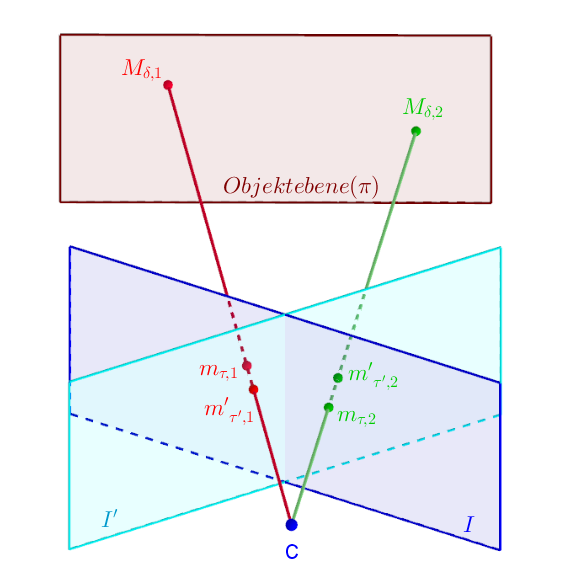
\includegraphics[width=\linewidth]{images/HomographyPZ_beschriftet.png}
	%	\caption{A really Awesome Image}
	\label{fig:HomographyPZFront}
	\endminipage\hfill
	\minipage{0.54\textwidth}
	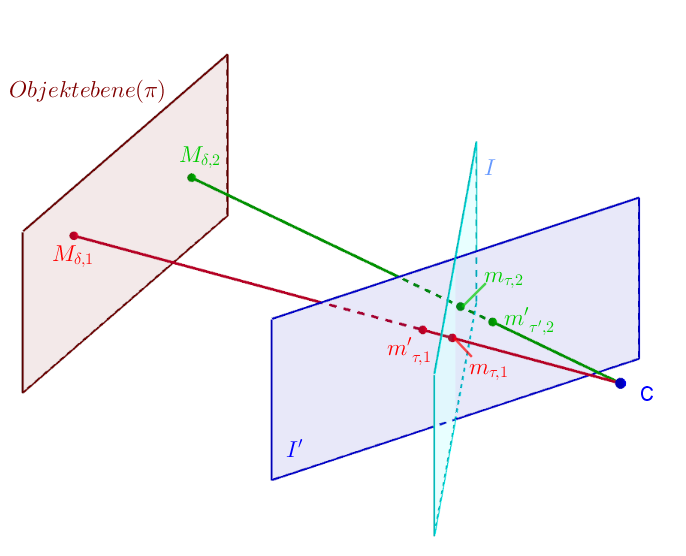
\includegraphics[width=\linewidth]{images/HomographyPZSide_beschriftet.png}
	%	\caption{A really Awesome Image}
	\label{fig:HomographyPZSide}
	\endminipage\hfill
	\caption{Die Abblildung zeigt zwei Aufnahmen einer um ihr Projektionszentrum $C$ gedrehten Kamera. Die zwei blauen Ebenen stellen jeweils die Bildebene vor und nach der Drehung dar sie wird einmal als Bildebene $(I,\tau)$ und einmal als Bildebene $(I',\tau')$ bezeichnet. Die Objektebene befindet sich im 3D-Raum, dementsprechend sind die Punkte $M_{1,\delta}$ und $M_{2,\delta}$ in homogenen 3D-Koordinaten gegeben. Die Punkte $m_{1,\tau}$ und $m_{2,\tau}$ sind die projizierten Puntke auf der Bildebene $(I,\tau)$ und Die Punkte $m_{1,\tau'}$ und $m_{2,\tau'}$ sind die projizierten Punkte auf der Bildebene $(I',\tau')$}
	\label{fig:homographyRotatedProjectionCenter}
\end{figure}

Um die Herleitung der Homographiematrix zu veranschaulichen, werden zwei unterschiedliche Fälle betrachtet. Der erste Fall ist in Abbildung \ref{fig:homographyRotatedProjectionCenter} gezeigt. Eine planare Szene im Raum soll auf die Bildebene $(I,\tau)$ einer Kamer projiziert werden, danach wird die Kamera um ihr Projektionszentrum gedreht die 3D-Objektpunkte somit auf die neu ausgerichtet Bildebene $(I,\tau')$ projiziert. Im zweiten Fall wird die Kamera nicht um ihr Projetionszentrum gedreht, sondern um einen definierten Drehpunkt, so dass zu der Rotation noch eine zusätzliche Translation der Kamera erfolgt. Für Fall eins wird zunächst angenommen, dass die Transformationsmatrizen $R$ und $R'$ sowie die Kameramatrizen $K$ und $K'$ bekannt sind. $m_\tau$ und $m'_{\tau'}$ sind die projizierten Punkte von $M_\delta$ auf den Bildebenen $(I,_tau)$ mit $\tau=(\hat{t_1},\hat{t_2},I)$ und $(I',_\tau')$ mit $\tau=(\hat{t_1}',\hat{t_2}',I)$. Die Kamerakoordiantensyteme werden definiert als $(C,\beta)$ mit $\beta = (\hat{b_1},\hat{b_2},\hat{b_3},C)$, wobei $\hat{b_3} = \overline{CI}$ ist und $(C',\beta')$ mit $\beta' = (\hat{b_1}',\hat{b_2}',\hat{b_3}',C')$, wobei $\hat{b_3}' = \overline{C'I'}$\cite{Elements}. 

% jedoch werden für die Rechnung eine andere Darstellung von $m$ und $m'$ verwendet. Die zu dem zweidimensionalen Bildebenkoordinatensystemen $(I,\tau)$ und $(I',\tau')$ korrespondierenden dreidimensionalen Kamerakoordinatensysteme $(C,\beta)$ mit $\beta = (\hat{b_1},\hat{b_2},\hat{b_3},\overline{IC})$ und $(C',\beta')$ mit $\beta' = (\hat{b_1}',\hat{b_2}',\hat{b_3}',\overline{I'C'})$ werden für die Herleitung verwendet.
% 
%  Diese Koordinatensysteme stellt die Bildebenenpunkte $m_\beta$ und $m'_{\beta'}$ wie im Kapitel \nameref{sec:basisTransformation} Gleichung 3.26 dar. Da in dieser Darstellung $\hat{b_1} = \hat{t_1} $ und $\hat{b_2} = \hat{t_2}$ ist, kommt es zu keinen Komplikationen. Die Koordinaten bleiben die selben nur werden sie aus dem 3D-Koordinatensystem der Kameras beschrieben und bekommen somit die Tiefenkomponeten $\zeta$ und $\zeta'$ wieder dazu. Der Grund warum diese Koordinatendarstellung für die Bildpunkte gewählt wird, ist das so vermieden wird, dass es zu konflikten der Dimensionen der Matrizen $R$ und $R'$ sowie $K$ und $K'$ und den Punkten $m_\beta$ und $m'_\beta$ kommt\cite{Elements}. 
  
Die folgenden Gleichungen 4.7 und 4.8 zeigen wieder die bereits bekannte Projektion eines 3D-Punktes auf die 2D-Bildebene, jedoch werden die projizierten Punkte $m_\beta$ und $m_{\beta'}$ noch bezüglich der dreidimensionalen Kamerakoordinatensysteme dargestellt. $\zeta$ und $\zeta'$ repräsentieren jeweils die Tiefe von $m_\beta$ und $m'_{\beta'}$, welche gegen Ende eliminiert wird\cite{Elements}.


\begin{gather}
\zeta \vec{m}_\beta = P \begin{bmatrix}\vec{M}_\delta\\1\end{bmatrix} = 
\begin{bmatrix}KR|-KR\vec{C}_\delta\end{bmatrix}\cdot \begin{bmatrix}\vec{M}\delta\\1\end{bmatrix} = KR(\vec{M}\delta - \vec{C}_\delta)\\
\zeta' \vec{m'_{\beta'}} = P' \begin{bmatrix}\vec{M'}_\delta\\1\end{bmatrix} = 
\begin{bmatrix}K'R'|-K'R'\vec{C}_\delta\end{bmatrix}\cdot \begin{bmatrix}\vec{M}\delta\\1\end{bmatrix} = K'R'(\vec{M}\delta - \vec{C}_\delta)
\end{gather}


Der Vektor $(\vec{M}\delta - \vec{C}_\delta)$, beschreibt die Verbindung zwischen dem Objektpunkt $M_\delta$  und dem Projektionszentrum $C_\delta$. Die Gleichungen 4.7 und 4.8 können auf Grund ihrer identischen Projektionszentren jeweils nach  $(\vec{M}\delta - \vec{C}_\delta)$ aufgelöst werden 

\begin{gather}
	\zeta RK^{-1}\vec{m_\beta} = \vec{M}_\delta - \vec{C}_\delta\\
	\zeta' R'K'^{-1}\vec{m'_{\beta'}} = \vec{M}_\delta - \vec{C}_\delta
\end{gather}

Da die Rechten seiten der Gleichungen 4.9 und 4.10 identisch sind, können die linken Seiten gleichgesetzt werden.

\begin{gather}
	\zeta' R'K'^{-1}\vec{m'_{\beta'}}=\zeta RK^{-1}\vec{m_\beta}\\
\end{gather}

Um nun die gewünschte Form von $m'_{\tau'} = Hm_{\tau}$ zu bekommen, wird die Gleichung nach $	\frac{\zeta'}{\zeta}\vec{m'_{\beta'}}$ aufgelöst.

\begin{gather}
	\frac{\zeta'}{\zeta}\vec{m'_{\beta'}} = K'R'R^TK^{-1}\vec{m}_\beta\\
\lambda \vec{m'}_{\beta'} = H\vec{m}_\beta\\
\leadsto m'_{\tau'} = H m_\tau
\end{gather}

Es Resultiert also dass wenn $\lambda = \frac{\zeta'}{\zeta}$, dann gilt dass $H = K'R'R^TK^{-1}$ gleicht. Gilt nun noch der Fall, dass $K = K'$ ist, dann reduziert sich $H$ zu $K^{-1}HK = R'R$, welches einer Rotation gleicht.\cite{Elements}. 




\section{Abbildungsunterschiede bei verschobenen Rotationsachsen}

Wie am Anfang des Kapitels erwähnt, sollen zwei verschiedene Fälle für die Homographie betrachtet werden. Der Grund sind, die unterschiedlichen Abbildungsmerkmale die bei einer Drehung um das Projektionszentrum und einer Drehung um einen definierten Drehpunkt entstehen. Die Frage ist, ob und wie sich beim zweiten Fall eine Homographiematrix herleiten lässt und in wie fern sie sich von der bereits bekannten Herleitung unterscheidet. Um zu veranschaulichen, was genau sich bei einer Drehung um ein Drehpunkt und der Drehung um das Projektionszentrum ändert, wurde eine Simulation geschrieben, welche die Abbildungsunterschiede beider Drehungen aufzeigt. Abbildung \ref{fig:SimulationAnfang} zeigt die Ausgangssituation der Simulation. In einen virtuellen Raum wurde eine Kamera platziert, welche auf ein Objekt gerichtet ist. Dieses Objekt besteht aus deinem Quadrat, das durch die schwarzen Eckpunkte begrenzt ist. In der Mitte des Quadrats wurde mit Rot der Mittelpunkt des Quadrats gekennzeichnet. Dieser Mittelpunkt symbolisiert den Drehpunkt um welchem sich die Kamera später drehen soll. 

\begin{minipage}{\linewidth}
	\centering
	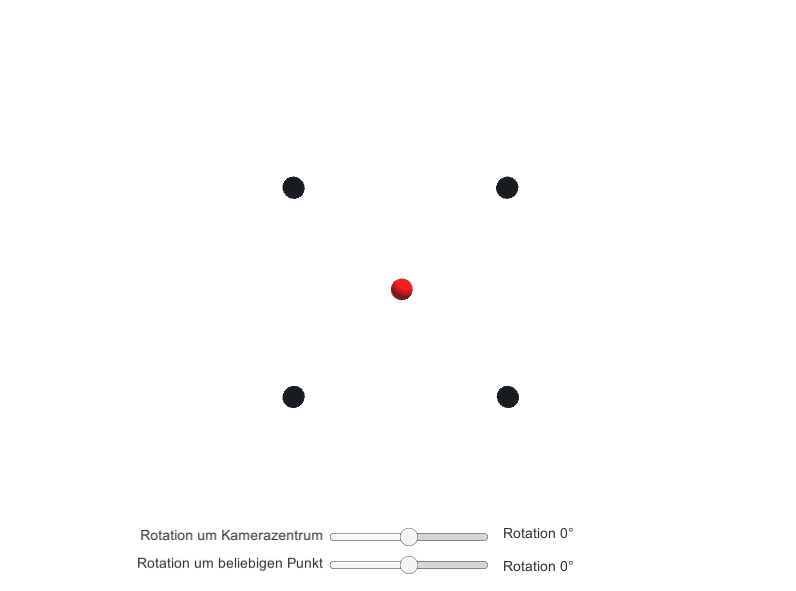
\includegraphics[width=.8\linewidth]{images/Ausgangslage.png}
	\captionof{figure}{Ausgangsituation der Simulation}
	\label{fig:SimulationAnfang}
\end{minipage}\\

%Im folgenden soll zunächst die Abbildungsunterschiede der entstehenden 2D-Bilder, bei den zwei genannten unterschiedlichen Fällen aufgezeigt werden.
%
%
%Bis jetzt wurden die Kameras jeweils nur um ihr Projektionszentrum gedreht, die Frage die jetzt noch im folgenden beantwortet werden soll ist, ob es ebenfalls möglich ist eine Homographiematrix für korrespondierende Punktepaare in einer Ebene aufzustellen, wenn eine Kamera um einen spezifischen Drehpunkt außerhalb der Kamera gedreht wurde. 
%
%In diesem Fall wären die beiden Projektionszentren $(C,\beta)$ und $(C',\beta')$ der Kameras nicht mehr identisch.  Des Weiteren soll geklärt werden, ob Punkte die bei der Drehung um das Projektionszentrum verdeckt bleiben auch bei einer Drehung um einen außerhalb der Kamera platzierten Drehpunkt verdeckt bleiben. In der Simulation ist der rote Punkte in der Mitte des Quadrats der Drehpunkt, wie in Abbildung \ref{fig:SimulationAnfang} dargestellt ist. 

Für die Simulation der unterschiedlichen Drehungen wurden zwei Schieberegler implementiert mit denen sich die Kamera einmal um ihr Projektionszentrum, und einmal um den Drehpunkt drehen lässt. Abbildung \ref{fig:DrehungProjektionszentrum} zeigt jeweils die entstehenden Bilder, wenn die Kamera um \ensuremath{20^\circ} beziehungsweise \ensuremath{-20^\circ} um das Projektionszentrum gedreht wurde.


\begin{minipage}{\linewidth}
	\centering
	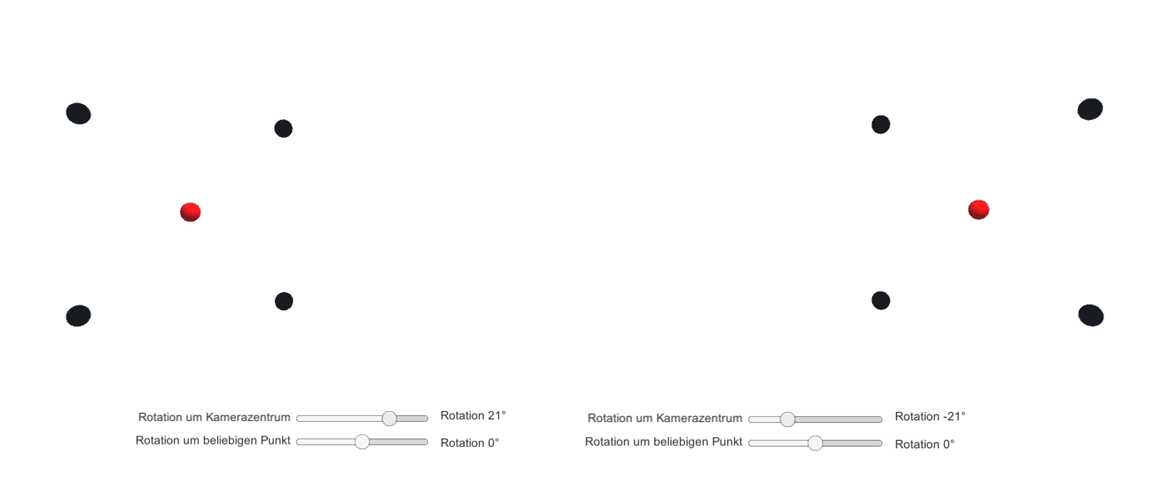
\includegraphics[width=1.\linewidth]{images/DrehungPZ.png}
	\captionof{figure}{Drehung um das Projektionszentrum}
	\label{fig:DrehungProjektionszentrum}
\end{minipage}\\ \\

Abbildung \ref{fig:DrehungDrehpunkt} zeigt die entstehenden Bilder, wenn die Kamera um \ensuremath{45^\circ} beziehungsweise \ensuremath{-45^\circ} um den Drehpunkt gedreht wurde. Wie sich zeigt ist hier ein weiterer grüner Punkt zu sehen welcher zu Testzwecken hinter dem roten Punkt platziert wurde sichtbar.

\begin{minipage}{\linewidth}
	\centering
	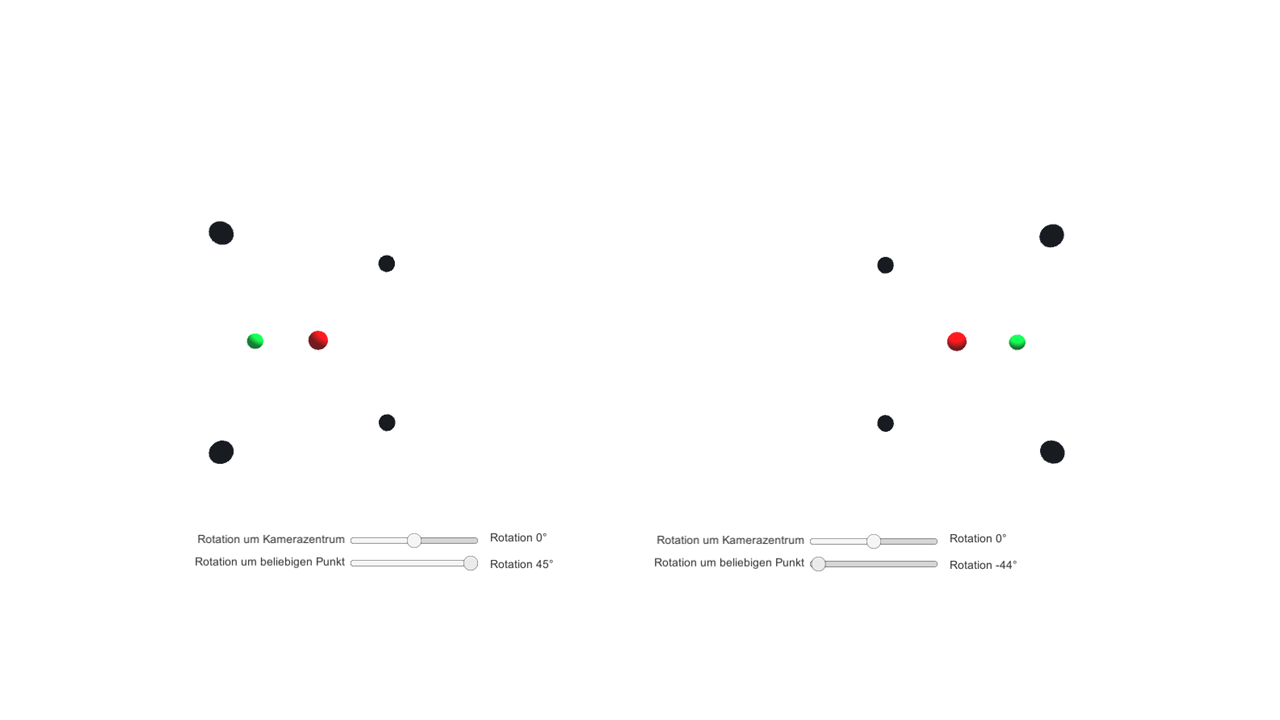
\includegraphics[width=1.\linewidth]{images/DrehungDZ.png}
	\captionof{figure}{Drehung um einen Drehpunkt. In diesem Beispiel wurde der rote Punkt als Drehpunkt verwendet}
	\label{fig:DrehungDrehpunkt}
\end{minipage}\\ 

Punkte die bei einer Drehung um das Projektionszentrum verdeckt bleiben, können bei einer Drehung um einen außerhalb der Kamera liegenden Drehpunkt sichtbar werden. Die Abbildungen \ref{fig:Strahlengang1} und \ref{fig:Strahlengang2} veranschaulichen anhand von Strahlenoptik, was der Grund für die Verdeckung ist. \\


\begin{figure}[!htb]
	\minipage{0.48\textwidth}
	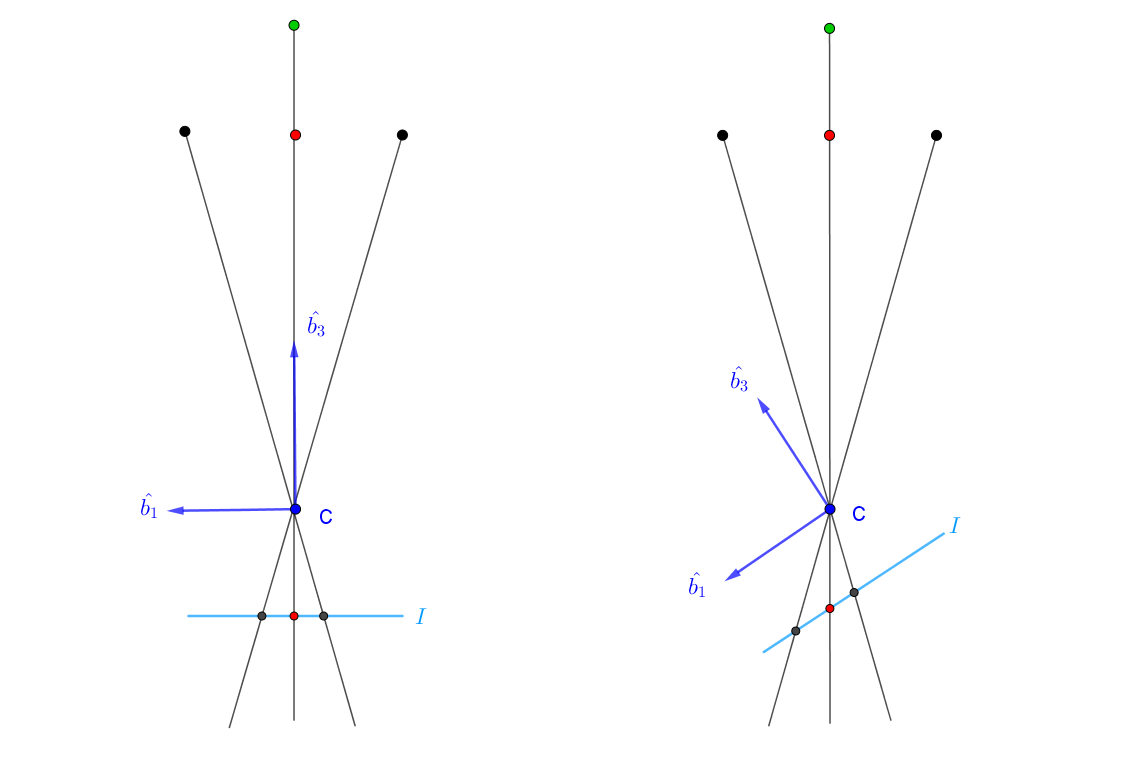
\includegraphics[width=\linewidth]{images/GrafikDrehungProjektionszentrum.png}
	\captionof{figure}{Strahlengang durch das Projektionszentrum. Auf der Abbildung ist erkennbar, dass der grüne Punkt auch nach der Drehung der Kamera um das Projektionszentrum vom roten Pukt verdeckt bleibt}
	\label{fig:Strahlengang1}
	\endminipage\hfill
	\minipage{0.5\textwidth}
	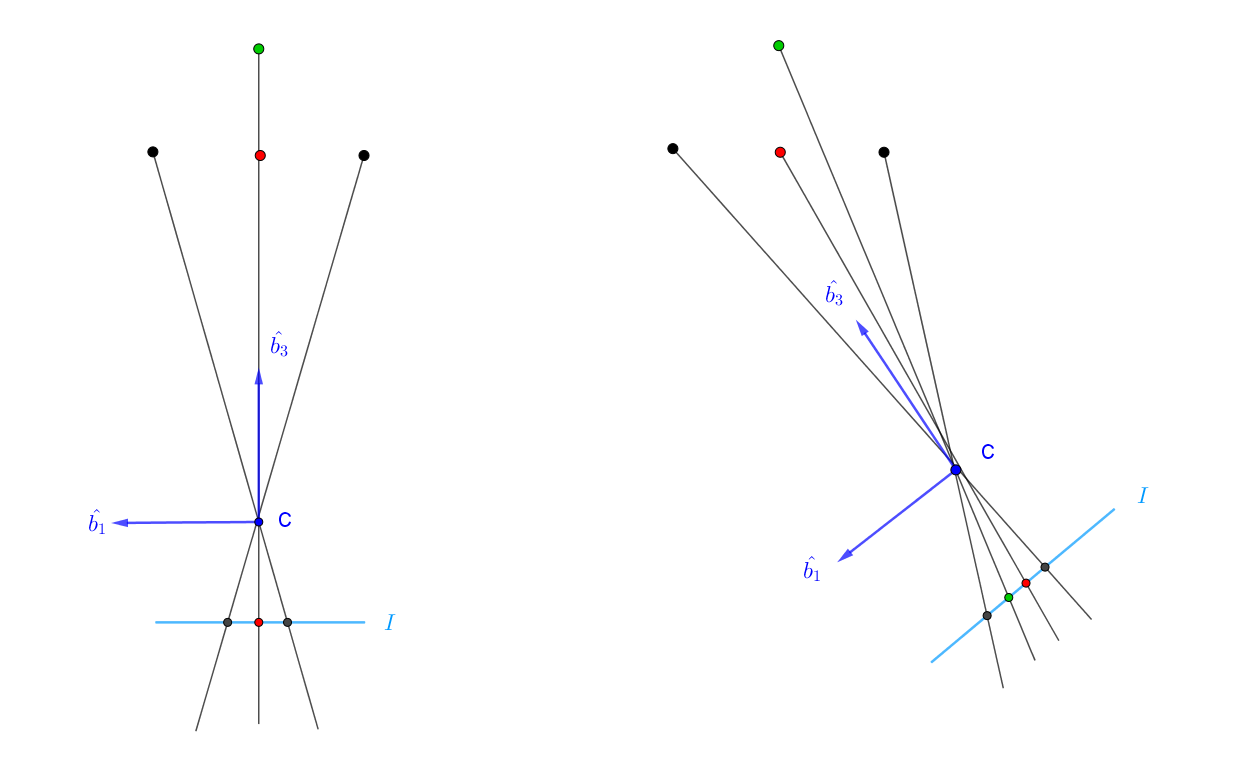
\includegraphics[width=\linewidth]{images/GrafikDrehungUmDrehpunkt.png}
		\captionof{figure}{Strahlengang durch das Projektionszentrum. Auf der Grafik ist erkennbar, dass der grüne Punkt nach der Drehung der Kamera um einen Drehpunkt, welcher in diesem Fall der rote Punkt darstellt, sichtbar wird.}
	\label{fig:Strahlengang2}
	\endminipage\hfill
\end{figure}

Die Bildebene ist in diesem Beispiel hinter dem Projektionszentrum platziert. Die Lage der Bildebene ist in sofern egal, dass es sei sie im gleichen Abstand vor oder hinter dem Projektionszentrum, immer zur selben Abbildung kommt. Jedoch ist die Abbildung, bei hinter dem Projektionszentrum platzierten Bildebene, auf dem Kopf abgebildet. Die Positionierung hinter das Projektionszentrum dient allein der Übersichtlichkeit der Abbildungen, im restlichen Verlauf der Arbeit wird die Bildebene immer vor das Projektionszentrum platziert um Verwirrungen zu vermeiden. Der grüne Punkt wurde nur als Beweis platziert, dass sich die entstehenden Abbildungen beider Fälle voneinander unterscheiden. Für den weiteren Verlauf wird er nicht weiter beachtet. Für die Homographie gelten nur die Punkte, welche sich im Raum auf einer Ebene befinden. Im folgenden wird eine Herleitung der Homographiematrix für den zweiten Fall aufgestellt. 

\begin{minipage}{\linewidth}
	\centering
	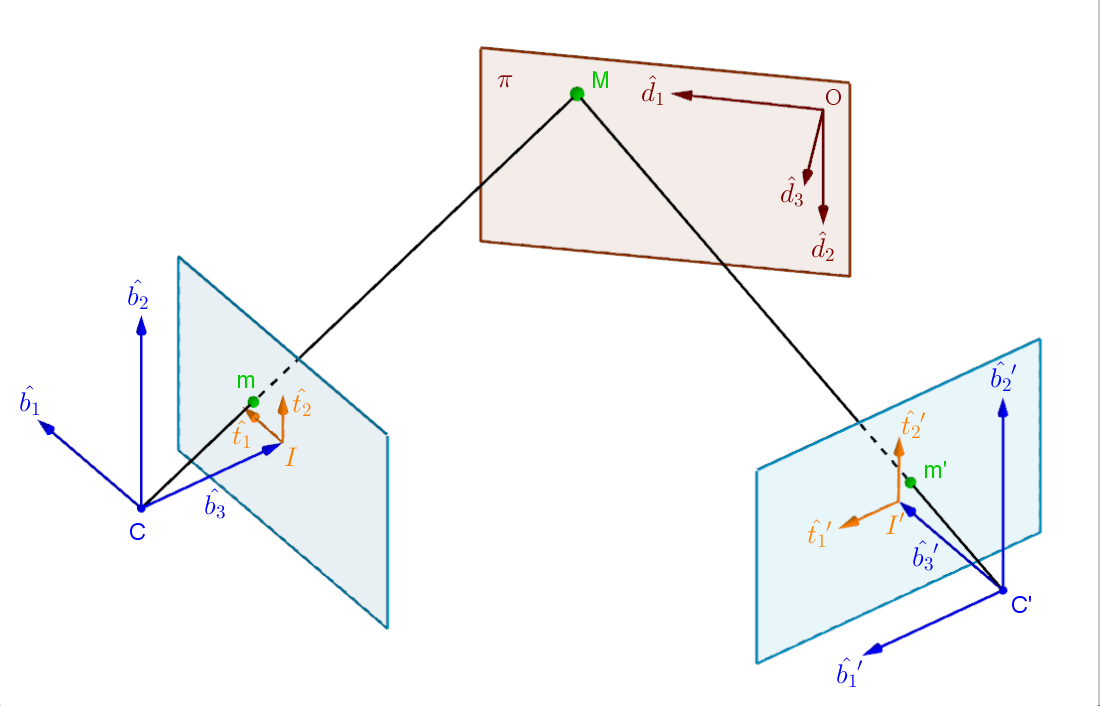
\includegraphics[width=0.8\linewidth]{images/HomographieDP_beschriftet.png}
	\captionof{figure}{Veranschaulichung der Homographie bei zwei verschieden translatierten und rotierten Kameras.}  
\end{minipage}\\

Angenommen es existiert eine Ebene $\pi$ im Raum mit einem Objektpunkt $M_\delta$ bezüglich eines Weltkoordinatensystems $(O,\delta)$ mit $\delta = (\hat{d_1},\hat{d_2},\hat{d_3},O)$. $\hat{d_1}$ und $\hat{d_2}$ spannen Die Ebene $\pi$ auf. Der Punkt $M_\delta$ wird nun mit den Projektionsmatrizen $P = [KR|-KR\vec{C}_\delta]$ und $P'=	[K'R'|-K'R'\vec{C}_\delta]$ in einen Punkt bezüglich der Bildebenen $(I,\tau)$ mit $\tau = (\hat{t_1}, \hat{t_2},I)$ und $(I',\tau')$ mit $\tau' = (\hat{t_1}', \hat{t_2}',I')$ projiziert. auch hier gilt wie im vorherigen Beispiel, dass die projizierten Bildkoordinaten als $m_\beta$ und $m'_{\beta'}$ der jeweiligen Kamerakoordinatensysteme $(C,\beta)$ mit $\beta = (\hat{b_1},\hat{b_2},\hat{b_3},C)$, wobei $\hat{b_3} = \overline{CI}$ und $(C',\beta')$ mit $\beta' = (\hat{b_1}',\hat{b_2}',\hat{b_3}',\overline{C'I'})$, wobei $\hat{b_3}' = \overline{C'O}$, dargestellt werden. Da der Ursprung des Weltkoordinatensystem $(O,\delta)$ auf der Ebene $\pi$ liegt und $\hat{d_1}$ und $\hat{d_2}$ diese aufspannen, gilt für den Punt $M_\delta$ auf $\pi$ $M_\delta = \begin{pmatrix}
x_{\hat{d_1}}\\
y_{\hat{d_2}}\\
0
\end{pmatrix}$. die Bezeichnungen $p_i$ und $p_i'$ stehen im folgenden für die einzelnen Spalten der Projektionsmatrizen $P$ und $P'$. Für die Projektion des Punktes $M_\delta$ in die Bildpunkte  $m_\beta$ und $m'_{\beta}$ bezüglich $(C,\beta)$ und $(C',\beta')$ gelten die folgenden beiden Gleichungen\cite{Elements}.


\begin{gather}
\zeta m_\beta = P \cdot 
\begin{bmatrix}
	M_\delta\\1
\end{bmatrix} = 
\begin{bmatrix}
	p_1&p_2&p_3&p_4
\end{bmatrix} \cdot
\begin{bmatrix}
	x_\delta\\y_\delta\\0\\1
\end{bmatrix}=
\begin{bmatrix}
	p_1&p_2&p_4
\end{bmatrix} \cdot
\begin{bmatrix}
	x_\delta\\y_\delta\\1
\end{bmatrix}=
G \vec{m}_\tau\\
\zeta' m'_{\beta'} = P \cdot 
\begin{bmatrix}
	M_\delta\\1
\end{bmatrix} = 
\begin{bmatrix}
	p'_1&p'_2&p'_3&p'_4
\end{bmatrix} \cdot
\begin{bmatrix}
	x_\delta\\y_\delta\\0\\1
\end{bmatrix}=
\begin{bmatrix}
	p'_1&p'_2&p'_4
\end{bmatrix} \cdot
\begin{bmatrix}
	x'_\delta\\y'_\delta\\1
\end{bmatrix}=
G' \vec{m}'_{\alpha}\\
\end{gather}\\

In diesem Prozess sind sowohl die zwei Matrizen $G$ und $G'$, sowie zwei weitere Koordinatensysteme $(C,\alpha)$ mit $\alpha = (\hat{d_1},\hat{d_2},\hat{d_4})$, wobei $\hat{d_4} = \overline{CO}$ und  $(C',\alpha')$ mit $\alpha' = (\hat{d_1},\hat{d_2},\hat{d_4}')$, wobei $\hat{d_4}' = \overline{C'O}$ entstanden\cite{Elements}.
Des Weiteren sind zwei neue Punkte $m_\alpha$ und $m'_{\alpha}$ entstanden, von denen behauptet wird, dass $\zeta m_\beta = G\cdot m_\alpha$ und $\zeta' m'_{\beta'} = G'\cdot m'_{\alpha'}$ gelte\cite{Elements}. Um dies zu testen werden $m_\alpha$ und $m'_{\alpha}$ anders formuliert.

\begin{gather}
	m_\alpha = M_\alpha + \overline{CO}_\alpha = M_{(\hat{d_1},\hat{d_2},\hat{d_4})} + \overline{CO}_{(\hat{d_1},\hat{d_2},\hat{d_4})} = \begin{pmatrix}
		x_\delta\\
		y_\delta\\
		1
	\end{pmatrix} \\
	m'_{\alpha'} = M_{\alpha'} + \overline{CO}_{\alpha'} = M_{(\hat{d_1},\hat{d_2},\hat{d_4}')} + \overline{CO}_{(\hat{d_1},\hat{d_2},\hat{d_4}')} = \begin{pmatrix}
	x_\delta\\
	y_\delta\\
	1
\end{pmatrix} 
\end{gather}

Aus Gleichungen 4.18 und 4.19 folgt dann, dass für alle Punkte in der Ebene $\pi$ gilt, dass $m_\alpha = m'_{\alpha}$. Woraus für die Punkte $\zeta m_\beta$ und $\zeta' m'_{\beta'}$ folgt, dass $\zeta m_\beta = G\cdot m_\alpha$ und $\zeta' m'_{\beta'} = G'\cdot m'_{\alpha'}$\cite{Elements}. Somit kann für $\zeta m_\beta$ und $\zeta' m'_{\beta'}$ folgende Beziehungsgleichung aufgestellt werden\cite{Elements}.

\begin{gather}
	\zeta' m'_{\beta'} = G' G^{-1} \zeta m_\beta
\end{gather}

Für $\frac{\zeta'}{\zeta} = \lambda$, kann Gleichung 4.20 dann wieder umformuliert werden in:

\begin{gather}
	\lambda m'_{\beta'} = H m_\beta\\
	\leadsto m'_{\tau'} = H m_\tau
\end{gather} 

Zwei projizierte Bilder einer Ebene sind also über eine Homographie $H$ miteinander verwandt, welche wiederum eine Kombination aus denjenigen Homographien ist, welche die jeweiligen Bilder mit der Ebene $\pi$ in Beziehung setzten\cite{Elements}.
 
\section{Berechnung der Homographiematrix aus Bildebenenkoordinaten}

Hier sagen wo man die Punkte herbekommt

Nachdem nun bekannt ist, wie eine Homographie Beziehungen zwischen projizierten Punkte beschreiben kann, wird im nächsten Schritt davon ausgegangen, dass die Transformationsmatrizen $R$ und $R'$ sowie die Kameramatrizen $K$ und $K'$ nicht bekannt sind. Es wird schematisch aufgezeigt, wie die Homographiematrix aus 2D-Bildpunkte gewonnen werden kann. Um eine Homographiematrix mit 
$H=
\begin{bmatrix}
h_{11}&h_{12}&h_{13}\\
h_{21}&h_{22}&h_{23}\\
h_{31}&h_{32}&h_{33}
\end{bmatrix}
$ zu erhalten werden die Punkte beider Kameras in eine Koeffizientenmatrix $A$ eingetragen, welche sich nach dem in den Gleichungen 4.25 bis 4.34 laufenden Schema aufstellen lässt. 

\begin{gather}
	H\cdot m_\tau = m'_{\tau}\\
	\begin{bmatrix}
		h_{11}&h_{12}&h_{13}\\
		h_{21}&h_{22}&h_{23}\\
		h_{31}&h_{32}&h_{33}
	\end{bmatrix}
	\cdot
	\begin{bmatrix}
		\\m_\tau\\\\
	\end{bmatrix}
	=
	\begin{bmatrix}
		\\m'_{\tau'}\\\\
	\end{bmatrix}\\
	\begin{bmatrix}
		h_{11}&h_{12}&h_{13}\\
		h_{21}&h_{22}&h_{23}\\
		h_{31}&h_{32}&h_{33}
	\end{bmatrix}
	\cdot
	\begin{bmatrix}
		x\\y\\z
	\end{bmatrix}
	=
	\begin{bmatrix}
		x'\\y'\\z'
	\end{bmatrix}
\end{gather}

Aus Gleichung 4.24 lässt sich ein Gleichungssystem mit zwölf Bekannten und neun unbekannten aufstellen.  

\begin{gather}
	h_{11}x+h_{12}y+h_{13}z= \lambda x'\\
	h_{21}x+h_{22}y+h_{23}z= \lambda y'\\
	h_{31}x+h_{32}y+h_{33}z= \lambda z'
\end{gather}

Da mit homogenen Koordinaten gearbeitet wird und somit $z$ und $z'$ = 1 sind, ergibt sich für die letzte Zeile $h_{31}x+h_{32}y+h_{33}z= 1$. Dieser Ausdruck kann in den ersten beiden Gleichungen für $\lambda$ eingesetzt werden. Pro Punktepaar $m_\tau$ und $m'_{\tau'}$ ergeben sich somit zwei Gleichungen. 

\begin{gather}
	h_{11}x+h_{12}y+h_{13}z= (h_{31}x+h_{32}y+h_{33}z) \cdot x'\\
	h_{21}x+h_{22}y+h_{23}z= (h_{31}x+h_{32}y+h_{33}z) \cdot y'
\end{gather}

Für den Aufbau von $A$ werden beide Ausdrücke noch nach Null aufgelöst, so dass sich die Gleichungen 4.34 und 4.35 aus 4.32 und 4.33 ergeben.

\begin{gather}
	h_{11}x+h_{12}y+h_{13}z -(h_{31}x+h_{32}y+h_{33}z) \cdot x'= 0 \\	h_{21}x+h_{22}y+h_{23}z-(h_{31}x+h_{32}y+h_{33}z) \cdot y'=0
\end{gather}
\begin{gather}
	\leadsto h_{11}x+h_{12}y+h_{13}z -h_{31}x\cdot x' - h_{32}y \cdot x'-h_{33}z\cdot x'= 0\\
	\leadsto h_{21}x+h_{22}y+h_{23}z-h_{31}x\cdot y -h_{32}y \cdot y -h_{33}z) \cdot y'=0
\end{gather}

Die enstandnen Gleichungen werden jetzt pro Punktepaar $m_\tau$ und $m'_{\tau'}$ in die Koeffizientmatrix $A$ nach folgendem Schema eingetragen.\cite{Elements,HZ,Schwarz,Heipke}

\begin{gather}
	\begin{pmatrix}
		x_1&y_1&1&0&0&0&x_1 x'_1&y_1 x'_1 & 1\cdot x'_1\\
		0&0&0&x_1&y_1&1&x_1 y'_1&y_1 y'_1 & 1\cdot y'_1\\
		&&&&&.&&&\\	
		&&&&&.&&&\\	
		&&&&&.&&&\\	
		x_i&y_i&1&0&0&0&x_i x'_i&y_i x'_i & 1\cdot x'_i\\
		0&0&0&x_i&y_i&1&x_i y'_i&y_i y'_i & 1\cdot y'_i
	\end{pmatrix}
	\cdot
	\begin{pmatrix}
		h1\\h2\\.\\.\\.\\hi
	\end{pmatrix}
	=0
\end{gather}

Wenn ein nicht überbestimmter Fall vorliegt, sprich wenn der Matrixrang von $A$ $\leq$ 8 beträgt, kann aus $A$ einfach der Kern bestimmt werden, um so die Einträge für die 3x3-Homographiematrix zu erhalten\cite{HZ,Elements,Schwarz}. Gesucht wird also ein Vektor $\vec{x}$, für den gilt das $H \cdot x = 0$. Der gesuchte Vektor $\vec{x}$ entspricht dem Kern der Koeffizientenmatrix und ist ein Spaltenvektor mit insgesamt neun Einträgen, welche in die 3x3-Homographiematrix eingetragen werden können\cite{HZ,Schwarz}. Tritt nun der Fall ein, dass es zu einem überbestimmtes System kommt, sprich wenn der Rang von $A$ größer 8 ist, so liefert die Bestimmung des Kerns kein eindeutiges Ergebnis mehr für den Vektor $\vec{x}$ und somit kann die Homographiematrix nicht eindeutig bestimmt werden\cite{HZ}. Für die Lösung überbestimmter Systeme wird die Singulärwertzerlegung angewandt\cite{HZ}\cite{Scholz}. Das bedeutet es wird nicht mehr derjenige Vektor $\vec{x}$ gesucht für den gilt $H \cdot x = 0$ ergibt, sondern es wird derjenige Vektor $\vec{x}$ gesucht, für den \ensuremath{\parallel H \cdot x\parallel} minimal wird\cite{HZ,Schwarz}. Die Singulärwertzerlegung von $A$ ist eine Faktorisierung der Matrix \ensuremath{A \in \mathbb{R}^{m \times n}} der Form \ensuremath{A = U \cdot S \cdot V^T} mit orthogonalen Matrizen \ensuremath{U \in \mathbb{R}^{m \times n}} und \ensuremath{V \in \mathbb{R}^{m \times n}} sowie mit einer Diagonalmatrix $S$. 

\begin{gather}
	S = \begin{pmatrix}
		s_1&&...&&0&0&&...&&0\\
		.&.&&&.&.&&&&.\\
		.&&.&&.&.&&&&.\\
		.&&&.&.&.&&&&.\\
		0&&...&&s_r&0&&...&&0\\	
		0&&...&&0&0&&...&&0\\
		.&&&&.&.&&&&.\\
		.&&&&.&.&&&&.\\	
		.&&&&.&.&&&&.\\	
		0&&...&&0&0&&...&&0\\	
	\end{pmatrix}
\end{gather}

Dabei soll für die diagonalen Singulärwerte in $S$ mit $s_1$ bis $s_r$ gelten, dass \ensuremath{s_1 \geq s_2 \geq ... \geq s_r \ge 0 }\cite{Scholz}. Nach dem Schema der Singulärwertszerlung, wird Matrix $A$ in die Form $USV^T$ zerlegt. Nach der Zerlegung sind die Diagonaleinträge von $S$ in einer absteigenden Reihenfolge sortiert. Die Spalte von $V^T$, welche mit dem kleinsten Singulärwert von $S$ korrespondiert, ergibt den Vektor $\vec{x}$, für den \ensuremath{\parallel H \cdot x\parallel} minimal wird. Somit gleichen die neun Einträge der Homographiematrix gleich der letzten Spalte von $V^T$. Beispielrechnungen, in denen die Homographiematrix einmal für den Fall des rotierten Projektionszentrums und einmal mit der Drehung um einen Drehpunkt mit durchgerechnet wurde befindet sich im  \nameref{sec:appendix} unter \ref{sec:AppendixHomographieRotationPZ} und \ref{sec:AppendixHomographieRotationDP}.




%\section{Punkte in unterschiedlichen Ebenen}
%
%The perspective
%projection of a point X by a camera with projection center C can be obtained
%geometrically in 3D affine space by taking all lines passing through the points C and
%X and finding the intersections with the (affine) image plane $\pi$.
%Three different situations may arise, Figure 9.1.\\
%
%1. If X 
%C, then there is an infinite number of lines passing through C 
%X,
%which intersect  $\pi$ in all its points, and therefore the projection of X contains
%the whole plane  $\pi$.\\
%
%2. If point Y != C lies in the plane  $\sigma$, which is parallel to  $\pi$ and passing through
%C, then the line passing trough C and Y (which there is exactly one) does not
%intersect the projection plane  $\pi$, and therefore, the projection of X is empty.\\
%
%3. If X does not lie in the plane  $\sigma$, then there is exactly one line passing through
%points C and X and this line intersects the projection plane  $\pi$ in exactly one
%point x. Hence the projection of X contains exactly one point x.\\
%
%Graphik zur Homographie anfertigen um einen Verlgeich der Punktebeziehungen zwischen epipolargeometrie und Homographie zu veranschaulichen 
%
%
%Überleitung zur Epipolargeometry.\\
%Warum kann hier keine Homographie benötigt werden\\
%was muss hier genutzt werden?\\
%
%$H$ berücksichtigt nicht die Tiefe der Punkte. Für $H$ müssen alle Punkte in einer Ebene liegen, nur so kann die Korrekte $H$ und somit die Translation und Rotation der Kamera berechnet werden. Werden Punkte aus einer 3D-Szene auf ein 2D Bild gemapped, sollte man denken, dass mit Hilfe von $H$ die Punkte auf diesen Bildern ineinander überführt werden könnten. Dem ist jedoch nicht so, da die Punkte in unterschiedlichen Tiefen liegen, werden sie natürlich anders auf eine 2D-Ebene gemapped als wenn sie sich in der selben Tiefen befinden würden. Was benötigt wird ist also die sogenannte Epipolargeometrie. Allem voran die Beziehungen von korrespondierenden Punkten zweier Bilder ausgedrückt durch die Fundamentalmatrix und der essentiellen Matrix.


 
%\section{Epipolargeometrie als Grundlage der Stereokalibrierung und Szenenrekonstrunktion}

%
%Die Epipolargeometrie beschreibt eine intrinsische projektive Geometrie zwischen zwei Bildern\cite{HZ}. Sie dient insbesondere zur Korrespondenzanalyse von Punkten aus Bildern und zur Gewinnung von 3-D-Informationen. Ohne Kenntnis der Kamerapositionen, kann mit Hilfe der Epipolargeometrie eine einfache Beziehung zwischen korrespondierenden Punkten hergestellt werden. Abbildung 3.12 zeigt, den Aufbau zweier Kameras mit ihren Projektionszentren $C$ und $C'$, deren Bildebenen $I$ und $I'$, welche vor den Projektionszentren platziert wurden. Die Bildebenen können sich auch hinter den Projektionszentren befinden, das hat letztendlich keinen Einfluss auf die geometrischen Beziehungen\cite{HZ}. Zu den Elementen der Epipolargeometrie gehören zum einen die Epipole $e$ und $e'$. Betrachtet man die Basislinie zwischen den beiden Projektionszentren, so entsteht der Epipol genau am Schnittpunkt der Verbindungslinie mit den jeweiligen Bildebenen. Tritt der Fall ein, dass die Basislinie parallel zu einer oder beiden Bildebenen ist, so kommt es zu keiner Abbildung des Epipols auf den entsprechenden Bildebenen, sondern der Epipol befindet sich in diesem Falle im unendlichen\cite{ZZGXr}. Das hat zur Folge, dass alle Epipolarlinien, welche durch den Epipol verlaufen, sich zueinander parallel anordnen. Epipolarlinien die Linien, welche durch einen Bildpunkt $m$ oder $m'$ und dem jeweiligen Epipol $e$ oder $e'$ des Bildes verlaufen. Der Korrespondierende Punkt zu $m$ ist $m'$ und die korrespondierende Epipolarlinie $l'$ zu $m$, ist diejenige Linie, welche durch $m'$ und $e'$ verläuft. 
%
%
%\begin{minipage}{\linewidth}
%	\centering
%	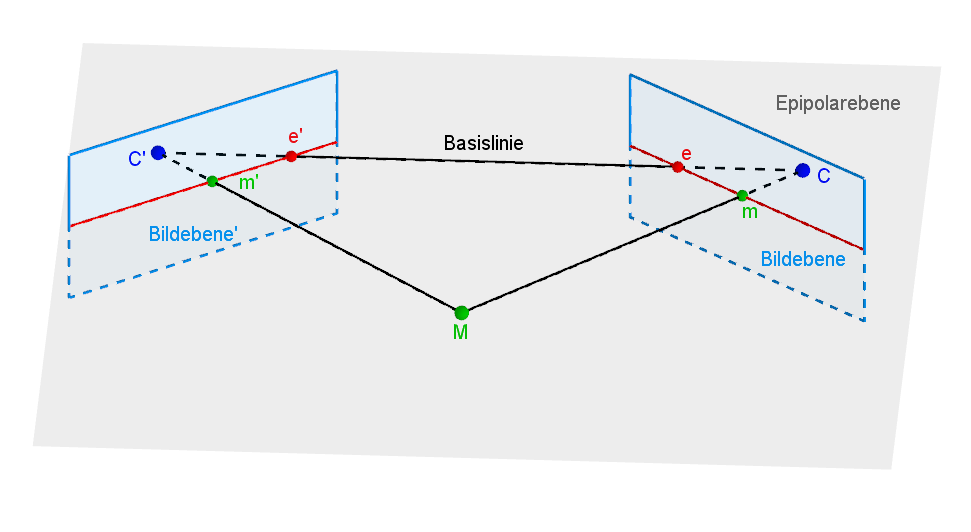
\includegraphics[width=1.\linewidth]{images/EpipolarGeoemtrieGrafik.png}
%	\captionof{figure}{Grafik zu den geometrischen Eigenschaften der Epipolargeometrie zwischen zweik Bildern. $C$ und $C'$ sind die Projektionszentren zweier Kameras. Beide Kameras besitzen jeweils eine Bildebene. Die Basislinien verbindet die Projektionszentren der Kameras. Der Punkt an welchem die Basislinie die Bildebenen schneidet, wird als Epipol bezeichnet. Durch den Epipol verlaufen alle Epipolarlinien des Bildes. $M$ ist der Objektpunkt im 3D-Raum und $m_1$ und $m_2$ sind die jeweiligen Abbildungen dieses Punktes auf den Bildebenen. Die Verbindungsvektoren zwischen $C, C'$ und $M$ bilden die sogenannte Epipolarebene\cite{Elements,HZ,ZZGXr}.}  
%\end{minipage}\\ \\
%
%
%Die Epipolarlinie $l'$, beinhaltet alle möglichen korrespondierenden Punkte zu $m$. Wenn $C$ auf seiner Bildebene $I$ einen Punkt $m$ abbildet, so erscheint dieser Punkt immer an der selben Stelle auf dem 2D - Bild, egal wie nah der Ursprüngliche 3D-Objektpunkt $M$ an $I$ befindet. Rein theoretisch, könnte der Originial Szenenpunkt $M$, sich überall auf der Verbindungslinie $\bar{Mm}$ befinden. Der Abgebildete Punkt $m$ wäre auf $I$ immer an der selben Stelle abgebildet. Fährt man nun mit $M$ die Verbindungslinie $\bar{Mm}$ entlang, dann ist $m$ immer an der selben Stelle auf $I$ zu sehen, während der korrespondierende Punkt $m'$ sich entlang der Epipolarlinie bewegen würde. Die Epipolargeometrie beschreibt also eine Beziehung zwischen einem Bildpunkt $m$ und dessen korrespondierender Epiplolarlinie $l'$, welche wiederum alle möglichen zu $m$ korrespondierenden Punkte $m'$ beinhaltet\cite{HZ,Zhang2014,ZZGXr}.\\
%
%
%
%\begin{minipage}{\linewidth}
%	\centering
%	\includegraphics[width=1.\linewidth]{images/EpipolarLinien.png}
%	\captionof{figure}{Die Objektpunkte $M_1, M_2$ und $M_3$ werden in $I'$ als $m'_1, m'_2$ und $m'_3$ abgebildet, während sie in $I$ immer den selben Bildpunkt $m_1$ ergeben.}  
%\end{minipage}\\ \\
%
%
%Die Epipolargeometrie lässt sich, ähnlich wie eines Homographiematrix, in einer 3x3-Matrix zusammenfassen. Diese ist jedoch singulär und besitzt somit nicht wie die Homographiematrix Rang 3 sondern Rang 2. Je nachdem ob ein ein kalibriertes oder unkalibriertes System vorliegen hat, handelt es sich entweder um die sogenannten Fundamental Matrix $F$ oder die Essentielle Matrix $E$ \cite{Elements,HZ,ZZPaper,Zhang2014,ZZGXr}. Von der Fundamentalmatrix $F$ ist dann die rede, wenn die intrinsischen Kameraparameter nicht bekannt sind, sprich wenn das System unkalibriert ist. In diesem Fall wird mit Bildpixelkoordinaten gearbeitet. Sind die intrinsischen Parameter bekannt, so wir $F$ zur essentiellen Matrix $E$ und es wird mit sogenannten normalisierten Bildkoordinaten gearbeitet\cite{ZZPaper}. Was genau die unterschiedlichen Koordinaten ausmacht, wird in Kapitel (KAPITELLINK) genauer erklärt. Mathematisch sagen die Matrizen $F$ und $E$ in Verbindung mit den korrespondierenden Punkten aus, ob für einen Bildpunkt $m$ in einer Kamera, dessen korrespondierender Bildpunkt $m'$ in der anderen Kamera auf der korrespondierenden Epipolarlinie liegt.  Das heißt, wenn $m'Fm = 0$ oder $\hat{m'}E\hat{m}= 0$, dann ist der sogenannte \textit{epipolar-constraint} erfüllt. Der \textit{epipolar-constraint} gibt somit Aufschluss darüber, ob $m'$ ein möglicher korrespondierender Punkt von $m$ ist. Dies ist nämlich genau dann der Fall, wenn $m'Fm = 0$ oder $\hat{m'}E\hat{m}= 0$ sind\cite{HZ,Zhang2014}. Ist der \textit{epipolar-constraint} erfüllt, so wird gleichzeitig der Suchaufwand nach weiteren Korrespondenzen reduziert, da somit nur noch eine eindimensionale Suche, entlang der Epipolarlinie, anstatt einer zweidimensionalen durchgeführt werden muss. Dieser neue \textit{contraint} wird auch als \textit{coplanarity constraint} oder Koplanaritätsbeschränkung bezeichnet. Dieser entsteht, da die Projektionszentren der Kameras und die korrespondierenden Bildpunkte auf ein und der selben Ebene liegen müssen \cite{Zhang2014}. Die Epipolargeometrie und die in ihr beinhalteten $constraints$, helfen bei der 3D-Szenenrekonstruktion. Szenenrekonstruktion ist dann möglich, wenn in einer Stereoaufnahme in beiden Bildern die zueinander gehörenden Bildpunkte lokalisiert wurden. Wird also eine Szene mit zwei Kameras aufgenommen, so liegen während der Aufnahme die aufgenommenen Objekpunkte, das Projektionszentrum und der zur Kamera gehörende Bildpunkt auf einer Linie. Wurde eine Objektpunkt nun zweimal aus verschiedenen Winkeln und/ oder Position aufgenommen, lassen sich nachdem die extrinsischen Parameter der Kameras ermittelt wurden, die Schnittpunkt der jeweiligen Linien aus Kamera eins und Kamera zwei berechnen. Diese Schnittpunkte ergeben den ursprünglichen Objektpunkt. Die Szene ist somit rekonstruiert\cite{Elements,ZZGXr,HZ}. 
%
%
%\section{Geometrische Erläuterung der Fundamentalmatrix und der Essentiellen Matrix }
%
%Nachdem die Theorie der geometrischen Hintergründe der Epipolargeometrie, bei der Stereokalibrierung und Szenerekonstruktion, erläutert wurden, wird nun der mathematische Hintergrund genauer aufgezeigt. Vor allem soll auf die Herleitung der neu eingeführten Fundamental Matrix $F$ und der essentiellen Matrix $E$ eingegangen werden. Diese spielen nämlich eine entscheidende Rolle bei der Rekonstruktion der Kamerapose und der Szenenrekonstruktion\cite{Elements, HZ}. $F$ und $E$ bilden jeweils eine singuläre 3x3-Matrix, welche die Geometrie zwischen den Bildpunkten $m_\tau$ und $m'_\tau$ auf $I$ und $I'$ und dem Objektpunkt $M_\delta$ im Raum beschreibt. Die Vektoren $\overline{CM} = (\vec{M}_\delta - \vec{C}_\delta),\, \overline{C'M} = (\vec{M}_\delta - \vec{C'}_\delta)$ und $\overline{CC'} = (\vec{C'}_\delta - \vec{C}_\delta)$ bilden das in Abbildung 3.12 sichtbare schwarze Dreieck. $F$ und $E$ fassen dieses Dreieck in ihren Matrizen zusammen. Um das ganze mathematisch zu erklären, wird ein Stereokameraufbau definiert. Ein Objektpunkt $M_\delta$ in Weltkoordinaten$(O,\delta)$ wird von zwei Kameras $C$ mit $(C,\beta)$ und $C'$ mit $(C',\beta')$ aufgenommen und auf deren Bildebenen $I$ und $I'$ als $m_\beta$ und $m'_\beta$ abgebildet. $C$ und $C'$ besitzen jeweils eine eigene Projektionsmatrix $P$ und $P'$. Anzumerken ist, dass die folgende Herleitung nach \cite{Elements} aufgestellt wurde.
%
%\begin{gather}
%	P = \begin{bmatrix}
%	KR|-KR\vec{C}_\delta
%	\end{bmatrix}\\
%	P' = \begin{bmatrix}
%	K'R'|-K'R'\vec{C'}_\delta
%	\end{bmatrix}
%\end{gather}
%
%$M$ wird mit $P$ und $P'$ auf die Bildebenen $I$ und $I'$ mit den jeweiligen Koordinatensystemen $I = (I,\tau)$ und $I'= (I',\tau')$ projiziert. Wichtig anzumerken, auch für den späteren Aufbau mit zwei Kameras unterschiedlicher Auflösung, ist, dass es sich bei den Koordinatensystemen von $I$ und $I'$ nicht um identische handeln muss.\cite{Elements} Es entstehen die Bildpunkte $\gamma m_\tau$ und $\gamma' m'_{\tau'}$ mit $\gamma \geq 0$ und $\gamma' \geq 0$. (gamma erklären)
%
%\begin{gather}
%	\gamma\vec{m}_\tau = P \begin{bmatrix}\vec{M}_\delta\\1\end{bmatrix}\\
%	\gamma\vec{m}_\tau = \begin{bmatrix}KR|-KR\vec{C}_\delta\end{bmatrix}\begin{bmatrix}\vec{M}_\delta\\1\end{bmatrix}\\
%	\gamma'\vec{m'}_{\tau'} = P' \begin{bmatrix}\vec{M}_\delta\\1\end{bmatrix}\\
%	\gamma'\vec{m'}_{\tau'} = \begin{bmatrix}K'R'|-K'R'\vec{C'}_\delta\end{bmatrix}\begin{bmatrix}\vec{M}_\delta\\1\end{bmatrix}\\
%\end{gather}
%
%$-KR\vec{C}_\delta$ und $-K'R'\vec{C'}_\delta$ verrechnet mit $M$ sind gleich den Vektorausdrücken $(\vec{M}_\delta - \vec{C}_\delta)$ und $(\vec{M}_\delta - \vec{C'}_\delta)$, welche die Verbindungslinie der beiden Projektionszentren mit dem Objektpunkt $M$ im Raum beschreiben.
%
%\begin{gather}
%	\gamma\vec{m}_\tau = KR(\vec{M}-\vec{C}_\delta)\\
%	\gamma'\vec{m'}_\tau = K'R'(\vec{M}-\vec{C'}_\delta)
%\end{gather}
%
%Gleichungen 3.89 und 3.90 werden nach $(\vec{M}-\vec{C}_\delta)$ und $(\vec{M}-\vec{C'}_\delta)$ aufgelöst.
%
%\begin{gather}
%	\gamma R^TK^{-1}\vec{m}_\tau = (\vec{M}-\vec{C}_\delta)\\
%	\gamma R'^TK'^{-1}\vec{m'}_{\tau'} = (\vec{M}-\vec{C'}_\delta)
%\end{gather}
%
%Wie bereits erwähnt ergibt sich aus den Vektoren $(\vec{M}_\delta - \vec{C}_\delta),\, (\vec{M}_\delta - \vec{C'}_\delta)$ und $(\vec{C'}_\delta - \vec{C}_\delta)$ das Dreieck aus Abbildung 3.12. Für das Dreieck kann, aus den drei Vektoren, die folgende Gleichung aufgestellt werden. 
%
%\begin{gather}
%	(\vec{C'}_\delta - \vec{C}_\delta) = (\vec{M}_\delta - \vec{C}_\delta) - (\vec{M}_\delta - \vec{C'}_\delta)
%\end{gather}
%
%$(\vec{M}-\vec{C}_\delta)$ und $(\vec{M} - \vec{C'}_\delta)$ können durch die Ausdrücke in den Gleichungen 3.91 und 3.92 ersetzt werden.
%
%\begin{gather}
%		(\vec{C'}_\delta - \vec{C}_\delta) = \gamma R^TK^{-1}\vec{m}_\tau - \gamma R'^TK'^{-1}\vec{m'}_{\tau'}
%\end{gather}
%
%Es gilt $\gamma \geq 0$ und $\gamma' \geq 0$, sie stehen für die Teife von $m$ und $m'$ und können mit Hilfe des Kreuzproduktes eliminiert werden\cite{Elements}. Zunächst wird $(\vec{C}'_\delta - \vec{C}_\delta)$ auf die rechte Seite gebracht, so dass die Gleichung nach Null aufgelöst wird.
%
%
%\begin{gather}
%	\begin{bmatrix}\vec{C'}_\delta - \vec{C}_\delta\end{bmatrix}_\times \gamma R^TK^{-1}\vec{m}_\tau - 
%	\begin{bmatrix}	\vec{C'}_\delta - \vec{C}_\delta\end{bmatrix}_\times \gamma' R'^TK'^{-1} \vec{m'}_{\tau'} =  0
%\end{gather}
%
%Gleichung 3.95 wird von links mit $\gamma' \vec{x'}^T_{\tau'}K'^{-T}R'$. Somit kann eine der beiden Schiefsymmetrischen Matrizen aus der Gleichung eliminiert werden. 
%
%\begin{gather}
%	\gamma' \vec{m'}_{\tau'} K'^{-T}R' \begin{bmatrix}	\vec{C'}_\delta - \vec{C}_\delta\end{bmatrix}_\times \gamma R^TK^{-1}\vec{m}_\tau = 0
%\end{gather}
%
%Da $\gamma \geq 0$ und $\gamma' \geq 0$, kann für Gleichung 3.96 auch folgendes geschrieben werden.
%
%\begin{gather}
%	 \vec{m'}_{\tau'} K'^{-T}R' \begin{bmatrix}	\vec{C'}_\delta - \vec{C}_\delta\end{bmatrix}_\times R^TK^{-1}\vec{m}_\tau = 0
%\end{gather}
%
%Aus Gleichung 3.97 können nun die Matrizen $F$ und $E$ ausgelesen werden. Bei $E$ handelt es sich um einen Kalibrierten Fall, dass bedeutet dass sowohl $K$ als auch $K'$ bekannt sind und die normalisierten Bildkoordinaten $\vec{\hat{m}}$ und $\vec{\hat{m}}'$  durch multiplikation mit $K$ und $K'$ entstehen. $E$ selbst fässt die Schiefsymmetrische Matrix $[\vec{C'}_\delta - \vec{C}_\delta]_\times$ und die beiden Transformationsmatrizen $R$ und $R'$ zusammen. 
%
%\begin{gather}
%	\vec{m'}_{\tau'}^T K'^{-T}EK^{-1}\vec{m}_\tau = 0\\
%	\vec{\hat{m}}_\tau^T E \vec{\hat{m}}'_{\tau'} = 0
%\end{gather}
%
%Matrix $E$ wird zu $F$, wenn es sich um einen unkalibrierten Fall handelt. Unkalibriert bedeutet, dass $K$ und $K'$ nicht bekannt sind, die Informationen zu $K$ und $K'$ in $F$ befinden. Werden $K$ und $K'$ zu $E'$ multipliziert, wird $E$ zu $F$. 
%
%\begin{gather}
%	\vec{m'}_{\tau'}^T K'^{-T}EK^{-1}\vec{m}_\tau = 0\\
%		\vec{m'}_{\tau'}^T F\vec{m}_\tau = 0
%\end{gather}
%
%$F$ und $E$, fassen die komplette Epipoloargeometrie, sprich externe und interne Parameter, sowie die geometrische Beziehung der jeweiligen Bildpunkte zu den 3-D Objektpunkten in einer 3x3-Matrix zusammen. Für $F$ und $E$ gibt es nicht nur eine Lösung. Werden $F$ oder $E$ Beispielsweise über den \textit{eight-Point-Algorithm} ermittelt, so sind die entstehenden 3x3-Matrixen und jedes vielfache von diesen gültige Lösungen für $F$ und $E$\cite{HZ,HZ8}. \textcolor{red}{Noch herausfinden ob das mit den Tiefen $\gamma$ und $\gamma'$ zusammenhängt!!}. Mit $F$ und $E$ kann wie bereits nachgeprüft werden, ob der \textit{epipolar-constraint} $m'^TFm = o$ oder $\hat{m'}^TE\hat{m} = 0$ zwischen zwei Bildpunkte gilt. Des weiteren können Epipole $e$ und $e'$ und Epipolarlinien $l$ und $l'$ ausfindig gemacht werden, sobald $E$ oder $F$ bekannt ist\cite{HZ,Elements,HZ8,ZZGXr}. Um die zu $m$ oder $m'$ korrespondierende Epipolarlinie $l'$ oder $l$ zu berechnen gilt:
%
%\begin{gather}
%l' = Fm\\
%l = F^Tm'
%\end{gather} 
%
%Um die Epipole $e$ und $e'$ zu berechnen die Gleichungen 3.103 und 3.104 erfüllt sein. Für $e$ reicht es also den rechten Nullraum von F zu bestimmen und für $e'$ muss dementsprechend der linke Nullraum von $F$ gefunden werden. 
%
%\begin{gather}
%	Fe = 0\\
%	F^Te' = 0
%\end{gather}
%
%Die Matrizen $F$ und $E$ sind die ausschlaggebenden Elemente, wenn es um die rekonstruktion der Kameraorientierungen und der Rekonstruktion der Szene geht. In beiden folgenden Kapitel werden zwei Beispiele zur Findung der exterenen Kameraparameter und der Szenenrekonstruktion aufgezeigt. Beim ersten Beispiel handelt es sich um ein Minimalbeispiel mit synthetisch erzeugten reinen Daten, um die theoretische Funktionalität des Algorithmus zu beweisen. Im zweiten Beispiel, wird der Algorithmus, mit einigen Anpassungen an die Realverhältnisse, auf Stereobildpaare, aufgenommen von zwei verschiedenen Kameras, angewandt. Die implementierten Algotithmen ermitteln aus einem Satz korrespondierender Bildpunkte die Fundamental Matrix und die essentielle Matrix mit Hilfe des sogenannten \textit{8-Point-Alhorithm}, Im Anschluss werden dann die externen Kameraparameter ermittelt und die Szene mit einem Triangulationsverfahren rekonstruiert. 
%

		
		
		\chapter{Epipolar Geometrie}


Die Epipolargeometrie beschreibt eine intrinsische projektive Geometrie zwischen zwei Bildern\cite{HZ}. Sie dient insbesondere zur Korrespondenzanalyse von Punkten aus Bildern und zur Gewinnung von 3-D-Informationen. Ohne Kenntnis der Kamerapositionen, kann mit Hilfe der Epipolargeometrie eine einfache Beziehung zwischen korrespondierenden Punkten hergestellt werden. Abbildung 3.12 zeigt, den Aufbau zweier Kameras mit ihren Projektionszentren $C$ und $C'$, deren Bildebenen $I$ und $I'$, welche vor den Projektionszentren platziert wurden. Die Bildebenen können sich auch hinter den Projektionszentren befinden, das hat letztendlich keinen Einfluss auf die geometrischen Beziehungen\cite{HZ}. Zu den Elementen der Epipolargeometrie gehören zum einen die Epipole $e$ und $e'$. Betrachtet man die Basislinie zwischen den beiden Projektionszentren, so entsteht der Epipol genau am Schnittpunkt der Verbindungslinie mit den jeweiligen Bildebenen. Tritt der Fall ein, dass die Basislinie parallel zu einer oder beiden Bildebenen ist, so kommt es zu keiner Abbildung des Epipols auf den entsprechenden Bildebenen, sondern der Epipol befindet sich in diesem Falle im unendlichen\cite{ZZGXr}. Das hat zur Folge, dass alle Epipolarlinien, welche durch den Epipol verlaufen, sich zueinander parallel anordnen. Epipolarlinien die Linien, welche durch einen Bildpunkt $m$ oder $m'$ und dem jeweiligen Epipol $e$ oder $e'$ des Bildes verlaufen. Der Korrespondierende Punkt zu $m$ ist $m'$ und die korrespondierende Epipolarlinie $l'$ zu $m$, ist diejenige Linie, welche durch $m'$ und $e'$ verläuft. 


\begin{minipage}{\linewidth}
	\centering
	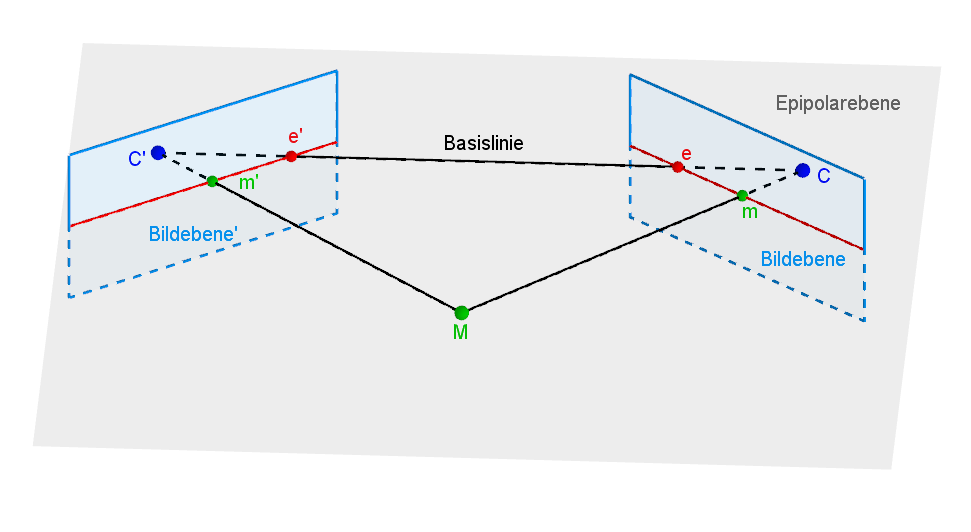
\includegraphics[width=1.\linewidth]{images/EpipolarGeoemtrieGrafik.png}
	\captionof{figure}{Grafik zu den geometrischen Eigenschaften der Epipolargeometrie zwischen zweik Bildern. $C$ und $C'$ sind die Projektionszentren zweier Kameras. Beide Kameras besitzen jeweils eine Bildebene. Die Basislinien verbindet die Projektionszentren der Kameras. Der Punkt an welchem die Basislinie die Bildebenen schneidet, wird als Epipol bezeichnet. Durch den Epipol verlaufen alle Epipolarlinien des Bildes. $M$ ist der Objektpunkt im 3D-Raum und $m_1$ und $m_2$ sind die jeweiligen Abbildungen dieses Punktes auf den Bildebenen. Die Verbindungsvektoren zwischen $C, C'$ und $M$ bilden die sogenannte Epipolarebene\cite{Elements,HZ,ZZGXr}.}  
\end{minipage}\\ \\


Die Epipolarlinie $l'$, beinhaltet alle möglichen korrespondierenden Punkte zu $m$. Wenn $C$ auf seiner Bildebene $I$ einen Punkt $m$ abbildet, so erscheint dieser Punkt immer an der selben Stelle auf dem 2D - Bild, egal wie nah der Ursprüngliche 3D-Objektpunkt $M$ an $I$ befindet. Rein theoretisch, könnte der Originial Szenenpunkt $M$, sich überall auf der Verbindungslinie $\bar{Mm}$ befinden. Der Abgebildete Punkt $m$ wäre auf $I$ immer an der selben Stelle abgebildet. Fährt man nun mit $M$ die Verbindungslinie $\bar{Mm}$ entlang, dann ist $m$ immer an der selben Stelle auf $I$ zu sehen, während der korrespondierende Punkt $m'$ sich entlang der Epipolarlinie bewegen würde. Die Epipolargeometrie beschreibt also eine Beziehung zwischen einem Bildpunkt $m$ und dessen korrespondierender Epiplolarlinie $l'$, welche wiederum alle möglichen zu $m$ korrespondierenden Punkte $m'$ beinhaltet\cite{HZ,Zhang2014,ZZGXr}.\\



\begin{minipage}{\linewidth}
	\centering
	\includegraphics[width=1.\linewidth]{images/EpipolarLinien.png}
	\captionof{figure}{Die Objektpunkte $M_1, M_2$ und $M_3$ werden in $I'$ als $m'_1, m'_2$ und $m'_3$ abgebildet, während sie in $I$ immer den selben Bildpunkt $m_1$ ergeben.}  
\end{minipage}\\ \\


Die Epipolargeometrie lässt sich, ähnlich wie eines Homographiematrix, in einer 3x3-Matrix zusammenfassen. Diese ist jedoch singulär und besitzt somit nicht wie die Homographiematrix Rang 3 sondern Rang 2. Je nachdem ob ein ein kalibriertes oder unkalibriertes System vorliegen hat, handelt es sich entweder um die sogenannten Fundamental Matrix $F$ oder die Essentielle Matrix $E$ \cite{Elements,HZ,ZZPaper,Zhang2014,ZZGXr}. Von der Fundamentalmatrix $F$ ist dann die rede, wenn die intrinsischen Kameraparameter nicht bekannt sind, sprich wenn das System unkalibriert ist. In diesem Fall wird mit Bildpixelkoordinaten gearbeitet. Sind die intrinsischen Parameter bekannt, so wir $F$ zur essentiellen Matrix $E$ und es wird mit sogenannten normalisierten Bildkoordinaten gearbeitet\cite{ZZPaper}. Was genau die unterschiedlichen Koordinaten ausmacht, wird in Kapitel (KAPITELLINK) genauer erklärt. Mathematisch sagen die Matrizen $F$ und $E$ in Verbindung mit den korrespondierenden Punkten aus, ob für einen Bildpunkt $m$ in einer Kamera, dessen korrespondierender Bildpunkt $m'$ in der anderen Kamera auf der korrespondierenden Epipolarlinie liegt.  Das heißt, wenn $m'Fm = 0$ oder $\hat{m'}E\hat{m}= 0$, dann ist der sogenannte \textit{epipolar-constraint} erfüllt. Der \textit{epipolar-constraint} gibt somit Aufschluss darüber, ob $m'$ ein möglicher korrespondierender Punkt von $m$ ist. Dies ist nämlich genau dann der Fall, wenn $m'Fm = 0$ oder $\hat{m'}E\hat{m}= 0$ sind\cite{HZ,Zhang2014}. Ist der \textit{epipolar-constraint} erfüllt, so wird gleichzeitig der Suchaufwand nach weiteren Korrespondenzen reduziert, da somit nur noch eine eindimensionale Suche, entlang der Epipolarlinie, anstatt einer zweidimensionalen durchgeführt werden muss. Dieser neue \textit{contraint} wird auch als \textit{coplanarity constraint} oder Koplanaritätsbeschränkung bezeichnet. Dieser entsteht, da die Projektionszentren der Kameras und die korrespondierenden Bildpunkte auf ein und der selben Ebene liegen müssen \cite{Zhang2014}. Die Epipolargeometrie und die in ihr beinhalteten $constraints$, helfen bei der 3D-Szenenrekonstruktion. Szenenrekonstruktion ist dann möglich, wenn in einer Stereoaufnahme in beiden Bildern die zueinander gehörenden Bildpunkte lokalisiert wurden. Wird also eine Szene mit zwei Kameras aufgenommen, so liegen während der Aufnahme die aufgenommenen Objekpunkte, das Projektionszentrum und der zur Kamera gehörende Bildpunkt auf einer Linie. Wurde eine Objektpunkt nun zweimal aus verschiedenen Winkeln und/ oder Position aufgenommen, lassen sich nachdem die extrinsischen Parameter der Kameras ermittelt wurden, die Schnittpunkt der jeweiligen Linien aus Kamera eins und Kamera zwei berechnen. Diese Schnittpunkte ergeben den ursprünglichen Objektpunkt. Die Szene ist somit rekonstruiert\cite{Elements,ZZGXr,HZ}. 


\section{Geometrische Erläuterung der Fundamentalmatrix und der Essentiellen Matrix }

Nachdem die Theorie der geometrischen Hintergründe der Epipolargeometrie, bei der Stereokalibrierung und Szenerekonstruktion, erläutert wurden, wird nun der mathematische Hintergrund genauer aufgezeigt. Vor allem soll auf die Herleitung der neu eingeführten Fundamental Matrix $F$ und der essentiellen Matrix $E$ eingegangen werden. Diese spielen nämlich eine entscheidende Rolle bei der Rekonstruktion der Kamerapose und der Szenenrekonstruktion\cite{Elements, HZ}. $F$ und $E$ bilden jeweils eine singuläre 3x3-Matrix, welche die Geometrie zwischen den Bildpunkten $m_\tau$ und $m'_\tau$ auf $I$ und $I'$ und dem Objektpunkt $M_\delta$ im Raum beschreibt. Die Vektoren $\overline{CM} = (\vec{M}_\delta - \vec{C}_\delta),\, \overline{C'M} = (\vec{M}_\delta - \vec{C'}_\delta)$ und $\overline{CC'} = (\vec{C'}_\delta - \vec{C}_\delta)$ bilden das in Abbildung 3.12 sichtbare schwarze Dreieck. $F$ und $E$ fassen dieses Dreieck in ihren Matrizen zusammen. Um das ganze mathematisch zu erklären, wird ein Stereokameraufbau definiert. Ein Objektpunkt $M_\delta$ in Weltkoordinaten$(O,\delta)$ wird von zwei Kameras $C$ mit $(C,\beta)$ und $C'$ mit $(C',\beta')$ aufgenommen und auf deren Bildebenen $I$ und $I'$ als $m_\beta$ und $m'_\beta$ abgebildet. $C$ und $C'$ besitzen jeweils eine eigene Projektionsmatrix $P$ und $P'$. Anzumerken ist, dass die folgende Herleitung nach \cite{Elements} aufgestellt wurde.

\begin{gather}
P = \begin{bmatrix}
KR|-KR\vec{C}_\delta
\end{bmatrix}\\
P' = \begin{bmatrix}
K'R'|-K'R'\vec{C'}_\delta
\end{bmatrix}
\end{gather}

$M$ wird mit $P$ und $P'$ auf die Bildebenen $I$ und $I'$ mit den jeweiligen Koordinatensystemen $I = (I,\tau)$ und $I'= (I',\tau')$ projiziert. Wichtig anzumerken, auch für den späteren Aufbau mit zwei Kameras unterschiedlicher Auflösung, ist, dass es sich bei den Koordinatensystemen von $I$ und $I'$ nicht um identische handeln muss.\cite{Elements} Es entstehen die Bildpunkte $\gamma m_\tau$ und $\gamma' m'_{\tau'}$ mit $\gamma \geq 0$ und $\gamma' \geq 0$. (gamma erklären)

\begin{gather}
\gamma\vec{m}_\tau = P \begin{bmatrix}\vec{M}_\delta\\1\end{bmatrix}\\
\gamma\vec{m}_\tau = \begin{bmatrix}KR|-KR\vec{C}_\delta\end{bmatrix}\begin{bmatrix}\vec{M}_\delta\\1\end{bmatrix}\\
\gamma'\vec{m'}_{\tau'} = P' \begin{bmatrix}\vec{M}_\delta\\1\end{bmatrix}\\
\gamma'\vec{m'}_{\tau'} = \begin{bmatrix}K'R'|-K'R'\vec{C'}_\delta\end{bmatrix}\begin{bmatrix}\vec{M}_\delta\\1\end{bmatrix}\\
\end{gather}

$-KR\vec{C}_\delta$ und $-K'R'\vec{C'}_\delta$ verrechnet mit $M$ sind gleich den Vektorausdrücken $(\vec{M}_\delta - \vec{C}_\delta)$ und $(\vec{M}_\delta - \vec{C'}_\delta)$, welche die Verbindungslinie der beiden Projektionszentren mit dem Objektpunkt $M$ im Raum beschreiben.

\begin{gather}
\gamma\vec{m}_\tau = KR(\vec{M}-\vec{C}_\delta)\\
\gamma'\vec{m'}_\tau = K'R'(\vec{M}-\vec{C'}_\delta)
\end{gather}

Gleichungen 3.89 und 3.90 werden nach $(\vec{M}-\vec{C}_\delta)$ und $(\vec{M}-\vec{C'}_\delta)$ aufgelöst.

\begin{gather}
\gamma R^TK^{-1}\vec{m}_\tau = (\vec{M}-\vec{C}_\delta)\\
\gamma R'^TK'^{-1}\vec{m'}_{\tau'} = (\vec{M}-\vec{C'}_\delta)
\end{gather}

Wie bereits erwähnt ergibt sich aus den Vektoren $(\vec{M}_\delta - \vec{C}_\delta),\, (\vec{M}_\delta - \vec{C'}_\delta)$ und $(\vec{C'}_\delta - \vec{C}_\delta)$ das Dreieck aus Abbildung 3.12. Für das Dreieck kann, aus den drei Vektoren, die folgende Gleichung aufgestellt werden. 

\begin{gather}
(\vec{C'}_\delta - \vec{C}_\delta) = (\vec{M}_\delta - \vec{C}_\delta) - (\vec{M}_\delta - \vec{C'}_\delta)
\end{gather}

$(\vec{M}-\vec{C}_\delta)$ und $(\vec{M} - \vec{C'}_\delta)$ können durch die Ausdrücke in den Gleichungen 3.91 und 3.92 ersetzt werden.

\begin{gather}
(\vec{C'}_\delta - \vec{C}_\delta) = \gamma R^TK^{-1}\vec{m}_\tau - \gamma R'^TK'^{-1}\vec{m'}_{\tau'}
\end{gather}

Es gilt $\gamma \geq 0$ und $\gamma' \geq 0$, sie stehen für die Teife von $m$ und $m'$ und können mit Hilfe des Kreuzproduktes eliminiert werden\cite{Elements}. Zunächst wird $(\vec{C}'_\delta - \vec{C}_\delta)$ auf die rechte Seite gebracht, so dass die Gleichung nach Null aufgelöst wird.


\begin{gather}
\begin{bmatrix}\vec{C'}_\delta - \vec{C}_\delta\end{bmatrix}_\times \gamma R^TK^{-1}\vec{m}_\tau - 
\begin{bmatrix}	\vec{C'}_\delta - \vec{C}_\delta\end{bmatrix}_\times \gamma' R'^TK'^{-1} \vec{m'}_{\tau'} =  0
\end{gather}

Gleichung 3.95 wird von links mit $\gamma' \vec{x'}^T_{\tau'}K'^{-T}R'$. Somit kann eine der beiden Schiefsymmetrischen Matrizen aus der Gleichung eliminiert werden. 

\begin{gather}
\gamma' \vec{m'}_{\tau'} K'^{-T}R' \begin{bmatrix}	\vec{C'}_\delta - \vec{C}_\delta\end{bmatrix}_\times \gamma R^TK^{-1}\vec{m}_\tau = 0
\end{gather}

Da $\gamma \geq 0$ und $\gamma' \geq 0$, kann für Gleichung 3.96 auch folgendes geschrieben werden.

\begin{gather}
\vec{m'}_{\tau'} K'^{-T}R' \begin{bmatrix}	\vec{C'}_\delta - \vec{C}_\delta\end{bmatrix}_\times R^TK^{-1}\vec{m}_\tau = 0
\end{gather}

Aus Gleichung 3.97 können nun die Matrizen $F$ und $E$ ausgelesen werden. Bei $E$ handelt es sich um einen Kalibrierten Fall, dass bedeutet dass sowohl $K$ als auch $K'$ bekannt sind und die normalisierten Bildkoordinaten $\vec{\hat{m}}$ und $\vec{\hat{m}}'$  durch multiplikation mit $K$ und $K'$ entstehen. $E$ selbst fässt die Schiefsymmetrische Matrix $[\vec{C'}_\delta - \vec{C}_\delta]_\times$ und die beiden Transformationsmatrizen $R$ und $R'$ zusammen. 

\begin{gather}
\vec{m'}_{\tau'}^T K'^{-T}EK^{-1}\vec{m}_\tau = 0\\
\vec{\hat{m}}_\tau^T E \vec{\hat{m}}'_{\tau'} = 0
\end{gather}

Matrix $E$ wird zu $F$, wenn es sich um einen unkalibrierten Fall handelt. Unkalibriert bedeutet, dass $K$ und $K'$ nicht bekannt sind, die Informationen zu $K$ und $K'$ in $F$ befinden. Werden $K$ und $K'$ zu $E'$ multipliziert, wird $E$ zu $F$. 

\begin{gather}
\vec{m'}_{\tau'}^T K'^{-T}EK^{-1}\vec{m}_\tau = 0\\
\vec{m'}_{\tau'}^T F\vec{m}_\tau = 0
\end{gather}

$F$ und $E$, fassen die komplette Epipoloargeometrie, sprich externe und interne Parameter, sowie die geometrische Beziehung der jeweiligen Bildpunkte zu den 3-D Objektpunkten in einer 3x3-Matrix zusammen. Für $F$ und $E$ gibt es nicht nur eine Lösung. Werden $F$ oder $E$ Beispielsweise über den \textit{eight-Point-Algorithm} ermittelt, so sind die entstehenden 3x3-Matrixen und jedes vielfache von diesen gültige Lösungen für $F$ und $E$\cite{HZ,HZ8}. \textcolor{red}{Noch herausfinden ob das mit den Tiefen $\gamma$ und $\gamma'$ zusammenhängt!!}. Mit $F$ und $E$ kann wie bereits nachgeprüft werden, ob der \textit{epipolar-constraint} $m'^TFm = o$ oder $\hat{m'}^TE\hat{m} = 0$ zwischen zwei Bildpunkte gilt. Des weiteren können Epipole $e$ und $e'$ und Epipolarlinien $l$ und $l'$ ausfindig gemacht werden, sobald $E$ oder $F$ bekannt ist\cite{HZ,Elements,HZ8,ZZGXr}. Um die zu $m$ oder $m'$ korrespondierende Epipolarlinie $l'$ oder $l$ zu berechnen gilt:

\begin{gather}
l' = Fm\\
l = F^Tm'
\end{gather} 

Um die Epipole $e$ und $e'$ zu berechnen die Gleichungen 3.103 und 3.104 erfüllt sein. Für $e$ reicht es also den rechten Nullraum von F zu bestimmen und für $e'$ muss dementsprechend der linke Nullraum von $F$ gefunden werden. 

\begin{gather}
Fe = 0\\
F^Te' = 0
\end{gather}

Die Matrizen $F$ und $E$ sind die ausschlaggebenden Elemente, wenn es um die rekonstruktion der Kameraorientierungen und der Rekonstruktion der Szene geht. In beiden folgenden Kapitel werden zwei Beispiele zur Findung der exterenen Kameraparameter und der Szenenrekonstruktion aufgezeigt. Beim ersten Beispiel handelt es sich um ein Minimalbeispiel mit synthetisch erzeugten reinen Daten, um die theoretische Funktionalität des Algorithmus zu beweisen. Im zweiten Beispiel, wird der Algorithmus, mit einigen Anpassungen an die Realverhältnisse, auf Stereobildpaare, aufgenommen von zwei verschiedenen Kameras, angewandt. Die implementierten Algotithmen ermitteln aus einem Satz korrespondierender Bildpunkte die Fundamental Matrix und die essentielle Matrix mit Hilfe des sogenannten \textit{8-Point-Alhorithm}, Im Anschluss werden dann die externen Kameraparameter ermittelt und die Szene mit einem Triangulationsverfahren rekonstruiert. 


		
		% C1 - example 3
		\chapter{Synthetische Rekonstruktion}
\label{sec:minimal} 

Anhand der erarbeiteten mathematischen Grundlagen ist ein Algorithmus für die Rekonstruktion einer Szene aus einer Stereobildaufnahme entstanden. Der Algorithmus wurde mit dem Ziel der Kamerakalibrierung und der Szenenrekonstruktion aus Bildquellen unterschiedlicher Auflösungen entwickelt, da Stereokalibrierungsverfahren einiger Computer Vision Applikationen keine unterschiedlichen Auflösungen von Kameras berücksichtigen. Der entwickelte Algorithmus ist in der Lage aus einem Stereobildpaar extrinsische Kameraparameter zu bestimmen und anhand dessen die 3D-Szene zu rekonstruieren, jedoch unter der Voraussetzung, dass die intrinsischen Kameraparameter beider Kameras bekannt sind.\\

Im Folgenden wird der Algorithmus anhand eines virtuellen Beispiels erklärt. Dabei werden die einzelnen Schritte des Aufbaus der virtuellen Szene, der Bestimmung der extrinsischen Kameraparameter und der Rekonstruktion der virtuellen 3D-Szene beschrieben. Abbildung \ref{fig:ArbeitsProzessVirtuell} fasst den Arbeitsprozess des Szenenrekonstruktionsalgorithmus für das virtuelle Beispiel zusammen. \\




\begin{figure}[!htb]%{\linewidth}
	\centering
	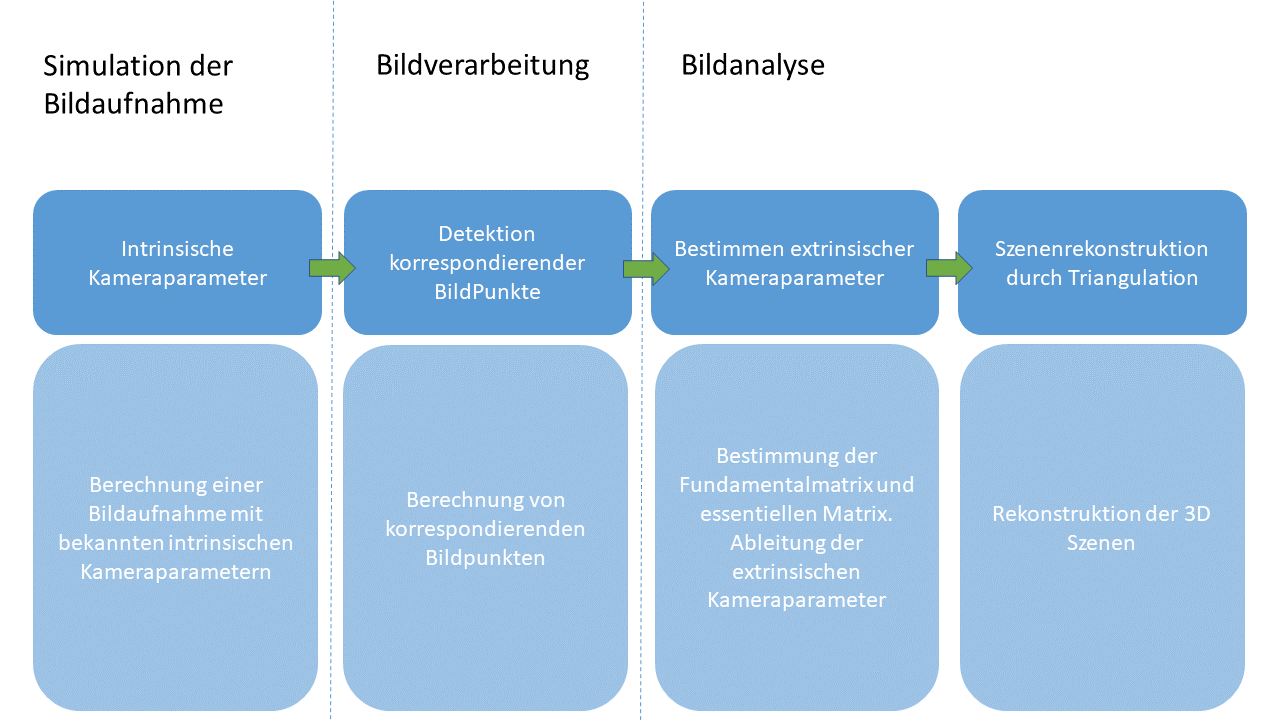
\includegraphics[width=1.\linewidth]{images/NEU_Virtuel_Arbeitsprozess.png}
	\caption[Ablaufdiagram]{Ablaufdiagramm für das synthetische Beispiel}
	\label{fig:ArbeitsProzessVirtuell}
\end{figure}

%\begin{figure}%{\linewidth}
%	\centering
%	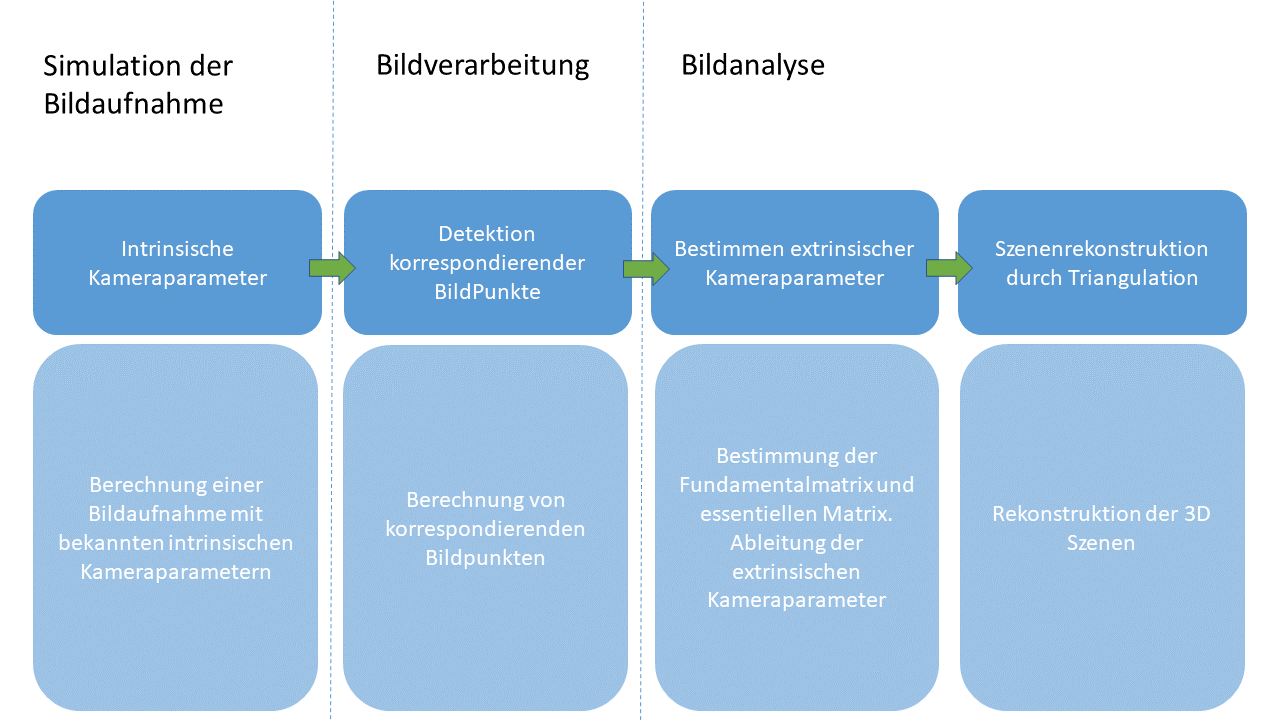
\includegraphics[width=0.8\linewidth]{images/NEU_Virtuel_Arbeitsprozess.png}
%	\caption[Ablaufdiagram]{Ablaufdiagramm für das synthetische Beispiel}
%	\label{fig:ArbeitsProzessVirtuell}
%\end{figure}
\pagebreak

%
%Für die Entwicklung des Ansatzes für den Szenenrekonstruktionsalgorithmus sind  des Algorithmus sind 



\section{Simulierte Bildaufnahme einer virtuellen Szene}

Als 3D-Objekt wurde ein Quader, in ein Weltkoordinatensystem $(O,\delta)$ mit $\delta = (\hat{d_1},\hat{d_2},\hat{d_3})$ positioniert. Es werden zwei Kameras $(C,\beta)$ mit $\beta = (\hat{b_1},\hat{b_2},\hat{b_3})$ und $(C',\beta')$ mit $\beta' = (\hat{b'_1},\hat{b'_2},\hat{b'_3})$ in $(O,\delta)$ platziert. Das Weltkoordinatensystem $(O,\delta)$ und das Kamerakoordinatensystem $(C,\beta)$ sind deckungsgleich. $C'$ ist relativ zu $C$ verschoben und rotiert. Die zwei Bildebenen $(I,\tau)$ mit $\tau = (\hat{t_1},\hat{t_2},\hat{t_3})$ und $(I',\tau')$ mit $\tau' = (\hat{t_1}',\hat{t_2}',\hat{t_3}')$ sind vor $C$ und $C'$ positioniert. Die Sensorkoordinatensysteme $(S,\sigma)$ und $(S',\sigma')$ wurden gleich den Bildebenenkoordinatensystemen $(I,\tau)$ und $(I',\tau')$ gesetzt. Es wird von zwei identischen Kameras ausgegangen und somit werden für den hier diskutierten Fall ausschließlich mit dem vereinfachten Kameramatrizen $K_0$ gerechnet. Der schematische Aufbau der Szenen ist in den Abbildungen \ref{fig:aufbauMinimalTopDown}, \ref{fig:AbbildungenMinimal} und \ref{fig:KoordsystemeMinimal} dargestellt.

%Somit reicht für das synthetische Beispiel die vereinfachten Kameramatrix $K_0$, wie in Kapitel \ref{sec:CameraModels} definiert, aus.


%Kamera eins $(C,\beta)$ ist Deckungsgleich mit $(O,\delta)$. Kamera zwei $(C',\beta')$ wurde von $C$ in positive $d_1$-Richtung, verschoben und um einen Winkel $\alpha$ zu $C$ um die eigene $b'_3$-Achse rotiert. Die verwendeten kartesischen Koordinatensysteme sind in diesem Minimalbeispiel alle rechtshändig orientiert. Die äußeren und inneren Kameraparameter wurden für den Aufbau der Szene festgelegt. Dies hat den positiven Effekt, dass somit die späteren Ergebnisse besser validiert werden können. In den Abbildung \ref{fig:aufbauMinimalTopDown} bis \ref{fig:KoordsystemeMinimal} wird der Aufbau noch einmal genauer veranschaulicht. \\

\begin{figure}[!htb]
	\minipage{0.52\textwidth}
	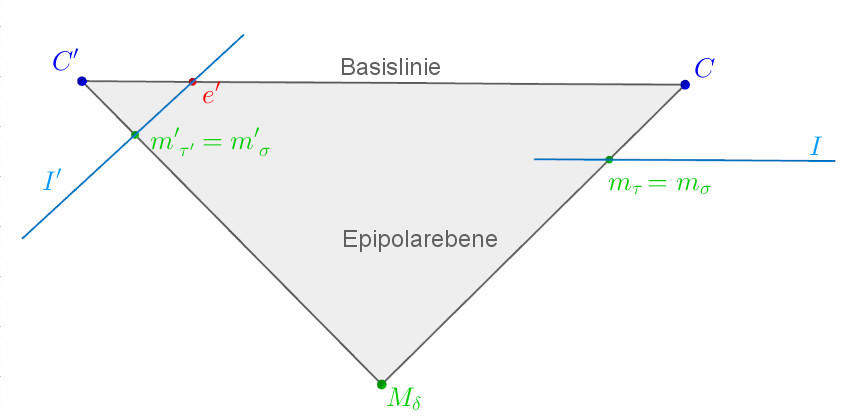
\includegraphics[width=\linewidth]{images/SynthetischesBeispielAufbauTopDown_beschriftet.png}
	\caption[Synthetisches Beispiel Top-Down-Ansicht]{In der Abbildung ist der vereinfachte Stereoaufbau in einer Top-Down-Ansicht zu sehen}
	\label{fig:aufbauMinimalTopDown}
	\endminipage\hfill
	\minipage{0.42\textwidth}
	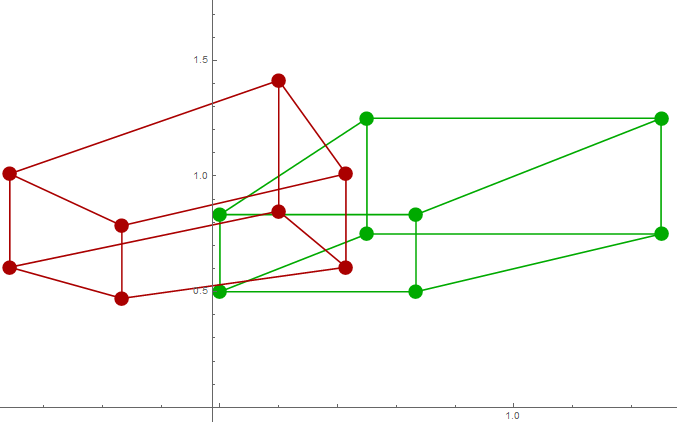
\includegraphics[width=\linewidth]{images/QuadrateMinimalBeispiel.png}
	\caption[Simulierte Abbildung eines Quaders auf zwei Kameras]{Simulierite Abbildung des Quaders auf die Kamera $C$ in Grün und auf $C'$ in Rot}
	\label{fig:AbbildungenMinimal}
	\endminipage\hfill
\end{figure}

\begin{figure}[!htb]
	\centering
	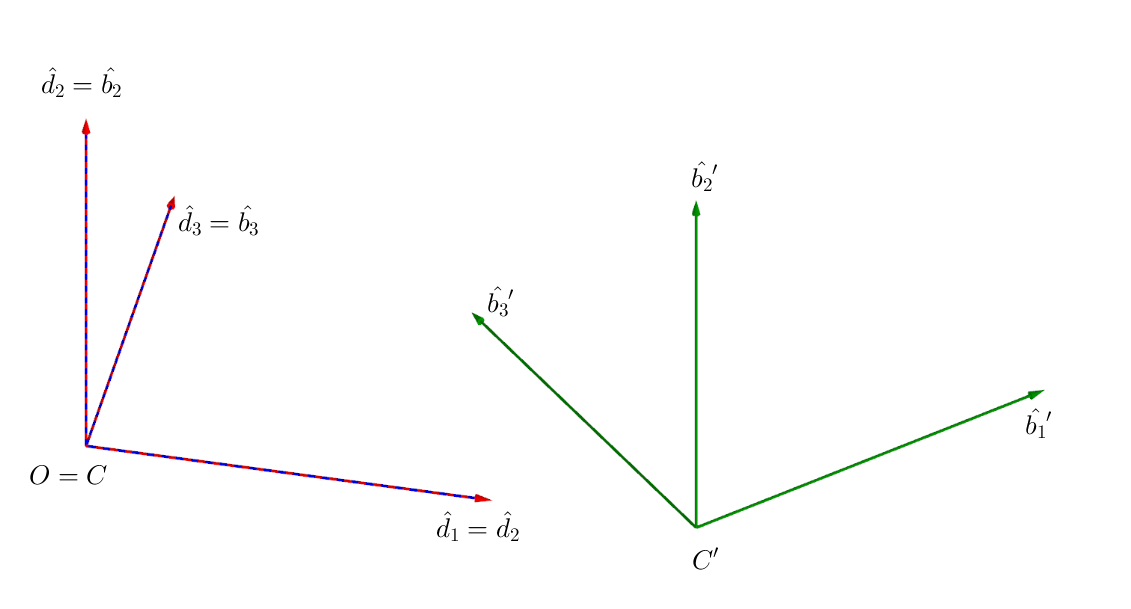
\includegraphics[width=.6\linewidth]{images/KS_Minimalbeispiel_beschriftet.png}
	\caption[Koordinatensysteme von $C$ und $C'$]{Abbildung der verschiedenen Kamerakoordinatensysteme, das Weltkoordinatensystem  $O$ ist zum Kamerakoordinatensystem $C$ deckungsgleich und $C'$  verschoben und rotiert.}
	\label{fig:KoordsystemeMinimal}
\end{figure}

%\begin{minipage}{\linewidth}
%	\centering
%	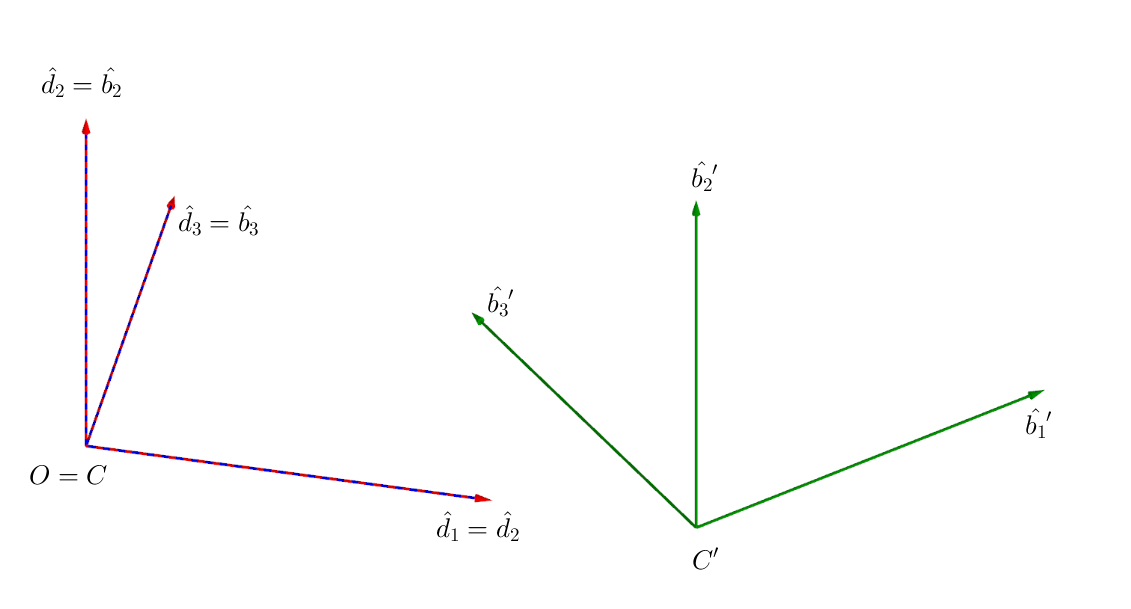
\includegraphics[width=.6\linewidth]{images/KS_Minimalbeispiel_beschriftet.png}
%	\captionof{figure}{Abbildung der verschiedenen Kamerakoordinatensysteme, das Weltkoordinatensystem  $O$ ist zum Kamerakoordinatensystem $C$ deckungsgleich und $C'$  verschoben und rotiert.}
%	\label{fig:KoordsystemeMinimal}
%\end{minipage}\\ \\

%
%Für die Stereokamerakalibrierung wird $C'$ relativ zur zu $C$ um einen Vektor \ensuremath{\vec{V'}} verschoben und anschließend um einen Winkel \ensuremath{\alpha} um die $b'_3$ Achse gedreht. Für die Rotation um \ensuremath{b'_3} wird eine Drehmatrix $D'$ aufgestellt.
Um die Eckpunkte des Quaders auf die Bildebenen von $C$ und $C'$ abbilden zu können, werden zunächst die Projektionsmatrizen $P$ und $P'$ aufgestellt. $C$ ist deckungsgleich mit dem Weltkoordinatensystem $(O,\delta)$. Es gilt also

\begin{gather}
R=\begin{pmatrix}
1&0&0\\
0&1&0\\
0&0&1
\end{pmatrix}\\
C=\begin{pmatrix}
0\\0\\0
\end{pmatrix}\\
T = R[I|-C]\\
T = \begin{bmatrix}
1&&0&&0&&C_1\\
0&&1&&0&&C_2\\
0&&0&&1&&C_3
\end{bmatrix}
\end{gather}. 

$C'$ dagegen ist gegenüber $C$ verschoben und rotiert. Als Beispiel wird eine Rotation um die $\hat{b_2}'$ Achse für $C'$ bestimmt. Somit gilt für $P'$:
%entlang $\hat{d_1}$ verschoben und um $\hat{b_2}$ rotiert. Somit ergibt sich für $T=[R|V]$ von $C$:

%Dabei gehen wir davon aus, dass $C$ weder rotiert noch verschoben ist, während $C'$ verschoben und rotiert ist.(Hier eher wieder allgemein bleiben C gegenüber O keine verönderung C' schon)





%Die entstandene Matrix \ensuremath{R'} beschreibt die Transformation $C'$ und somit auch die Transformation von Punkten des Koordinatensystems $(C,\beta)$ in $(C',\beta')$. Da $(C,\beta) = (O,\delta)$ ist, beinhaltet die Transformationsmatrix $R$ für $C$ weder eine Translation noch eine Rotation.

%Und für $R'=[D'|V']$ von $C'$ gilt:

\begin{gather}			
	R'= 
	\begin{pmatrix}
		\cos(\alpha)&0&\sin(\alpha)\\
		0&1&0\\
		-\sin(\alpha)&0&\cos(\alpha)
	\end{pmatrix}\\
	\vec{C'}= 
	\begin{pmatrix}
		1&0&0&-C'_1\\
		0&1&0&-C'_2\\
		0&0&1&-C'_3			
	\end{pmatrix}\\
	T'=R'[I|-C]\\
	T'=		\begin{pmatrix}
		\cos(\alpha)&0&-\sin(\alpha)\\
		0&1&0\\
		\sin(\alpha)&0&\cos(\alpha)
	\end{pmatrix} 
	\cdot
	\begin{pmatrix}
		1&0&0&-C'_1\\
		0&1&0&-C'_2\\
		0&0&1&-C'_3			
	\end{pmatrix}\\
	T'=
	\begin{pmatrix}
		\cos(\alpha)&0&-\sin(\alpha)&-C'_1\cos(\alpha)+C'_3\sin(\alpha)\\
		0&1&0&-C'_2\\
		\sin(\alpha)&0&\cos(\alpha)&-C'_1\sin(\alpha)-C'_3\cos(\alpha)\\
	\end{pmatrix}
\end{gather}\\

%\section{Berechnung der Projetkionsmatritzen }

%Neben den Eckpunkten des Quaders wird noch ein neunter Punkt $E_\delta$ außerhalb des Quaders platziert und zwar so, dass es zu keinen linearen Abhängigkeiten zwischen $E_\delta$ und den anderen Punkten kommt. 


Der Quader hat insgesamt acht Punkte, welche auf die Bildebenen der Kameras projiziert werden. Neben den Punkte des Quaders wird noch ein weiterer Punkt außerhalb des Quaders platziert und ebenfalls auf die Bildebenen projiziert. Mit insgesamt neun Punkten bei der Bestimmung der Fundamentalmatrix, wird die Wahrscheinlichkeit ein unterbestimmtes System aus der Koeffizientenmatrix $A$ zu bekommen minimiert. Ist $A$ unterbestimmt so besitzt sie Rang 7 und $F$ kann nicht eindeutig durch einen Sieben-Punkte-Algorithmus bestimmt werden\cite{HZ,LongQuan}. In dem hier berechneten Beispiel werden deswegen neun Punkte benutzt um sicherzugehen, dass $A$ Rang 8 besitzt und somit eindeutig bestimmt werden kann. Zur Bestimmung von $F$, wird der in Kapitel \ref{sec:HFE} aufgeführte Acht-Punkte Algorithmus angewandt.\\



%Mit insgesamt neun Punkten bei der Bestimmung der Fundamentalmatrix wird das Risiko einen Rangverlust durch lineare Abhängigkeiten minimiert\cite{HZ}. In Kapitel \ref{fig:Homographie} wurde geschildert, dass wenn die Koeffizientenmatrix $A$ einen Rang $\geq 8$ aufweist, $F$ mit Hilfe der Singulärwertzerlegung bestimmt werden kann\cite{HZ,Schwarz}. Besitz $A$ einen Rang von 7, so entspricht $A$ einer 7 $\times$ 9-Matrix. $A$ verhält sich wie eine Matrix, welche aus 7 statt 8 oder mehr Punktekorrespondenzen aufgestellt wurde. Das Verfahren die Fundamentalmatrix aus $A$ mit Rang 7 zu bestimmen, wird als der Sieben-Punkt-Algorithmus bezeichnet\cite{HZ,LongQuan}. In diesem Fall ist es immer noch möglich $F$ zu bestimmen, jedoch liefert die Bestimmung des Kerns von $F$ mit $A\cdot f = 0$ eine zweidimensionale Lösung in Form von $\alpha F_1 + (1- \alpha)F_2$\cite{HZ,LongQuan}. Nutzt man die aus der Singularität von $F$ folgende Bedingung, dass $det(F) = 0$ und somit  $\alpha F_1 + (1- \alpha)F_2 =0$, kann durch finden einer Lösung für $\alpha$ eine bis drei gültige Lösungen für $F$ gefunden werden\cite{HZ,LongQuan}. Im synthetischen Beispiel, soll dem Rangverlust von $A$ mit integrieren eines neunten Punktes entgegengewirkt werden, so das der acht-Punkte-Algorithmus für die spätere Bestimmung der Fundamentalmatrix angewendet werden kann.\\

% Sollte die Koeffizientenmatrix $A$ nur noch einen Rang von 7 statt 8 besitzen, so würden für $F$ zwei linear abhängige Lösungen entstehen.  Ist das der Fall, könnte trotzdem eine Lösung für $F$ ermittelt werden und zwar nach der Methode des sieben-Punkte-Algorithmus\cite{HZ}. Jedoch soll das im synthetischen Beispiel vermieden werden. \\

% auf die So kann vermieden werden, dass die später aufgestellt Koeffizientenmatrix, zum berechnen der Fundamentalmatrix, einen Rang kleiner als acht bekommt und somit zwei linear unabhängige Lösungen ausgibt\cite{HZ}. Ist das der Fall, könnte trotzdem eine Lösung für $F$ ermittelt werden und zwar nach der Methode des sieben-Punkte-Algorithmus\cite{HZ}. \\
%
%Die Eckp

%Im Unterkapitel \nameref{sec:MinimalFun} wird nochmal genauer drauf eingegangen, was das für $F$ bedeutet. Fürs erste wird festgelegt, dass insgesamt neun Punkte sich in der Szene befinden.

Um die neun Punkte auf die Bildebenen $(I,\tau)$ und $(I',\tau')$ zu projizieren, müssen neben den Transformationsmatrizen $R$ und $R'$ noch die Kameramatrizen $K_0$ und $K'_0$ festgelegt werden.


\begin{gather}		
K_0 =
\begin{bmatrix}
\zeta_{C}&0&0\\
0&\zeta_{C}&0\\
0&0&1\\
%0&0&1&0
\end{bmatrix}\label{eq:eq4.9}\\
K_0' =
\begin{bmatrix}
\zeta_{C'}&0&0\\
0&\zeta_{C'}&0\\
0&0&1\\
%0&0&1&0
\end{bmatrix}\label{eq:eq4.10}
\end{gather}

Da zunächst von gleichen Kameraauflösungen ausgegangen wird, gilt $\zeta = \zeta'$. Sind $R,R',K_0$ und $K'_0$ bekannt, können die Projektionsmatrizen gebildet und anschließend die Punkte auf die Bildebene projiziert werden. Die entstandenen Bilder sind in Abbildung \ref{fig:AbbildungenMinimal} zu sehen.  



\begin{gather}
%R=
%\begin{bmatrix}
%1&&0&&0&&v_1\\
%0&&1&&0&&v_2\\
%0&&0&&1&&v_3
%\end{bmatrix}\\
P = K_0\cdot R \\
P =
\begin{bmatrix}
\zeta_{C}&0&0\\
0&\zeta_{C}&0\\
0&0&1\\
%0&0&1&0
\end{bmatrix}\\
P' = K'_0 \cdot R'\\
P' =
\begin{bmatrix}
\zeta_{C'} \cos(\alpha)&0&\zeta_{C'} \sin(\alpha)&-\zeta_{C'} (v'_1\cos(\alpha)+v'_3\sin(\alpha) )\\
0&1&0&\zeta_{C'}-v'_2\\
\zeta_{C'}\sin(\alpha)&0&\zeta_{C'}\cos(\alpha)&-\zeta_{C'}(v'_1\sin(\alpha)+v'_3\cos(\alpha))\\
%0&0&0&0&1
\end{bmatrix}
\end{gather}



%\section{Transformation der Objektpunkte von Weltkoordinaten in Kamerakoordinaten}
%
%Die 3D-Punkte $A_\delta,B_\delta,C_\delta,D_\delta,A'_\delta,B'_\delta,C'_\delta,D'_\delta, E_\delta$, werden mit den Projektionsmatrizen \ensuremath{P} und \ensuremath{P'} auf die Bildebenen $I$ und $I'$ projizierten. Da das Sensorkoordinatensystem $(S,\sigma)$ deckungsgleich mit dem Bildebenenkoordinatesystem gesetzt wurde gilt das ein Bildebenpunkt $m_\tau$ gleich einem Sensorpunkt $m_\sigma$ ist. Die Bildaufnahme ist somit 
%Durch die Projektionsmatrix können die Punkte des Quaders auf die Bildebenen projiziert werden. Die entstandenen Bilder sind in Abbildung \ref{fig:AbbildungenMinimal} zu sehen. 

%Somit ist das Objekt auf den Bildebenen der virtuellen Kameras projiziert und der Szenenrekonstruktionsalgorithmus kann beginnen.



\section{Bildanalyse}
\label{sec:MinimalFun}

Der Szenenrekonstruktionsalgorithmus für das synthetische Beispiel ist in drei Abschnitte unterteilt. Zuerst wird aus den Punktekorrespondenzen die Fundamentalmatrix und die essentielle Matrix geschätzt. Mit Hilfe der essentiellen Matrix werden die extrinsischen Kameraparameter bestimmt, um so im letzten Schritt die Szenenpunkte durch Rückprojektion der Bildpunkte mit Hilfe der Kameraparameter rekonstruiert. 

%\subsection{Bestimmung der Abbildungsvorschriften}
\subsection{Bestimmung der extrinsischen Kameraparameter}

Zur Bestimmung der extrinsischen Kameraparameter werden in dem hier berechneten Beispiel neun korrespondierende Punkte bestimmt. Mittels des \textit{Epipolar-Constraint} aus Gleichung \ref{eq:Ep6} wird der Acht-Punkt-Algorithmus wie in Kapitel \ref{sec:8pointAlg} beschrieben angewandt, um die Fundamentalmatrix zu bestimmen.

\begin{gather}
	0=\vec{m'_\tau}^TK'^{-T}R' \left[ \vec{C'_\delta}-\vec{C_\delta}\right]_\times R^TK^{-1}\vec{m_\tau}\\
	=\vec{m'_\tau}F\vec{m_\tau}
	%0=\vec{m'_\tau}F\vec{m_\tau}
\end{gather}


Wie in Kapitel \ref{sec:EpiolarContraints} hergeleitet, bildet sich die essentielle Matrix aus:
\begin{gather}
	\vec{m'_\tau}^TK'^{-T}R' \left[ \vec{C'_\delta}-\vec{C_\delta}\right]_\times R^TK^{-1}\vec{m_\tau}=0\\
	\leadsto E = R' \left[ \vec{C'_\delta}-\vec{C_\delta}\right]_\times R^T		
\end{gather}

Um also $E$ aus $F$ zu bestimmen, gilt:
%Aus der Fundamentalmatrix und den bekannten intrinsischen Kameraparametern, wird die essentielle Matrix berechnet $E$, vergleiche Hierzu Gleichung \ref{eq:Ep8}


\begin{gather}
	 E= K'^T F K\\
    E= K'^T (K'^{-T}R' \left[ \vec{C'_\delta}-\vec{C_\delta}\right]_\times R^TK^{-1}) K\\
	E = R' \left[ \vec{C'_\delta}-\vec{C_\delta}\right]_\times R^T	
\end{gather}

%Tessentielle Matrix aus den normierten Bildebenenkoordinaten zu bestimmen.
%
%\begin{gather}
%	\vec{m'_\tau}^TK'^{-T}EK^{-1}\vec{m_\tau} = 0\\
%	\hat{m}'^T_{\tau'}.E.\hat{m}_\tau = 0 
%\end{gather}


%Wie in Kapitel \ref{sec:EpiolarContraints} hergeleitet, bildet sich die essentielle Matrix aus:
%\begin{gather}
%		\vec{m'_\tau}^TK'^{-T}R' \left[ \vec{C'_\delta}-\vec{C_\delta}\right]_\times R^TK^{-1}\vec{m_\tau}=0\\
%		\leadsto E = R' \left[ \vec{C'_\delta}-\vec{C_\delta}\right]_\times R^T		
%\end{gather}
Es wird davon ausgegangen, dass für $T = [R|-RC]$ von $C$ gilt, dass $T = [I|-0]$ ist. Die aus $E$ zu ermittelnde Matrix $T'$ beschreibt dann die Transformation von $C'$ relativ zu $C$\cite{HZ,Ferid}. Somit kann $E$ umformuliert werden zu:

\begin{gather}
	E = R'[\vec{C'_\delta} - \vec{C_\delta}]_\times R^T\\
	E = R'[\vec{C'_\delta} - 0]_\times I^T\\
	E = R'[\vec{C'_\delta}]_\times
\end{gather}


Um $R'$ und $[\vec{C'}_\delta]_\times$ zu bestimmen wird zunächst die essentielle Matrix \ensuremath{E}, mit Hilfe der Singulärwertszerlegung, in drei Matrizen zerlegt. 

\begin{gather}
E = U\Sigma V^T
\end{gather}

%Die Singulärwerte befinden sich in der mittleren Matrix $S = \text{diag}(\sigma_1,\sigma_2,\sigma_3)$ wieder.

Die Singulärwerte $\text{diag}(\sigma_1,\sigma_2,\sigma_3)$ der Matrix $\Sigma$ müssen die Bedingung erfüllen, dass $\Sigma = \text{diag}(1,1,0)$\cite{HZ,Ferid}. Wenn diese Bedingung nicht erfüllt ist, so wird sie erzwungen. Dazu wird Matrix $\Sigma$ aus der Sigulärwertszerlegung aus $E$ modifiziert\cite{HZ,Ferid}. 

\begin{gather}
	E' = U\text{diag}(1,1,0)V^T
\end{gather}  



%Damit die Matrix $E$ sich essentielle Matrix nennen darf, muss für zwei der Diagonaleinträge für die Singulärwerte gelten das $\sigma_1 = \sigma_2$ und $\sigma_3=0$ \cite{HZ,Ferid}. Da $T=[I|-C]$ und $T'=[R'|-R'C']$ gilt, setzt sich $E$ dementsprechend aus der Rotationsmatrize $R'$ und einer schiefsymmetrischen Matrix $S$ mit $S = [-R'C']_\times = [v]_\times$ zusammen\cite{HZ,phdextrinsicPara,Ferid}. 
%
%\begin{gather}
%E=[v]_\times R'\\
%S =[v]_\times\\
%E=SR'
%\end{gather}

$[C'_\delta]_\times$ ist schiefsymmetrisch und kann in $UZU^T$ zerlegt werden, wobei $U$ eine orthogonale Matrix ist und $Z$ eine block-diagonale Matrix\cite{HZ}. $R'$ wird in $UWV^T$ und $UW^TV^T$ zerlegt, wobei $W$ eine schiefsymmetrische Matrix ist\cite{Ferid,HZ,phdextrinsicPara}.%Zur Schätzung von $S$ und $R$ werden die schiefsymmetrische Matrix \ensuremath{W} und die Blockdiagonale Matrix \ensuremath{Z} eingeführt



\begin{gather}
W = \begin{pmatrix}
0&-1&0\\
1&0&0\\
0&0&1
\end{pmatrix} \;\;\;
Z=
\begin{pmatrix}
0&1&0\\
-1&0&0\\
0&0&0
\end{pmatrix}
\end{gather}

%Mit dem Ergebnis der SVD von $E$ mit \ensuremath{\text{SVD}(E) = USV^T} lassen 

Somit lassen sich die folgenden Lösungmöglichkeiten für $[C'_\delta]_\times$ und $R_1$ und $R_2$ aufstellen\cite{HZ,Ferid}.


\begin{gather}
[C'_\delta]_\times = \pm \,UZU^T \\
R_1' = UW^TV^T \;\;\;\; R_2' = UWV^T
\end{gather}\\


%Um sicher zu gehen, dass es sich bei \ensuremath{R_1}' und \ensuremath{R_2}' auch um gültige Rotationsmatrizen handelt, kann eine Probe durchgeführt werden.  \ensuremath{R\cdot R^T=I_{3\times3}} sein. \ensuremath{I_{3\times3}} steht für die 3$\times$3-Einheitsmatrix.

$[C'_\delta]_\times$ ist eine schiefsymmetrische Matrix, welche die Information für den noch gesuchten Translationsanteil $v = -R'C'$ beinhaltet. Ohne zusätzliche Informationen kann $v$ nur bis zu einer Skaleninvarianz genau bestimmt werden\cite{HZ,Ferid,phdextrinsicPara}. Durch die Modifizierung der Singulärwerte von $E$ gilt für $\parallel v \parallel = 1$\cite{HZ,Ferid}. Das bedeutet, dass es sich bei dem Translationsvektor $v$ lediglich um den normierten Richtungsvektor zwischen $C$ und $C'$ handelt\cite{KIT}. Um $v$ aus $[C'_\delta]_\times$ zu extrahieren, wird der Kern von $[C'_\delta]_\times$ bestimmt

%Aufgrund der Tatsache, dass die essentielle Matrix eine Größe des projektiven Raumes darstellt und deshalb nur bis auf einen Skalierungsfaktor definiert ist, kann lediglich die Richtung, nicht aber die Läange des Translationsvektors bestimmt werden\cite{KIT}

\begin{gather}
[C'_\delta]_\times \cdot v = v \times v = 0
\end{gather} 
.

Die Skaleninvarianz bewirkt, dass es bei der Rekonstruktion die Größe der Objekte von ihrer Originalgröße abweichen, da es sich bei $v$ nur um den normierten Richtungsvektor der Ursprünglichen Strecke handelt. Die Abbildungen \ref{fig:scale1},\ref{fig:scale2} und \ref{fig:scale3} zeigen die Auswirkungen von Skaleninvarianz auf die später rekonstruierte Szene. \\

Letztendlich können für die Rekonstruktion der extrinsischen Kameraparameter vier mögliche Lösungen für $T$ in Form von $T = R[I|-C]$, wie in Gleichung \ref{eq:trafo} in Kapitel \ref{sec:CameraModels} definiert, gefunden werden\cite{HZ,Ferid,phdextrinsicPara}. $\lambda v$ heißt dabei, dass sowohl $v$ also auch alle Vielfache von $v$ Lösungen sein können, was durch die Skaleninvarianz der Resultate bedingt ist\cite{HZ,Ferid,phdextrinsicPara}. 

\begin{gather}
T' = [UWV^T|+\lambda v] \;\;\; \text{oder} \;\;\;[UW^TV^T|+\lambda v]\\
\textit{oder}\;\;\; [UWV^T|-\lambda v] \;\;\; \text{oder} \;\;\;[UW^TV^T|-\lambda v]
\end{gather}

Die Abbildungen \ref{fig:T_1} und \ref{fig:T_2} stellen schematisch die vier verschiedenen Transformationsmöglichkeiten von $T'$ dar. Die richtige Lösung $T$ ist diejenige, bei der das Abbild der Objekte vor den Kameras liegt.\\\\


\begin{figure}[!htb]
	\minipage{0.5\textwidth}
	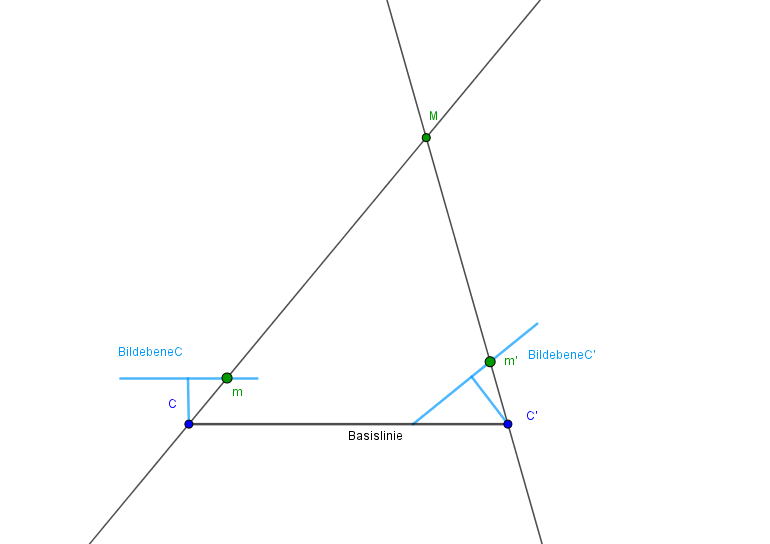
\includegraphics[width=\linewidth]{images/P_Solution_one.png}
%	\caption[Bestimmung extrinsischer Kameraparameter erste Lösung]{a)}
%	\label{fig:T_1}
	\endminipage\hfill
	\minipage{0.52\textwidth}
	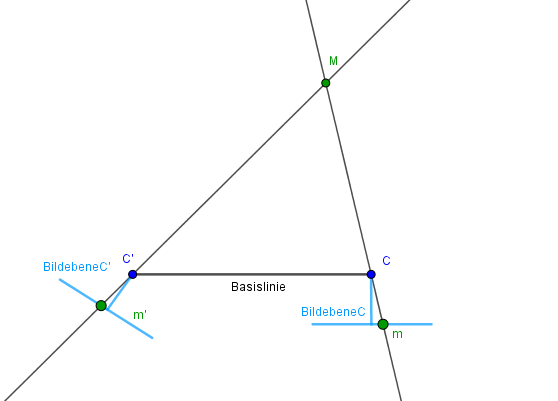
\includegraphics[width=\linewidth]{images/P_Solution_two.png}
	%\caption[Bestimmung extrinsischer Kameraparameter zweite Lösung]{b)}
%	\label{fig:T_2}	
	\endminipage\hfill	
	\caption[Bestimmung extrinsischer Kameraparameter Lösung eins und zwei]{In den ersten beiden Abbildungen kommt es zu einer Umkehrung der Basisline.}
	\label{fig:T_1}
\end{figure}
\begin{figure}[!htb]
	\minipage{0.52\textwidth}
	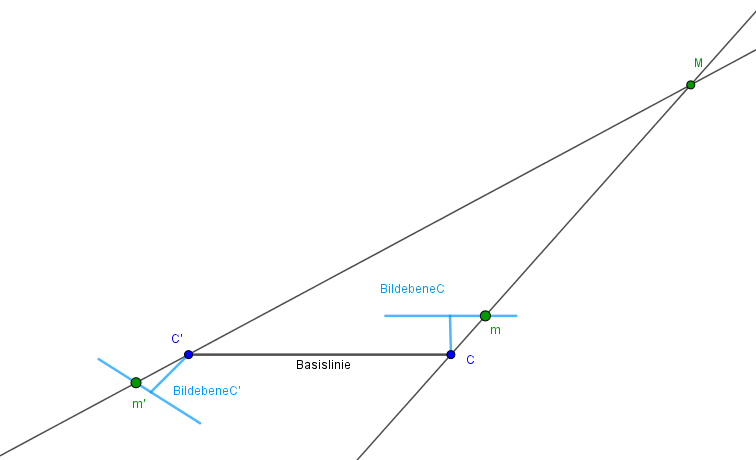
\includegraphics[width=\linewidth]{images/P_Solution_three.png}
%	\caption[Bestimmung extrinsischer Kameraparameter dritte Lösung]{c)}
%	\label{fig:T_3}
	\endminipage\hfill
	\minipage{0.5\textwidth}
	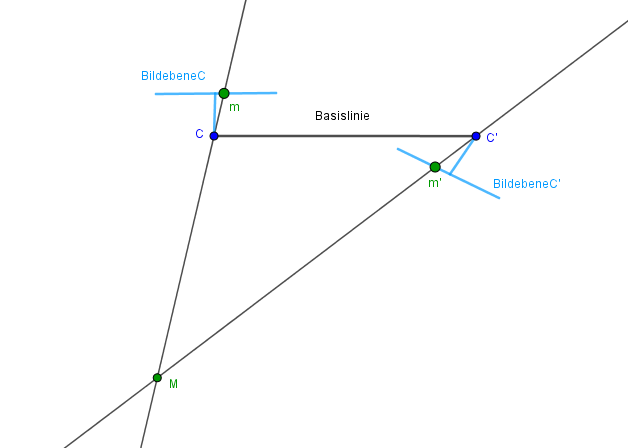
\includegraphics[width=\linewidth]{images/P_Solution_four.png}
	%\caption[Bestimmung extrinsischer Kameraparameter vierte Lösung]{d)}
%	\label{fig:T_4}
	\endminipage\hfill
	\caption[Bestimmung extrinsischer Kameraparameter Lösung eins und zwei]{In den beiden Abbildungen wird $C'$ und $180^\circ$ gedreht}
	\label{fig:T_2}
%	\caption[Alle vier Lösungen im Überblick]{Die Abbildungen a, b, c und d veranschaulichen, welche Bilder aus den vier Lösungen entstehen. In den Abbildungen a und b kommt es zu einer Umkehrung der Basisline. In den Abbildungen c und d wird $C'$ und $180^\circ$ gedreht}
\end{figure}
\pagebreak

%Zur Bestimmung der Abbildungsvorschrift wird die Fundamentalmatrix $F$ aus den korrespondierenden Punkten bestimmt. Die korrespondierenden Punkte sind Bildpunkte auf den verschiedenen Bildebenen eines gleichen Ursprungspunktes. Anhand des in Kapitel \ref{sec:HFE} beschriebenen 8-Punkte-Algorithmus, wird $F$ bestimmt. Über $F$ wird die essentielle Matrix $E$, mit den aus Kapitel \ref{sec:HFE} ermittelt Bedingung aus Gleichung \ref{eq:Ep7}, bestimmt.\\
%
%In dieser Arbeit wird angenommen, dass die Kameras zuvor einzeln Kalibriert wurden und die intrinsischen Kameraparameter bereits bekannt sind. Für die Bestimmung der extrinsischen Kameraparameter wird ein Ansatz verfolgt, in welchen die essentielle Matrix zum Einsatz kommt. Die essentielle Matrix ist eine Spezialform der Fundamentalmatrix und beschreibt den \textit{Epipolar-Constraint}, vlg \ref{eq:Ep7}, zwischen den normierten Bildebenenkoordinaten\cite{HZ,Elements,ZZGXr,Zhang2014,Ferid}. 
%
%\begin{gather}
%\hat{m}'^T_{\tau'}.E.\hat{m}_\tau = 0 
%\end{gather}
%
%Sind $F$ und Kameramatrizen $K$ und $K'$ bekannt, kann die essentielle Matrix wie in Kapitel \ref{eq:Ep7} gezeigt aus $F$ bestimmt werden. Die essentielle Matrix ist eine Fundamentalmatrix, welche zu einem paar normierter Projektionsmatrizen $\hat{P}$ mit $\hat{P} = [I|0]$ und $\hat{P}'$ mit $\hat{P}'= [R'|V']$ korrespondierend ist\cite{HZ,Zhang2014,ZZGXr,Ferid}. Um die Projektionsmatrix $P'=K'[R'|V']$ auf die normierte Form zu bringen, müssen die intrinsischen Parameter für $K'$ bekannt sein\cite{HZ}. 
%
%\begin{gather}
%	m'_{\tau} = P' \cdot M_\delta\\
%	m'_{\tau} = K'[R'|C'] \cdot M_\delta\;\; | \cdot K'^{-1}\\
%	\end{gather}
%	
%Die Inverse $K^{-1}$ wird auf beiden Seiten der Gleichung von links multipliziert\cite{HZ}.
%
%\begin{gather}
%	K'^{-1} \cdot m'_{\tau} = K'^{-1} \cdot K'[R'|C'] \cdot M_\delta\\
%	\hat{m}'_{\tau} = [R'|C'] M_\delta
%\end{gather}
%
%$M_\delta$ ist ein Objektpunkt im 3D-Raum, welcher mit $P'$ zum Bildebenenpunkt $m'_{\tau'}$ abgebildet wird. Nach der Normierung, wird $\hat{m}'_{\tau}$ als normierte Bildebenenkoordinate bezeichnet und die entstandene Projektionsmatrix $P' = [R'|C']$ als normierte Projektionsmatrix\cite{HZ,Ferid}. $E$ wird aus $F$ bestimmt mit:

%\begin{gather}
%E = K'^TFK
%\end{gather}

%det(E) = det(t×) det(R) = 0. Somit enth¨alt die Essentialmatrix
%nur zwei linear unabh¨angige Zeilen- oder Spaltenvektoren und hat den
%Rang4 Rg(E) = 2.
%Wie die Fundamentalmatrix muss auch die essentielle Matrix einen Rang von 2 haben. Des Weiteren darf eine 3 $\times$ 3-Matrix nur dann als essentielle Matrix bezeichnet werden, wenn die Singulärwerte, bestimmte Merkmale aufweisen. So müssen zwei der drei Singulärwerte gleich und die dritte null sein\cite{HZ}. Des Weiteren muss für die Determintante gelten, dass $det(E) = 0$ ist und die Quadratwurzel der Eigenwerte müssen wieder die Singulärwerte ergeben\cite{Ferid}. 

%\subsection{Bestimmung der extrinsischen Kameraparameter}

%(Noch einen Ansatz einbauen wie man die richtige Lösung algorithmisch auswertet? Im implementierte Algorithmus der arbeit wurden die Vier Lösungen jeweils rekonstruiert und alle ergebnisse ausgegeben.)

\subsection{Szenenrekonstruktion durch Triangulation}

Als Triangulierung wird in der Computer Vision die Bestimmung eines 3D-Objektpunktes aus korrespondierenden Bildpunkten bezeichnet. Als Voraussetzung für die Rekonstruktion müssen die jeweiligen korrespondierenden Bildpunkte und die Kameraparameter der einzelnen Kameras bekannt sein. Die Triangulierung funktioniert wie eine umgekehrte Projektion der Bildpunkte auf der Bildebene in einen Objektpunktes im Raum. Zwei Geraden, welche jeweils durch die Projektionszentren und den zu rekonstruierenden Bildpunkten gehen,  treffen sich im Raum. Der Schnittpunkt beider Geraden bildet den zu den Bildpunkten gehörenden Ursprungspunkt, wie in Abbildung \ref{fig:TriangulationOptimal} schematisch dargestellt ist.  \\\\


%wird das Rekonstruieren der Ursprünglichen 3D-Objektpunkte durch eine Rückprojektion vom jeweiligen Projektionszentrum der Kameras durch ihre Bildpunkte bezeichnet. Im synthetischen Beispiel wird durch einfache Schnittpunktberechnung derjenigen Geraden, welche durch die jeweiligen Projektionszentren und deren Bildpunkte auf deren Bildebenen gehen, der Ursprungspunkt im Raum rekonstruiert.\\


%\begin{minipage}{\linewidth}
%	\centering
%	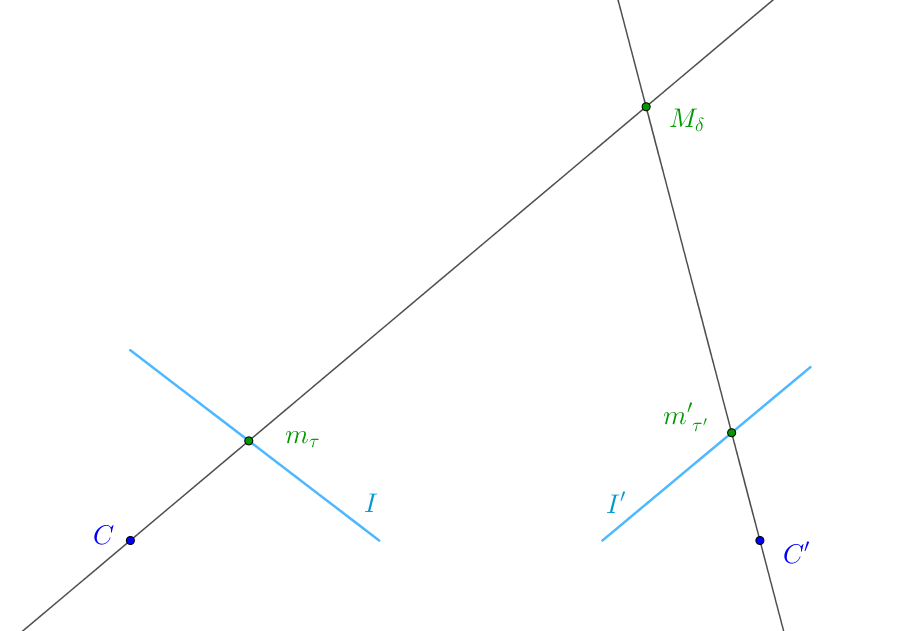
\includegraphics[width=0.8\linewidth]{images/optimaleTriangulierung.png}
%	\captionof{figure}{Optimale Triangulierung: Beide Geraden Treffen sich in einem Punkt im 3D-Raum} 
%	\label{fig:TriangulationOptimal}
%\end{minipage}\\ \\

\begin{figure}[!htb]
	\centering
	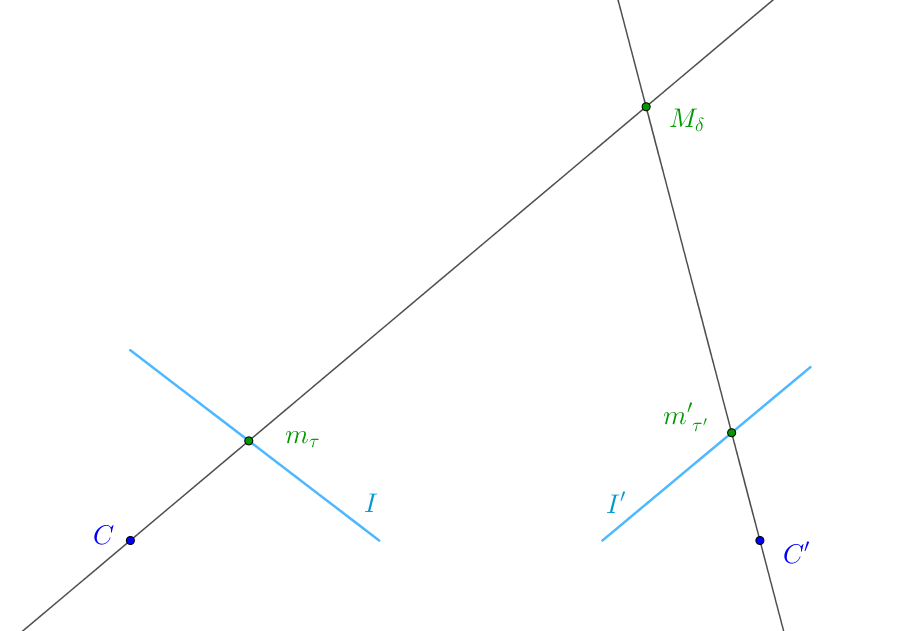
\includegraphics[width=0.8\linewidth]{images/optimaleTriangulierung.png}
	\caption[Einfache Triangulation]{Optimale Triangulierung: Beide Geraden Treffen sich in einem Punkt im 3D-Raum} 
	\label{fig:TriangulationOptimal}
\end{figure}

%bei der Szenenrekonstruktion realen Stereoaufnahmen kann eine Triangulation nicht so ohne weiteres durchgeführt werden. Bei einer Bildaufnahme mit Kameras, kommt es nicht selten vor, dass 
%
%In Realbildern, können Bildfehler wie beispielsweise Rauschen nicht vermieden werden, des Weiteren können korrespondierende Punkte nicht immer exakt auf den Pixel genau bestimmt werden.
% 
%Anders hingegen wäre es in einem realen Beispiel mit korrespondierenden Punkten, welche Beispielsweise über einen \textit{SURF}- Algorithmus detektiert wurden\cite{Mandun}. Diese Fehler führen dazu, dass wenn ein Schnittpunkt der Geraden durch die vermeintlichen korresponiderenden Punkte nicht gefunden werden kann, da die Geraden sich sehr wahrscheinlich nicht in einem Punkt treffen werden\cite{Mandun,HZ}. 
%
%
%\begin{minipage}{\linewidth}
%	\centering
%	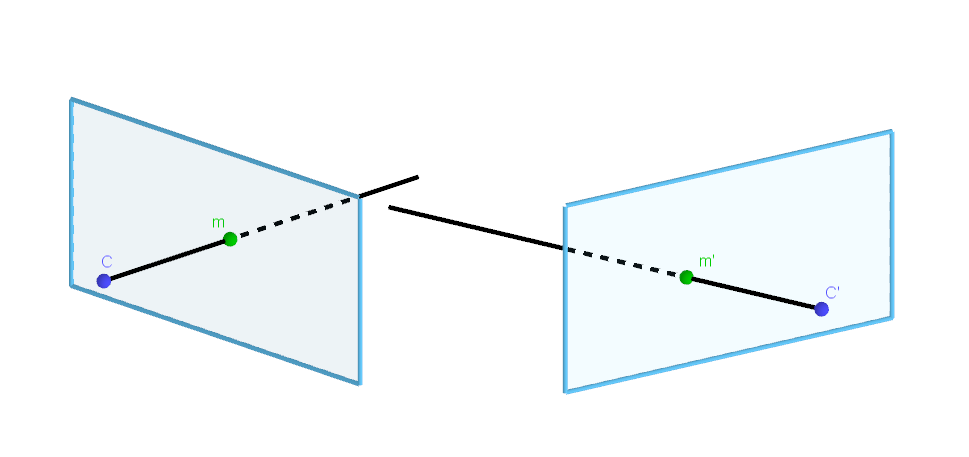
\includegraphics[width=0.8\linewidth]{images/problemTriangulation.png}
%	\captionof{figure}{Durch Ungenauigkeiten in der korrespondierenden Punkte, verfehlen sich die Linien und es kommt zu keinem Schnittpunkt} 
%\end{minipage}\\ 
%
%Für diese Fälle gibt es mehrere Näherungsverfahren, wovon eines, im Kapitel \nameref{sec:sampson}, im Realbeispiel eingeführt wird\cite{HZ}. In diesem Minimalbeispiel tritt der optimale Fall ein. Das bedeutet, dass ein zu Bildpunkt $m$ korrespondierender Bildpunkt $m'$ auf der zu $m$ korrespondierenden Epipolarlinie $l'$ liegt und somit garantiert ist, dass sich die Geraden $\overline{mM}$ und $\overline{m'M}$ auf jedenfall in einem gemeinsamen Punkt schneiden.
%
% Um den Schnittpunkt beider Geraden zu berechnen, werden zum einen die Bildpunkte  $A_\tau,B_\tau,C_\tau,D_\tau,A2_\tau,B2_\tau,C2_\tau,D2_\tau$ und $A_{\tau'},B_{\tau'},C_{\tau'},D_{\tau'},A2_{\tau'},B2_{\tau'},C2_{\tau'},D2_{\tau'}$, sowie die korrekt ermittelte Projektionsmatrix $P'$ von zuvor benötigt. 

Im synthetischen Beispiel wird mit reinen Daten gearbeitet. Das heißt, die Bildpunkte wurden mathematisch von ihrem Ursprungspunkt im Raum berechnet und sind somit frei von Verfälschungen durch äußere Einflüsse. Ein zum Bildpunkt $m_\tau$ korrespondierender Bildpunkt $m'_{\tau'}$ liegt genau auf der zu $m_\tau$ korrespondierenden Epipolarlinien $l'$. Somit ist garantiert, dass sich die Bildpunkte $m_\tau$ und $m'_{\tau'}$ bei einer Rückprojektion in einem Punkt $M_{0,\delta}$ im Raum treffen. Durch die zuvor erwähnte Skaleninvarianz der extrinsischen Kameraparameter handelt es sich bei $M_{0,\delta}$ jedoch noch nicht um den eigentlichen Ursprungspunkt $M_\delta$. \\

%Um die Rekonstruktion im synthetischen Beispiel so nah wie möglich an einem realen Beispiel zu halten, wird davon ausgegangen, dass nur die Kameraparameter und die jeweiligen Bildkoordinaten bekannt sind.\\


Vor der Bestimmung der extrinsischen Kameraparameter wurde festgesetzt, dass $T = [I|-0]$ die Translationsmatrix von $C$ ist. Somit gilt für die Projektionsmatrix von $C$, dass $P= K_0T =K_0[I|-0]$ ist. Die Projektionsmatrix $P'$ für $C'$ setzt sich aus einer der Lösungen von $T'$ und der Kameramatrix $K_0'$ zusammen, sodass gilt $P'=K_0'T' = K[R'|-RC]$.\\

Um eine Gerade von den Projektionszentren $C$ und $C'$ durch die jeweiligen Bildpunkte bilden zu können, müssen die Positionen von $C$ und $C'$ bekannt sein. Da die Koordinatensysteme $(C,\beta)$ und $(O,\delta)$ deckungsgleich sind, und $P = K_0[I|-0]$ ist, gilt $C = (0,0,0)^T$.  Um $C'$ aus $T' = R'[R'|-R'C']$ zu bestimmen wird der Translationsvektor $-R'C'$ aus $T'$ mit dem transponierten Rotationsmatrix $R'^T$ aus $T'$ multipliziert.

\begin{gather}
	C' =  R'^T \cdot -R'C' 
\end{gather}

%Nachdem die Position der Kamerazentren $C$ und $C'$ bekannt sind werden die Bildpunkte noch in Koordinaten bezüglich der jeweiligen Kamerakoordinatensysteme $(C,\beta)$ und $(C',\beta')$ transformiert. Dazu werden die zweidimensionalen Bildpunkte $m_\tau$ und $m_\tau'$ um den jeweiligen Abstand des Projektionszentrums zur Bildebene, sprich $\zeta$ und $\zeta'$, erweitert.
%

Die zweidimensionalen Bildpunkte werden mit den bekannten Brennweiten $\zeta$ und $\zeta'$ aus $K_0$ und $K_0'$ zu einer dreidimensionalen Koordinate erweitert.

\begin{gather}
	\begin{pmatrix}
	m_{\tau x}\\
	m_{\tau y}\\
	\end{pmatrix} \leadsto 
		\begin{pmatrix}
	m_{\tau x} \\
	m_{\tau y}\\
	\zeta
	\end{pmatrix}\\
		\begin{pmatrix}
	m'_{\tau' x}\\
	m'_{\tau' y}\\
	\end{pmatrix} \leadsto 
	\begin{pmatrix}
	m'_{\tau' x} \\
	m'_{\tau' y}\\
	\zeta
	\end{pmatrix}	
\end{gather}

Danach werden für die Rückprojektion zwei Geradengleichungen aufgestellt. Eine Gerade geht durch $C$ und $	\begin{pmatrix}
m_{\tau x} \\
m_{\tau y}\\
\zeta
\end{pmatrix} $ die zweite Gerade geht durch die Punkte $C'$ und $	\begin{pmatrix}
m'_{\tau' x} \\
m'_{\tau' y}\\
\zeta'
\end{pmatrix}$. Anschließend wird aus den zwei Geraden der Schnittpunkt $M_{\delta,0}$ im Raum bestimmt. $C$ und $C'$ sind aus Sicht des Weltkoordinatesystems $(O,\delta)$ definiert. $m'_{\tau'}$ wird in Koordinaten bezüglich des Kamerakoordinatesystem $(C,\beta)$ transformiert mit $m'_\beta = \begin{bmatrix}
R[I|-C']
\end{bmatrix}^{-1} \cdot m'_{\tau'}$.



\begin{gather}
	 g:= \vec{C} + t \cdot 
	\begin{pmatrix}
	 	\vec{C} -	
	\begin{pmatrix}	
	m_{\beta x} \\
	m_{\beta y}\\
	\zeta
	\end{pmatrix}
 \end{pmatrix} \\
g' := \vec{C'} + t \cdot 
\begin{pmatrix}
	\vec{C'} -
	\begin{pmatrix}
	m'_{\beta x} \\
	m'_{\beta y}\\
	\zeta'
	\end{pmatrix}
\end{pmatrix}
\end{gather}


 
%
%Nun muss für jedes Linienpaar eine Lösung für $t$ und $t'$ gefunden werden und die Lösungen in die Gleichungen 4.65 und 4.66 eingesetzt werden. Es sollte für beide Gleichungen die selbe Lösung für den rekonstruierten Punkt $A$ im Raum ergeben. Die Lösung entspricht meist noch nicht exakt dem eigentlichen Ergebnis, das liegt an der zuvor erwähnten Skaleninvariants der Rekonstruktion der exterenen Kameraparameter. 

Bei den zuvor ermittelten extrinsischen Kameraparametern ist der Translationsvektor skaleninvariant. Dies führt dazu, dass der rekonstruierte Objektpunkt $M_{\delta,0}$ nach der Szenenrekonstruktion noch nicht dem Ursprünglichen $M_\delta$ entsprechen muss. Dementsprechend wird als letzter Schritt die rekonstruierte Szenen anhand einer bekannten Referenzgröße skaliert. Als Referenzgröße kann beispielsweise ein zuvor abgemessener Abstand zwischen zwei Punkten in der Szene dienen. Im synthetischen Aufbau sind beispielsweise die Abstände zwischen den Originalbildpunkten bekannt. Die Abbildung \ref{fig:scale3} zeigt die Szene des Quaders mit unterschiedlichen Skalierungen. Die Abbildung \ref{fig:Quader1} zeigt die rekonstruierte Szene des synthetischen Beispiels auf uhre Ursprungsgröße skaliert.

%ihrer Originalgröße entsprechen. 
%
%Es wird noch ein Skalierungsfaktor benötigt, welcher die Szene auf Originalgröße skaliert. Hierfür ist es in einer Realszene ratsam, wenn man zuvor von zwei Punkten in Szene den Abstand zueinander abmisst, um anhand dessen einen Skalierungsfaktor zu berechnen. Im hier beschriebenen Minimalbeispiel sind die Originalkoordinaten der Objektpunkte im Raum bekannt, weshalb hier nach dem passenden Vielfachen der Rekonstruierten Punkte gesucht werden kann.
%
% Da die Verhätnisse der Abstände der Punkte zueinander bei der skalierung beibehalten wird, kommt zu keinen Verfälschungen des Objektes, da die Rotationen der beiden Kameras unangetastet bleibt. 


\begin{figure}[!htb]
	\minipage{0.40\textwidth}
	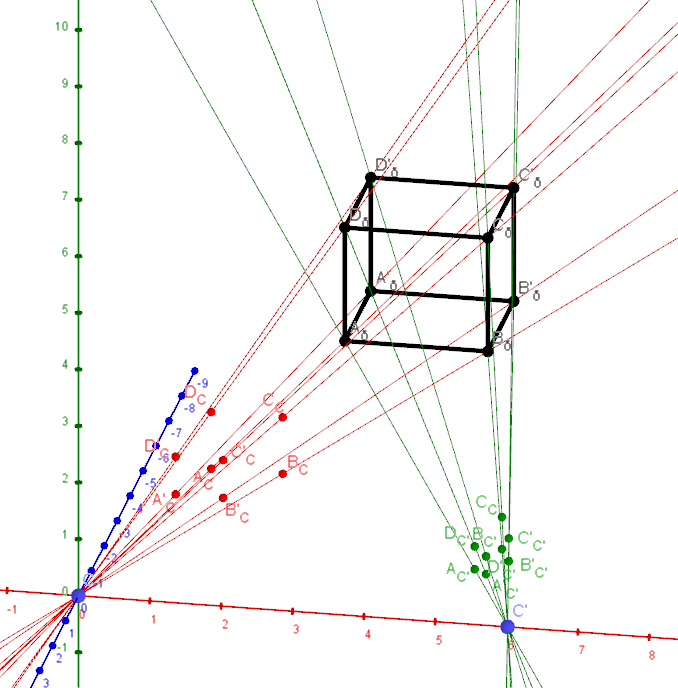
\includegraphics[width=\linewidth]{images/ScaleInvariance_1.png}
%	\caption{}
%	\label{fig:scale1}
	\endminipage\hfill
	\minipage{0.40\textwidth}
	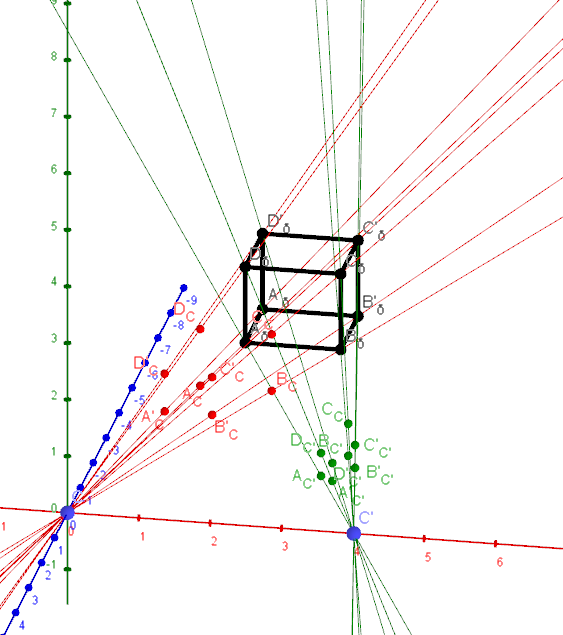
\includegraphics[width=\linewidth]{images/ScaleInvariance_2.png}
%	\caption{}
%	\label{fig:scale2}
	\endminipage\hfill
\end{figure}

\begin{figure}[!htb]
	\centering
	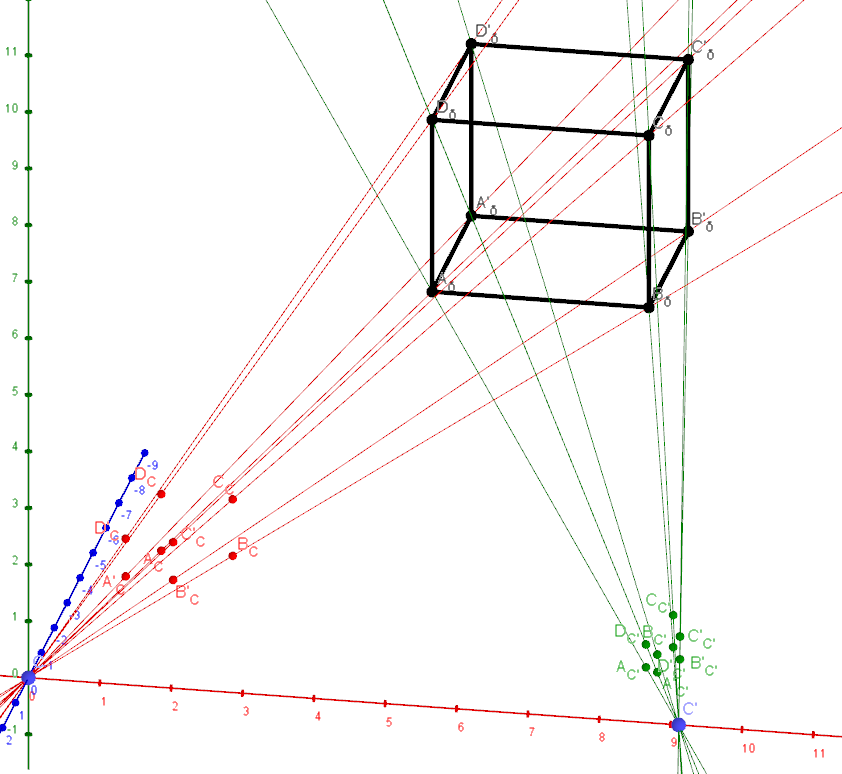
\includegraphics[width=0.40\linewidth]{images/ScaleInvariance_3.png}
	\caption[Skalierung der Rekonstruierten Szene]{Veranschaulichung der Skaleninvarianz und dessen Auswirkung auf die geometrische Form und Größe der Objekte} 
	\label{fig:scale3}
\end{figure}
\pagebreak



\begin{figure}[!htb]
	\minipage{0.42\textwidth}
	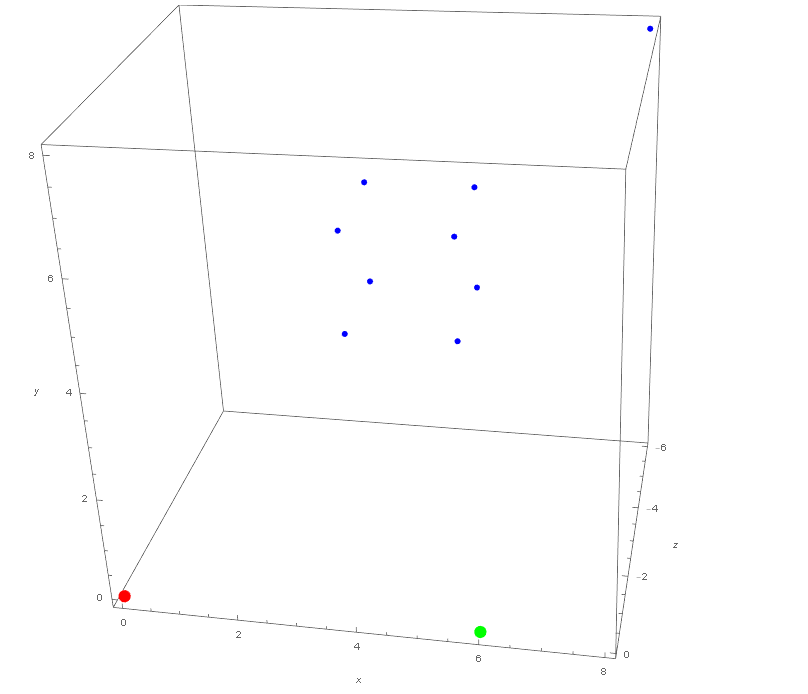
\includegraphics[width=\linewidth]{images/MinimalBeispiel_reconstructed.png}
	%\caption{}
	\endminipage\hfill
	\minipage{0.42\textwidth}
	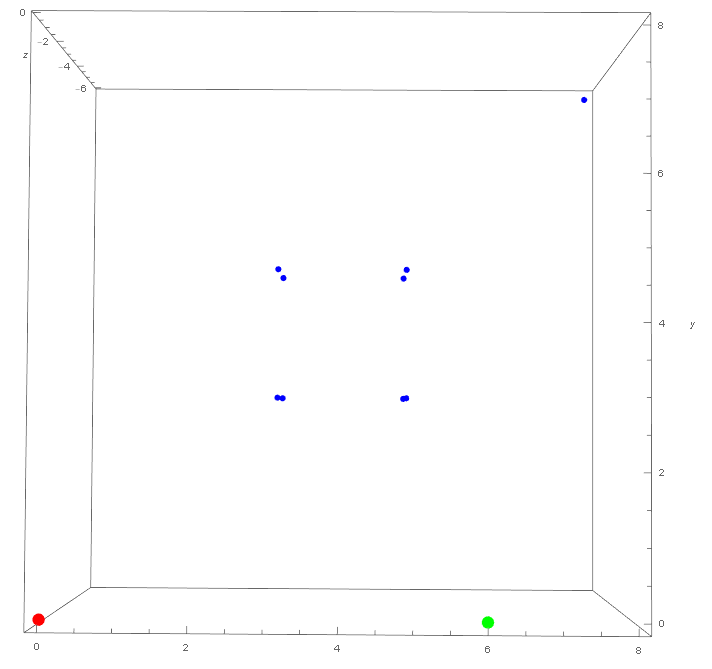
\includegraphics[width=\linewidth]{images/MinimalBeispiel_reconstructed_3.png}
%	\caption{}
	\endminipage\hfill
	\caption[Programmplot der rekonstruierten Szene]{Der rote Punkt stellt die Postion von $C$ dar, der grüne steht für die Position von $C'$ relativ zu $C$. Die blauen Punkte stellen den rekonstruierten Quader und den extern platzierten neunten Punkt da. Die Abbildungen entstand aus dem in \textit{Mathematica}\cite{Mathematica} implementierten Algorithmus.}
		\label{fig:Quader1}
\end{figure}
\pagebreak



		
		%------------------------------------------------------------%
			%% Kapitel 2 / Chapter 2 (C2)
		%------------------------------------------------------------%
		
		% C2 - example 1
		\chapter{Auswirkungen von unterschiedlichen Kameraauflösungen}
\label{sec:minimalAuf} 

Wenn man sich mit digitalen Bilddaten auseinandersetzt, so kommt man nicht drum herum sich auch mit den  verschiedenen Auflösungsarten beschäftigen zu müssen. Im vorherigen Kapitel wurde gezeigt, wie eine 3D-Szene aus zwei heterogenen Bildquellen, welche von zwei Kameras gleicher Auflösung aufgenommen wurden, rekonstruiert werden konnte und gleichzeitig noch die externen Kameraparameter von $C'$ in Relation zu $C$ geschätzt werden konnten. Dies wirft die Frage auf, welche Auswirkungen Bilder zweier Kameras mit unterschiedlichen Auflösungen für die Rekonstruktionen haben können. Aus der Stereokalibrierungsapp, welche \textit{MatLab} anbietet, ist bekannt, dass diese nicht mit Bildern unterschiedlicher Auflösung eine Szenerekonstruktion durchführen kann. Der erste Schritt bestand erstmal darin zu überprüfen, warum zwei unterschiedliche Auflösungen in \textit{MatLab} Probleme machen. \textit{MatLab} verfolgt einen etwas anderen Rekonstruktionsansatz. Zu aller erst werden die Kameras kalibriert. Dies geschieht über die Matlab-Funktion \text{estimateCameraParameters}\cite{MatlabCamParam}. Diese Funktion funktioniert auch bei Bildern unterschiedlicher Auflösung noch ohne Probleme. Das Problem, welches sich als eigentlich minimales Problem herausstellt, ist, dass die darauf folgenden Rektifizierung der Stereobilder nicht mit zwei Bildern unterschiedlicher Auflösung funktioniert. In den \textit{MatLab} references, steht es nicht expliziet drin \cite{MatlabRec}. Die Rektifizierung in Matlab funktioniert nach einem Schema, welches ähnlich dem aufgezeigten Beispiel im Kapitel \nameref{sec:rectification} bereits erwähnt wurde und in \cite{Fusiello,FusielloSite} nochmal genau aufgeführt wird. Das Problem liegt also nicht daran, dass bilder unterschiedlicher Auflösung nicht rektifiziert werden können, sondern das Problem liegt an dem in \textit{MatLab} verwendeten Algorithmus für die Rektifizierung zweier Stereobilder (Foren Zitieren????). Warum \textit{MatLab} überhaupt rektifiziert, liegt daran, dass ein Ansatz der Szenerekonstruktion gewählt wurde, welcher die essentielle Matrix nicht benötigt. In diesem Falle, werden zwei Stereobilder aufgenommen, danach rektifiziert und anschließend über eine sogenannte \textit{Disparity-Map}, die Szenen punkte rekonstruiert\cite{MatlabDisp,MatlabStereoApp,Fusiello,Javier}. Der in dieser Arbeit gewählte Rektifizierungsalgorithmus, ist nicht auf gleiche Kameraauflösungen beschränkt. Mittlerweile gibt es natürlich deutlich fortgeschrittenere Rektifizierungsansätze, jedoch wurde für diese Arbeit der Ansatz von \cite{ZZ} gewählt, um ein Gefühl zu vermitteln, dass wenn man sich auf die Epipolargeometrie bezieht, die Auflösungen der Kameras keine Rolle spielen\cite{Elements}. Was genau unterschiedliche Auflösungen der Kameras für die einzelnen Bilder bedeutet und was genau sich bei der Aufnahme mit dem Sensor dabei ändert, soll im folgenden Unterkapitel kurz erläutert werden. Danach wird aufgezeigt, was genau diese Veränderungen für die Epipolargeometrie bedeuten und letztendlich wird das Minimalbeispiel so angepasst, als hätten zwei Kameras unterschiedlicher Auflösung die selbe Szene wie davor aufgenommen und die Resultate miteinander verglichen. 

\section{Abbildungsunterschiede}

%Hier vllt kurz erklären was unterschiedliche Auflösung für die Funktion eines Sensors bedeutet (Interpolierung mehrerer Pixel, Nicht nutzung des gesammten Pixelspektrums)\\
%
%
%Aufbau eines CCD Sensors und dessen funktionen\\
%
%Ein Bildsensor, der dieses Prinzip zum Verschieben und Auslesen der Ladungen der lichtaktiven Pixel anwendet, wird ''CCD-Sensor'' genannt.\\
%
%Allgemein werden einige typische CCD-Sensor-Bauarten unterschieden, die auf weiteren Homepage-Seiten beschrieben werden:
%
%\begin{itemize}
%	\item Interline Transfer CCD
%	\item Full Frame Transfer CCD
%	\item Frame Transfer CCD
%\end{itemize}
%
%von denen sich in der industriellen Bildverarbeitung vor allem der so genannte "Interline Transfer Sensor" durchgesetzt hat.
%
%\begin{itemize}
%	\item In der Masse der industriellen Applikationen werden Kameras mit CCD-Sensoren verwendet. Sie sind rauscharm, lichtempfindlich, haben eine hohe Uniformität und sind aufgrund Ihrer linearen Charakteristik geeignet für präzise Messapplikationen.
%	\item Eine überwältigende Mehrheit der Hersteller industrieller Kameras verbaut in Ihren Standardmodellen CCD-Sensoren, die in 90\% der Fälle von der Fa. Sony stammen. Über die Jahre hinweg wurden immer wieder neue, weiter entwickelte Sensoren auf den Markt gebracht. Überprüfen Sie, falls Sie besonders hohe Ansprüche an Ihren Sensor haben, ob eine neuere oder ältere Sensorvariante verwendet wird.
%	\item Aufgrund verbesserter Fertigungstechnologien werden höhere Empfindlichkeiten der Pixel erzielt, die damit (bei Beibehaltung der Qualität) immer kleinere Pixelgrößen erlauben. Die Anforderungen an die Qualität der Optik sind dadurch extrem gestiegen.
%	\item CCD-Sensoren mit besonders schnellen Frameraten oder mit besonders hoher Auflösung werden von der Fa. TrueSense (ehemals Kodak) entwickelt. Auch hier lohnt sich ein Blick auf das Datenblatt, welche Type (neue / alte Variante) verwendet wird.
%	\item Fast jeder Sensor hat eine gewisse Anzahl an Defektpixeln, die meistens aber kaum auffallen und manchmal von der Kamera-Firmware durch eine Pixel-Fehlerkorrektur heraus interpoliert werden können. CCD-Hersteller unterscheiden üblicherweise Ihre Sensoren in die Qualitätsstufen Grade "B", Grade "A" und Grade "zero", um die Anzahl der Defektpixel zu beschreiben. Diese unterscheiden sich preislich. Bei extrem kritischen Applikationen können  von bestimmten Kamera-Herstellern gegen Aufpreis auch Kameras mit Grade "zero"-Sensoren mit null Defektpixeln gekauft werden.
%	\item 
%	Etwa alle 6 Grad Temperaturerhöhung verdoppelt sich das thermische Rauschen der Pixel. Gute Kameras sollten im Betrieb nicht besonders warm werden. Vermeiden Sie außerdem die Montage der Kamera in Bereichen von Wärmestau.
%	
%\end{itemize}


Das Herz einer modernen Kamera ist der Halbleiter-Bildsensor. Die Bildsensoren spielen in der optischen Messtechnik und industriellen Bildverarbeitung eine große Rolle\cite{Photonik}. Die in dieser Arbeit verwendeten Kameras für die Aufnahme der Stereobildpaare, waren zum einen die Vollformatkamera Canon EOS 6D und die Halbformatikamera Canon EOS 60D. Beide besitzen einen CMOS-Sensorchip, welcher zu den Halbleiterbildsensoren gehört\cite{Canon6D}. Die Geometrie dieser Sensoren, ist grob gesprochen als eine $M \times N$ - Matrix, bestehend aus $M \times N$ Pixeln. Die Pixel bedecken nur einen Teil der Sensorfläche und können in ihrer geometrischen Beschaffenheit von der Form des Sensors unterschieden werden\cite{Photonik}. Abbildung 5.1 zeigt einen schematischen Aufbau eines Halbleiterbildsensors\\

\begin{minipage}{\linewidth}
	\centering
	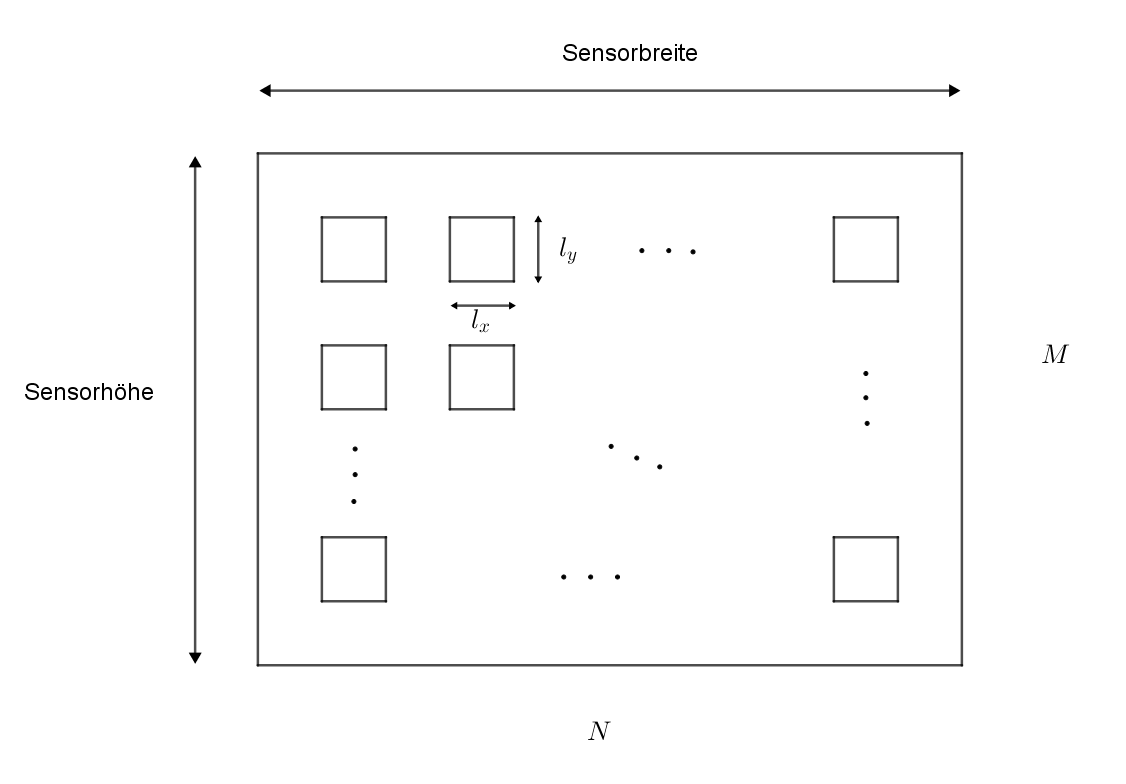
\includegraphics[width=.8\linewidth]{images/Bildsensor_mit_Pixel.png}
	\captionof{figure}{Rechteckiger Bildsensor mit darauf sich befindendenden quadratischen Pixeln. Vlg \cite{Photonik}} 
\end{minipage}\\ \\


Die Auflösung des Sensors hängt von den horizontalen und vertikalen Pixelabständen ab und gibt wieder, welche Objektdetails mit dem Sensor gerade noch erkannt werden können.\cite{Photonik}. Ein Sensor hat eine maximale Auflösung, welche durch die Anzahl seiner fest installierten Pixel bestimmt wird. Die Bildqualität ist abhängig von der Größe des Sensorchips und der Menge der sich darauf befindenden Pixel. Der CMOS-Sensor einer Canon 6D hat beispielsweise eine Größe von $36 \times 24 mm$ und eine maximale Auflösung von $5.472 \times 3.648$ Pixel. Jedoch ist das nicht die einzige Auflösung, welche beim fotographieren oder filmen mit der Kamera genutzt werden kann. Es können sowohl die Pixelanzahl als auch das Seitenverhältnis der entstehenden Bilder eingestellt werden. Bei der Canon EOS 6D können insgesamt vier verschiedene Seinsverhältnisse eingestellt werden $[3:2], \,[4:3], \,[16:9]$ und $[1:1]$\cite{Canon6D}. Die Bildauflösungen unterscheiden sich pro Seitenverhältnis in sechs Auflösungseinstellungen \textit{L, M, S1, S2, S3}. 

	\begin{table}[h]
	\centering
	\caption{Auflösungen Canon EOS 6D}
	\label{my-label}
	\begin{tabular}{c|c|c|c|c}
		\hline
		\rowcolor{blue!25} 	& 3:2 & 4:3 & 16:9 & 1:1 \\\hline		
		L	&  5478 $\times$ 3648 px & 4864 $\times$ 3648 px & 5472 $\times$ 3072 px & 3648 $\times$ 3648 px \\\hline		
		M &  4104 $\times$ 2736 px & 3648 $\times$ 2736 px & 4104 $\times$ 2310 px & 2736 $\times$ 2736 px \\\hline
		S1 &  2736 $\times$ 1824 px & 2432 $\times$ 1824 px & 2736 $\times$ 1536 px & 1824 $\times$ 1824 px \\\hline
		S2&  1920 $\times$ 1280 px & 1696 $\times$ 1280 px & 1920 $\times$ 1080 px & 1280 $\times$ 1280 px \\\hline
		S3&  720 $\times$ 480 px & 640 $\times$ 480 px & 720 $\times$ 408 px & 480 $\times$ 480 px \\\hline
	\end{tabular}
\caption{Vgl \cite{Canon6D}}
\end{table}

Je geringer die Auflösung, desto geringer ist die Anzahl der Pixel. Die Anzahl der Pixel auf einem Sensorchip kann natürlich nicht variieren. Eine geringere Pixelanzahl bei gleichbleibender Bildgröße, bedeutet, dass sich ein Pixel mit den um sich befindedenden Pixeln interpoliert, so dass ein neuer Pixel bestehend aus mehreren kleinen Pixeln entsteht. Dieser Prozess wird Nachbarschaftsoperation genannt. Für die Berechnung des neuen Bildpixels $px'$ an der Stelle $(m,n)$ wird nicht nur das Bildpixel $p$ des Originalbildes an der Stelle (m,n) verwendet, sondern auch einige seiner Nachbarpunkte\cite{Photonik}. Bei der Canon 6D bietet das Seitenverhältnis $[3:2]$ die Möglichkeit die maximale Pixelanzahl des Sensors zu verwenden, vergleiche hierzu Tabelle 5.1. Bei einem Seitenverhältnis von $[4:3]$ ist die Anzahl der maximal möglichen Pixel nur noch 4864 $\times$ 3648. Änders sich das Seitenverhätnis des Bildauschnitts, so wird auch nicht mehr die gesamte Fläche des Sensors benutzt. 

\begin{minipage}{\linewidth}
	\centering
	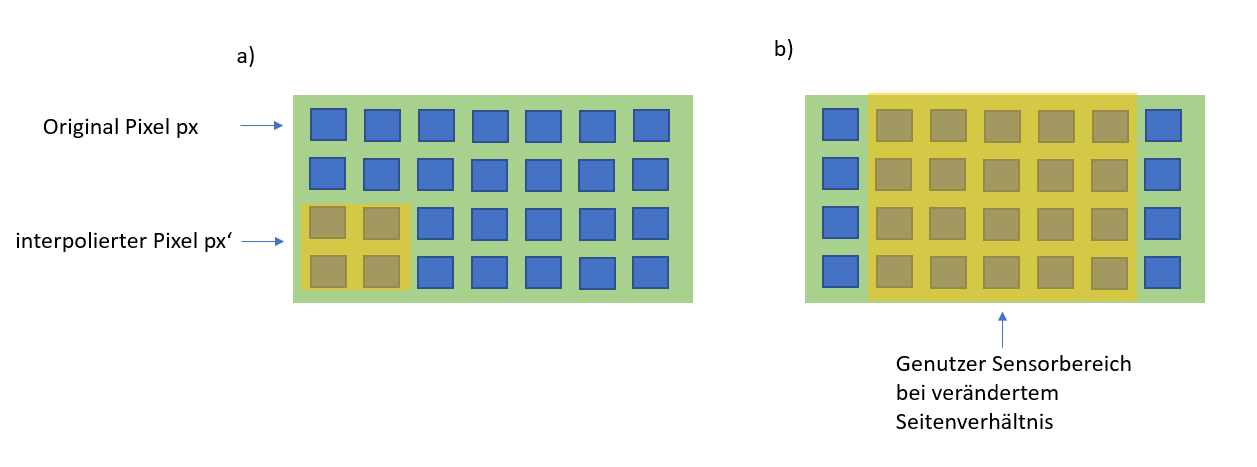
\includegraphics[width=1.\linewidth]{images/AufloesungSensor.png}
	\captionof{figure}{Bild a) zeigt die Interpolation von Pixeln, wenn bei gleichbleibenden Seitenverältnissten weniger Pixel für das Bild verwendet werden sollen. Die interpolierten Pixel leiten dann alle das selbe Signal weiter. Bild b) zeigt in gelb markiert, den verweneten Bereich des Sensors, wenn sich die Seitenverältnisse ändern und nicht mehr der volle Sensor genutzt wird.} 
\end{minipage}\\ \\

\section{Auswirkungen auf die Epipolargeometrie}

Um nun auf die Fragestellung der Auswirkung unterschiedlicher Auflösungen auf die Szenenrekonstruktion zu kommen, kann nun folgende behauptung aufgestellt werden. Beide Kameras besitzen einen Bildsensor, welcher fest in der Kamera installiert ist und sich weder in Position noch seiner Form ändern kann. Dieser Bildsensor beinhaltet sowohl das Bildebenenkoordinatensystem, bei welchem der Hauptpunkt den Koordinatenursprung bildet als auch das Sensorkoordinatensystem, dess Ursprung leicht außerhalb einer der Ecken des Sensors sich befindet. Abbildung ??? zeigt einen Stereoskopischen Szenenaufbau mit Kameras gleicher Auflösung. Die Sensorkoordinatensysteme besitzen die selbe Skalierung. 
\pagebreak
\begin{figure}[!htb]
	\minipage{0.52\textwidth}
	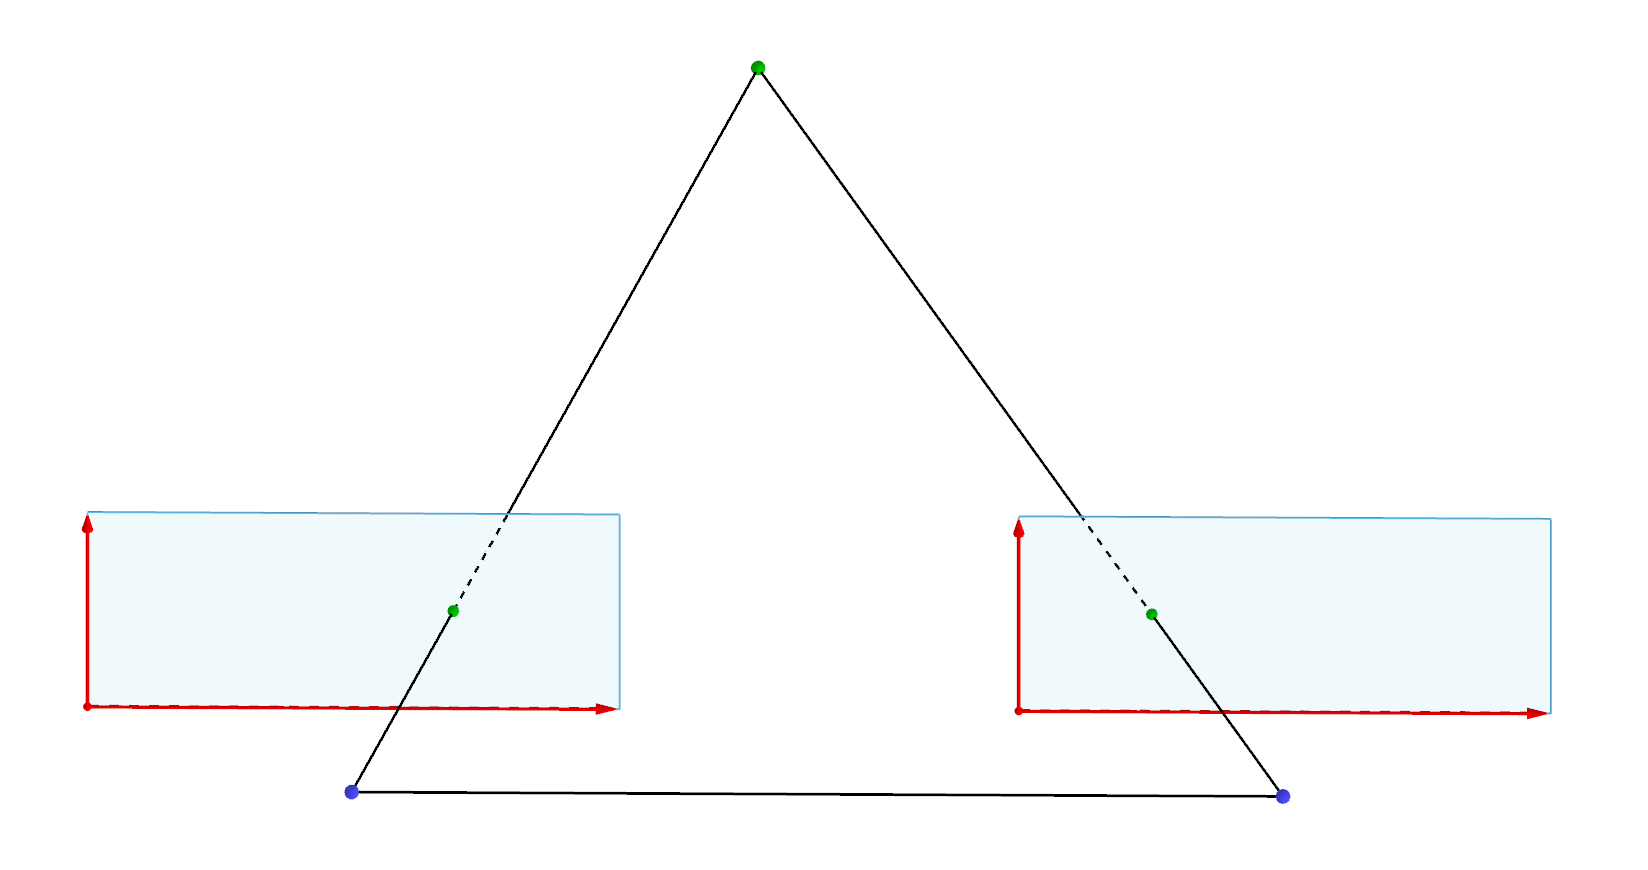
\includegraphics[width=\linewidth]{images/SensorSelbeAufloesung.png}
	\caption{$C$ und $C'$ haben die selbe Auflösung eingestellt}
	\label{fig:awesome_image1}
	\endminipage\hfill
	\minipage{0.52\textwidth}
	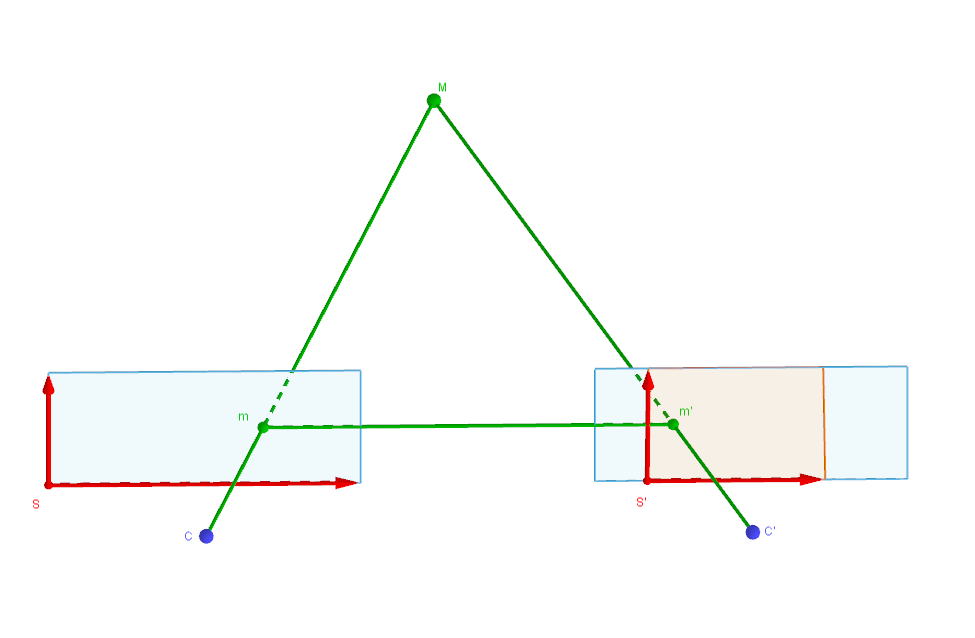
\includegraphics[width=\linewidth]{images/SensorUnterschiedlicheAufloesung.png}
	\caption{$C$ und $C'$ haben unterschiedliche Auflösungen eingestellt}
	\label{fig:awesome_image2}
	\endminipage\hfill
\end{figure}


Es bildet sich wieder das bekannte Dreieck zwischen den Bildpunkten $m_\sigma$ und $m'_{\sigma}$ und dem Objektpunkt $M_\delta$. Das in diesem Falle einen korrekte Szenenrekonstruktion funktioniert, ist im Kapitel \nameref{sec:minimal} anhand des Minimalbeispiels aufgezeigt worden. Wird die Auflösung auf einer der beiden Kameras verringert und damit einhergehend auch noch das Seitenverhältnis geändert, so ändert sich zum einen der aktive Teilbereich des Sensorschips, sowie die Skalierung der Werte auf den Koordinatenachsen des Sensorkoordinatensystems. Die Skalierung der Koordinatenachsen hängt mit der interpolation der mehrerer Pixel zu einem neuen Pixel zusammen. Abbildung 5.3 zeigt schematisch, was sich nach veränderten Auflösungseinstellungen am Sensor verändert.%(GRAFIK EINFÜGEN(hab vergessen welche!))\\
Epipolargeometrisch ändert sich wie man in Abbildung ??? sehen kann nichts. Das zuvor erwähnte Dreieck zwischen den Bildpunkten und dem Objektpunkt bleibt unverändert. Wie in Kapitel \nameref{sec:epipolar} bereits erwähnt, dürfen die Bildebenkoordinatensysteme und somit auch die Sensorkoordinatensysteme unterschiedlich voneinander sein\cite{Elements}. Für die relative Position des Bildpunktes auf dem Sensor ändert sich nichts, dieser bleibt statisch, einzig seine Koordinatenwerte ändern sich im bezug auf das Sensorkoordinatensystems. Für die Fundamentalmatrix und die Essentielle Matrix ergeben sich lediglich andere Vielfache voneinander, welches wie erwähnt ebenfalls gültige Lösungen sind \cite{HZ,Ferid}.

\section{Minimalbeispiel mit unterschiedlichen Kameraauflösungen}

Als Beweise der aufgestellten Behauptung wurde im Minimalbeispiel die Kameramatrix einer der Beiden Kameras unterschiedlich modifiziert. Während für die Kameramatrix von $C$ der Wert $\zeta = -1$ in der Kamermatrix $K$ bleib, wurde das $\zeta$ in $C'$ verändert, so dass sie drei verschiedene neue Kameramatrizen $K'_1, K'_2$ und $K'_3$ ergeben. Die resultierenden Abbildungen des Quaders sind in den Abbildungen ??? bis ??? zu sehen.



\begin{gather}
K = \begin{bmatrix}
-1&0&0&0\\
0&-1&0&0\\
0&0&-1&0\\
%0&0&1&0
\end{bmatrix}\\
K'_1 = \begin{bmatrix}
-2&0&0&0\\
0&-2&0&0\\
0&0&-1&0\\
%0&0&1&0
\end{bmatrix}\\
\end{gather}

\begin{gather}
K'_2 = \begin{bmatrix}
-3.2&0&0&0\\
0&-1.2&0&0\\
0&0&-1&0\\
%0&0&1&0
\end{bmatrix}\\
K'_3 = \begin{bmatrix}
-0.5&0&0&0\\
0&-4.3&0&0\\
0&0&-1&0\\
%0&0&1&0
\end{bmatrix}
\end{gather}\\


\begin{figure}[!htb]
	\minipage{0.48\textwidth}
	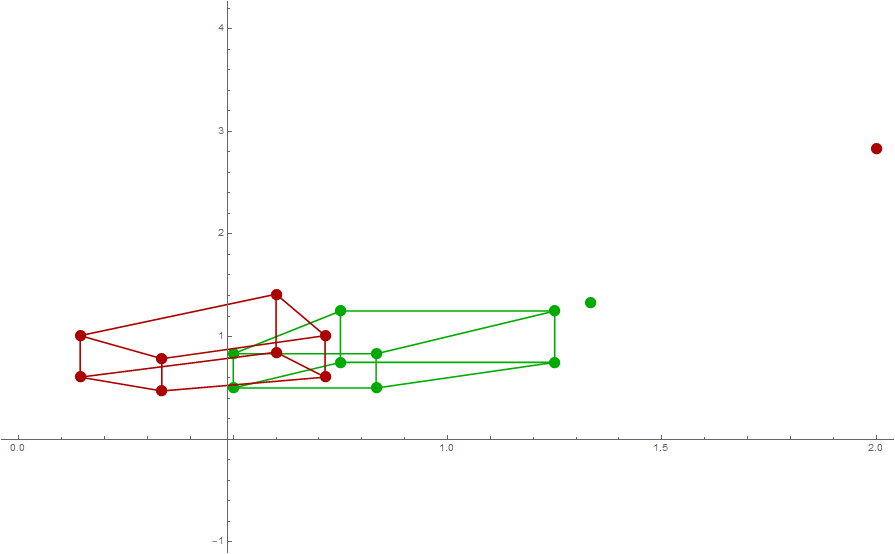
\includegraphics[width=\linewidth]{images/Zeta1.png}
	\caption{$C$ und $C'$ haben die selbe Auflösung eingestellt}
	\label{fig:awesome_image1}
	\endminipage\hfill
	\minipage{0.48\textwidth}
	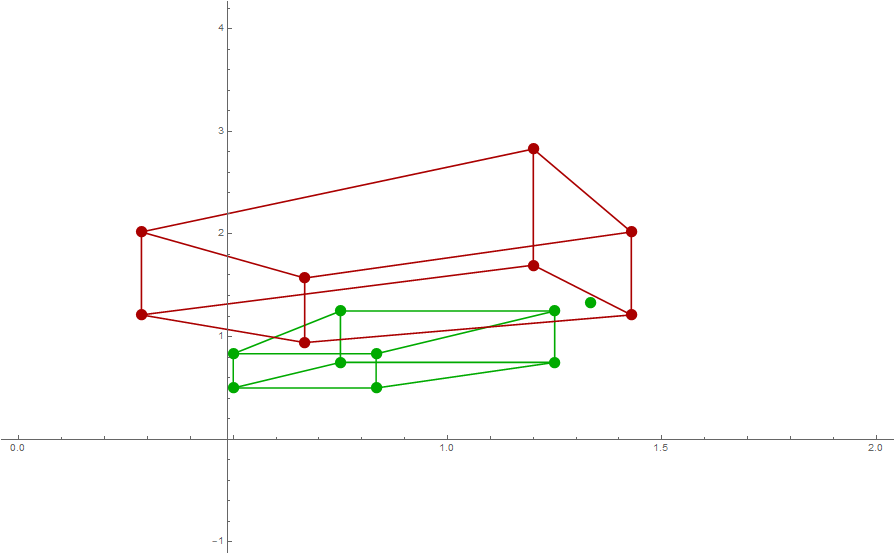
\includegraphics[width=\linewidth]{images/Zeta2.png}
	\caption{$C$ und $C'$ haben unterschiedliche Auflösungen eingestellt}
	\label{fig:awesome_image2}
	\endminipage\hfill
\end{figure}

\begin{figure}[!htb]
	\minipage{0.48\textwidth}
	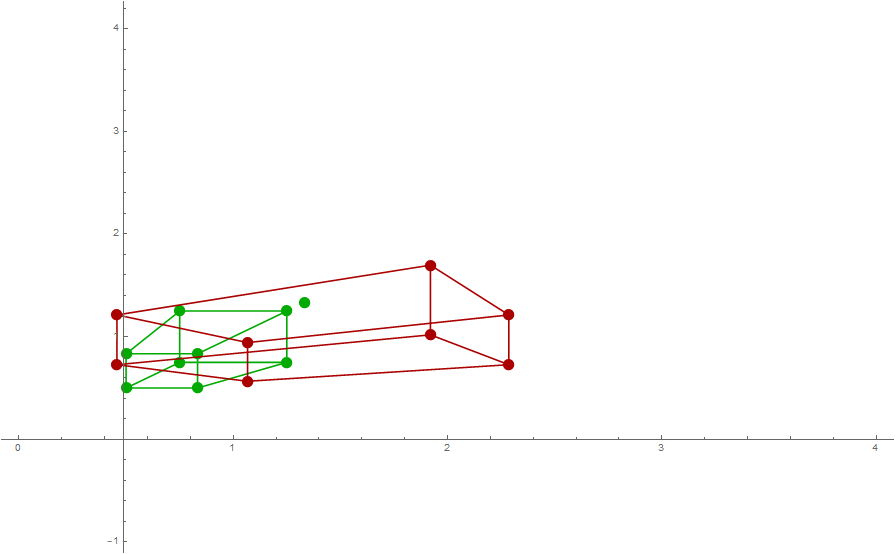
\includegraphics[width=\linewidth]{images/Zeta32_12.png}
	\caption{$C$ und $C'$ haben die selbe Auflösung eingestellt}
	\label{fig:awesome_image1}
	\endminipage\hfill
	\minipage{0.48\textwidth}
	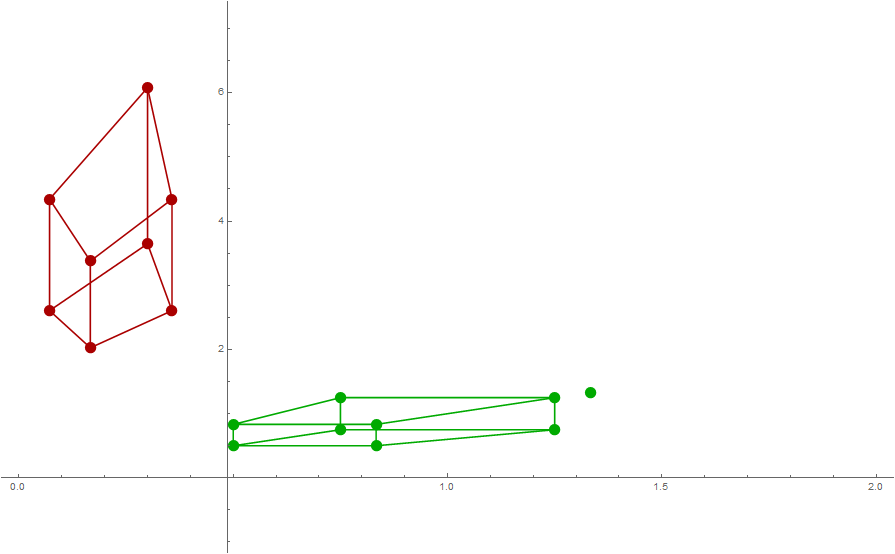
\includegraphics[width=\linewidth]{images/Zeta05_43.png}
	\caption{$C$ und $C'$ haben unterschiedliche Auflösungen eingestellt}
	\label{fig:awesome_image2}
	\endminipage\hfill
\end{figure}


%(GRAFIK $\zeta * 2, \zeta *3,2 und 1.2$, $\zeta * 0.5 und 4.3$ sagen dass das rote jeweils das mit dem verändertem $\zeta$ )\\


Während die Abbildung von $C$ Unverändert bleibt, wird in Abbildung??? Die Abbildung des Quaders in $C'$ ''vergrößert'', was für eine höhere Anzahl an verwendeten Pixeln steht. In Abbildung ??? werden die Pixel in horizontaler Richtung um das 3.2- fache und in vertikaler Richtung um das 1.2-fache erweitert und in Abbilung ??? wird in horzontaler Richtung die Anzahl der Pixel um das 0.5-fache und in vertikaler Richtung um das 4.3-fache skaliert. Für die Fundamentalmatrix und die essentielle Matrix ergeben sich verglichen mit denen aus dem Beipiel mit gleicher Abbildung folgende Matrizen.\\


\begin{gather*}
	\zeta_x = 1, \, \zeta_y = 1: \; \; \;\;
	F = \begin{pmatrix}
			0&-0.5&0\\
			0&0&\frac{1}{\sqrt{2}}\\
			0&-0.5&0
		\end{pmatrix} |: -0.5 \; \leadsto
	F=\begin{pmatrix}
		0&1&0\\
		0&0&-\sqrt{2}\\
		0&1&0
	\end{pmatrix}\\	
	\zeta_x = 2, \, \zeta_y = 2: \; \; \;
	F = \begin{pmatrix}
		0&0.378&0\\
		0&0&-0.534\\
		0&0.756&0
	\end{pmatrix} |: 0.756 \; \leadsto
	F=\begin{pmatrix}
		0&0.5&0\\
		0&0&-\frac{1}{\sqrt{2}}\\
		0&1&0
	\end{pmatrix}\\ \frac{1}{\zeta_x} = 0.5, \;\; \frac{\sqrt{2}}{\zeta_y} = \frac{1}{\sqrt{2}}\\
	\zeta_x = 3.2, \, \zeta_y = 1.2: \; \; \;
F = \begin{pmatrix}
	0&0.198&0\\
	0&0&-0.747\\
	0&0.634&0
\end{pmatrix} |: 0.634 \; \leadsto
F=\begin{pmatrix}
	0&0.312&0\\
	0&0&-1.178\\
	0&1&0
\end{pmatrix}\\ \frac{1}{\zeta_x} = 0.312, \;\; \frac{\sqrt{2}}{\zeta_y} = -1.178\\
	\zeta_x = 0.5, \, \zeta_y = 4.3: \; \; \;
F = \begin{pmatrix}
	0&0.885&0\\
	0&0&-0.145\\
	0&0.442&0
\end{pmatrix} |: 0.442 \; \leadsto
F=\begin{pmatrix}
	0&2&0\\
	0&0&-0.328\\
	0&1&0
\end{pmatrix}\\ \frac{1}{\zeta_x} =2, \;\; \frac{\sqrt{2}}{\zeta_y} = -0.328
\end{gather*}\\

%\begin{minipage}{\linewidth}
%	\centering
%	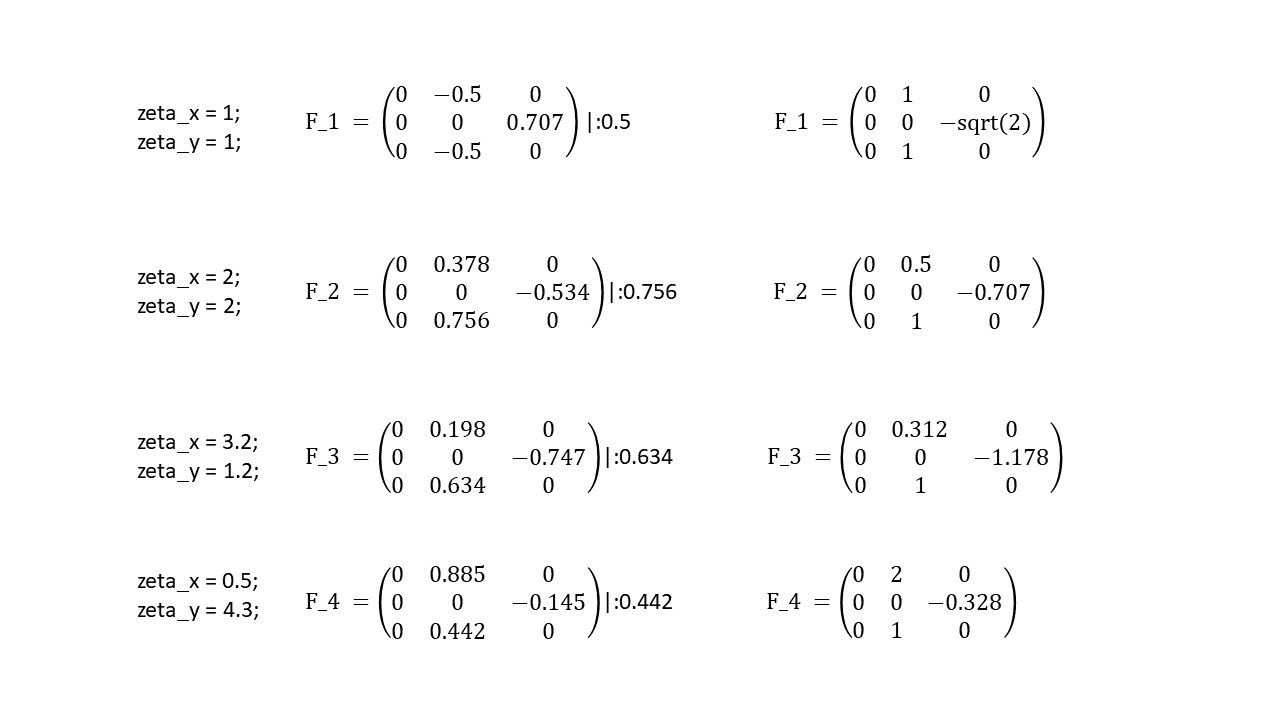
\includegraphics[width=1.\linewidth]{images/FundEMatrizen.png}
%	\captionof{figure}{Die Fundamentalmatrizen sind bei jeder Auflösung, die gewählt wurden immer Vielfache voneinander} 
%\end{minipage}\\ \\
(hier können vllt noch die verschiedenen rotationen gezeigt werden ,welche immer die selbe rotation bewirken)
Die Werte für $\zeta_x$ wirken sich auf die erste Zeile der Fundamentalmatrix aus, während die Werte von $\zeta_y$ sich auf die zweite Zeile auswirken. Bei der nachfolgenden Umrechnung der Fundamentalmatrix in die essentielle Matrix mit Hilfe der Kameramatrizen $K$ und $K'$, kann gestgestellt werden, dass die Ergebnisse jeweils Vielfache voneinander sind. \\


\begin{gather*}
		\zeta_x = 1, \, \zeta_y = 1: \; \; \;\;
	E = \begin{pmatrix}
		0&-0.5&0\\
		0&0&\frac{1}{\sqrt{2}}\\
		0&0.5&0
	\end{pmatrix} |: 0.5 \; \leadsto
E = \begin{pmatrix}
	0&-1&0\\
	0&0&-\sqrt{2}\\
	0&1&0
\end{pmatrix}\\
		\zeta_x = 2, \, \zeta_y = 2: \; \; \;\;
E = \begin{pmatrix}
	0&0.756&0\\
	0&0&1.069\\
	0&-0.756&0
\end{pmatrix} |: -0.756 \; \leadsto
E = \begin{pmatrix}
	0&-1&0\\
	0&0&-\sqrt{2}\\
	0&1&0
\end{pmatrix}\\
		\zeta_x = 3.2, \, \zeta_y = 1.2: \; \; \;\;
E = \begin{pmatrix}
	0&0.634&0\\
	0&0&1.069\\
	0&-0.634&0
\end{pmatrix} |: -0.634 \; \leadsto
E = \begin{pmatrix}
	0&-1&0\\
	0&0&-\sqrt{2}\\
	0&1&0
\end{pmatrix}\\
		\zeta_x = 0.5, \, \zeta_y = 4.3: \; \; \;\;
E = \begin{pmatrix}
	0&0.442&0\\
	0&0&1.069\\
	0&-0.442&0
\end{pmatrix} |: -0.442 \; \leadsto
E = \begin{pmatrix}
	0&-1&0\\
	0&0&-\sqrt{2}\\
	0&1&0
\end{pmatrix}\\
\end{gather*}

%\begin{minipage}{\linewidth}
%	\centering
%	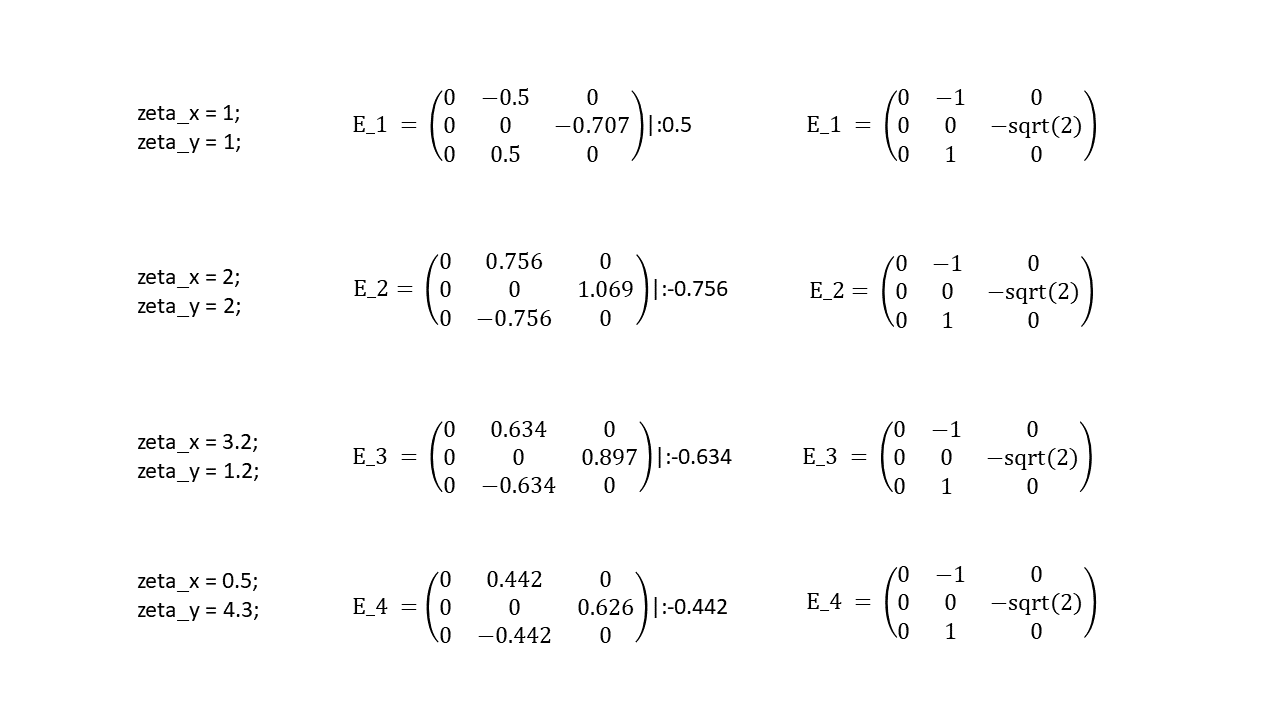
\includegraphics[width=1.\linewidth]{images/EMatrizen.png}
%	\captionof{figure}{Die essentiellen Matrizen sind bei jeder Auflösung, die gewählt wurden immer Vielfache voneinander} 
%\end{minipage}\\ \\

Bei der Rekonstruktion der externen Kamerparameter ergibt sich daraus stehts die selbe Matrix für $P'$. Was wie gezeigt daran liegt, dass sich geometrisch nichts ändert, sondern lediglich die skalierung der Koordinatenwerte der Bildpunkte und somit auch eine Skalierung der Einträge in $F$ und $E$, welche aber ebenfalls als Skaleninvariant definiert sind\cite{HZ}. Die Ergebnisse der darauffolgenden Szenenrekonstruktionen, der einzelnen Szenen zeigt, dass sich immer die selbe Szene ergibt, welche mit der eigens aufgebauten Szene übereinstimmen.\\


\begin{minipage}{\linewidth}
	\centering
	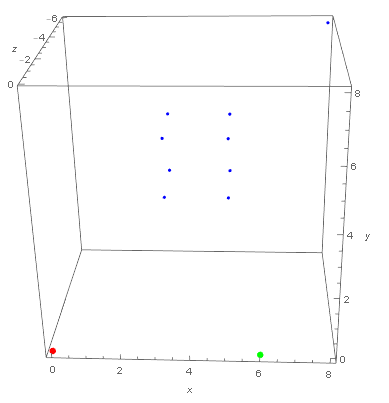
\includegraphics[width=0.5\linewidth]{images/DifferentAufloesungRekonstructedScene.png}
	\captionof{figure}{Die rekonstruierten Szenenpunkte und Kamerapositionen bleibt auch bei unterschiedlichen Auflösungen die selben} 
\end{minipage}\\ \\

Die Behauptung, dass die Auflösung der Kamera bei dem in dieser Arbeit gewählten Workflow für die Rekonstruktion der Szene keine Auswirkung hat, kann für das Minimalbeispiel bestätigt werden. \\







	
		% C2 - example 2
		\chapter{Reelle Rekonstruktion}
\label{sec:real} 

Der entwickelte Szenenrekonstrukionsalgorithmus wird im Folgenden anhand eines realen Stereoaufbaus getestet. Anders als bei den synthetischen Bilddaten im Beispiel zuvor, muss beim arbeiten mit reellen Stereobildern mit einer Fehleranfälligkeit der Bilddaten gerechnet werden. Liegt beispielsweise bei der Bestimmung von korrespondierenden Punkten eine Ecke zwischen zwei Pixel, so kann optisches Rauschen, welches in realen Aufnahmen präsent ist, dazu führen dass die Ecke in gleichen Bildern an verschiedenen Pixel erkannt wird. Diese Abweichung der Punktekorrespondenz führt dazu, dass die in Kapitel \ref{sec:EpiolarContraints} definierten epipolaren Bedingungen nicht zur Gänze mehr erfüllt werden. In diesem Kapitel wird Hauptsächlich darauf eingegangen, welche Auswirkungen diese Ungenauigkeiten auf die Bestimmung der Fundamentalmatrix, der essentiellen Matrix, der extrinsischen Kameraparameter und der anschließenden Rekonstruktion der Szene durch Triangulierng haben und wie man ihnen entgegenwirken kann. In Abbildung \ref{fig:ArbeitsProzessReell}, ist der Arbeitsprozess für den reellen Fall zu sehen. Der Ablauf im Allgemeinen bleibt beständig.

%Hierzu wurde der Ursprüngliche Algorithmus um bestimmte Funktionen erweitert, welche im Verlauf des Kapitels genau erläutert werden. Abbildung \ref{fig:ArbeitsProzessReell} zeigt den Ablauf für die Reelle Rekonstruktion. \\
%
%Bildfehler genauer beschreiben und lösungsansatz skizzieren

\begin{figure}[!htb]
	\centering
	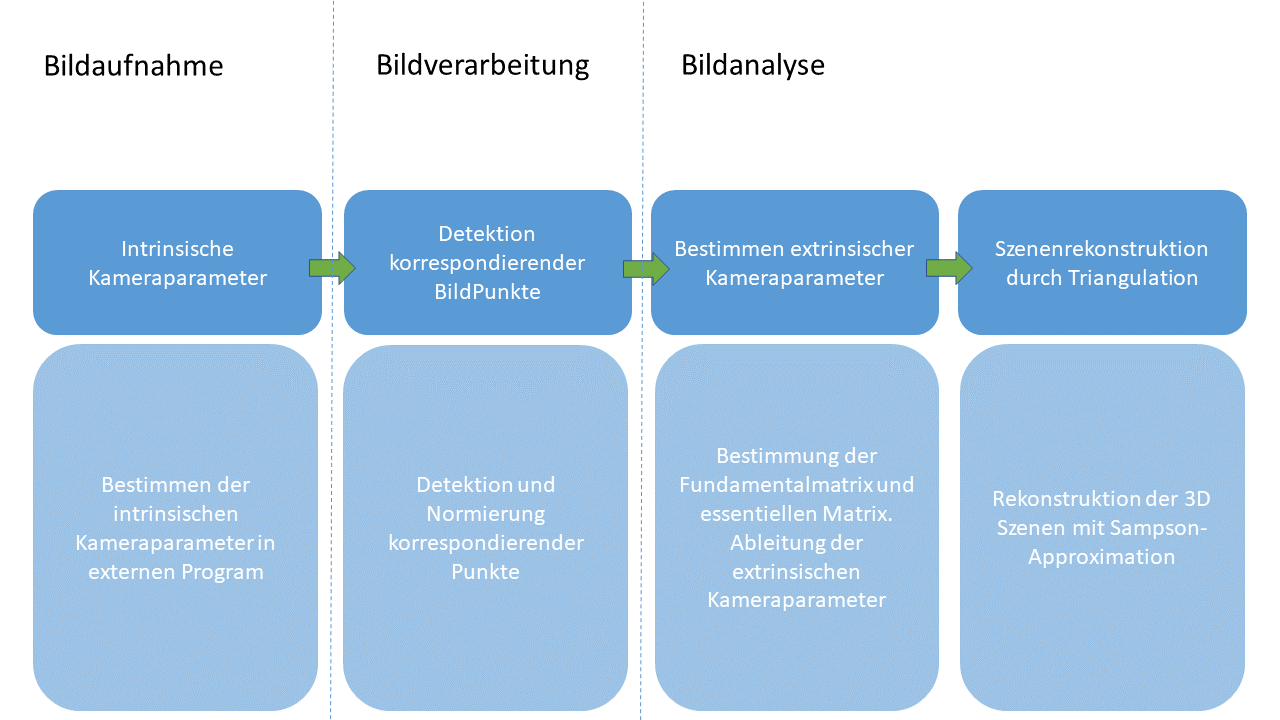
\includegraphics[width=1.\linewidth]{images/NEU_real_Arbeitsprozess.png}
	\caption[Ablaufdiagramm für die reelle Rekonstruktion]{Ablaufdiagramm für die reelle Rekonstruktion}
	\label{fig:ArbeitsProzessReell}
\end{figure}

%\begin{minipage}{\linewidth}
%	\centering
%	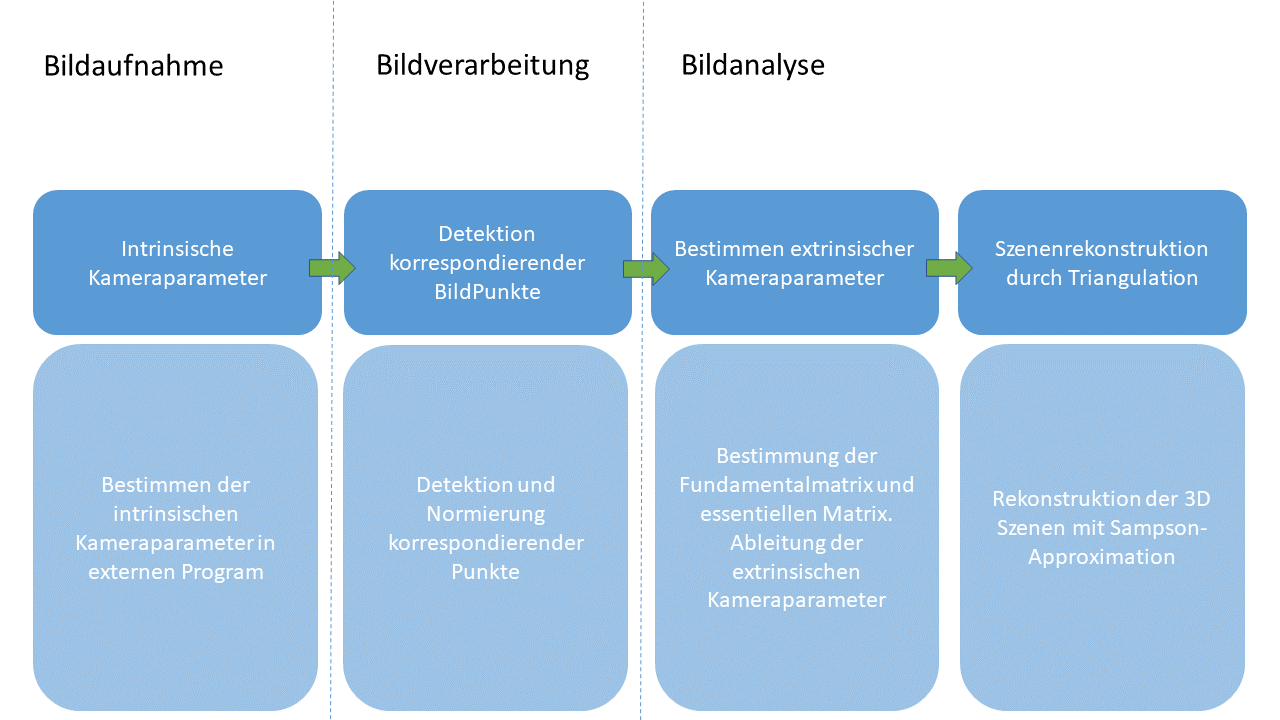
\includegraphics[width=1.\linewidth]{images/NEU_real_Arbeitsprozess.png}
%	\captionof{figure}{Ablaufdiagramm für die reelle Rekonstruktion}
%	\label{fig:ArbeitsProzessReell}
%\end{minipage}\\ \\

Zu Beginn wird der Stereoaufbau vorgestellt. Danach folgt die Korrespondenzanalyse, in welcher zwei Möglichkeiten aufgeführt werden, wie Punktekorrespondenzen aus den Stereoaufnahmen gewonnen werden können. Der Normierte-Acht-Punkt-Algorithmus, stellt eine für reale Bilddaten leicht veränderte Fassung des bereits bekannten Acht-Punkt-Algorithmus vor. Mit dessen Hilfe ist es möglich die Auswirkungen der Abweichungen in den Punktekorrespondenzen auf ein Minimum zu reduzieren. Nach der Bestimmung der Fundamentalmatrix durch den Normierten-Acht-Punkt-Algorithmus, wird diese auf ihre Gültigkeit kontrolliert. Hierzu werden vor allem die Singulärwerte der Fundamentalmatrix genauer betrachtet und welche Auswirkungen sie auf die Epipolargeometrie haben. Als nächstes wird die aus der Fundamentalmatrix bestimmte essentielle Matrix überprüft. Auch hier wird auf die Eigenschaften der Singulärwerte der essentiellen Matrix eingegangen.
\pagebreak

Danach wird eine Triangulierungsmethode nach \textit{Hartley \& Zisserman} \cite{HZ} vorgestellt, die über ein Näherungsverfahren eine Triangulation zwischen ungenauen korrespondierenden Punkten ermöglicht. Der letzte Abschnitt des Kapitels befasst sich dann mit der reellen Rekonstruktion bei unterschiedlichen Kameraauflösungen. \\



%Zunächst wird der Stereoskopische Aufbau kurz erläutert. 
%
%Der selbe Arbeitsprozess soll nun auch auf ein Realbeispiel mit Bildern zweier Kameras durchgeführt werden.
%
%Für die Kalibrierung der intrinsischen Kameraparameter wird auf ein externes Programm zurückgegriffen.
%
%Der Arbeitsprozess wird ähnlich dem des Minimalbeispiels ablaufen\\
%
%Auf bestimmte besonderheiten wird eingegangen, da reele Daten Fehleranfällig sind, genau so wie die detektion der korrespondierenden Bildpunkte
%
%
%Für die Stereoaufnahmen wurden die halbformat Kamera Canon 60 D und die Vollformatkamera 6D verwendet. Die Bilder wurden zunächst mit beiden Kameras bei selber Auflösung. Später wurden auch noch aufnahmen mit unterschiedlichen Auflösungen gemacht und ebenfalls die Stereoanalyse auf die Bildpaare angewandt.  \\


\section{Stereoaufbau}


Für die Stereobildaufnahme wurde eine Szene vor zwei nebeneinander platzierten Kameras aufgebaut. Beide Kameras wurden auf die Szene gerichtet. Abbildung \ref{fig:StereoaufbauReal} zeigt den entstandenen Stereoaufbau.\\

%Die räumliche Orientierung und Position von $C'$ wird also relativ zu $C$ berechnet und auch die Szene wird davon ausgehend, dass $C$ als Projektionsmatrix $P=[I|0]$ besitzt.

% dass sie leicht zueinander hin gedreht waren. Da die Canon 60D eine halbformatkamera ist, wurde sie weiter hinten als die Canon 6D positioniert. Somit konnte ungefähr der selbe Bildausschnitt der Szene mit beiden Kameras aufgenommen werden.\\



\begin{figure}[!htb]
	\centering
	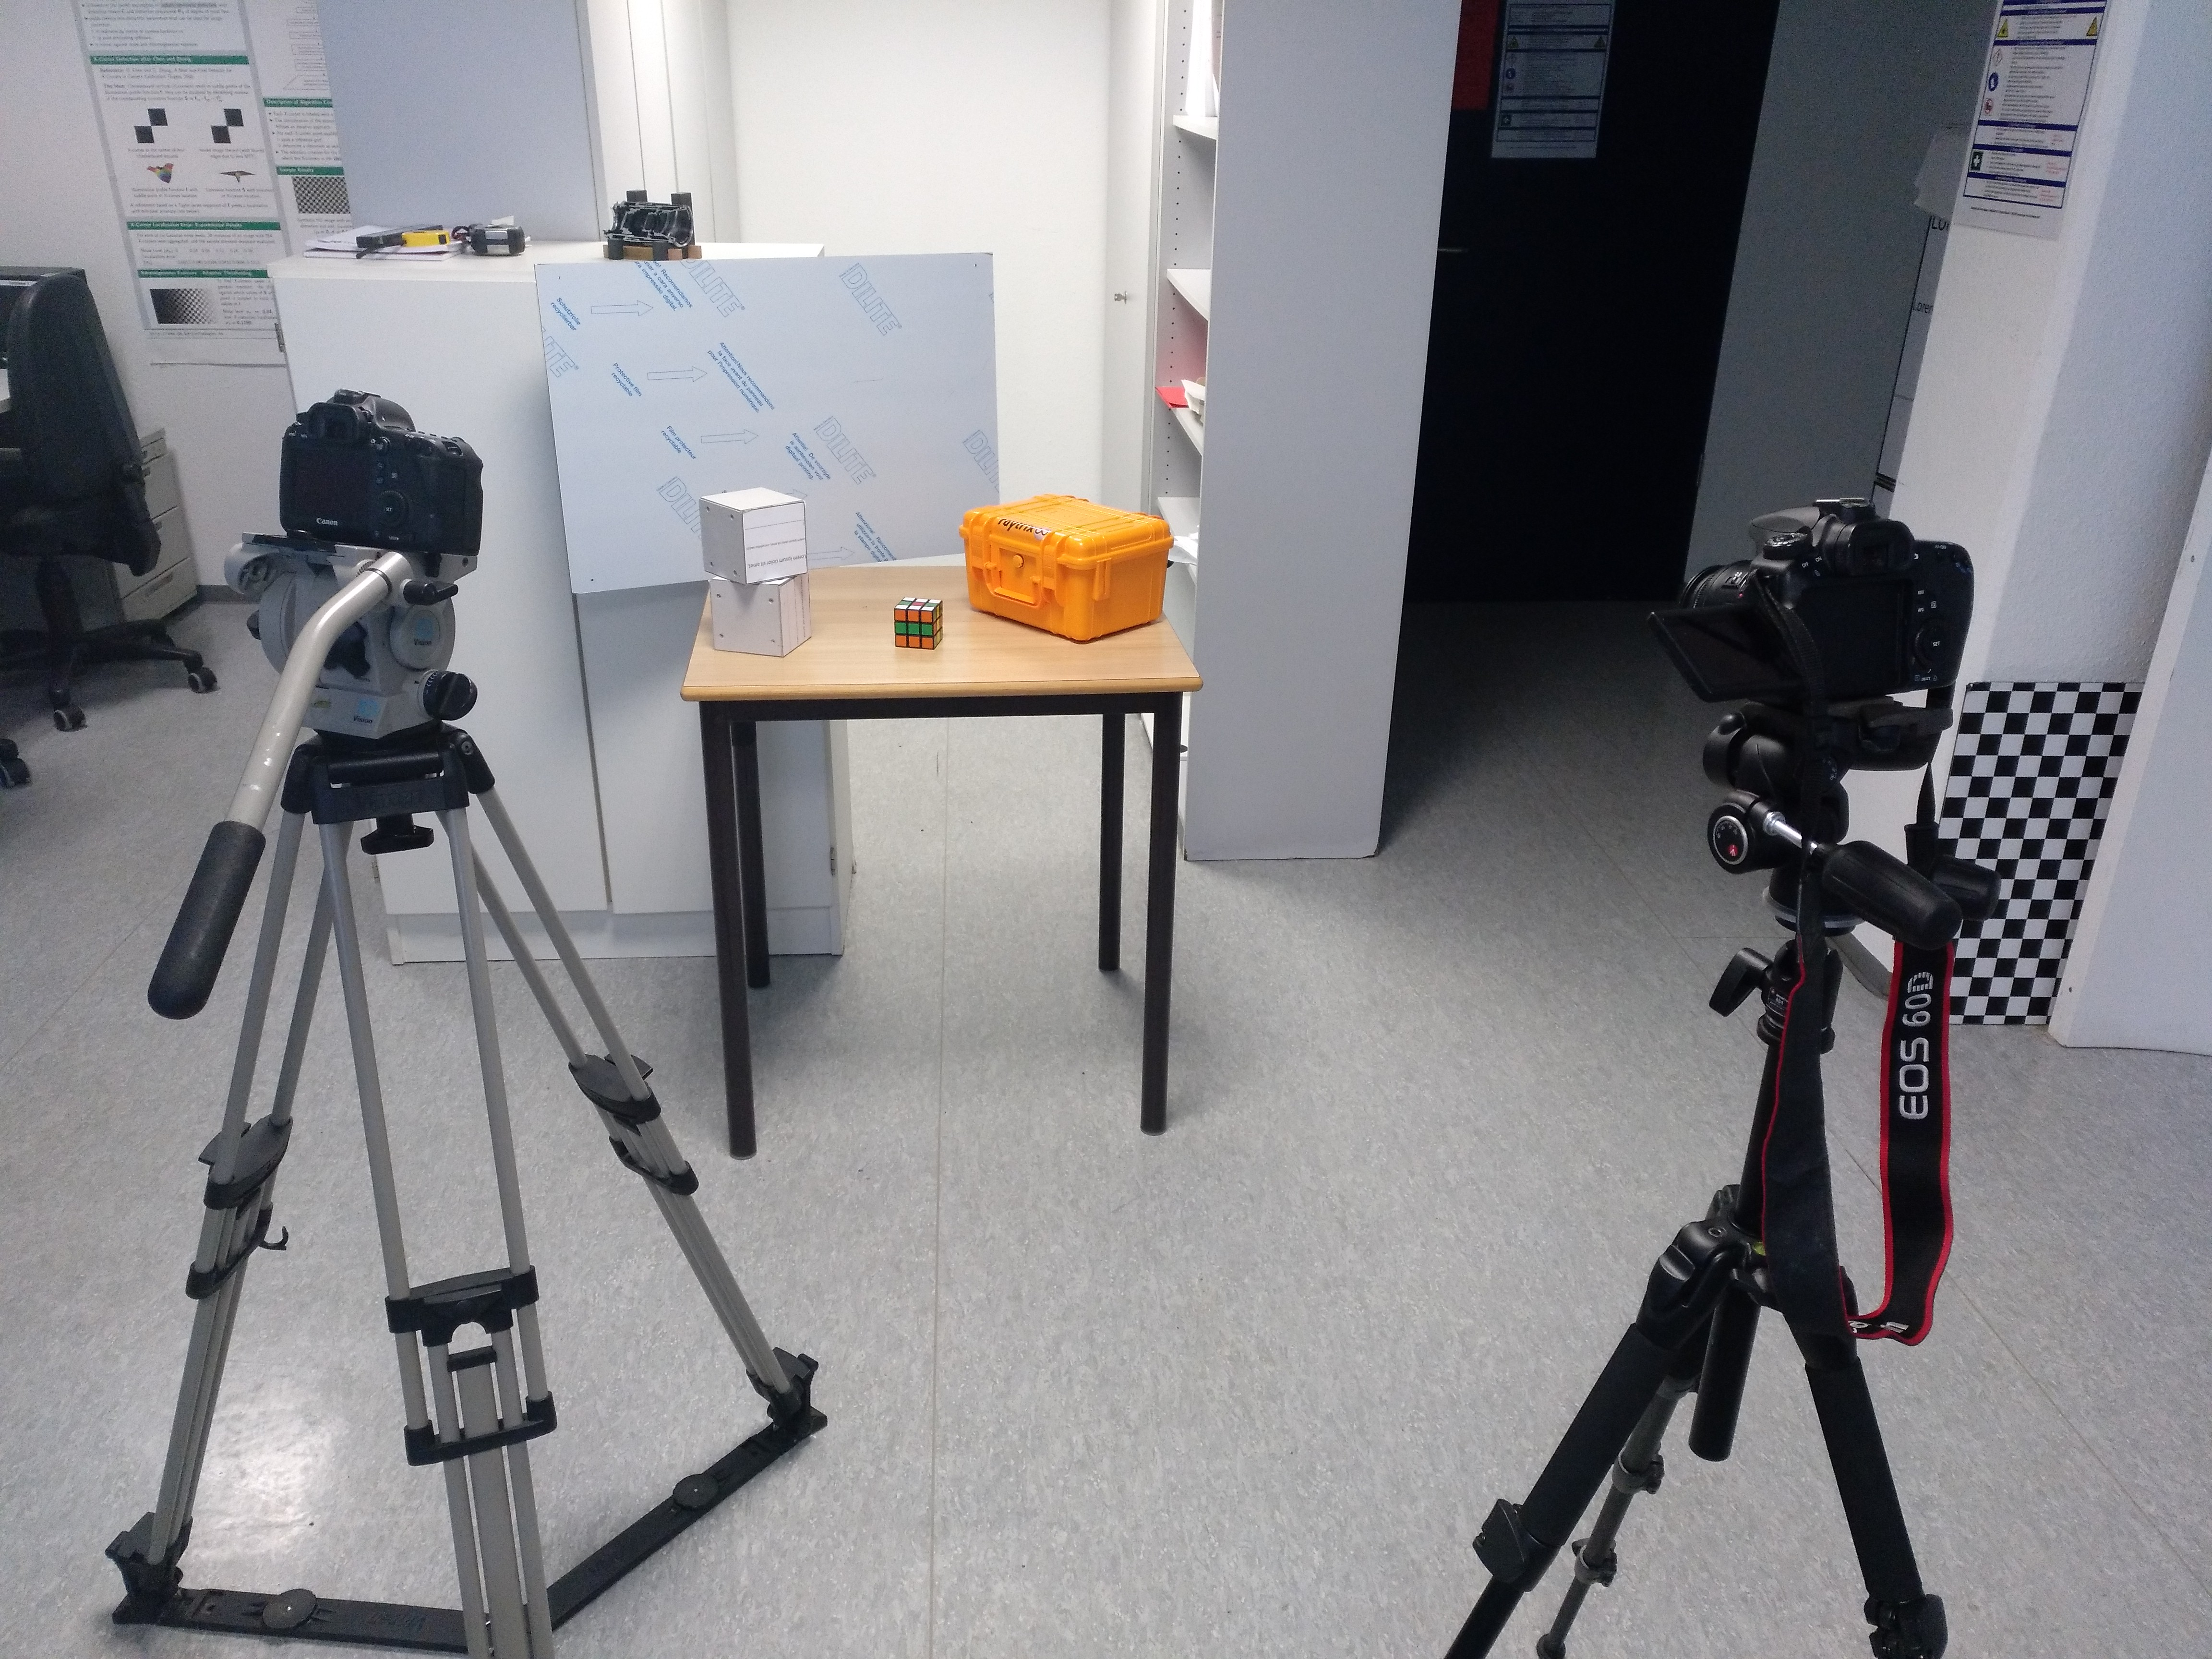
\includegraphics[width=.7\linewidth]{images/SetUpSameResolution.jpg}
	\caption[Stereoaufbau im Überblick]{Kamera eins $C$ befindet sich auf dem Bild links, Kamera zwei $C'$ befindet sich rechts im Bild. Auf dem Tisch zwischen den Kameras ist die in den Abbildungen \ref{fig:SurfLinks} und \ref{fig:SurfRechts} abgebildete Szene zu sehen. Beide Kameras sind auf die Szene gerichtet.}
	\label{fig:StereoaufbauReal}
\end{figure}


%\begin{minipage}{\linewidth}
%	\centering
%	\includegraphics[width=.7\linewidth]{images/SetUpSameResolution.jpg}
%	\captionof{figure}{Szenenaufbau: Die Canon 60D befindet sich in dieser Abbildung auf der linken Seite, die Canon 60 D auf der rechten. Auf dem Tisch zwischen den Kameras ist die in den Abbildungen 6.1 und 6.1 abgebildete Szene zu sehen. Beide Kameras sind zu Szene hin gedreht.}
%	\label{fig:StereoaufbauReal}
%\end{minipage}\\

Die auf Abbildung \ref{fig:StereoaufbauReal} zu sehende linke Kamera wurde als primäre Kamera definiert. Die extrinsischen Kameraparameter für $C'$, werden dahingehend realiv zu $C$ bestimmt werden. Das Kamerakoordinatensystem $(C,\beta)$ entspricht somit gleich dem Weltkoordinatensystem $(O,\delta)$. Kamera zwei mit $(C',\beta')$ befindet sich auf der Abbildung rechts. Für beide Kameras wurden in einem externen Programm die intrinsischen Kameraparameter $K$ und $K'$ bestimmt. An den Stereoaufnahmen der Szene wird dann eine Korrespondenzanalyse durchgeführt.   

\section{Korrespondenzanalyse}


Für die Detektion von Punktekorrespondenzen bei Stereoaufnahmen einer dreidimensionalen Szene wurde eine bereits existierende Funktion von Mathematica genutzt\cite{Mathematica}. Die Funktion basiert auf dem Prinzip eines SURF-Algorithmus. SURF ist die Kurzform für \textit{Speeded Up Robust Features} und ist ein Rotations- und Skaleninvarianter Punkte Detektor und Deskriptor\cite{SURF,SIFTSURF}. Es werden Punkte an markanten Stellen in beiden Bildern detektiert, wie beispielsweise Eckpunkte oder Kanten. Die Umgebung eines jeden gefundenen Punktes wird durch einen Merkmalsvektor, dem Deskriptor, beschrieben. Die Deskriptoren beider Bilder werden abgeglichen und gleiche Punkte werden als korrespondierende Punkte gekennzeichnet\cite{SURF,SIFTSURF}. Die Abbildungen \ref{fig:SurfLinks} und \ref{fig:SurfRechts} zeigen die Ergebnisse nach der Anwendung des SURF-Algorithmus auf das Stereobildpaar. 
\pagebreak

Eine eigens implementierte alternative für die Korrespondenzanalyse zwischen Stereoaufnahmen eines zweidimensionalen Schachbretts wird in Kapitel \ref{sec:schachbrettAlg} vorgestellt.  


%	\minipage{0.48\textwidth}
%	\includegraphics[width=\linewidth]{images/Points3DSceneLeft.png}
%	\caption{Aufnahme der Canon 6D von links}
%	\label{fig:awesome_image1}
%	\endminipage\hfill
%	\minipage{0.48\textwidth}
%	\includegraphics[width=\linewidth]{images/Points3DSceneRight.png}
%	\caption{Aufnahme der Canon 60D von rechts}
%	\label{fig:awesome_image2}
%	\endminipage\hfill
%\end{figure}
\begin{figure}[!htb]
	\minipage{0.48\textwidth}
	\includegraphics[width=\linewidth]{images/PointsDetectedLeft.png}
	\caption[Aufnahme von Kamera $C$]{Aufnahme von Kamera $C$}
	\label{fig:SurfRechts}
	\endminipage\hfill
	\minipage{0.48\textwidth}
	\includegraphics[width=\linewidth]{images/PointsDetectedRight.png}
	\caption[Aufnahme von Kamera $C'$]{Aufnahme von Kamera $C'$}
	\label{fig:SurfLinks}
	\endminipage\hfill
%	\caption{Die mit dem \textit{SURF}-Algorithmus gefundenen Punkte sind mit den gelben Ziffern im Bild gekennzeichnet. Abbildung a zeigt das Bild von $C$, die Abbildung b zeigt das Bild von $C'$}
\end{figure}
%\pagebreak

Die mit dem \textit{SURF}-Algorithmus gefundenen Punkte sind mit den gelben Ziffern in den Abbildungen \ref{fig:SurfLinks} und \ref{fig:SurfRechts} gekennzeichnet. Die Abbildung \ref{fig:SurfLinks} zeigt das Bild von $C$, die Abbildung \ref{fig:SurfRechts} zeigt das Bild von $C'$.\\

Die Detektion von Punktekorrespondenzen mit Detektionsalgorithmen, wie beispielsweise dem angewendeten SURF-Algorithmus, können immer Fehler und Abweichungen mit sich bringen. Die Ursprünge der Fehler können sowohl durch den Algorithmus als auch durch Fehler, wie Bildrauschen, in den Aufnahmen selbst entstehen. Diese Fehler wirken sich sowohl auf die Bestimmung der Abbildungsvorschriften $F$ und $E$ aus und somit auch auf die Genauigkeit der Szenenrekonstruktion\cite{HZ}. Im Folgenden werden sowohl die Fehler als auch Methoden für deren Minimierung vorgestellt.

\section{Normierter-Acht-Punkt-Algorithmus}

Trotz das der Acht-Punkt-Algorithmus eine einfache Methode zur Bestimmung der Fundamentalmatrix bietet, ist er sehr instabil sobald Fehler wie Ungenauigkeiten in Punktekorrespondenzen  auftreten\cite{HZ,Brooks}.\\

Die Ausmaße der Fehler lässt sich anhand der Kondition der Koeffizientenmatrix $A$ genauer feststellen. Als Kondition wird die Abhängigkeit der Lösung eines Problems von der Störung der Eingangsdaten beschrieben\cite{HZ8,ConditionNumber,Manocha}. Die Kondition lässt sich durch Bestimmung des kleinsten Eigenvektors der Matrixmultiplikation der Koeffizientenmatrix $A$ mit ihrer Transponierten $A^T$ herausfinden. Die Matrix $AA^T$ wird in die Matrizen $UDU^T$ zerlegt, wobei $U$ eine orthogonale und $D$ eine diagonale Matrix ist. Die Diagonaleinträge von $D$ sind in einer nicht ansteigenden Reihenfolge, woraus resultiert, dass der kleinste Singulärwert von $D$ mit der letzten Spalte von $U$ korrespondiert. Die letzte Spalte von $U$ is gleich dem kleinsten Eigenvektor von $AA^T$\cite{HZ8,ConditionNumber}. Wird angenommen, dass $AA^T$ eine 9 $\times$ 9- Matrix ist, so ergeben die Diagonaleinträge $d_1/d_9$ den Wert der Kondition. Je größer die Kondition ist, desto größer wirken sich schon kleinste Abweichungen der reinkommenden Bilddaten, auf die aus $A$ bestimmte Matrix $F$ aus. Erkenntlich wird eine schlechte Kondition dann zum Beispiel an einem Ungleichgewicht der Matrixeinträge von $F$\cite{HZ8}. Das bedeutet, dass sich die Matrixeinträge stark in ihren Größeneinheiten unterscheidet. \\

\begin{gather}
	F = \begin{pmatrix}
		10^{-8}&10^{-6}&10^{-4}\\
		10^{-7}&10^{-8}&10^{-3}\\
		10^{-4}&10^{-3}&10^{-2}\\
	\end{pmatrix}
\end{gather}.

Die epipolare Bedingung mit $m'^T_{\sigma'}Fm_\sigma = 0$ errechnet schon bei kleinste Abweichungen der Punktekorrespondenzen große Fehler. Die schlechte Kondition liegt laut $Hartley \& Zisserman$ an der weitflächigen Verteilung der homogenen Bildkoordinaten im Raum. Die heutigen Kameras können Bilder mit bis zu mehreren tausend Pixel aufnehmen. Ein Bildpunkt kann somit beispielsweise wie folgt aussehen.

\begin{gather}
	m_\sigma = \begin{pmatrix}
		1150\\2193\\1
	\end{pmatrix}
\end{gather}

$m_{\sigma\, x}$ und $m_{\sigma\, y}$ liegen in einem Bereich der sich um mehr als 1000 Pixel unterscheidet. Das bedeutet, dass sich die ersten beiden Koordinateneinträge um einen viel größeren Zahlenbereich befinden als ihre dritte Komponente. Um die Kondition möglichst klein zu halten, werden die Bildkoordinaten beider Bilder normiert\cite{HZ8,Brooks}. Normierte Koordinaten befinden sich in einem ausgeglicheneren Wertebereich und liegen nicht mehr weit verteilt im Raum\cite{HZ8}. Ihre Einträge entsprechen dem Folgenden Beispiel

 \begin{gather}
 	m_\sigma = \begin{pmatrix}
 		1.5\\1.193\\1
 	\end{pmatrix}
 \end{gather}.

Die Einträge der entstehende Fundamentalmatrix haben dann die Form

\begin{gather}
	F = \begin{pmatrix}
		10^{-3}&10^{-2}&10^{-2}\\
		10^{-2}&10^{-3}&10^{-2}\\
		10^{-2}&10^{-2}&10^{-2}\\
	\end{pmatrix}
\end{gather}.

Das hat zur Folge, dass die epipolare Bedingung  weniger stark auf ungenaue Punktekorrespondenzen reagiert. Die in Literaturquellen, vorgeschlagene Methode zur Normierung besteht darin den Schwerpunkt aller Punkte in den Ursprung des Sensorkoordinatensystems zu verschieben und die Bildpunkt so zu skalieren, dass ihr durchschnittlicher Abstand zum Ursprung $\sqrt{2}$ beträgt\cite{HZ,Ferid,Brooks}.\\


Für die Normierung wird pro Bild eine Transformationsmatrix $T$ und $T'$ definiert. Die Matrizen beinhalten sowohl eine Skalierung als auch eine Translation. Die Bestimmung der Matrix $T$ wird im Folgenden aufgezeigt. Zuerst wird der Schwerpunkt $s$ mit $s=\begin{pmatrix}
s_x\\
s_y
\end{pmatrix}$ der Punktemenge $p_n$ mit $p_n = \begin{pmatrix}
p_{nx}\\
p_{ny}
\end{pmatrix}$ berechnet, indem der Mittelwert aller Punkte $p_n$ berechnet wird.

\begin{gather}
	\begin{pmatrix}
		s_x\\
		s_y
	\end{pmatrix} = \frac{1}{n} \sum_{i = 1}^{n} \begin{pmatrix}
	p_ix\\
	p_iy
\end{pmatrix}
\end{gather}

Danach wird $s$ in den Ursprung verschoben. Die Punkte $x_n$ werden ebenfalls um den Wert von $s$ verschoben $x'_n = x_n - s$. Der Mittelwert aus den um $s$ verschobenen Punkten $x'_n$ ergibt den neuen Schwerpunkt $s_0$ im Koordinatenursprung. Als nächstes wird die Distanz jedes Punktes von $x'_n$ zu $s_0$ berechnet und der Mittelwert aller Distanzen, hier mit $d$ bezeichnet, berechnet. Die Matrix $T$ und $T'$ haben dann die folgende Form:

\begin{gather}
	T = \begin{pmatrix}
		\frac{\sqrt{2}}{d}&0&-s_x\\
		0&\frac{\sqrt{2}}{d}&-s_y\\
		0&0&1
	\end{pmatrix}\\
	T' = \begin{pmatrix}
	\frac{\sqrt{2}}{d'}&0&-s'_x\\
	0&\frac{\sqrt{2}}{d'}&-s'_y\\
	0&0&1
\end{pmatrix}
\end{gather}

Die originalen Bildpunkte des Stereobildpaares, werden mit den Matrizen $T$ und $T'$ verrechnet. Mit den Normierten Bildkoordinaten wird dann mit dem Acht-Punkte-Algorithmus eine Fundamentalmatrix $\hat{F}$ bestimmt\cite{HZ,HZ8,Ferid,Brooks}. Ist $\hat{F}$ aus den normierten Koordinaten bestimmt, wird sie mit $T$ und $T'$ wieder denormalisiert.

\begin{gather}
	F = T'^T\hat{F}T
\end{gather}



\subsection{Singularität der Fundamentalmatrix}
\label{sec:SingularityOfF}

Die aus den Punktekorrespondenzen bestimmte Fundamentalmatrix muss eine singuläre Matrix mit Rang 2 sein\cite{HZ,ZZGXr,Ferid}. Die Singularität der Fundamentalmatrix sorgt zum einen dafür das ihr rechter und linker Kern jeweils eine eindeutige Lösung für den Epipol des jeweiligen Bildes ergibt und die Epipolarlinien, welche mit $l = Fm_\sigma$ und $l' = F^Tm'_{\sigma'}$ berechnet werden, auch alle durch diese Epipole verlaufen\cite{HZ}. Durch Ungenauigkeiten in korrespondierenden Bildpunkten kann es dazu kommen, dass die aus dem Normierten-Acht-Punkt-Algorithmus bestimmte Fundamentalmatrix $\hat{F}$ in ihrem Rang steigt und somit keine singuläre Matrix mehr ist. Matrizen sind singulär, wenn sie keine Inverse besitzen, was durch as verschwinden der Determinante nachgewiesen werden kann\cite{FormelsammlungMatrizen}. Die Determinanten von $\hat{F}$ muss Null sein, damit sie eine singuläre Matrix ist.\\

Ist $\hat{F}$ durch den erhöhten Rang keine singuläre Matrix, so ergeben der linke und der rechte Kern von $\hat{F}$ keine eindeutigen Lösungen mehr für $e$ und $e'$ und die Epipolarlinien in beiden Bildern verlaufen dementsprechend auch nicht mehr durch genau einen Punkt, wie man in den Abbildungen \ref{fig:NoEpipoleWithF1} und \ref{fig:NoEpipoleWithF2} erkennen kann. Die Abbildungen bilden Epipolarlinien aus dem Stereobildpaar \ref{fig:SurfRechts} und \ref{fig:SurfLinks} ab. Die Ursache des erhöhten Ranges von $\hat{F}$ ist in ihren Singulärwerten von $F$ zu finden.\\


%
%irgendwie sagen dass es durch verunreinigte daten zu fehlern im constraint kommt und die Fundamentalmatrix im Rang steigt.
%
%Die Fundamentalmatrix ist eine singuläre-Matrix und ist somit eine Matrix von Rang zwei. Di
%
%wird die Fundamentalmatrix durch eine Singulärwertszerlung von $A$ geschätzt, ist die Chance sehr hoch, dass das Ergebnis für $\hat{F}$ eine Matrix von Rang 3 ist. Sollte dies der Fall sein gehen die Epipolarlinien der Bilder nicht mehr durch genau einen Punkt, wie man in den Abbildungen 6.5 und 6.6 erkennen kann. Diese bilden Epipolarlinien in einem Stereobildpaar ab.\\

\begin{figure}[!htb]
	\minipage{0.46\textwidth}
	\includegraphics[width=\linewidth]{images/L_F_no_Constraint.png}
	\caption[Epipolarlinien $C$ ohne Singularität]{Epipolarlinien ohne \textit{Epipolar-constraint} im Bild der Canon 6D}
	\label{fig:NoEpipoleWithF1}
	\endminipage\hfill
	\minipage{0.46\textwidth}
	\includegraphics[width=\linewidth]{images/LPrime_PC2_F_no_Constraint.png}
	\caption[Epipolarlinien $C'$ ohne Singularität]{Epipolarlinien ohne \textit{Epipolar-constraint} im Bild der Canon 60D}
	\label{fig:NoEpipoleWithF2}
	\endminipage\hfill
	%	\caption{Die mit dem \textit{SURF}-Algorithmus gefundenen Punkte sind mit den gelben Ziffern im Bild gekennzeichnet}
\end{figure}

%Um eine gültige Fundamentalmatrix für den weiteren Arbeitsprozess zu generieren, kommt hier ein sogenannter \textit{singularity constraint} zum Einsatz.

Um mit dem Algorithmus weiter verfahren zu können, muss die Singularität in der noch normierten Fundamentalmatrix $\hat{F}$ erzwungen werden\cite{HZ}. Hierfür wird eine Singulärwertzerlegung an $\hat{F}$ durchgeführt, so dass $\hat{F}$ in $\hat{F} = U\Sigma V^T$ zerlegt wird. $\Sigma$ beinhaltet in einer Diagonalmatrix die Singulärwerte $D = \text{diag}(r,s,t)$. Die Diagonaleinträge erfüllen die Bedingung, dass $r \geq s \geq t $ gilt. Damit $\hat{F}$ zu einer singulären Matrix wird, muss für die Diagonaleinträge jedoch gelten, dass  $\Sigma = \text{diag}(r,s,0)$ ist. Diese Bedingung wird erzwungen, indem der letzte Eintrag $t$ auf $t = 0$ gesetzt wird. Die so modifizierte Fundamentalmatrix mit $\bar{F} = U\text{diag}(r,s,0)V^T$ wird dann wieder zusammengesetzt. Die Fundamentalmatrix $\bar{F}$ besitzt jetzt einen Rang 2 und ist singulär\cite{HZ}. $\bar{F}$ minimiert die Frobenius Norm $\parallel \hat{F} -\bar{F} \parallel$ und ist die nächste zum ursprünglichen $F$ liegende singuläre Matrix von Rang 2\cite{HZ,HZ8,FormelsammlungMatrizen}. \\

Werden aus $\bar{F}$ der rechte und linke Kern bestimmt, so ergeben sich eindeutige Lösungen für $e$ und $e'$ und die Epipolarlinien $l$ und $l'$ verlaufen jeweils durch ihre entsprechenden Epipole\cite{HZ}. Die Abbildungen \ref{fig:EpipoleWithF1} und \ref{fig:EpipoleWithF2} zeigen die Auswirkung der erzwungenen Singularität von $F$ auf dem Stereobildpaar \ref{fig:SurfRechts} und \ref{fig:SurfLinks}. Die Abbildungen \ref{fig:EpipoleWithF1Denorm} und \ref{fig:EpipoleWithF2Denorm} zeigen die selben Epipolarlinien nur ist $\bar{F}$ mit $T$ und $T'$ denormalisiert worden.\\



% Zu aller erst wird eine Singulärwertszerlegung an $F$ durchgeführt, so dass $\hat{F}$ in $\hat{F} = UDV^T$ zerlegt wird. $D$ beinhaltet in einer diagonalen Matrix die Singulärwerte $D = \text{diag}(r,s,t)$, welche die Bedingung $r \leq s \leq t $ erfüllen. 
% 
% Um nun den \textit{singularity-constraint} in $\hat{F}$ zu erzwingen, wird der letzte Singulärwert $t = 0$ gesetzt, so dass am Ende dasteht $D = \text{diag}(r,s,0)$. Danach werden die Matrizen $UDV^T$, wobei $D$ nun die modifizierten Singulärwerte beinhaltet, wieder zu $\hat{F}$ multipliziert. Die jetzt resultierende Fundamentalmatrix $\hat{F}$ besitzt den Rang 2. Der rechte und linke Kern ergeben wieder die Epipole und die Epipolarlinien verlaufen wieder durch eben diese Epipole. Die Abbildungen 6.7 und 6.8 zeigen die selben Epipolarlinien wie in 6.5 und 6.6 nachdem der \textit{singularity-constraint} in $\hat{F}$ erzwungen wurde. Die somit entstandene Matrix $\hat{F}$, ist die laut Frobenius norm, nächste zum ursprünglichen $\hat{F}$\cite{HZ}.

%Jetzt erst erfolgt die zuvor erwähnte denormierung von $\hat{F}$ durch $T$ und $T'$. Die Abbildungen 6.9 und 6.10 zeigen die Epipolarlinien im Originalbild mit denormierten Koordinaten.


\begin{figure}[!htb]
	\minipage{0.46\textwidth}
	\includegraphics[width=\linewidth]{images/L_PC1_F_Constraint.png}
	\caption[Epipolarlinien in $C$ aus singulärer Fundamentalmatrix]{Die Abbildung zeigt, dass die Epipolarlinien auf der Aufnahme von $C$, nach dem Erzwingen der singularität in der normierten $\hat{F}$, alle durch den Epipol $e$ verlaufen}
	\label{fig:EpipoleWithF1}
	\endminipage\hfill
	\minipage{0.46\textwidth}
	\includegraphics[width=\linewidth]{images/LPrime_PC2_F_Constraint.png}
	\caption[Epipolarlinien in $C'$ aus singulärer Fundamentalmatrix ]{Die Abbildung zeigt, dass die Epipolarlinien auf der Aufnahme von $C'$, nach dem Erzwingen der singularität in der normierten $\hat{F}$, alle durch den Epipol $e'$ verlaufen}
	\label{fig:EpipoleWithF2}
	\endminipage\hfill
	%	\caption{Die mit dem \textit{SURF}-Algorithmus gefundenen Punkte sind mit den gelben Ziffern im Bild gekennzeichnet}
\end{figure}

\begin{figure}[!htb]
	\minipage{0.46\textwidth}
	\includegraphics[width=\linewidth]{images/L_PC1_F_Constraint_denormalized.png}
	\caption[Epipolarlinien in $C$ aus singulärer denormalisierter Fundamentalmatrix]{Die Abbildung zeigt die Epipolarlinien in $C$ nachdem die Fundamentalmatrix $\bar{F}$ mit $F = T'\bar{F}T$ denormalisiert wurde}
	\label{fig:EpipoleWithF1Denorm}
	\endminipage\hfill
	\minipage{0.46\textwidth}
	\includegraphics[width=\linewidth]{images/LPrime_PC2_F_Constraint_denormalized.png}
	\caption[Epipolarlinien in $C$ aus singulärer denormalisierter Fundamentalmatrix]{Die Abbildung zeigt die Epipolarlinien in $C'$ nachdem die Fundamentalmatrix $\bar{F}$ mit $F = T'\bar{F}T$ denormalisiert wurde}
	\label{fig:EpipoleWithF2Denorm}
	\endminipage\hfill
	%	\caption{Die mit dem \textit{SURF}-Algorithmus gefundenen Punkte sind mit den gelben Ziffern im Bild gekennzeichnet}
\end{figure}

\pagebreak

\subsection{Singulärwerte der essentiellen Matrix}

Die essentielle Matrix wird im entwickelten Algorithmus aus der Fundamentalmatrix $F$ bestimmt. Da zuvor die singularität von $F$ erzwungen wurde, ist die essentielle Matrix ebenfalls eine Matrix von Rang 2\cite{HZ}. Im synthetischen Beispiel wurde gezeigt, dass für die Bestimmung der extrinsischen Kameraparameter für $E$ gelten muss, dass für ihre Singulärwerte $\Sigma = \text{diag}(1,1,0)$ sind. \\

Die Ungenauigkeit der Punktekorrespondenzen, kann auf $E$ die Auswirkung haben, dass ihre Singulärwerte die Form $\Sigma = \text{diag}(a,b,c)$ mit $a \geq b \geq c$ annehmen. Eine Matrix gilt nur dann als essentielle Matrix, wenn zwei ihrer Singulärwerte gleich sind $(a = b)$ und für den dritten gilt $(c=0)$. Um diese Bedingung zu erzwingen, wird diejenige essentielle Matirix $\hat{E}$ gesucht, welche sich laut der Frobenius Norm am nächsten an der ursprünglichen $E$ befindet\cite{HZ,Ferid}. Diese Matrix lässt sich aus $E = U \Sigma V^T$ bestimmen, indem eine neue essentielle Matrix $\hat{E} = U \hat{\Sigma}V^T$ mit $\hat{\Sigma} = \text{diag}(\frac{a+b}{2},\frac{a+b}{2},0)$\cite{HZ} gebildet wird.\\

Nach erzwingen der singulären Bedingung $\hat{\Sigma} = \text{diag}(\frac{a+b}{2},\frac{a+b}{2},0)$, ist $E$ wieder eine gültige essentielle Matrix und der Algorithmus kann mit der Bestimmung der extrinsischen Kameraparameter, wie in Kapitel \ref{sec:minimal} gezeigt, fortfahren.\\

Das Erzwingen der singulären Bedingungen für $F$ und $E$ sind Näherungsverfahren, in welchen die Auswirkungen der Fehlerhaften Punktekorrespondenzen minimiert werden. Nur wenn $F$ und $E$ ihre singulären Bedingungen erfüllen, können die extrinsischen Kameraparameter bestimmt und die Szene rekonstruiert werden\cite{HZ}.

\section{Szenenrekonstruktion mit Sampson-Approximation}
\label{sec:sampson}

Aufgrund der Ungenauigkeit der korrespondierenden Punkte ist es nicht möglich die 3D-Objektpunkte durch einfache Rückprojektion der Bildpunkte zu rekonstruieren. Liegt der zu $m_\sigma$ korrespondierende Bildpunkt $m'_{\sigma'}$ nicht ganz genau auf der zu $m_\sigma$ korrespondierenden Epipolarlinie, so ist die in Kapitel \ref{sec:HFE} aufgestellte epipolare Bedingung aus Gleichung \ref{eq:Ep6} nicht mehr erfüllt. Durch einsetzten der detektierten korrespondierenden Punkte $m_\sigma$ und $m'_{\sigma'}$ in die Gleichung 

\begin{gather}
	m'^T_{\sigma'}Fm_\sigma = 0
\end{gather}

kommt ein Wert $\neq 0$ heraus. Je weiter der Wert von Null abweicht, desto ungenauer ist die Korrespondenz beider Bildpunkte. Dies führt dazu, dass sich bei der Rückprojektion die Linien der Bildpunkte $m_\sigma$ und $m'_{\sigma'}$ nicht im Raum treffen, sondern windschief zueinander liegen. Die Abbildungen \ref{fig:ProblemTraingulation} und \ref{fig:lFm} veranschaulichen die Konsequenz von ungenauen Punktekorrespondenzen.
%
%ist es bei den Fehlerhaften Bildkooridinaten nicht möglich die 3D-Szenenpunkte durch eine einfache Rückprojektion der der Bildpunkte zu einem Punkt im 3D-Raum zu erhalten. 
%
%sagen dass der epipolarconstraint nicht genau erfüllt wird
%
%Grund nennen und an bilder zeigen 
%Im letzten Schritt des Arbeitsprozesses, wird nun noch die Szenen mit Hilfe eines Triangulationsverfahrens rekonstruiert. Wie bereits im Kapitel \nameref{sec:minimal} erwähnt wurde, ist es bei den Fehlerhaften Bildkooridinaten nicht möglich die 3D-Szenenpunkte durch eine einfache Rückprojektion der der Bildpunkte zu einem Punkt im 3D-Raum zu erhalten. 
%
%liegt nur einer der beiden Bildpunkte $m$ oder $m'$ nicht hundert prozentig auf der jeweilgen korrespondierenden Epipolarlinie, so liegen die rückprojizierten Strahlen windschief im Raum. Das liegt daran, dass die Bildpunkte $m$ und $m'$ nicht den \textit{Epipolar-Constraint} $m'^T F m = 0$ erfüllen. Sprich die Gleichungen $m = PM$ und $m' = P'M$ können nicht erfüllt werden, da es kein $M$ gibt, dass für beide Gleichungen mit den momentanen $m$ und $m'$ gibt. Abbildung 6.11 veranschaulicht die Rückprojektion der Kamerazentren durch zwei Fehlerhafte Bildpunkte. 

\begin{figure}[!htb]
	\minipage{0.48\textwidth}
	\includegraphics[width=\linewidth]{images/problemTriangulation_beschriftet.png}
	\caption[Windschiefe Geraden]{a) Windschiefe Geraden}
	\label{fig:ProblemTraingulation}
	\endminipage\hfill
	\minipage{0.5\textwidth}
	\includegraphics[width=\linewidth]{images/SampsAppx.png}
	\caption[Epipolare Bedingung wird nicht erfüllt]{b) Epipolare Bedingungen werden nicht erfüllt}
	\label{fig:lFm}
	\endminipage\hfill
	\caption[Problemstellung für die Triangulation im reellen Beispiel]{ a) Die rückprojizierten Strahlen der ungenauen korrespondierenden Punkte $m_\sigma$ und $m'_{\sigma'}$ sind Windschief zueinander und treffen sich nicht in einem Punkt $M_{\delta,0}$ im Raum. b) Die korrespondierenden Bildpunkte $m_\sigma$ und $m'_{\sigma'}$ erfüllen nicht die Epipolaren Bedingungen. Die Epipolarlinie $l' = Fm$ ist die korrespondierende Epipolarlinie zu $m_\sigma$ und $l = F^Tm'$ ist die korrespondierende Epipolarlinie zu $m'_{\sigma}$. Da weder $m_\sigma$ noch $m'_{\sigma'}$ auf der Epipolarlinie zum jeweils korrespondierenden Punkt liegen, kommt es zu keinem Schnittpunkt der rückprojizierten Strahlen}
\end{figure}

Um trotz der ungenauen korrespondierenden Punkte eine Triangulation zu ermöglichen, wird ein Verfahren voran geschaltet, welches zwei Punkte $\hat{m}_\sigma$ und $\hat{m}'_{\sigma'}$ sucht, die möglichst nah an den ursprünglichen Punkten $m_\sigma$ und $m'_{\sigma'}$ liegen und gleichzeitig die epipolare Bedingung $\hat{m}'^T_{\sigma'}F\hat{m}_\sigma = 0$ erfüllen. $\hat{m}_\sigma$ und $\hat{m}'_{\sigma'}$ sollen durch Minimierung einer Funktion $C$ bestimmt werden, welche die Distanz  $d$ zwischen $m_\sigma$ und $\hat{m}_\sigma$ und $m'_{\sigma'}$ und $\hat{m}'_{\sigma'}$ minimiert. Für die Minimierung wird das Verfahren der Sampson-Approximation gewählt\cite{HZ}. 

%Voraussetzung für die auf die Minimierung folgende Triangulierung ist, dass die Projektionsmatrizen $P$ und $P'$, sowie die Fundamentalmatrix $F$ bekannt sein müssen\cite{HZ}.

\begin{gather}
	C(m,m') = d(m,\hat{m})^2 + d(m',\hat{m'})^2
\end{gather}

%Jedes Punktepaar, welches den \textit{Epipolar-Constraint} erfüllt, liegt auf einem paar korrespondierender Epipolarlinien. 

Die optimalen Punkte $\hat{m}$ und $\hat{m}'$ liegen auf den korrespondierenden Epipolarlinien $\hat{l}$ und $\hat{l}'$ am Fuße des Lots, welches von den ursprünglich projizierten Punkten $m$ und $m'$ auf die Epipolarlinien $\hat{l}$ und $\hat{l'}$ gefällt wird\cite{HZ}. 


\begin{figure}[!htb]
	\centering
	\includegraphics[width=.8\linewidth]{images/SampsAppxNewPoints.png}
	\caption[Sampson Approximation aufstellen der Kostenfunktion]{Die Abbildung zeigt die zwei korrespondierenden Epipolarlinien $\hat{l}$ und $\hat{l'}$ mit den gesuchten Punkten $\hat{m_\sigma}$ und $\hat{m'_{\sigma'}}$}
\end{figure}

%\begin{minipage}{\linewidth}
%	\centering
%	\includegraphics[width=.8\linewidth]{images/SampsAppxNewPoints.png}
%	\captionof{figure}{Die Abbildung zeigt die zwei korrespondierenden Epipolarlinien $\hat{l}$ und $\hat{l'}$ mit den gesuchten Punkten $\hat{m_\sigma}$ und $\hat{m'_{\sigma'}}$}
%\end{minipage}\\\\

Jedes andere Punktepaar auf $\hat{l}$ und $\hat{l}'$ würde die epipolare Bedingung erfüllen, jedoch minimieren nur $m_{\sigma\bot}$ und $m'_{\sigma' \bot}$ die quadratischen Distanzen $d(m_\sigma,\hat{m}_\sigma)^2$ und $ d(m'_{\sigma'},\hat{m}'_{\sigma'})^2$ in der Funktion $C$. Gesucht wird also der geringste Abstand von $m_\sigma$ zu $\hat{l}$ und $m'_{\sigma'}$ zu $\hat{l}'$. Die Funktion $C$ kann dem entsprechend umformuliert werden in 

\begin{gather}
	C(m,m') = d(\hat{m}_\sigma,\hat{l})^2 + d(\hat{m}'_{\sigma'},\hat{l}')^2
\end{gather}
.

Aus allen möglichen Epipolarlinien, welche $\hat{l}$ und $\hat{l}'$ annehmen können, entspricht immer der senkrechte Abstand von $m_\sigma$ und $m'_{\sigma'}$ zur jeweiligen Epipolarlinie der minimalen Distanz. Es soll jedoch genau das Epipolalinienpaar gewählt werden, welches die Funktion $C$ minimal werden lässt\cite{HZ}.\\

Im ersten Schritt werden die Epipolarlinien parametrisiert, so dass eine Linie als $\hat{l}(t)$ geschrieben werden kann. Durch die Parametrisierung der Epipolarlinien, kann die Funktion $C$ als eine Funktion von $t$ umformuliert werden.


\begin{gather}
	C(m_\sigma,m'_{\sigma'}) = d(m_\sigma,\hat{l}(t))^2 + d(m'_{\sigma'},\hat{l}'(t))^2
\end{gather}


%Danach wird die Fundamentalmatrix $F$ dazu benutzt, die entsprechend korrespondierende Epiploarlinie $l'$ zu berechnen. Die Kostenfunktion $C$ kann somit als eine Funktion von $t$ definiert werden. Schlussendlich muss ein Wert für $t$ gefunden werden, welcher $C$ minimal werden lässt. 
%
%\begin{gather}
%	C(m,m') = d(m,\hat{m})^2 + d(m',\hat{m'})^2\\
%	\leadsto 
%	C(m,m') = d(m,l(t))^2 + d(m',l'(t))^2
%\end{gather}\\
%
%Um zu verhindern dass Bildpunkte, die mit dem Epipol des anderen Bildes korrespondieren 
%Korrespondiert ein Bildpunkt dem Epipol eines anderen Bildes, 
%Bei Bildpunkten, welche mit dem Epipol des anderen Bildes korrespondieren, würde sich der rückprojizierte Objektpunkt $M_\delta$ auf der Basislinie der zwei Projektionszentren befinden. Eine Rekonstruktion des Punktes wäre nicht möglich\cite{HZ}.
Um die Minimierung zu vereinfachen, werden zu Beginn die Bildpunkte $m_\sigma$ und $m'_{\sigma'} $ mit jeweils einer Matrix $T$ und $T'$ in den Ursprung $(0,0,1)^T$ verschoben. 


%Es kann passieren , dass ein Bildpunkt korrespondierend zum jeweiligen Epipol des anderen Bildes ist, der Rückprojizierte Punkt im 3D-Raum würde sich dann auf der Basislinie der zwei Projektionszentren befinden und es ist somit nicht möglich ihn zu rekonstruieren. Um solche Fälle zu vermeiden, wird eine Transformation der Punkte $m$ und $m'$ in den Ursprung $(0,0,1)^T$ zu verschieben.

\begin{gather}
	T = \begin{bmatrix}
	1&0&-m_{\sigma x}\\
	0&1&-m_{\sigma y}\\
	0&0&1
	\end{bmatrix} \leadsto \bar{m_\sigma} = T\cdot m_\sigma\\
	T' = \begin{bmatrix}
	1&0&-m'_{\sigma'x}\\
	0&1&-m'_{\sigma'y}\\
	0&0&1
	\end{bmatrix} \leadsto 	\bar{m}'_{\sigma'} = T' \cdot m'_{\sigma'}
\end{gather} \\

Die Fundamentalmatrix $F$ wird ebenfalls mit $T$ und $T'$ transformiert, sodass sie an die verschobenen Punkte $\bar{m}_{\sigma}$ und $\bar{m}'_{\sigma'}$ angepasst ist.
%
%Die Fundamentalmatrix $F$ wird dann wieder an die neu translatierten Punkte $\bar{m}$ und $\bar{m}'$ angepasst.

\begin{gather}
	\bar{F}= T'^{-T}FT^{-1}
\end{gather}

%Als nächstes wird $F$ mit $T$ und $T$ so Transformiert, dass den \textit{Singularity-Constraint} zwischen 
Der rechte und linke Kern von $\bar{F}$ ergeben die Epipole $\bar{e}$ und $\bar{e}'$. Angenommen $f$ und $f'$ seinen genau Null, so liegen die Epipole $e = (1,0,f)^T$ und $e' = (1,0,f')^T$ im unendlichen. Ist dies der Fall so hat $\bar{F}$ für welche dann gilt, dass $\bar{F}(1,0,f)^T = (1,0,f')\bar{F}=0$ eine spezielle Form\cite{HZ}.

%Die entstehenden Epipole besitzen die Form $\hat{e}=(1,0,f)^T$ und $\hat{e'}=(1,0,f')^T$, wobei $f$ und $f'$ nahezu null sein wird. Sollten die $x$ und $y$ Werte der Epipole abweichen, so werden diese so skaliert, dass $\hat{e}^2_x + \hat{e}^2_y = 1$ ergeben, selbiges gilt auch für $\hat{e}'$.


%Des Weiteren sollen die Epipole auf die x-Achse an die Punkte $\hat{e}=(1,0,f)^T$ und $\hat{e'}=(1,0,f')^T$, wobei $f$ und $f'$ nahezu null sein werden. 

%Sind $f = 0$ und $f' = 0$, so liefen die Epipole im unendlichen. Die Epipole lassen sich durch den rechten und linken Kern der neuen $\bar{F}$ berechnen. 



\begin{gather}
	\bar{F} = \begin{pmatrix}
	ff'd&-f'c&-f'd\\
	-fb&a&b\\
	-fd&c&d\label{eq:FSampson}
	\end{pmatrix}\\
	\begin{pmatrix}
	ff'd&-f'c&-f'd\\
	-fb&a&b\\
	-fd&c&d
	\end{pmatrix} \cdot \begin{pmatrix}
	1\\0\\f
	\end{pmatrix} = 
	\begin{pmatrix}
	ff'd + (-ff'd)\\
	-fb + fb\\
	-fd +fd
	\end{pmatrix}
	= 
	\begin{pmatrix}
	0\\0\\0
	\end{pmatrix}\\
	\begin{pmatrix}
	1&0&f'
	\end{pmatrix} \cdot
	\begin{pmatrix}
	ff'd&-f'c&-f'd\\
	-fb&a&b\\
	-fd&c&d
	\end{pmatrix} =
	\begin{pmatrix}
	ff'd + (-ff'd)\\
	-f'c + f'c\\
	-f'd + f'd
	\end{pmatrix} = 
		\begin{pmatrix}
	0&0&0
	\end{pmatrix}
\end{gather}

Im Realfall sind die Werte der Epipole $e$ und $e'$ nicht genau $e = (1,0,f)^T$ und $e' = (1,0,f')^T$, sondern weichen in ihren Richtungen leicht ab. Des Weiteren sind die Epipole auch noch nicht normiert. Es folgt zunächst die Normierung der Epipole, sodass $e^2_1 + e^2_2 = 1$ und $e'^2_1 + e'^2_2 = 1$ gilt. Danach werden $e$ und $e'$ mit zwei Rotationsmatrizen $R$ und $R'$ auf $Re = (1,0,e_3) = (1,0,f)$ und $R'e' = (1,0,e'_3)=(1,0,f')$ rotiert.

\begin{gather}
	R = \begin{bmatrix}
		e_1&e_2&0\\
		-e_2&e_1&0\\
		0&0&1
	\end{bmatrix}\\
	R' = \begin{bmatrix}
	e'_1&e'_2&0\\
	-e'_2&e'_1&0\\
	0&0&1
\end{bmatrix}
\end{gather}\\

$\bar{F}$ wird dann mit $\bar{F}_{Rot} = R'FR^T$ ersetzt. Die Einträge in $\bar{F}_{Rot}$ haben nun die Form wie in Gleichung \ref{eq:FSampson}, mit $f = e_3, \, f' = e'_3, \, a = \bar{F}_{Rot,22}, \, b = \bar{F}_{Rot,23}, \, c = \bar{F}_{Rot,32}$ und $d = \bar{F}_{Rot,33}$.

\begin{gather}
	\bar{F}_{Rot} = 
\begin{pmatrix}
	e_3e'_3 \bar{F}_{Rot,33}&-e'_3 \bar{F}_{Rot,32}&-e'_3\bar{F}_{Rot,33}\\
	-e_3 \bar{F}_{Rot,23} & \bar{F}_{Rot,22} &\bar{F}_{Rot,23}\\
	-e_3 \bar{F}_{Rot,33}& \bar{F}_{Rot,32} &\bar{F}_{Rot,33} \label{eq:SampsonFRot}
\end{pmatrix}
\end{gather}
Verläuft eine Epipolarlinie durch einen Punkt $(0,t,1)^T$ und dem Epipol $e = (1,0,f)^T$, wird diese Epipolarlinie mit $l(t)$ bezeichnet. Das Kreuzprodukt dieser beiden Punkte beschreibt die Epipolarlinie $l(t)$\cite{HZ}. %\pagebreak

\begin{gather}
\hat{l}(t)=
	\begin{pmatrix}
	0\\t\\1
	\end{pmatrix} \times
	\begin{pmatrix}
	1\\0\\f
	\end{pmatrix} = 
	\begin{pmatrix}
	tf\\1\\-t
	\end{pmatrix}
\end{gather}

Die quadratische Distanz dieser Linie zum Ursprung wird dann bezeichnet mit:


\begin{gather}
	d(\bar{m_\sigma},\hat{l}(t))^2 = \frac{t^2}{1+(tf)^2} \label{eq:quadraticDistance}
\end{gather}

Nach \textit{Hartley \& Zisserman} \cite{HZ} werden Linien durch Vektoren der Form $\vec{v} = \begin{pmatrix}
A\\B\\C
\end{pmatrix}$ dargestellt. Übersetzt in eine Koordinatengleichung ergibt sich

\begin{gather}
	Ax+By+C = 0
\end{gather}.

Die Gleichung \ref{eq:quadraticDistance} wird anhand der Koordinatengleichung hergeleitet. Für die Herleitung wird die Koordinatenform der Geraden zunächst in Normalform umgeschrieben

%\begin{gather}
%	Ax+By-C = 0
%\end{gather}
%
%Die Selbe Gerade in Normalform ausgedrückt lautet:

\begin{gather}
\vec{n}\cdot (\vec{x} - \vec{p}) = 0\\
	\begin{pmatrix}
	A\\B
	\end{pmatrix}
	\cdot
	(\vec{x} - \begin{pmatrix}
		0\\ \frac{C}{B}
	\end{pmatrix}) = 0\label{eq:GeradengleichungSampson}
\end{gather} .

Der Abstand $\parallel \vec{v} \parallel$ eines Punktes zur Geraden \ref{eq:GeradengleichungSampson} kann folgendermaßen berechnet werden.

\begin{gather}
	\vec{v} = \frac{\vec{p} \cdot \vec{n}}{\vec{n} \cdot \vec{n}} \cdot \vec{n}
	\leadsto \frac{-C}{A^2+B^2} \cdot \begin{pmatrix}
	A\\B
	\end{pmatrix}\\
	||\vec{v}|| = \frac{|\vec{p} \cdot \vec{n}|}{||\vec{n}||^2} \cdot ||\vec{n}|| \leadsto ||\vec{v}|| = \frac{|\vec{p} \cdot \vec{n}|}{||\vec{n}||}\\
	\Rightarrow |C| = |\vec{p} \cdot \vec{n}| \\
	\Rightarrow |\sqrt{A^2+B^2}| = ||\vec{n}||\\
	||\vec{v}|| = \frac{|C|}{\sqrt{A^2+B^2}}
\end{gather}

Werden nun $A,B$ und $C$ mit den Werten der Geraden $(tf,1,-t)^T$ ersetzt, kann Gleichung \ref{eq:quadraticDistance} rekonstruiert werden.

\begin{gather}
	A = tf, \; B= 1, \; C = -t, \; \vec{v} = d\\
	d^2 = \frac{t^2}{\sqrt{((tf)^2+1^2)^2}} = \frac{t^2}{(tf)^2+ 1^2} =  \frac{t^2}{1 + (tf)^2}
\end{gather}\\

Um die zu $\hat{l}(t)$ korresponiderende Epipolarlinie $\hat{l}'(t)$ zu bestimmen, wird der Beispielpunkt $(0,t,1)^T$ und die Fundamentalmatrix $\bar{F}_{Rot}$ multipliziert. Für die Übersichtlichkeit der Matrix  $\bar{F}_{Rot}$, wird die Symbolschreibweise aus Gleichung \ref{eq:FSampson} genutzt. Für die Einträge gelten die Definitionen aus Gleichung \ref{eq:SampsonFRot}.

\begin{gather}
	l'(t) = \bar{F}_{Rot}(0,t,1)^T = (-f'(ct+d),at+b,ct+d)^T.
\end{gather}

Für die quadratische Distanz $d(\bar{m}'_{\sigma'},l'(t))^2$ ergibt sich dann:

\begin{gather}
	d(\bar{m}'_{\sigma'},l'(t))^2 = \frac{(ct + d)^2}{(at+b)^2+f'^2(ct+d)^2}
\end{gather} \\

Die Funktion $C$ kann jetzt in eine Funktion von $s(t)$ umformuliert werden.

\begin{gather}
%	C(m,m') = d(m,\hat{m})^2 + d(m',\hat{m'})^2 \\
%	\leadsto 	C(m,m') = d(m,l(t))^2 + d(m',l'(t))^2\\
	s(t) = \frac{t^2}{1+(tf)^2} + \frac{(ct + d)^2}{(at+b)^2+f'^2(ct+d)^2}
\end{gather}

Ein Minimum für $s(t)$ kann beispielsweise durch Bestimmung der Minima und Maxima mit $s'(t) = 0$ gefunden werden. 

\begin{gather}
	s'(t) = \frac{2t}{(1+f^2t^2)^2} - \frac{2(ad-bc)(at+b)(ct+t)}{((at+b)^2+f'^2(ct+d)^2)^2}
\end{gather}

Werden die beiden Terme in $s'(t)$ auf einen gemeinsamen Nenner gebracht und der Zähler dann gleich Null gesetzt, ergibt sich der folgende Ausdruck $g(t)$\cite{HZ}

\begin{gather}
	g(t) = t((at+b)^2+f'^2(ct+d)^2)^2-(ad-bc)(1+f^2t^2)^2(at+b)(ct+d)
\end{gather}.

Funktion $g(t)$ ist ein Polynom vom Grad 6. Das Minimum für $s(t)$ ergibt sich aus einer der sechs möglichen Lösungen für $t$ aus $g(t)$. Für die Bestimmung des Minimums werden nur die reellen Lösungen für $t$ in Betracht gezogen. Die reellen Lösungen für $t$ aus $g(t)$, werden dann wieder in $s(t)$ eingesetzt. Das $t$, welches durch einsetzten in $s(t)$ den kleinsten Wert ergibt, ist das gesuchte Minimum $t_{min}$. \\

Mit $t_{min}$ können die Epipolarlinien $\hat{l}(t_{min})=(t_{min}f,1,-t)$ und $\hat{l}'(t_{min}) = \bar{F}_{Rot}(0,t_{min},1)^T$ berechnet werden. Danach werden die zwei neuen Punkte $\hat{m}_{\sigma Rot}$ und $\hat{m}'_{\sigma' Rot}$ auf den Epipolarlinien $\hat{l}(t_{min})$ und $\hat{l}'(t_{min})$ bestimmt. $\hat{m}_{\sigma Rot}$ und $\hat{m}'_{\sigma' Rot}$ sind die Punkte auf der Epipolarlinie welche dem Ursprung am nächsten sind. Zur Erinnerung die Bildpunkte $m_\sigma$ und $m'_{\sigma'}$ wurden zu Beginn in den Ursprung verschoben. Der Punkt, welcher vom Ursprung aus am nächsten auf einer Linien $(\lambda, \mu,\upsilon)$ liegt, kann mit $(-\lambda \cdot \upsilon, -\mu \cdot \upsilon, \lambda^2+ \mu^2)$ berechnet werden\cite{HZ}. Somi gilt

\begin{gather}
	\hat{l} = (tf, 1, -t)\\
	\hat{m}_{\sigma Rot} = (-(tf) \cdot \upsilon , - 1 \cdot \upsilon, (tf)^2 \cdot 1^2 )\\
\end{gather}.
 
Nachdem zu beiden Linien $\hat{l}$ und $\hat{l}'$ der jeweils nächste Punkte $\hat{m}_{Rot}$ und $\hat{m}'_{Rot}$ vom Ursprung aus gefunden wurden, werden diese nun mit $T$, $T'$, $R$ und $R'$ wieder an ihre Ausgangsposition zurück Transformiert. 

\begin{gather}
	\hat{m} = T^{-1}R^T\hat{m}_{Rot}\\
	\hat{m}' = T'^{-1}R'^T\hat{m}'_{Rot}
\end{gather}

%Vergleicht man die Punkte $m$ und $\hat{m}$ und die Punkte $m'$ und $\hat{m'}$, so kann die minimalen Abweichungen der Punkte voneinander sehen. 


Für diese neu berechneten korrespondierenden Punkte ist die epipolare Bedingung aus Gleichung \ref{eq:Ep6} erfüllt und es ist gewährleistest, dass sich ihre jeweiligen Rückprojektionen in einem Punkt im Raum treffen.\\

Für die Rückprojektion der einzelnen Bildpunkte wurde ein lineares Triangulationsverfahren gewählt\cite{HZ}. Dieses ist für mehrere Punkte rechentechnisch günstiger als das geometrische Verfahren, welches im synthetischen Beispiel in Kapitel \ref{sec:minimal} genutzt wurde.\\

Für die Rückprojektion werden pro korrespondierendem Punktepaar zunächst die Projektionsgleichungen  $\hat{m}_\sigma = P\hat{M}_\delta$ und $\hat{m}'_{\sigma'}  = P'\hat{M}_\delta$ aufgestellt. Diese werden so in eine Koeffizientenmatrix $A$ eingetragen dass gilt $A\cdot x = 0$. Durch die Verwendung des Kreuzproduktes, wird die homogene Komponente eliminiert\cite{HZ}. 

%(HIER WEITER MACHEN)
%Nachdem nun gewährleistet ist, dass sich Rückprojektion der neuen Punkte $\hat{m}_\tau$ und $\hat{m}'_{\tau'}$


%Um nun noch den Punkt $\hat{M}$ im 3D-Raum zu rekonstruieren, kann nun jegliche bekannte Methode für die Triangulierung verwendet werden. Durch die zuvorigen Rechenoperationen ist nun gewährleistet, dass sich die Gerade der Projektionszentren $C$ und $C'$ durch ihre jeweiligen Bildpunkte $\hat{m}$ und $\hat{m}'$ auf jeden Fall im Raum treffen\cite{HZ}. Für Doe Rückprojektion der Punkte $\hat{m}$ und $\hat{m}'$ zu $\hat{M}$ wurde ebefalls sich wieder auf ein Verfahren von \textit{Hartley \& Zisserman} berufen. Es handelt sich um eine lineare Triangulierungsmethode.

\begin{gather}
	\hat{m}_\sigma \times (PM_\delta) = 0\\
	\hat{m}'_{\sigma'} \times (PM_\delta) = 0
\end{gather}

Was ausgeschrieben für $\hat{m}$ und $\hat{m}'$ zu den folgenden drei Gleichungen führt. $\hat{m}_\sigma \times (PM_\delta) = 0$ ergibt ausgeschrieben

\begin{gather}
m_{\sigma\,x}(p^{3T}M_\delta) - (p^{1T}M_\delta)=0\\
m_{\sigma\,y}(p^{3T}M_\delta) - (p^{2T}M_\delta)=0\\
m_{\sigma\,x}(p^{2T}M_\delta) - m_{\sigma\,y}(p^{1T}M_\delta)=0
\end{gather}.

und Für $\hat{m}'_{\sigma'} \times (PM_\delta) = 0$ gelten


\begin{gather}
	m'_{\sigma'\,x}(p^{3T}M_\delta) - (p^{1T}M_\delta)=0\\
	m'_{\sigma'\,y}(p^{3T}M_\delta) - (p^{2T}M_\delta)=0\\
	m'_{\sigma'\,x}(p^{2T}M_\delta) - m'_{\sigma'\,y}(p^{1T}M_\delta)=0
\end{gather}.

$p^{iT}$ bezeichnet hier jeweils die Reihen der Projektionsmatrix $P$ beziehungsweise $P'$. Zwei der drei Gleichungen sind linear unabhängig und werden in die Koeffizietenmatrix $A$ geschrieben 


% Die Matrix $A$ stellt sich, aufgrund der Tatsache, dass die Komponenten der Gleichungen 7.37 bis 7.39 linear zu $\hat{M}$ sind, wie folgt zusammen.

\begin{gather}
A = \begin{bmatrix}
xp^{3T}-p^{1T}\\
yp^{3T}-p^{2T}\\
x'p'^{3T}-p'^{^T}\\
y'p'^{3T}-p'^{2T}
\end{bmatrix}\\
%A = \begin{bmatrix}
%	xp^{3T}-p^{1T}\\
%	yp^{3T}-p^{2T}\\
%	x'p'^{3T}-p'^{^T}\\
%	y'p'^{3T}-p'^{2T}
%\end{bmatrix}
\end{gather}\\

Die zwei Wege eine solche Matrix zu lösen wurden in Kapitel \ref{sec:HFE} vorgestellt. Zum einen kann die inhomogene Methode angewandt werden in welcher die Bestimmung des Kerns das Ergebnis für $M_{\delta,0}$ bietet oder es kann das homogene Verfahren angewandt werden, welches die Methode der Singulärwertzerlegung beinhaltet. \\

Die rekonstruierten Punkte $M_{\delta 0}$ sind wie in Kapitel \ref{sec:minimal} auch nur bis auf einen skalierungsfaktor genau bestimmt. Die Abbildungen \ref{fig:reconstructedSampson3D} und \ref{fig:reconstructedSampson3D} zeigen die aus den Bildern \ref{fig:SurfLinks} und \ref{fig:SurfRechts} rekonstruierten Punkte im Raum. Der rote Punkt steht für die Position von $C$, der grüne für die Position von $C'$. Die blauen Punkte sind die rekonstruierten Punkte, der beiden Bilder \ref{fig:SurfLinks} und \ref{fig:SurfRechts}. Somit wurde gezeigt, dass der Algorithmus, welcher für die synthetische Rekonstruktion entwickelt wurde, mit gewissen Modifizierungen auch für ein reelles Stereobildpaar angewandt werden kann. Durch die Näherungen, sind gewissen Abweichungen von der Originalszene nicht zu vermeiden.

%
% Abbildung 7.15 zeigt die 3D Szene. Der Rote Punkt simbolisiert die Position von $C$ also der Canon 6D und der grüne Punkt symbolisiert die Position von $C'$ also der Canon 60D. Die Blauen Punkte sind die durch den \textit{SURF}-Algorithmus detektierten Punkte der Szene. Abbildung 7.16 zeigt die rekonstruierten Objektpunkte als 2D-Punkte, hierfür wurden ihre Koordinaten einfach durch ihren Tiefenwert geteilt. 
%
% Hier wird die Singulärwertzerlegung an A durchgeführt und derjenige Vektor gesucht werden, welcher mit dem kleinsten Singulärwert korrespondiert\cite{HZ}. Das Ergebnis ist jeweils $\hat{M}$ im 3D-Raum. Da die vorherige $P$ und $P'$ nur bis zu einem Skalierungsfaktor genau bestimmt wurden, muss nachdem die Punkte rekonstruiert wurden noch die skalierung auf ihre ursprüngliche Größe erfolgen. Dies ist am einfachsten, wenn eine Referenzgröße zuvor in der Originalszene gemessen wurde. Die Abbildungen 7.15 und 7.16 zeigen die Rekonstruierte Szene des Beispiels, jedoch noch nicht skaliert auf ihre Ursprungsgrößen. 

\begin{figure}[!htb]
	\minipage{0.48\textwidth}
	\includegraphics[width=\linewidth]{images/reconstructed_Points_Same_Resolutions.png}
	\caption[Rekonstruierte Szene 3D]{Rekonstruierte Szene, unskaliert in Pixeleinheiten}
	\label{fig:reconstructedSampson3D}
	\endminipage\hfill
	\minipage{0.48\textwidth}
	\includegraphics[width=\linewidth]{images/reconstructed_Points_Same_Resolutions2D.png}
	\caption[Rekonstruierte Szene 2D]{Rekonstruierte Szene, unskaliert, in Pixeleinheiten und in einem 2D-Plot angezeigt}
	\label{fig:reconstructedSampson2D}
	\endminipage\hfill
	%	\caption{Die mit dem \textit{SURF}-Algorithmus gefundenen Punkte sind mit den gelben Ziffern im Bild gekennzeichnet}
\end{figure}



%\begin{minipage}{\linewidth}
%	\centering
%	\includegraphics[width=.8\linewidth]{images/result_DetectedmathematicaPointsDifferentResolutions.png}
%	\captionof{figure}{Frafische Darstellung der optimalen Punkte $\hat{m}$ und $\hat{m'}$}
%\end{minipage}\\

%\subsection{andere Ansätze für Triangulationsverfahren}
%Um eine Triangulation zu ermöglichen, muss eine Methode gefunden werden, welche diesen Fehler so weit minimiert, dass es zu einer erfolgreichen Rückprojektion kommt. Die verwendete Methode zur Rekonstruktion der Szene wurde nach der Vorlage von \textit{Hartley \& Zisserman}\cite{HZ} implementiert und wird im folgenden Schritt für Schritt beschrieben.\\
%
%Voraussetzung ist, dass die Projektionsmatrizen $P$ und $P'$, sowie die Fundamentalmatrix $F$ bekannt sein müssen. Sind die Projektionsmatrizen $P$ und $P'$ bis auf eine projektive oder affine Komponenten bekannt, so ist es wünschenswert, wenn die Triangulierung auf einem affinen und projektiv invarianten Verfahren funktioniert\cite{HZ}.\\


%Die hier verwendeten Porjektionsmatrizen sind bis auf eine Skaleninvarianz genau bestimmt, was unter den Fall der affinen invarianz Fällt. Wären die intrinsischen Kameraparameter $K$ und $K'$ nicht bekannt gewesen, gibt es die Möglichkeit die Projektionsmatrizen über die Fundamentalmatrix $F$ mit dem, im Buch von \textit{Hartley \& Zisserman} beschriebenen  \textit{Stratified-Approach} bis auf eine projektive Invarianz genau zu bestimmen\cite{HZ}. 
%
%Die hier verwendete Triangulierung ist nur projektiv invariant, kann aber trotzdem genutzt werden. Die rekonstruierte Szene ist, dann wie im Minimalbeispiel auch, nicht auf ihre Originalmaße skaliert, was aber nach der Triangulierung noch getan werden kann.\\
%
%Die Triangulierung ist deshalb projektiv invariant, weil alle Rechenoperationen, wie die Minimierungen von Distanzen, sich nur auf die 2D-Bildern beziehen und sich nicht in den projektiven 3D-Raum erstreckt\cite{HZ}. \\
%
%Der Grundgedanke der Triangulation ist, dass zwei Punkte $\hat{m}$ und $\hat{m'}$ gefunden werden sollen, die möglichst nah an den ursprünglichen $m$ und $m'$ sind und gleichzeitig den \textit{Epipolar-Constraint} $\hat{x}'^TF\hat{x} = 0$ erfüllen. Dies erfolgt durch die Minimierung einer Kostenfunktion $C$.\\

% In vielen bekannten Computer Vision Applikationen wird für diese Minimierung eine numerische Lösung gewählt, die wohl bekannteste Methode ist der \textit{Levenberg-Marquardt} Algorithmus\cite{HZ}. Jedoch hat sich gezeigt, dass ein nahezu optimales Minimum der geometrischen Kostenfunktion $C$ auch durch eine Annäherung ersten Grades finden lässt. Die Annährung um die es sich handelt ist die sogenannten \textit{Sampson-approximation}


%\subsection{Minimieren der Kostenfunktion durch Sampson-approximation}

%
%Es sollen zwei Punkte $\hat{m}$ und $\hat{m}'$ gefunden werden, welche nahe an den Ursprünglichen $m$ und $m'$ liegen und gleichzeitig den \textit{Epipolar-Constraint} erfüllen. $\hat{m}$ und $\hat{m}'$ sollen durch Minimierung einer Kostenfunktion $C$ ermittelt werden, welche die Distanz  $d$ zwischen $m$ und $\hat{m}$ und $m'$ und $\hat{m'}$ minimiert.
%
%
%\begin{gather}
%	C(m,m') = d(m,\hat{m})^2 + d(m',\hat{m'})^2
%\end{gather}
%
%Die projizierten Punkte $\hat{m}$ und $\hat{m'}$ eines 3D-Objektpunktes $\hat{M}$ liegen auf einem paar korrespondierender Epipolarlinien. 




	
	
		% C2 - example 3
		%\chapter{3D-Stereokalibrierung und Szenenrekonstruktion mit reellen Daten und Kameras unterschiedlicher Auflösung}


\section{Ergebnisse einer Stereoanalyse mit Kameras unterschiedlicher Auflösung}
\label{sec:realAuf} 

Für den Test, ob die Szenerekonstruktion im Realbeispiel auch mit unterschiedlichen Kameraauflösungen funktioniert, wird die Kameramatrix $K'$ von $C'$ künstlich skaliert. Wie aus Kapitel \ref{sec:CameraModels}, hat diese die Form

%mn Kapitel \nameref{sec:basisTransformation} wurden die einzelnen Bauteile der Kameramatrix genau beschrieben. Die Kameramatrix $K'$ aus Matlab für die Canon 60D gegeben.


\begin{gather}
K'_{[1:1]}=\begin{bmatrix}
k_x\zeta&s&V_{\sigma x}\\
0&k_y\zeta&V_{\sigma y}\\
0&0&1
\end{bmatrix} \, .
\end{gather} 


%$\alpha_x$ und $\alpha_y$ setzen sich auch dem Abstand des Kamerazentrums zum Hauptpunkt zusammen, welcher in dieser Arbeit als mit $\zeta$ bezeichnet wurde, und den Kantenlängen der Pixel auf dem Sensor $m_x$ und $m_y$. 

Um die Auflösung von $K'$ zu verändern, werden die Matrixeinträge $k_x \zeta$ und $k_y \zeta$ jeweils noch um eine beliebige Skalierung erweitert. Für den Test wird $K'$ drei mal unterschiedlich skaliert und zwar mit den Verhältnissen $[5:2],\, [1:2]$ und $[1.2:2.3]$.  

%wird auf $\alpha_x$ und $\alpha_y$ jeweils ein beliebiger Faktor dazu multipliziert. Zum Beweis, dass die Rekonstruktion der externen Kameraparameter und die Szenerekonstruktion, bei egal welcher Skalierung, die ähnlichen Ergebnisse liefern, wurde die Kameramatrix $K'$ mit den Verhältnissen $[2:2], \, [5:2],\, [2:1], \, [1:2]$ und $[1.2:2.3]$ skaliert. 

\begin{gather*}
%K'_{[2:2]}=	
%\begin{bmatrix}
%k_x\zeta \cdot 2 &s&V_{\sigma,x} \cdot 2\\
%0&k_y\zeta \cdot 2&V_{\sigma,y} \cdot 2\\
%0&0&1
%\end{bmatrix}\\
K'_{[5:2]}=	
\begin{bmatrix}
k_x\zeta \cdot 5 &s&V_{\sigma x} \cdot 5\\
0&k_y\zeta \cdot 2&V_{\sigma y} \cdot 2\\
0&0&1
\end{bmatrix}\\
%K'_{[2:1]}=	
%\begin{bmatrix}
%k_x\zeta \cdot 2 &s&V_{\sigma x} \cdot 2\\
%0&k_y\zeta \cdot 1&V_{\sigma,y} \cdot 1\\
%0&0&1
%\end{bmatrix}\\
K'_{[1:2]}=	
\begin{bmatrix}
k_x\zeta \cdot 1 &s&V_{\sigma x} \cdot 1\\
0&k_y\zeta\cdot 2&V_{\sigma y} \cdot 2\\
0&0&1
\end{bmatrix}\\
K'_{[1.2:2.3]}=	
\begin{bmatrix}
k_x\zeta \cdot 1.2 &s&V_{\sigma x} \cdot 1.2\\
0&k_y\zeta \cdot 2.3&V_{\sigma y} \cdot 2.3\\
0&0&1
\end{bmatrix}\\
\end{gather*}


%Die Formulierung, dass die jeweils neu rekonstruierten Szenen ähnlich sind, wurde deshalb verwendet, da durch die zuvorigen Fehler der korrespondierenden Punkte und später, bei der Triangulierung, durch die \textit{Sampson-Approximation} Abweichungen auftreten können. 
Von den detektierten korrespondierenden Bildpunkten des SURF-Algorithmus werden die Bildpunkte des zweiten Bildes von $C'$ auch um die selben Verhältnisse skaliert.

\begin{gather}
%	m_{\sigma[2:2]}=
%	m_\sigma \cdot
%	\begin{pmatrix}
%2&0&0\\
%0&2&0\\
%0&0&1	
%	\end{pmatrix}\\
	m_{\sigma[5:2]}=
m_\sigma \cdot
\begin{pmatrix}
	5&0&0\\
	0&2&0\\
	0&0&1	
\end{pmatrix}\\
	m_{\sigma[1:2]}=
m_\sigma \cdot
\begin{pmatrix}
	1&0&0\\
	0&2&0\\
	0&0&1	
\end{pmatrix}\\
	m_{\sigma[1.2:2.3]}=
m_\sigma \cdot
\begin{pmatrix}
	1.2&0&0\\
	0&2.3&0\\
	0&0&1	
\end{pmatrix}
\end{gather}


Der Szenenrekonstruktionsalgorithmus wird für jede Kameraauflösung getestet. Die Abbildungen \ref{fig:RecT52}, \ref{fig:RecT52} und \ref{fig:RecT1223} zeigen jeweils die vier Lösungen für $T'$, welche sich bei der Bestimmung der extrinsischen Parameter bei unterschiedlichen Kameraauflösungen ergaben. Zu beobachten ist, dass sich die Lösungen bei unterschiedlichen Auflösungen nicht unterscheiden. Die geringen Abweichungen in den Nachkommastellen sind auf die Ungenauigkeiten der Bilddaten zurückzuführen. Durch die Skalierung der Bildkoordinaten in die neuen Sensorkoordinatensysteme werden auch deren Abweichungen mit skaliert. 

%Mit den veränderten Bildpunkten und Kamermatrix $K'$ wurde 
%
%
%Als Beweise werden im folgenden vier Beispiele für die vier Lösungen der rekonstruierten Translationsmatrizen $R'$ aufgezeigt. Des Weiteren werden die 3D-Plots und 2D-Plots der rekonstruierten Szenen bei unterschiedlich Auflösungen im Vergleich mit der Szene bei gleichen Auflösungen gezeigt. Die Koordinaten sind in unskalierten Pixeleinheiten gegeben. Die Originalszene ist in Abbildung 7.15 und 7.16 zu sehen. Zu beachten ist, das die Ausgabe des 3D Plots in \textit{Mathematica} manchmal rechtsdrehend, manchmal linksdrehend dargestellt sind, weshalb der Eindruck aufkommt, die Szene und die Kameraposition seien gespiegelt dargestellt. Dies leider auf ein generellen Darstellungsproblem von 3D-Plots in Mathematica zurückzuführen. Dieses kann mit zusätzlichem Code bereinigt werden, wurde aber zu diesem Zeitpunkt noch nicht implementiert. 




\begin{figure}[!htb]
	\minipage{0.48\textwidth}
	\includegraphics[width=\linewidth]{images/R_11.png}
	\caption[Vier Lösungen für $T$ bei gleicher Kameraauflösung]{Zeigt die Die rekonstruierte Matrix $T'$ bei unveränderter Auflösung. Die Auflösungen von $C_\delta$ und $C'_\delta$ sind die selben.}
	\label{fig:T11}
	\endminipage\hfill
	\minipage{0.48\textwidth}
	\includegraphics[width=\linewidth]{images/R_52.png}
	\caption[Vier Lösungen für $T$ bei $K'$ mit 5:2]{Zeigt die rekonstruierte Matrix $T'$ wenn $K'$ mit einem Verhältnis von $[5:2]$ skaliert wurde}
	\label{fig:T52}
	\endminipage\hfill
\end{figure}
\begin{figure}[!htb]
	\minipage{0.48\textwidth}
	\includegraphics[width=\linewidth]{images/R_12.png}
	\caption[Vier Lösungen für $T$ bei $K'$ mit 1:2]{Zeigt die rekonstruierte Matrix $T'$ wenn $K'$ mit einem Verhältnis von $[1:2]$ skaliert wurde}
	\label{fig:T12}
	\endminipage\hfill
	\minipage{0.48\textwidth}
	\includegraphics[width=\linewidth]{images/R_12_23.png}
	\caption[Vier Lösungen für $T$ bei $K'$ mit 1.2 : 2.3]{Zeigt die rekonstruierte Matrix $T'$ wenn $K'$ mit einem Verhältnis von $[1.2:2.3]$ skaliert wurde}
	\label{fig:T1223}
	\endminipage\hfill
\end{figure}
\pagebreak

Die Abbildungen \ref{fig:RecT52}, \ref{fig:RecT12} und \ref{fig:RecT1223} zeigen einmal die Rekonstruierten Punkte in einem 3D-Plot und daneben den 2D-Plot. Auch hier kann beobachtet werden, dass es immer zu den gleichen rekonstruierten Szenen kommt. In Abbildung \ref{fig:RecT12} ist die Rekonstruktion in einem links drehendem Koordinatensystem geplottet, weshalb die Rekonstruktion spiegelverkehrt wirkt. 

%\begin{figure}[!htb]
%	\centering
%	\includegraphics[width=.7\linewidth]{images/Bildsensor_mit_Pixel.png}
%	\caption[Aufbau CMOS Sensor]{Rechteckiger Bildsensor mit darauf sich befindendenden quadratischen Sensorelementen. Vergleiche \cite{Photonik}} 
%	\label{fig:Sensor}
%\end{figure}

\begin{figure}[!htb]
	\minipage{0.48\textwidth}
	\includegraphics[width=\linewidth]{images/Reconstrution3D_52.png}
%	\caption{$C$ und $C'$ haben die selbe Auflösung eingestellt}
	\endminipage\hfill
	\minipage{0.48\textwidth}
	\includegraphics[width=\linewidth]{images/Reconstrution2D_52.png}
%	\caption{$C$ und $C'$ haben unterschiedliche Auflösungen eingestellt}
	\endminipage\hfill
	\caption[Rekonstruierte Szene bei $K'$ = 5:2]{Rekonstruierte Szene, wenn $K'$ mit einem Verhältnis von $[5:2]$ skaliert wurde}
	\label{fig:RecT52}
\end{figure}
\begin{figure}[!htb]
	\minipage{0.48\textwidth}
	\includegraphics[width=\linewidth]{images/Reconstrution3D_12.png}
	%	\caption{$C$ und $C'$ haben die selbe Auflösung eingestellt}
	\label{fig:awesome_image1}
	\endminipage\hfill
	\minipage{0.48\textwidth}
	\includegraphics[width=\linewidth]{images/Reconstrution2D_12.png}
	%	\caption{$C$ und $C'$ haben unterschiedliche Auflösungen eingestellt}
	\label{fig:awesome_image2}
	\endminipage\hfill
	\caption[Rekonstruierte Szene bei $K'$ = 1:2]{Rekonstruierte Szene, wenn $K'$ mit einem Verhältnis von $[1:2]$ skaliert wurde}
	\label{fig:RecT12}
\end{figure}
\begin{figure}[!htb]
	\minipage{0.48\textwidth}
	\includegraphics[width=\linewidth]{images/Reconstrution3D_12_23.png}
	%	\caption{$C$ und $C'$ haben die selbe Auflösung eingestellt}
	\label{fig:awesome_image1}
	\endminipage\hfill
	\minipage{0.48\textwidth}
	\includegraphics[width=\linewidth]{images/Reconstrution2D_12_23.png}
	%	\caption{$C$ und $C'$ haben unterschiedliche Auflösungen eingestellt}
	\label{fig:awesome_image2}
	\endminipage\hfill
	\caption[Rekonstruierte Szene bei $K'$ = 1.2:2.3]{Rekonstruierte Szene, wenn $K'$ mit einem Verhältnis von $[1.2:2.3]$ skaliert wurde}
	\label{fig:RecT1223}
\end{figure}


		
		\chapter{Vergleich entwickelter Rekonstruktions Algorithmus mit bereits vorhandenen (Matlab)}
\label{sec:rectification}

Die Rektifizierung, allem voraus vor allem die Optimierung des Rektifizierungvorgangs, von Stereo- oder auch mulitplen- Kamerasystemen, wird heutzutage von vielen Entwicklergruppen der Computer Vision untersucht(Der satz ist mist!). Es gibt mittlerweile viele Ansätze, jedoch funktionieren nicht alle bei den selben Fällen. So setzten zum Beispiel manche Rektifizerungsalgorithmen voraus, dass die Bilder von Kameras mit selber Auflösung aufgenommen wurden.

Der entwickelte Szenenrekonstruktionsalgorithmus wurde so entwickelt, dass eine Rektifizierung der Bilder, wie sie in vielen Programmen verwendet wird, nicht notwendig wird. Der Grund dafür ist, dass ein Algorithmus entsteht, welche auch mit Bildern unterschiedlicher Kameraauflösungen eine erfolgreiche Rekonstruktion vollbringt.\\

problem: kommt nicht mit anderen Kameraauflösungen zurecht. Zwei lösungen: einmal rekonstruktion über essentielle matrix oder neuer rektifizierungsalgorithmus.\\

Schreiben und erklären warum wurde ein Ansatzt ohne Rektifizierung in erwägung gezogen \\

sagen dass man erst einmal in den Workflow eines auf Rektifizierung basierten Programms aufzeigt\\



Eigener Ansatz implementierung eines Rektifizierungsalgorithmus zum test auf Funktionaliät unter schiedlicher Aflösungen \\

Ergebnisse Präsentieren\\

Ansatz Lösungen: Mein Ansatz rekonsturiert ohne dei ausgabebilder zu "kennen" und zu verändern, bbei rektifizierung wird mit den feriten Bildern gearbeitet, was bei unterschiedlichen Auflösungen zu starken verzerrungen kommen kann bei der Rektifizierung.

\begin{minipage}{\linewidth}
	\centering
	\includegraphics[width=.8\linewidth]{images/NEU_Rektifizierung_Arbeitsprozess.png}
	\captionof{figure}{Ablaufdiagramm der Szenenrekonstruktion basierend auf einem Rektifizierungsansatz} 
\end{minipage}\\ \\



\section{Szenenrekonstruktion mit Rektifizierung}


Die Korrespondenzanalyse konnte um eine Dimension reduziert werden. Durch die
Rektifikation, die Generierung virtueller achsparalleler Stereosysteme, kann die Korrespondenzanalyse
zudem wesentlich einfacher implementiert werden. Korrepondierende
Bildpunkte liegen infolge der Rektifikation auf der gleichen Zeile beider Bilder.\cite{phdextrinsicPara}

Ein weiteres weit verbreitetes Verfahren, ist cor der Szenenrekonstruierung durch Triangulierung eine Rektifizierung beider Bilder vorzunehmen\cite{MatlabRec,ZZ,Javier,Fusiello}.\\ 

Da bestimmte Formen der Rektifizierung keine vorherige Kalibrierung der Kameras benötigen, wird diese Methode in den meisten gängigen Echtzeit-Szenenrekonstruktionen eingesetzt. \cite{Fusiello,Javier,R.H.}.\\



Definition einer Rektifizierung:
Rektifizierte Bilder müssen zwei Eigenschaften erfüllen. Zum einen müssen alle Epipolargeraden parallel zur x-Koordinatenachse verlaufen und zweitens müssen alle korrespondierenden Punkte die selben y-Koordinaten besitzen\cite{ZZ}.

 Die Grundidee hier hinter ist, dass die Kameramatrizen von zwei Kameras so aufgebaut sind dass die intrinsischen Parameter die selben sind, sie sich aber in ihren Rotationen und Translationen voneinander unterscheiden. Die extrinsischen Kameraparameter werden dann dementsprechend so manipuliert, dass die Bildebenen Achsenparallel zueinander stehen\cite{FusielloSite,Fusiello}. Um horizontale Epipolarlinien zu erhalten muss gleichzeitig die Basislinie zwischen den zwei Kamerazentren parallel zur neuen x-Achse beider Kameras sein. Zudem soll, um eine angemessene Rektifizierung zu gewährleisten, müssen konjugierende Punkte die selbe vertikale Koordinate haben. Dies wird hier durch die die Bedingung gewährleistet, dass beide Kameras die selben intrinsischen Parameter haben\cite{FusielloSite}.

\begin{minipage}{\linewidth}
	\centering
	\includegraphics[width=.8\linewidth]{images/rectifiziertesBildAusZZ.png}
	\captionof{figure}{Beipiel eines rektifizierten Bildes. Quelle: \cite{ZZ}} 
\end{minipage}\\ \\


Hier erstmal schreiben warum genau, der Ansatz nicht mit unterschiedlichen Auflösungen läuft und auf den Workflow etwas genauer eingehen aber nicht übertreiben sonst fragen die da zu viel nach....


Mit Hilfe dieser Eigenschaften ist es somit möglich die enstandenen korresponierenden Epipolarlinien als horizontale Scanlinien zu benutzen\cite{Javier,ZZ}. Mit hilfe dieser Scanlinien und den darauf sich befindenden korrespondierenden Punkte ist es zum Beispiel Möglich eine Tiefenkarte des Bildes zu berechnen allein durch die Differenz der horizontalen Lage der korrespondierenden Punkte\cite{Javier,ZZ}. \\

\begin{minipage}{\linewidth}
	\centering
	\includegraphics[width=.8\linewidth]{images/Disparity.png}
	\captionof{figure}{Beispiel einer einfachen Tiefenkarte eines Stereobildpaares nach der Rektifizierung. Quelle: \cite{Javier}} 
\end{minipage}\\ \\


Rektifizierung mit unterschiedlichen Aufnahme... warum funktioniert es in vielen Ansätzen nicht... was würde mit dem Bildpassieren? \\
Für Disparity maps müssen die horizontalen werte auf die selbe reihe passen. \cite{Javier,Fusiello}\\


standardvorgehen erklären\\

Beispielhafte implementierung einer Image recitfication anhand korrespondierender Punkte und der FUndamentalmatrix\\



Versuch unterschiedliche KAmeraauflösungen.. Bilder sind refkiifiziert aber Bild zwei ist komplett verzerrt... da Horizontale reiehn nicht übereinstimmen... 


Davor unbedingt erwähnen mit epipolen im undendlchen und so

\section{Rektifizierung mit Homographien}

In dieser Arbeit wurde ein Rektifizierungsalgorithmus nach \textit{Zhang}\cite{ZZ} implementiert. Diese recht aufwendige Art der Rektifikation zeichnet sich durch minimale Voraussetzungen an die Ursprungsbilder aus. Alle notwendigen Informationen zur Rektifikation werden aus der Fundamentalmatrix gewonnen. Zusätzlich zur Fundamentalmatrix muss noch die Lage der jeweiligen Epipole bekannt sein\cite{phdextrinsicPara}. Für die implementierte Rektifizierung wird pro Bild eine Homographiematrix $H$ und $H'$ aufgestellt. Die rektifizierung aller Bildpunkte $m_\sigma$ und $m'_{\sigma'}$ erfolgt durch Gleichung \ref{eq:rectifyPoints}

%Die Homographien $H$ und $H$ transformieren die Bildpunkte $m_\sigma$ und $m'_{\sigma'}$ zu rektifizierten Punkten $\bar{m}_\sigma$ und $\bar{m}'_{\sigma'}$

\begin{gather}
	\bar{m}_\sigma= H m_\sigma\\ \label{eq:rectifyPoints}
	\bar{m}'_{\sigma'}= H'm'_{\sigma'}
\end{gather}\\ 


Die Fundamentalmatrix, welche aus den Rektifizierten korrespondierenden Punkte resultiert, wird mit $\bar{F}$ bezeichnet\cite{ZZ,phdextrinsicPara}:


\begin{gather}
	\bar{m}'^T_{\sigma'}\bar{F}\bar{m}_\sigma = 0\\
	\leadsto m'^T_{\sigma'}H'^T\bar{F}Hm_\sigma=0\\	
	\leadsto F = H'^T[i]_\times H	
\end{gather}\\


Die Homographien $H$ und $H'$ werden in die projektiven Komponenten $H_p$ und $H_p'$ und die affinen Komponente $H_a$ und $H_a'$ unterteilt. Die affine Komponenten wird wiederum in zwei weitere Komponenten unterteilt. $H_r$ steht für eine Ähnlichkeitstransformation und $H_s$ bezeichnet eine Scherungstransformation\cite{ZZ,phdextrinsicPara}.


\begin{gather}
	H = H_a H_p  \;\;\;\; \leadsto	H = H_s H_r H_p \\
	H' = H_a'H_p'\;\;\;\; \leadsto 	H' = H_s'H_r' H_p'\\
\end{gather}


$H_p$ bezeichnet die projektive Komponenten und $H_a$ steht für die affine Komponente. Die affine Komponenten wird wiederum in zwei weitere Komponenten unterteilt. $H_r$ steht für eine Ähnlichkeitstransformation und $H_s$ beinhaltet einen Scherungstransformation. $H_p$ beinhaltet sämtliche projektiven Transformationen, welche dafür sorgen, dass der Epipol $e$ ins Unendliche projiziert wird und die Epipolarlinien parallel zueinander, jedoch noch nicht parallel zur horizontalen Achse sind\cite{ZZ,phdextrinsicPara}. $H_r$ ist eine Rotationsmatrix, welche die Epipolarlinien parallel zu horizontalen Achse ausrichtet. $H_s$ ist eine Scherungsmatrix, welche durch Minimierung versucht die durch die Rektifizierung entstandenen projektiven Verzerrungen bestmöglich auszugleichen\cite{ZZ,phdextrinsicPara}. \\
%Beim Prinzip der Rektifikation mittels Homographien wird eine projektive Abbildung zwischen zwei Ebenen verwendet\cite{phdextrinsicPara}. \\

Die Reihen der Homographiematrizen $H$ und $H$ beschreiben drei Linien $u, \, v$ und $w$, welche jeweils durch den Epipol verlaufen. Die Linien $v$ und $v'$ sowie $w$ und $w'$ sind korrespondierende Epipolarlinien. Durch diese geometrische Bedingung wird eine Verbindung der beiden Bilder zueinander. 
%Diese Bedingung schafft eine geometrische Verbindung beider Bilder zueinander und ist gerade bei der Minimierung der durch die Rektifizierung entstehenden Bildverzerrung von Bedeutung.

\begin{gather}
	H = \begin{bmatrix}
		u^T\\v^T\\w^T
	\end{bmatrix} =
	\begin{bmatrix}
		u_a&u_b&u_c\\
		v_a&v_b&v_c\\
		w_a&w_b&w_c
	\end{bmatrix}\\
	H' = \begin{bmatrix}
		u'^T\\v'^T\\w'^T
	\end{bmatrix} =
	\begin{bmatrix}
		u'_a&u'_b&u'_c\\
		v'_a&v'_b&v'_c\\
		w'_a&w'_b&w'_c
	\end{bmatrix}	
\end{gather}\\

Bevor die Matrizen $H$ und $H'$ in ihre projektiven und affinen Komponenten zerlegt werden, wird die letzte Komponenten $w_c$ und $w_c'$ durch Division eliminiert um somit skaleninvariante Matrizen $H$ und $H'$ zu bekommen\cite{ZZ,phdextrinsicPara}. 
%
%Für die Bestimmung der einzelnen Komponenten von $H$ und $H'$ werden diese in ihre projektiven und affinen Teilstücke zerlegt. Davor wird noch die letzte Komponente $w_c$ raus dividiert, um somit  skaleninvariante Matrizen $H$ und $H'$ zu bekommen. 

\begin{gather}
	H = \begin{bmatrix}
		u^T\\v^T\\w^T
	\end{bmatrix} =
	\begin{bmatrix}
		u_a&u_b&u_c\\
		v_a&v_b&v_c\\
		w_a&w_b&1
	\end{bmatrix}\\
	H' = \begin{bmatrix}
		u'^T\\v'^T\\w'^T
	\end{bmatrix} =
	\begin{bmatrix}
		u'_a&u'_b&u'_c\\
		v'_a&v'_b&v'_c\\
		w'_a&w'_b&1
	\end{bmatrix}	
\end{gather}\\


Die Matrizen $H_p$ und $H_p'$ beschreiben den projektiven Teil von $H$ und $H'$. Sie wirken sich sich auf den projektiven Teil eines Punktes aus und werden dazu verwendet die Epipole ins unendliche zu projizieren\cite{ZZ,phdextrinsicPara}.

%
%\begin{gather}
%	H = H_p \cdot H_a\\
%	H' = H'_p \cdot H'_a
%\end{gather}\\
%
%$H_p$ und $H_p$ beziehen sich nur auf die projektiven Komponenten ist die projektive Komponente, sie bezieht sich nur auf die letzte Zeile der Matrix $H$.  und wirkt sich somit auch nur auf die homogene Komponenten der mit ihr verrechneten Punkte aus. 

\begin{gather}
	H_p = 
	\begin{bmatrix}
		1&0&0\\
		0&1&0\\
		w_a&w_b&1
	\end{bmatrix}
\end{gather}\\

Für die affinen Komponeten $H_a$ und $H_a'$ gilt:

\begin{gather}
	H_a= H \cdot H^{-1}_p = 
	\begin{bmatrix}
		u_a-v_cw_b&v_cw_a-v_a&0\\
		v_a-v_cw_a&v_b-v_cw_b&v_c\\
		0&0&1
	\end{bmatrix}
\end{gather}
.

%Für die Matrizen $H_p'$ und $H_a'$ gilt das selbe. Die projektive Matrix sogt dafür, dass die Epipole beider Bilder ins unendliche gesetzt werden und die Epipolarlinien der Bilder jeweils parallel zueinander verlaufen. Zu Beginn wurde erwähnt dass es eine Zerlegung in eine projektive, eine Ähnlichkeits- und eine Scherungstransformation gibt. Die projektive Komponente ist mit $H_p$ und $H_p'$ bereits vollständig definiert. 

Des Weiteren gilt für $H_a$ und $H_a'$, dass jeweils nochmal in eine Rotationsmatrix $H_r$ und $H_r'$ und eine Scherungsmatrix $H_s$ und $H_s'$ zerlegt werden\cite{ZZ,phdextrinsicPara}.

%Was nun noch fehlt ist die Zerlegung der affinen Matrizen $H_a$ und $H_a'$ in ihre jeweiligen Ähnlichkeits- und Scherungstransformationen. 

\begin{gather}
	H_a = H_s \cdot H_r\\
	H_r = 
	\begin{bmatrix}
		v_b-v_cw_b&	v_a-v_cw_a&0\\
		v_a-v_cw_a&v_b-v_cw_b&v_c\\
		0&0&1
	\end{bmatrix} \label{eq:DefHr}\\
	H_s = 
	\begin{bmatrix}
		u_a&u_b&u_c\\
		0&1&0\\
		0&0&1
	\end{bmatrix}\label{eq:DefHs}
\end{gather}\\

%$H_r$ und auch $H_r'$ definieren eine Rotation und auch eine Verschiebung, welche die bereits parallelen Epipolarlinien beider Bilder zueinander parallel und horizontal ausrichtet. Durch die Verschiebung werden die korrespondierenden Epipolarlinien noch auf die selbe Höhe verschoben. Somit entstehen die gewünschten Scanlinien in den Bildern. Die Matrix $H_s$ und $H_s'$ wirken sich nur auf die $u$-Elemente der Matrix $H$ und $H'$ aus und definieren eine Scherung. Sie haben keine Auswirkung auf die Rektifizierung an sich aber sorgen dafür, dass die horizontale Verzerrung der beiden Bilder zueinander reduziert wird.\\

\subsection{Projektive Transformation}

Im Folgenden wird die Herleitung der Matrizen $H_p$ und $H_p'$ beschrieben. Die projektiven Matrizen $H_p$ und $H_p'$ werden von den Linien $w$ und $w'$ , welche durch den Epipol verlaufen bestimmt. $w$ und $w'$ sind nicht willkürlich. Definiert werden sie durch eine Richtung $z = \begin{bmatrix}
\lambda&\mu&0\end{bmatrix}^T$. $z$ soll dabei so gewählt werden, dass die durch die rektifizierung entstehenden Bildverzerrungen in beiden Bildern minimal bleibt. Die Linien $w$ und $w'$ werden wie folgt definiert.

%, welche die, durch die Rektifizierung entstehende, Bildverzerrung minimieren soll. Für beide Bilder werden $w$ und $w'$ folgendermaßen gewählt

\begin{gather}
	w = [e]_x \cdot z \label{eq:w}\\ 
	w'= F\cdot z \label{eq:w'}
\end{gather}\\


%(AB HIER WEITER SCHREIBEN)
%Jedes beliebige $z$ würde zwei korrespondierende Epipolarlinien definieren, um ein $z$ zu finden, welches die Verzerrung der Bilder minimiert, wird ein Kriterium aufgestellt, welches ein $z$ finden soll, dass die Verzerrung minimal halten wird. 
Unter der Minimierung versteht man in diesem Falle, dass versucht wird ein $z$ zu finden, welches $w = (w_a,w_b,w_c)^T$ und $w'=(w_a',w_b',w_c')^T$ so definiert, dass die Eintrage $w_a$ und $w_b$ und auch $w_a'$ und $w_b'$ in $H_p$ und $H_p'$ nahezu null sind. Anders ausgedrückt es wird versucht die projektive Matrizen $H_p$ und $H_p'$ so affin wie möglich zu machen\cite{ZZ}.\\ 

%Minimierung bedeutet in diesem Falle, dass versucht wird die Matrizen $H_p$ und $H_p'$ so affin wie möglich zu machen. So affin wie möglich bedeute, dass die Werte von $w_a$ und $w_b$ so nah wie möglich an den Wert 0 gebracht werden sollen.

\begin{gather}
	H_p = 	\begin{bmatrix}
		1&0&0\\
		0&0&1\\
		w_a&w_b&1
	\end{bmatrix}
\end{gather}

%Jedoch sollen sie nicht ganz null werden, da die projektive Matrix dann keine projektive mehr wäre, sondern eine affine.  Deswegen heißt es auch sie soll so affin wie möglich gemacht werden. Das selbe gilt natürlich auch für $w_a'$ und $w_b'$ aus $H_p'$. 

Sollte es der Fall sein, dass beispielsweise Epipole $e$ bereits im unendlichen wären, so wären $w_a = 0$ und $w_b = 0$. In diesem Fall wäre eine projektive Transformation für diesen Epipol nicht mehr nötig.\\

Für die Minimierung wird die Methode der kleinsten Quadrate auf angewandt. Die Methode der kleinsten Quadrate ist ein mathematisches Standardverfahren für eine Ausgleichsrechnung, mit deren Hilfe aus der Menge der Bildpunkten beider Bilder ein wert für $z$ ermittelt werden soll\cite{leastSquare}. Für $z$ gilt mit $z = \begin{bmatrix}\lambda&\mu&0\end{bmatrix}^T$ bereits die Bedingung, dass es sich um einen Punkt im unendlichen handeln soll. $\lambda$ und $\mu$, sollen dabei einen Wert annehmen, welcher am nächsten an den Punkteansammlungen beider Bilder ist. \\




%Es werden also die Gewichtungen der Punkte in beiden Bildern in der Methode der Anpassung der kleinsten Quadrate verbaut, welche versucht eine Funktion zu finden, die einen Wert für $z$ berechnen soll welcher die Bildverzerrung minimal hält. \textcolor{red}{Anders ausgedrückt man sucht einen Wert für $z$, welcher am nächsten an den gegebenen Punktesammlungen der jeweiligen Bildern dran liegt, wobei für $z$ bereits gilt, dass es sich um einen Punkt im Unendlichen handeln soll}\cite{ZZ,leastSquare}.

%
% Angenommenem, dass die Annäherungsfunktion $g(x)$ eine Funktion $f(x)$, mit $x \in [a,b]$, annähern soll, dann versucht die Methode, die Summe der Quadrate der oridnatischen Differenzen, welche zwischen den von der Funktion generierten Punkten und den Punkten aus den Daten gewonnen wird, zu minimieren\cite{leastSquare,Margulies.}. Zum Beispiel werden $n$ Datenpunkte angenommen, dann gilt:
%
%\begin{gather}
%	e = \sum_{i=1}^{n}[f(x_i)-g(x_i)]^2
%\end{gather}

Um ein solchen $z$ zu ermitteln, werden zunächst die Gewichtungen der Punkte beider Bilder benötigt. $p_i$ beinhaltet alle Punkte von Bild eins und $p_j$ beinhaltet alle Punkte von Bild zwei. Ein Punkt  $p_{i1} = \begin{bmatrix}p_{i1,u}&p_{i1,v}&1\end{bmatrix}^T$ aus Bild eins soll zu einem Punkt $p_{i1} = \begin{bmatrix}\frac{p_{i1,u}}{w_i}&\frac{p_{i1,v}}{w_i}&1\end{bmatrix}^T$ mit $w_i$ gleich der Gewichtung 

\begin{gather}
	w_i=w^Tp_i
\end{gather} 

transformiert werden. Dasselbe soll auch für die Punkte $p_j$ im zweiten Bild geschehen. Sind die Gewichtungen beider Bilder gleich, so ergibt sich keine projektive Verzerrung und sowohl $H_p$ also auch $H_p'$ sind in dem Fall affine Transformationen und die Epipole wären bereits im unendlichen. Angenommen beide Epipole befinden sich noch nicht im unendlichen, so können die Gewichtungen der Punkte beider Bilder nicht gleich sein\cite{ZZ}.\\

Das Ziel ist, die Abweichung der Gewichtungen der Punkte beider Bilder zueinander so gering wie möglich zu machen. Die Rektifizierung wurde anhand des synthetischen Beispiels in Kapitel \ref{sec:minimal} implementiert. Dem entsprechend bilden die Abbildungen der Eckpunkte des Quaders auf den Sensoren der virtuellen Kameras, die Punkte in $p_i$ und $p_j$ anhand welcher die Rektifizierung durchgeführt werden soll. \\

%Im Realbeispiel werden alle Pixel des Bildes verwendet. Die Rektifizierung wurde im aufgeführten Beispiel anhand des erstellten Minimalbeispiels durchgeführt, somit wurden die Eckpunkte des Quaders des jeweiligen Bildes für die das Minimierungskriterium verwendet.
%
% Es wird eine Funktion nach dem Prinzip der Anpassung der kleinsten Quadrate aufgestellt, welche die Abweichung der Gewichtung der Punkte in Bezug auf die Gewichtung des Bildzentrums $p_c$ berechnet.
 
Der Wert $p_c$ ergibt sich aus der Mittelung aller verwendeten Punkte eines Bildes $p_c = \frac{1}{n} \sum_{i=1}^{n} p_i$ und gibt den Bildmittelpunkt an. $w_c$ ist die Gewichtung am Bildmittelpunkt und wird berechnet mit

\begin{gather}
	w_c = w^Tp_c
\end{gather}


Die Abweichung der Gewichtungen wird bezüglich der Gewichtung des Bildzentrums $w_c$ gemessen. 

\begin{gather}
	\sum_{i-1}^{n}\Big[\frac{w_i-w_c}{w_c} \Big]^2\\
	\leadsto \sum_{i=1}^{n}\Big[\frac{w^T (p_i-p_c)}{w^Tp_c} \Big]^2
	\leadsto \sum_{i=1}^{n}\Big[\frac{w^T (p_i-p_c)(p_i-p_c)^Tw}{w^Tp_cp_c^Tw} \Big]
\end{gather}\\

%dessen Gewichtung ergibt sich aus $w_c= w^T p_c$. Die gesuchte Abweichung ausgedrückt in der Anpassung der kleinsten Quadreate ergibt dann die folgende Formel.\\
%
%\begin{gather}
%	\sum_{i-1}^{n}\Big[\frac{w_i-w_c}{w_c} \Big]^2\\
%	\leadsto \sum_{i=1}^{n}\Big[\frac{w^T (p_i-p_c)}{w^Tp_c} \Big]^2
%	\leadsto \sum_{i=1}^{n}\Big[\frac{w^T (p_i-p_c)(p_i-p_c)^Tw}{w^Tp_cp_c^Tw} \Big]
%\end{gather}\\

Vereinfacht lässt sich das auch in einer Matrixgleichung in Form von

\begin{gather}
	\frac{w^TPP^Tw}{w^Tp_cp_c^Tw} \label{eq:MinimizationBild1}
\end{gather}

angeben, in welcher für $P$ gilt:

\begin{gather}
	P=\begin{bmatrix}
		p_{1,u}-p_{c,u}&p_{2,u}-p_{c,u}&...&p_{i,u}-p_{c,u}\\
		p_{1,v}-p_{c,v}&p_{2,v}-p_{c,v}&...&p_{i,v}-p_{c,v}\\\label{eq:P}
		0&0&...&0	
	\end{bmatrix}
\end{gather}

Für die Punkte $p_j$ in Bild zwei ergibt sich dann entsprechend die Matrixgleichung:

\begin{gather}
	\frac{w'^TP'P'^Tw'}{w'^Tp_c'p_c'^Tw'}\label{eq:MinimizationBild2}
\end{gather} 


$w$ und $w^T$ werden nun noch mit ihren Definitionen aus den Gleichungen \ref{eq:w} und \ref{eq:w'} ersetzt und die Gleichungen \ref{eq:MinimizationBild1} und \ref{eq:MinimizationBild2} als Summiert und als eine Funktion von $z$ ausgedrückt\cite{ZZ}. 

%Gleichzeitig werden die Gleichungen \ref{eq:w} und \ref{eq:w'} summiert um die Gleichung zu erhalten, welche sich auf beide Bilder gleichzeitig bezieht und somit eine Lösung für $z$, das für beide Bilder gilt, gesucht werden kann.
%Das Ziel ist es einen Wert für $z$ zu finden, welches bis jetzt noch nicht ersichtlich in den Gleichungen vorkommt. Also werden
%Um einen Wert für $z$ zu finden, werden nun die Gleichungen \ref{eq:MinimizationBild1} und \ref{eq:MinimizationBild2} entsprechend minimiert.

\begin{gather}
	\frac{z^T[e]_x^TPP^T[e]_xz}{z^T[e]_x^Tp_cp_c^T[e]_xz}+\frac{z^TF^TP'P'^TFz}{z^TF^Tp_c'p_c'^TFz} \label{eq:funcZLong}
\end{gather}

Gleichung \ref{eq:funcZLong} wird noch vereinfach mit:

\begin{gather}
	A = [e]_x^TPP^T[e]_x\\
	B=[e]_x^Tp_cp_c^T[e]_x\\
	A'=F^TP'P'^TF\\
	B'= F^Tp_c'p_c'^TF\\
	\leadsto 
	\frac{z^TAz}{z^TBz}+\frac{z^TA'z}{z^TB'Fz}
\end{gather}
.

Da bereits fest gesetzt ist dass die dritte Kompontente von $z$ gleich 0 sein wird, wird $z$ im Folgenden als zweidimensionaler vektor mit $z = \begin{pmatrix}
\lambda\\ \mu\end{pmatrix}$ dargestellt. $A,B,A'$ und $B'$ sind 3x3-Matrizen, von denen dann nur noch der erste 2 $\times$ 2- Block wichtig ist.\\

Für eine nicht lineare Optimierung wird das gesamte Polynom aufgeteilt, so minimieren wir zunächst $\frac{z^TAz}{z^TBz}$ und danach $\frac{z^TA'z}{z^TB'z}$. So entstehen für $z$ zunächst zwei Lösungen $\hat{z_1}$ und $\hat{z_2}$, welche über eine Mittelung eine ersten Schätzung für $z$ geben\cite{ZZ}.

\begin{gather}
	z = \frac{\frac{\hat{z_1}}{\| z_1 \|}+\frac{\hat{z_2}}{\| z_2 \|}}{2}
\end{gather}\\

Da es sich um eine nicht lineare Optimierung handelt ist die Minimierung von  $\frac{z^TAz}{z^TBz}$ gleichzusetzen mit der Maximierung von  $\frac{z^TBz}{z^TAz}$. Beide werden als eine Funktion von $f(z)$ definiert. Matrix $A$ wird mit der Choleskyzerlegung\cite{FormelsammlungMatrizen} in zwei höhere Dreiecksmatrizen zerlegt $A = D^TD$. Dies geht nur da $A$ nachweislich eine symmetrische und positiv-definite Matrix ist\cite{Fortran77,FormelsammlungMatrizen}. Des Weiteren wird definiert, dass $y = Dz$ ist und $f(z)$ wird dann zu $\hat{f}(y)$\cite{ZZ}.

\begin{gather}
	A = D^TD\\
	y= Dz \leadsto z= D^{-1}y\\
	f(z)= \frac{z^TBz}{z^TAz}\\
	\leadsto 
	f(z)=\frac{z^TBz}{z^TD^TDz}\\
	\hat{f}(y)= \frac{y^TD^{-T}BD^{-1}y}{y^Ty}
\end{gather}

Da $y$ bis auf einen Skalierungsfaktor bestimmt ist, kann angenommen werden, dass $\parallel y \parallel = 1$ gilt. $\hat{f}(y)$ ist maximiert, wenn $y$ gleich dem Eigenvektor von $D^-TBD-1$ ist, welcher mit dem größten Eigenwert von $D^-TBD-1$ assoziiert wird\cite{ZZ}. Für $\hat{z_1}$ ergibt sich $\hat{z_1} = D^{-1}y$. Exakt das selbe Verfahren wird für die Bestimmung von $z_2$ mit  $\frac{z^TB'z}{z^TA'z}$ angewandt\cite{ZZ}.\\

%Zum Schluss erhalten wir dann einen Wert für $\hat{z_1}$ mit $\hat{z_1} = D^{-1}y$. Exakt das selbe Verfahren wird für die Findung von $z_2$ mit  $\frac{z^TB'z}{z^TA'z}$ angewandt.\\

Sind $z_1, z_2$ und durch Mittelung der beiden eine erste Schätzung für $z$ gefunden, so kann ein Wert für $z$ gesucht werden, welcher noch näher an ein optimales Ergebnis heranreicht. Beide Lösungen $z_1$ und $z_2$, werden in die Funktion $f(z)$ eingesetzt und es wird ein gemeinsames Minimum gesucht\cite{ZZ}. So kann iterativ eine optimale Lösung für $z$ gefunden werden. Ist der Wert für $z$ bestimmt, so kann dieser die Gleichungen \ref{eq:w} und \ref{eq:w'} eingesetzt werden und $w$ beziehungsweise $w'$ bestimmt werden. Die Einträge der Matrizen $H_p$ und $H_p'$ wären mit $w = (w_a,w_b,w_c)^T$ und $w' = (w_a',w_b',w_c')^T$ bestimmt\cite{ZZ}.\\

Auf diese Weise wurden im synthetischen Beispiel die Matrizen $H_p$ und $H_p'$ bestimmt und auf die Abbildungen des Quaders angewandt. Abbildung \ref{fig:RectOriginal} zeigt die unrektifizierten Abbildungen der Quader in den Kameras. In grün ist die Abbildung des Quaders in $C$ zu sehen und in rot ist die Abbildung des Quaders in $C'$. Abbildung \ref{fig:RectOriginalELines} zeigt in blau die Epipolarlinien beider Abbildungen, welche sich in den jeweiligen Epipolen treffen. 


%Abbildung 4.7 zeigt in rot den Quader des Minimalbeispiels wie er in Kamera zwei abgebildet ist und in grün wie er in Kamera eins abgebildet ist. Kamera zwei ist horizontal zu Kamera eins verschoben und um $45\circ$ zu Kamera eins um die eigene vertikale Achse ein gedreht. Die Auflösungen beider Kameras sind identisch, sprich die intrinsischen Kameraparameter sind die selben. Abbildung 4.8 zeigt die momentanen Epipolarlinien. Die Epipolarlinien von Bild eins, also dem grünen Abbild, sind bereits Parallel, was aber keine Voraussetzung für die Funktion des Rektifizierungsalgorithmus ist. Der Schnittpunkt der Epipolarlinien von Bild zwei, also dem Roten Abbild, treffen sich in einem Punkt und bilden somit den Epipol von Bild zwei. 

\begin{minipage}{\linewidth}
	\centering
	\includegraphics[width=.8\linewidth]{images/Rectification_one_same_Solutions.png}
	\captionof{figure}{Aufnahmen zweier Kameras mit den selben Auflösungen, Kamera eins(Grün) und Kamera(rot) zwei gelten jeweils \ensuremath{\zeta =1}}
	\label{fig:RectOriginal} 
\end{minipage}\\ 

\begin{minipage}{\linewidth}
	\centering
	\includegraphics[width=.8\linewidth]{images/Rectification_two_same_Solutions.png}
	\captionof{figure}{Epipole für Kamera eins und Kamera zwei vor der Rektifizierung } 
	\label{fig:RectOriginalELines}
\end{minipage}\\


Nach Transformieren der Abbildungspunkte mit den Matrizen $H_p$ und $H_p'$ wurden die Epipole ins unendliche Transformiert. Die Epipolarlinien verlaufen jetzt parallel zueinander, jedoch noch nicht zwingend parallel zur horizontalen Achse. In den Abbildung en \ref{fig:RectSameHp1} und \ref{fig:RectSameHp2} ist das Ergebnis der mit $H_p$ und $H_p'$ transformierten Bildpunkte zu sehen.

%Werden nun die Matritzen $H_p$ und $H_p'$ auf die jeweiligen Punkte der Bilder, $p_i$ für Bild eins und $p_j$ für Bild zwei, angewandt, so kann man eine erste Veränderung beobachten. Abbildung 4.9 zeigt beide Quader aus Abbildung 4.7 nachdem die jeweiligen Bildpunkte mit den projektiven Matrizen multipliziert wurden. Der Epipol in Bild eins bleibt natürlich wie zuvor im unendlichen, jedoch kann man erkennen, dass der rote Quader aus Bild zwei sich verändert hat. Sein Epipol wurde ins Unendliche transformiert und parallele Linien sind nun auch auf dem Bild parallel. Das die Epipolarlinien bereits horizontal parallel zur x-Achse verlaufen ist Zufall und ist nach der Anwendung der projektiven Matrizen auch noch nicht verlangt. Das Anpassen der Epipolarlinien, dazu gehört sie zunächst von beiden Bilder aus parallel zur x-Achse verlaufen zu lassen und dann noch sie so zueinander anzupassen, dass sie zu Scanlinien über beide Bilder verlaufen, verlgeiche Abbildung 4.12, folgt im nächsten Schritt. \\


%\begin{minipage}{\linewidth}
%	\centering
%	\includegraphics[width=1.\linewidth]{images/Rectification_Hp_same_Solutions.png}
%	\captionof{figure}{Abbildung beider Bilder nach anwenden der Matrizen $H_p$ und $H_p'$. Die Epipole beider Bilder sind nun im unendlichen.} 
%	\label{fig:RectSameHp}
%\end{minipage}\\ \\

\begin{figure}[!htb]
	\minipage{0.48\textwidth}
	\includegraphics[width=\linewidth]{images/Rectification_Hp_same_Solutions.png}
	\caption[$H_p$ und $H_p'$ Transformation]{Abbildungen der Quader nach der Tranfromation mit $H_p$ und $H_p'$}
	\label{fig:RectSameHp1}
	\endminipage\hfill
	\minipage{0.48\textwidth}
	\includegraphics[width=\linewidth]{images/Rectification_Hp_same_Solutions_Lines.png}
	\caption[$H_p$ und $H_p'$ Transformation mit Epipolarlinien]{Abbildungen der Quader nach der Tranfromation mit $H_p$ und $H_p'$ mit eingezeichneten Epipolarlinien}
	\label{fig:RectSameHp2}
	\endminipage\hfill
	%\caption{Rekonstruierte Szene, wenn $K'$ mit einem Verhältnis von $[5:2]$ skaliert wurde}
	%\label{fig:RecT52}
\end{figure}

\subsection{Ähnlichkeitstransformation}

(HIER WEITER MACHEN)


Die Epipole der jeweiligen Bilder befinden sich nach der projektiven Transformation im unendlichen. Die daraus resultierenden Epipolarlinien sind, wie in Abbildung \ref{fig:RectSameHp} zu sehen, parallel zueinander angeordnet. Im Folgenden sollen die Epipole rotiert werden, so dass sie ihre Richtungen $i = \begin{bmatrix}1&0&0\end{bmatrix}$ betragen. Die Epiplolarlinien würden dann parallel zur horizontalen Achse verlaufen\cite{ZZ}. $H_r$ und $H_r'$, welche aus der Zerlegung von $H_a$ und $H_a'$ resultieren, sollen die Rotation ausführen. Für $H_r$ und $H_r'$ gelten wie aus Gleichung \ref{eq:DefHr} bekannt folgende Gleichungen.

% dass die Richtung der Epipolarlinien $i = \begin{bmatrix}1&0&0\end{bmatrix}$ beträgt und sie parallel zu den horizontalen Achse verlaufen. 


%Nachdem die Epipole ins Unendliche verschoben wurden, müssen diese nun so rotiert und verschoben werden, dass die Epipolarlinien als Richtung $i = \begin{bmatrix}1&0&0\end{bmatrix}$ haben und die Epipolarlinien beider Bilder zu einheitlichen Scanlinien werden. Für die Ähnlichkeitstransformation wird davon ausgegangen, dass $w$ und $w'$ bereits bekannt sind.$H_r$ und $H_r'$ wurden bereits aus der Zerlegung von $H_a$ und $H_a'$ gewonnen. 

\begin{gather}
	H_r = 
	\begin{bmatrix}
		v_b-v_cw_b&	v_a-v_cw_a&0\\
		v_a-v_cw_a&v_b-v_cw_b&v_c\\
		0&0&1
	\end{bmatrix}\\
	H_r' = 
	\begin{bmatrix}
		v_b'-v_c'w_b'&	v_a'-v_c'w_a'&0\\
		v_a'-v_c'w_a'&v_b'-v_c'w_b'&v_c'\\
		0&0&1
	\end{bmatrix}
\end{gather}

$w$ und $w'$ sind bereits bekannt, Mit Hilfe von $F$, können $v_a$ und $v_b$ ersetzt werden. Zur Erinnerung eine Vorraussetzung für den hier aufgezeigten Rektifizierungsansatz ist, dass sowohl die Bildpunkte als auch die Fundamentalmatrix bekannt sein müssen. Die Fundamentalmatrix welche aus den rektifizierten Punkten entsteht hätte dann die Form 


\begin{gather}
	F = H'^T[i]_\times H\\
	F=
		\begin{bmatrix}
	u_a'&v_a'&w_a'\\
	u_b'&v_b'&w_b'\\
	u_c'&v_c'&1
	\end{bmatrix}
	\begin{bmatrix}
	0&0&0\\
	0&0&-1\\
	0&1&0
	\end{bmatrix} 
	\begin{bmatrix}
	u_a&u_b&u_c\\
	v_a&v_b&v_c\\
	w_a&w_b&1
	\end{bmatrix}\\
		F=
	\begin{bmatrix}
	v_aw_a' - v_a'w_a&v_bw_a' - v_a'w_b&v_cw_a' - v_a'\\
	v_aw_b' - v_b'w_a&v_bw_b' - v_b'w_b&v_cw_b' - v_b'\\
	v_a - v_c'w_a&v_b - v_c'w_b&v_c-v_c'
	\end{bmatrix}\\
\end{gather}

Da bisher nur $w$ und $w'$ bekannt sind und die Einträge der Fundamentalmatrix $F$ aus den nicht-rektifizierten Punkten, werden die Einträge so umgestellt. Für $v_a, v_b$ und $v_c$ werden jeweils die Einträge der letzten Zeile umgeformt. Für $v_a', v_b'$ und $v_c'$ dient die letzte Spalte von $F$.
%Dazu kann die letzte Zeile von F nach $v_a, v_b$ und $v_c$ aufgelöst werden. Für $v_a', v_b'$ und $v_c'$ wird die letzte Spalte von F verwendet. So können folgende Gleichungen für $v_a, v_a',v_b, v_b', v_c$ und $v_c'$ gewonnen werden. 


\begin{gather}
	v_a = F_{31}+v_c'w_a\label{eq:va}\\
	v_b = F_{32}+v_c'w_b\\
	v_c = F_{33}+v_c'\\
	v_a' = v_cw_a'-F_{13}\\
	v_b' = v_cw_b'-F_{23}\\
	v_c' = v_c -F_{33}\label{eq:F33}
\end{gather}

$F_{31},\, F_{32}, F_{33} ,F_{13}$ und  $F_{23}$ stehen für die Einträge der Matrix $F$, welche aus den nicht-rektifizierten Punkten bestimmt wurde. \\


Werden die Gleichungen \ref{eq:va} bis \ref{eq:F33} in $H_r$ und $H_r'$ eingesetzt, so ergeben sich für $H_r$ und $H_r'$ 

%Eingesetzt in die jeweiligen Matrizen $H_r$ und $H_r'$, entstehen die folgenden Matrizen in Gleichungen 4.114 und 4.115, welche nur noch die unbekannte $v_c'$ beinhalten. Die gemeinsame Variable $v_c'$ zeigt die geometrische Verbindung beider Bilder in ihrer Verschiebung entlang ihrer v-Richtung. Es wird also ein Offset von $F_33$ benötigt, um die Epipolarlinien horizontal zu Scanlinien auszurichten. \textcolor{red}{Den Wert für $v_c$ wird so ermittelt, dass das Minimum einer v-Koordinaten eines Pixel als minimum den Wert null besitzt }

\begin{gather}
	H_r = \begin{bmatrix}
		F_{32}-w_bF_{33}&w_aF_{33}-F_{31}&0\\
		F_{31}-w_aF_{33}&F_{32}-w_bF_{33}&F_{33}+v_c'\\
		0&0&1
	\end{bmatrix}\\
	H_r'=
	\begin{bmatrix}
		w_b'F_{33}-F_{23}&F_{13}-w_a'F_{33}&0\\
		w_a'F_{33}-F_{13}&w_b'F_{33}-F_{23}&v_c'\\
		0&0&1
	\end{bmatrix}
\end{gather}\\


Die gemeinsame unbekannte Variable $v_c'$ beschreibt die geometrische Verbindung beider Bilder in ihrer Verschiebung entlang ihrer vertikalen Richtung\cite{ZZ}. $F_33$ ist somit der horizontale Versatz, welcher benötigt wird, um die horizontalen Epipolarlinien beider Bilder zueinander auszurichten, so dass die gewünschten Scanlinien über beide Bilder entstehen. $v'$ wird dabei so gewählt, dass die kleinste Koordinate der rektifizierten Bilder in vertikaler Achsenrichtung gleich null ist.\cite{ZZ}.\\


%
% Es wird also ein Offset von $F_33$ benötigt, um die Epipolarlinien horizontal zu Scanlinien auszurichten. \textcolor{red}{Den Wert für $v_c$ wird so ermittelt, dass das Minimum einer v-Koordinaten eines Pixel als minimum den Wert null besitzt }

Die Abbilder des Quader sehen nach der Transformation mit $H_rH_p$ und $H_r'H_p'$ aus wie in den Abbildungen \ref{fig:RectSameHrHp1} und \ref{fig:RectSameHrHp2} dargestellt. Sollten die Epipolarlinien noch nicht parallel zur horizontalen Achse gewesen sein, so sind sie es nach der Transformation mit $H_p$ und $H_p'$. Des Weiteren wurden beide Bilder durch $v_c'$ so verschoben, dass der in vertikaler Richtung kleinste Punkt bei auf der Horizontalen Achse liegt. 
%Das Ergebnis der Bildpunkte $p_i$ und $p_j$ multipliziert mit den Matrizen $H_rH_p$ und $H_r'H_p'$ mit ist in Abbildung 4.10 zu sehen. Als letztes folgt noch die Scherungstransformation $H_s$ und $H_s'$ für die horizontale Entzerrung beider Bilder.\\ 

%\begin{minipage}{\linewidth}
%	\centering
%	\includegraphics[width=1.\linewidth]{images/Rectification_HrHp_same_Solutions.png}
%	\captionof{figure}{Abbildung beider Bilder nach anwenden der Matrizen $H_r \cdot H_p$ und $H_r' \cdot H_p'$. Die Epipolarlinien sind nun horizontal zueinander ausgerichtet} 
%	\label{fig:RectSameHrHp}
%\end{minipage}\\ \\

\begin{figure}[!htb]
	\minipage{0.48\textwidth}
	\includegraphics[width=\linewidth]{images/Rectification_HrHp_same_Solutions.png}
	\caption[$H_rH_p$ und $H_r'H_p'$ Transformation]{Abbildungen der Quader nach der Tranfromation mit $H_rH_p$ und $H_r'H_p'$}
	\label{fig:RectSameHrHp1}
	\endminipage\hfill
	\minipage{0.48\textwidth}
	\includegraphics[width=\linewidth]{images/Rectification_HrHp_same_Solutions_Lines.png}
	\caption[$H_rH_p$ und $H_r'H_p'$ Transformation mit Epipolarlinien]{Abbildungen der Quader nach der Tranfromation mit $H_rH_p$ und $H_r'H_p'$ mit eingezeichneten Epipolarlinien}
	\label{fig:RectSameHrHp2}
	\endminipage\hfill
	%\caption{Rekonstruierte Szene, wenn $K'$ mit einem Verhältnis von $[5:2]$ skaliert wurde}
	%\label{fig:RecT52}
\end{figure}


\subsection{Scherungstransformation}

Im letzten Schritt soll die durch die Transformation mit $H_p$ und $H_p'$ entstandene horizontale Verzerrung in beiden Bilder reduziert werden. Aus diesem Grund werden die Scherungsmatrizen $H_s$ und $H_s'$, aus der Zerlegung der affinen Matrix $H_a$ und $H_a'$ benötigt. Die Einträge der ersten zeile in $H_s$ und $H_s'$ haben nur noch Auswirkungen auf die horizontalen Koordinaten der Bildpunkte.

%Die letzte Transformation, welche an den Bilder durchgeführt werden soll, ist die sogenannten Scherungstransformation. Sie soll vor allem dazu dienen, die horizontale Verzerrung der Bilder, zueinander nochmal weiter zu minimieren. Die Matrizen $H_s$ und $H'_r$ wirken sich hauptsächlich auf die $u$ und $u'$ Komponenten aus. 

\begin{gather}
	H_s =\begin{bmatrix}
		u_a&u_b&0\\
		0&1&0\\
		0&0&1
	\end{bmatrix}\\
	H'_s =\begin{bmatrix}
		u'_a&u'_b&0\\
		0&1&0\\
		0&0&1
	\end{bmatrix}
\end{gather}

Um die richtigen Werte für $a, a', b$ und $b'$ zu bekommen, werden zunächst Punkte an den jeweiligen gegenüberliegenden Kanten der Bilder definiert. Da die Bilder des Quaders nicht aus tausenden von Pixeln bestehen, wie ein reales Bild, sondern nur über dessen Eckpunkte bestimmt ist, wird eine Bildbreite $w$ und $w'$ und eine Bildhöhe $h$ und $h'$ definiert. \\

Da es nicht möglich ist die horizontale Verzerrung gänzlich zu reduzieren, wird stattdessen versucht die Orthogonalität und das Seitenverhältnis der Verbindungslinien $\overline{bd}$ und $\overline{ca}$ wieder herzustellen. In Abbildung \ref{fig:PreserveAspectRatio} ist das Ziel nochmal grafisch dargestellt.\\

Für den nächsten Schritt werden im synthetischen Beispiel für die Abbildungen des Quaders jeweils Bildweite $w$ und Bildhöhe $h$ definiert. Da zunächst von gleichen Kameraauflösungen ausgegangen wird, sind die Bildbreiten und Höhen beider Kameras gleich. Danach werden die vier Mittelpunkte $a,b,c$ und $d$ der Bildkanten definiert mit $a = [\frac{w-1}{2} \; 0 \; 1]^T, b = [w-1 \; \frac{h-1}{2}\; 1]^T, c = [\frac{w-1}{2} \; h-1 \; 1]^T, d = [0 \; \frac{h-1}{2} \; 1]^T$.

\begin{minipage}{\linewidth}
	\centering
	\includegraphics[width=.8\linewidth]{images/Scherungstransformation.png}
	\captionof{figure}{Die Verbindungslinien  $\overline{bd}$ und $\overline{ca}$ sollen so ausgerichtet werden, dass sie orthogonal zueinander stehen.} 
	\label{fig:PreserveAspectRatio}
\end{minipage}\\ \\

Die Punkte $a,b,c,d$ und auch $a',b',c',d'$ sind die Mittelpunkte der noch nicht rektifizierten Bildkanten. Diese werden mit den Transformationsmatrizen $H_sH_rH_p$ und $H_s'H_r'H_p'$ verrechnet, um so die Position der Kantenmitten nach der Rektiizierung zu erhalten.

%geben die Bildbreiten der noch unberührten Bilder an. Nach der Rektifizierung sind die Bilder so verzerrt, dass die Kanten mitten sich meistens nicht mehr direkt gegenüber von einander befinden. Die Punkte $a,b,c,d$ und $a',b',c',d'$ werden mit den Matrizen $H_p, H'_p, H_r$ und $H'_r$ verrechnet, so dass man die genaue neue Position der Kanten Mitten nach der Rektifizierung hat. 

\begin{gather*}
	\hat{a} = H_r\cdot H_p \cdot a\\
	\hat{b} = H_r\cdot H_p \cdot b\\
	\hat{c} = H_r\cdot H_p \cdot c\\
	\hat{d} = H_r\cdot H_p \cdot d\\
	\hat{a'} = H'_r\cdot H'_p \cdot a'\\
	\hat{b'} = H'_r\cdot H'_p \cdot b'\\
	\hat{c'} = H'_r\cdot H'_p \cdot c'\\
	\hat{d'} = H'_r\cdot H'_p \cdot d'\\
\end{gather*}

%Um aus $\hat{a},\hat{b},\hat{c},\hat{d}$ und auch $\hat{a}',\hat{b}',\hat{c}',\hat{d}'$ wieder Punkte der affinen Ebene zu machen werden sie jeweils durch ihre dritte Komponenten geteilt, so das $\hat{a}_w,\hat{b}_w,\hat{c}_w,\hat{d}_w$ und $\hat{a}'_w,\hat{b}'_w,\hat{c}'_w,\hat{d}'_w$ jeweils den Wert eins besitzen. 

Danach können die Vektoren $\vec{x}$ und $\vec{y}$ aus den Differenzen der sich ursprünglich gegenüberliegenden Punkte gebildet werden.

\begin{gather}
	x = \hat{b}-\hat{d}\\
	y = \hat{c}-\hat{a}\\
	x' = \hat{b}'-\hat{d}'\\
	y' = \hat{c}'-\hat{a}'
\end{gather}

$x$ und $y$ sind Vektoren der euklidischen Bildebene\cite{ZZ}. Das heißt, sie sind genau dann orthogonal zueinander wenn gilt:

\begin{gather}
	(H_sx)^T(H_sy)= 0 \label{eq:OrthoHs}\\
	(H'_sx')^T(H'_sy')= 0 \label{eq:OrthoHs2}
\end{gather}

Für die Erhaltung der Seitenverhältnisse gilt dann:

\begin{gather}
	\frac{(H_sx)^T(H_sx)}{(H_sy)^T(H_sy)} = \frac{w^2}{h^2} \label{eq:SeitenverhaeltnisHs}\\
	\frac{(H'_sx')^T(H'_sx')}{(H'_sy')^T(H'_sy')} = \frac{w'^2}{h'^2}\label{eq:SeitenverhaeltnisHs2}	
\end{gather}

Anhand der in den Gleichungen \ref{eq:OrthoHs}, \ref{eq:OrthoHs2}, \ref{eq:SeitenverhaeltnisHs} und \ref{eq:SeitenverhaeltnisHs2} können die folgenden Gleichungen für die Matirixeinträge für $H_s$ und $H_s'$ aufgestellt werden\cite{ZZ,ACM}.


\begin{gather}
u_a = \frac{h^2x_v^2+w^2+y_v^2}{hw(x_vy_u-x_uy_v)}\\
u_b = \frac{h^2x_ux_v+w^2y_uy_v}{hw(x_uy_v-x_vy_u)}
\end{gather}

%Für $u_a, u'_a, u_b$ und $u'_b$ jeweils Gleichungen auf Basis der jeweiligen Bild Höhen und Breiten $w,w',h,h'$ und $x,x',y$ und $y'$ und unter Einhaltung der Aussagen der Gleichungen 5.118 bis 5.121, aufgestellt werden\cite{ZZ,ACM}. 

Die selben Gleichungen werden auch für $u'_a$ und $u'_b$ aufgestellt. Das Ergebnis der gesammten Transformation $H$ mit $H_sH_rH_p$ und $H'$ mit $H_s'H_r'H_p'$ ist in den Abbildungen \ref{fig:RectSameHsHrHp1} und \ref{fig:RectSameHsHrHp2} zu sehen.\\

%Das Ergebnis der Scherungstransformation ist in Abbildung 5.17 dargestellt. \textcolor{red}{ Wie zu sehen ist, ist die Minimierung noch nicht zu hindert prozent perfekt, hierfür müsste man noch ein paar mehr Interationsschritte bei finden von $z$ einfügen.}(ICH WEIß GANZ EHRLICH NICHT WORAN ES LIEGT...)


%\begin{minipage}{\linewidth}
%	\centering
%	\includegraphics[width=1.\linewidth]{images/Rectification_HsHrHp_same_Solutions.png}
%	\captionof{figure}{Abbildung beider Bilder nach anwenden der Matrizen $H_s \cdot H_r \cdot H_p$ und $H_s' \cdot H_r' \cdot H_p'$. Die horizontale Verzerrung wurde reduziert.} 
%\end{minipage}\\ \\
%
%\begin{minipage}{\linewidth}
%	\centering
%	\includegraphics[width=1.\linewidth]{images/Rectification_four_same_Solutions.png}
%	\captionof{figure}{In dieser Abbildung wurden die Epipolarlinien noch in den Grafikplot mit eingebaut} 
%\end{minipage}\\ \\


\begin{figure}[!htb]
	\minipage{0.48\textwidth}
	\includegraphics[width=\linewidth]{images/Rectification_HsHrHp_same_Solutions.png}
	\caption[$H_sH_rH_p$ und $H_s'H_r'H_p'$ Transformation]{Abbildungen der Quader nach der Tranfromation mit $H_sH_rH_p$ und $H_s'H_r'H_p'$}
	\label{fig:RectSameHsHrHp1}
	\endminipage\hfill
	\minipage{0.48\textwidth}
	\includegraphics[width=\linewidth]{images/Rectification_HsHrHp_same_Solutions_Lines.png}
	\caption[$H_sH_rH_p$ und $H_s'H_r'H_p'$ Transformation mit Epipolarlinien]{Abbildungen der Quader nach der Tranfromation mit $H_sH_rH_p$ und $H_s'H_r'H_p'$ mit eingezeichneten Epipolarlinien}
	\label{fig:RectSameHsHrHp2}
	\endminipage\hfill
	%\caption{Rekonstruierte Szene, wenn $K'$ mit einem Verhältnis von $[5:2]$ skaliert wurde}
	%\label{fig:RecT52}
\end{figure}

\section{Rektifizierung mit unterschiedlichen Kamerauflösungen}


Nachdem Rektifizerung mit gleichen Kamerauflösugnen funktioniert hat, soll getestet werden was bei unterschiedlichen passiert.


Vielfaches der vorherigen: Bild wird vergrößert aber wird dadurch vllt ungenau\\

unterschiedlich: die horzontalen Versätze stimmen nicht mehr und es kann keine disparity map erstellt werden \\



\begin{minipage}{\linewidth}
	\centering
	\includegraphics[width=1.\linewidth]{images/Rectification_one_different_Solutions.png}
	\captionof{figure}{Aufnahmen zweier Kameras mit unterschiedlichen auflösungen, Kamera eins(Grün) besitzt für \ensuremath{\zeta} den Wert 1 und für Kamera zwei(rot) gilt jeweils \ensuremath{\zeta_x = 1.2} und \ensuremath{\zeta_y = 3.1}} 
\end{minipage}\\ \\

(Normalerweise in realbildern wird das bild bei unterschiedlicher Auflösung nicht verzerrt sondern nur "Vergrößert" oder zurecht "geschnitten". Dadruch dass beide Quader in einem Koordinatensystem verbaut wurden sieht das so aus)


\begin{figure}[!htb]
	\minipage{0.48\textwidth}
	\includegraphics[width=\linewidth]{images/Rectification_Hp_different_Solutions.png}
	\caption{Epipole für Kamera eins und Kamera zwei vor der Rektifizierung}
	\endminipage\hfill
	\minipage{0.48\textwidth}
	\includegraphics[width=\linewidth]{images/Rectification_HrHp_different_Solutions.png}
	\caption{Nach dem die drei Homographien auf die Punkte angewandt sind die Eckpunkte des Quaders auf beiden Bilder auf den selben corresüondierenden Epipolarlinien}
	\endminipage\hfill
	%\caption{Rekonstruierte Szene, wenn $K'$ mit einem Verhältnis von $[5:2]$ skaliert wurde}
	%\label{fig:RecT52}
\end{figure}

\begin{figure}[!htb]
	\minipage{0.48\textwidth}
	\includegraphics[width=\linewidth]{images/Rectification_HsHrHp_different_Solutions.png}
	\caption{In dieser Abbildung wurden die Epipolarlinien noch in den Grafikplot mit eingebaut}
		\endminipage\hfill
		\minipage{0.48\textwidth}
		\includegraphics[width=\linewidth]{images/Rectification_four_different_Solutions.png}
		\caption{In dieser Abbildung wurden die Epipolarlinien noch in den Grafikplot mit eingebaut}
		\endminipage\hfill
		%\caption{Rekonstruierte Szene, wenn $K'$ mit einem Verhältnis von $[5:2]$ skaliert wurde}
		%\label{fig:RecT52}
\end{figure}

\pagebreak

Unterschiedliche Auflösungsverhältnisse führen wiederrum zu fehlern

\begin{figure}[!htb]
	\minipage{0.48\textwidth}
	\includegraphics[width=\linewidth]{images/Rectification_Resolution_Abbild_verhaeltnisse.png}
	\caption{In dieser Abbildung wurden die Epipolarlinien noch in den Grafikplot mit eingebaut}
	\endminipage\hfill
	\minipage{0.48\textwidth}
	\includegraphics[width=\linewidth]{images/Rectification_Resolution_verhaeltnisse.png}
	\caption{In dieser Abbildung wurden die Epipolarlinien noch in den Grafikplot mit eingebaut}
	\endminipage\hfill
	%\caption{Rekonstruierte Szene, wenn $K'$ mit einem Verhältnis von $[5:2]$ skaliert wurde}
	%\label{fig:RecT52}
\end{figure}


%\begin{minipage}{\linewidth}
%	\centering
%	\includegraphics[width=1.\linewidth]{images/Rectification_Resolution_Abbild_verhaeltnisse.png}
%	\captionof{figure}{In dieser Abbildung wurden die Epipolarlinien noch in den Grafikplot mit eingebaut} 
%\end{minipage}\\ \\
%
%\begin{minipage}{\linewidth}
%	\centering
%	\includegraphics[width=1.\linewidth]{images/Rectification_Resolution_verhaeltnisse.png}
%	\captionof{figure}{In dieser Abbildung wurden die Epipolarlinien noch in den Grafikplot mit eingebaut} 
%\end{minipage}\\ \\



%Normalerweise wird die Welt als euklidischer 3D-Raum wahrgenommen. In manchen
%F¨allen jedoch ist es nicht anders m¨oglich oder gar w¨unschenswert,
%nicht die volle euklidische Struktur zu betrachten. Durch die Rektifizierung anhand von Homographien ist es erlaubt komplett im zweidimensionalen Raum zu arbeiten.
%
%
%, welche aus insgesamt drei unterschiedlichen Homographiematrizen sich zusammensetzt. 

%Zhangs Verfahren [Zha98] zus¨atzlich zur Lage des Epipols die Kenntnis der Fundamentalmatrix. \cite{phdextrinsicPara}\\
%
%%Diese recht aufwendige Art der Rektifikation zeichnet sich durch minimale Voraussetzungen
%%an die Ursprungsbilder aus. Alle notwendigen Informationen zur Rektifikation
%%werden aus der Fundamentalmatrix gewonnen\cite{phdextrinsicPara}\\
%
%Beim Prinzip der Rektifikation mittels Homographien wird eine projektive Abbildung zwischen zwei
%Ebenen verwendet. Die Zentralprojektion  selbst ist ebenfalls eine Homographie.\cite{ZZ,phdextrinsicPara}

%Die projektive Komponenten wird dabei in einem nichtlinearen Optimierungsprozess so affin wie möglich gemacht.\cite{Fusiello,ZZ,phdextrinsicPara}.\\




%Im folgenden wird zunächst der genaue Vorgang des implementierten Algorithmus genauer erklärt und 
%\textcolor{red}{des Weiteren werden zwei Beispiele vorgestellt, welche die Bilder des Minimalbeispiels einmal mit gleichen intrinsischen Parametern und einmal mit unterschiedlichen intrinsischen Parametern der Kamera aufzeigt. }. \\
%
%
%Die korrespondierenden Punkte werden mit $m_\sigma$ für das erste beziehungsweise $m'_{\sigma'}$ für das zweite Bild definiert, die Kamerazentren dementsprechend mit \textit{C} und \textit{C'}. \\
%
%%Bildebene der ersten Kamera wird mit \textit{I} definiert und die Bildebene von Kamera zwei mit \textit{I'}, die entsprechenden Epipole mit \textit{e} und \textit{e'}. \\
%
%
%Some previous techniques for finding image rectification homographies involve 3D constructions[1,
%4]. These methods find the 3D line of intersection between image planes and project the two images
%onto the a plane containing this line that is parallel to the line joining the optical centers.\\
%
%
%
%%
%%Diese Transformation wird durch eine Homographiematrix durchgeführt, welche sich aus den bereits erwähnten drei Komponenten zusammenstellt. 
%
%%Zu Beginn sei noch erwähnt dass wir pro Bild zwei unterschiedliche Homographien \ensuremath{H} und \ensuremath{H'} brauchen. \\
%
%Zu Begin wird die Beziehung aufgestellt, ein dass ein Korrespondierendes Punktepaar $m_\tau$ und $m'_{\tau'}$
%
%Für einen rektifizierten Punkt $\bar{m}_\sigma$ und $\bar{m}'_{\sigma'}$ soll gelten, dass
%
%\begin{gather}
%	\bar{m}_\sigma= H m_\sigma\\
%	\bar{m}'_{\sigma'}= H'm'_{\sigma'}
%\end{gather}\\
%
%Die Fundamentalmatrix, welche aus durch die Rektifizierten korrespondierenden Punkte resultiert, wird mit $\bar{F}$ bezeichnet\cite{ZZ,phdextrinsicPara}:
%
%
%\begin{gather}
%	\bar{m}'^T_{\sigma'}\bar{F}\bar{m}_\sigma = 0\\
%	\leadsto m'^T_{\sigma'}H'^T\bar{F}Hm_\sigma=0\\	
%	\leadsto F = H'^T[i]_\times H	
%\end{gather}\\
%
%Ziel ist es den Epipol ins Unendliche zu verschieben, um
%zu einer parallelen Anordnung der Epipolarlinien zu gelangen. Durch eine ¨Uberf¨uhrung
%der projektiven Geometrie in den affinen Raum soll ¨uber die Homographiematrizen
%eine Rektifikation der Bilder durchgef¨uhrt werden\cite{ZZ,phdextrinsicPara}.
%
%Das Ziel ist es diese zwei Homographien in deren bereits erwähnten projektiven und affinen Komponenten zu zersetzten, wobei diese die jeweils entstehenden Bildverzerrungen minimieren sollen.
		
		%------------------------------------------------------------%
			%% Kapitel 3 / Chapter 3 (C3)
		%------------------------------------------------------------%
		
		% C3 - example 1
		\chapter{Punktesortierung in Schachbrettmustern}
\label{sec:schachbrettAlg} 


Um Punktekorrespondenzen in stereoskopischen Bildaufnahmen von zweidimensionalen Schachbrettern zu ermitteln, ist ein Algorithmus entwickelt worden, welcher zuvor detektierte Eckpunkte eines Schachbretts sortiert und eindeutig identifiziert. Jeder Punkt beinhaltet nach der Sortierung die Information in welcher Reihe $j$ und in welcher Spalte $i$ er sich befindet. Jeder Punkt ist somit eindeutig durch die zwei Indizes $i$ und $j$ identifiziert. Dem Sorierungsalgorithmus ist ein Algorithmus zu Detektion der Eckpunkte eines Schachbretts voran geschaltet. Werden beide Algorithmen auf die Stereoaufnahme zweier Schachbretter angewandt, so können korrespondierende Punkte anhand der zugewiesenen Indizes ausgemacht werden. Die Schachbretter können dabei sowohl Kissen- als auch Tonnennverzeichnungen aufweisen und oder perspektivisch verzerrt sein.\\ 



%Das Bild des Schachbretts wird in ein zweidimensionales Koordinatensystem $(A,\alpha)$ mit $\alpha = (j,i)$ gelegt. 

%Als erstes wird ein Startpunkt innerhalb des Schachbretts gesucht. 

Aus den zuvor detektierten Eckpunkten des Schachbretts wird ein Startpunkt ermittelt. Der Startpunkt wird so bestimmt, dass es immer die linke unterste Ecke des Schachbretts ist. Somit ist gewährleistet, dass die Indizes der Eckpunkte beider Bilder gleich sind. Ist der Startpunkt bestimmt, bekommt dieser die Indizes $i = 1$ und $j = 1$. $i$ steht für die jeweilige Reihen in welcher sich ein Punkt befindet und $j$ steht für die jeweilige Spalte. Ist der Startpunkt bestimmt, wird der erste Punkt entlang der unteren Schachbrettkante in $j$-Richtung und der erste Punkt entlang der linken Randkante in $i$-Richtung gesucht. Anhand dieser Punkte lassen sich vom Startpunkt aus Richtungsvektoren definieren. Entlang des Richtungsvektors wird ein Suchbereich definiert. In Abbildung \ref{fig:UebersichtSortierungsAlg} ist dieser Suchbereich als das blaues Dreieck dargestellt. Ist ein neuer Punkt gefunden, so wird der Richtungsvektor anhand des neuen und des vorherigen Punktes neu ausgerichtet. Der dynamische Suchbereich ermöglicht es, dass selbst bei stark verzerrten Schachbrettern, Punkte der einzelnen Reihen und Spalten geordnet werden können, trotz dass diese nicht mehr auf einer Gerade liegen.

%bei denen Punkte nicht mehr auf einer Gerade liegen, einzelnen Reihen und Spalten des Schachbretts geordnet werden.


\begin{figure}[!htb]
	\centering
	\includegraphics[width=0.8\linewidth]{images/VerzeichnetesSchachbretFunktion.png}
	\caption[Funktionsübersicht des Sortieralgorithmus]{Schematik der Vorgehensweise des Sortieralgorithmus}
	\label{fig:UebersichtSortierungsAlg}
\end{figure}




\section{Algorithmus zur Sortierung und Indizierung von Schachbretteckpunkten}

Im Folgenden soll der Ablauf des implementierten Sortierungsalgorithmus beschrieben und dessen Funktionsweise an Beispielen von unterschiedlichen Schachbrettern demonstriert werden.\\

Der Soritierungsalgorithmus nimmt eine Liste aus unsortierten Eckpunkten eines Schachbretts entgegen. Von den Punkten in dieser Liste wird eine grobe Vorsortierung vorgenommen. Um das Schachbrett herum wird ein Rahmen definiert. Die Punkte mit der maximalen $y$-Koordinate und der minimalen $y$-Koordinate Begrenzen die oberen und unteren Kanten des Rahmens. Die Punkte mit der minimalen $x$-Koordinate und der Punkt mit der maximalen $x$-Koordinate begrenzen die vertikalen Kanten des Rahmens. In Abbildung \ref{fig:7.1} sind die begrenzenden Kanten in rot um das Schachbrett zu sehen.\\

\begin{figure}[!htb]
	\centering
	\includegraphics[width=0.6\linewidth]{images/VerzeichnetesSchachbrett_1.png}
	\caption[Startpunktsuche in Schachbretteckpunkten]{Die in blau markierten Bereiche beinhalten die möglichen Startpunkte. Der Bereich entlang der horizontalen $j$- Achse bildet die erste Suchfensterreihe in $i$-Richtung. Der blaue Bereich entlang der vertikalen $i$-Achse bildet die erste Suchfensterreihe in $j$-Richtung. Der gelbe Punkt steht für den Punkt welcher als $VecJ$ bezeichnet wird und der orange Punkt ist derjenige Punkt, welcher als $VecI$ bestimmt wird}
	\label{fig:7.1}
\end{figure}

Der durch den Rahmen begrenzte Bereich, welcher das gesamte Schachbrett einschließt, wird in mehrere Zellen eingeteilt. Diese werden durchgezählt und mit den Indizes $i$ und $j$ eindeutig bestimmt. $i$ beschreibt die Reihennummer der Zelle und $j$ beschreibt die entsprechende Spalte. In Abbildung \ref{fig:7.1} hätte die Zelle links unten im Eck somit die Indizes $i = 1$ und $j = 1$, die zweite rechts daneben die Indizes $i = 1$ und $j= 2$.\\

In zwei $ConstantArrays$ namens $JSplits$ und $ISplits$ werden die Begrenzungen der Zellen  in $x$- und $y$-Richtung gespeichert. Die Größe und Anzahl der Zellen wird berechnet, indem die Distanz zwischen den vertikalen und horizontalen Kanten des Rahmens durch die gewünschte Anzahl an Zellen geteilt wird. Im nächsten Schritt wird überprüft in welcher Zelle jeder Punkt liegt. Für jeden Punkt wird eine Liste Aus $Associations$ angelegt.  $Associations$ weisen Werten Schlüssel zu. Anhand dieser Schlüssel sind Werte eindeutig identifiziert\cite{Mathematica}. Pro Punkt werden jeweils die $x$- und $y$-Koordinaten sowie die Indizes der Zellen in Schlüssel gespeichert.

\begin{gather*}
	Punkt = \, \{<|Coordx \rightarrow x_u, Coordy \rightarrow y_u, CellI \rightarrow i_u, CellJ \rightarrow j_u |>\} \, .
\end{gather*} \\


Nach der Vorsortierung wird der Startpunkt für die Rekonstruktion des Schachbretts gesucht. Von diesem Startpunkt aus soll das Schachbrettgitter rekonstruiert werden. Alle Punkte innerhalb der Zellen der ersten Reihe mit den Indizes $i = 1$ und der Spalten $j \leq  j_{all}$ und die Punkte der ersten Spalte mit Indizes $i \leq i_{all}$ und $j = 1$ werden als mögliche Startpunkte gekennzeichnet. In Abbildung \ref{fig:7.1} befinden sich die möglichen Startpunkte innerhalb des blau hinterlegten Bereichs.\\


%Die Suche nach einem Startpunkt wird pro $i$- und $j$-Richtung in zwei Abfragen unterteilt.\\
Die jeweiligen horizontalen Zellen $i = 1$ und $j \leq  j_{max}$ werden getrennt von den vertikalen $i \leq i_{all}$ und $j = 1$ untersucht. Innerhalb der horizontalen Zellen wird zunächst nach dem Punkt mit der kleinsten $y$-Koordinate gesucht und als erster möglicher Startpunkt in $VecI$ gespeichert. Danach wird überprüft, ob es einen Punkt gibt, dessen $x$-Koordinate kleiner ist als die des momentan gesetzten $VecI$. Ist dies der Fall so wird noch überprüft, ob dessen $y$-Koordinate kleiner gleich der von $VecI$ plus einem Pufferwert ist. Der Pufferwert wird so definiert, dass die $y$-Koordinate des neuen möglichen $VecI$ zwar größer als die des momentanen sein kann, jedoch eine bestimmte Schwelle nicht übertreten darf, da es sich sonst um einen Punkt der zweiten $i$-Reihe handeln könnte. Für eine mathematische Schätzung des Pufferwerts existieren Ansätze, jedoch wird dieser momentan noch selbstständig gesetzt. In Abbildung \ref{fig:7.1} ist $VecI$ als oranger Punkt abgebildet.\\

Innerhalb des vertikalen Suchbereichs bestehend aus den Zellen  $i \leq i_{all}$ und $j = 1$ wird derjenige Punkt als $VecI$ gesetzt, dessen $x$-Koordinate minimal ist. Im nächsten Schritt wird ein Punkt innerhalb des Bereichs gesucht, dessen $y$-Koordinate kleiner ist als die des momentanen $VecJ$ und dessen $x$-Koordinaten kleiner gleich der $x$-Koordinate von $VecJ$ plus einem Pufferwert ist. Ist so ein Punkt gefunden, wird dieser als neuer $VecJ$ bestimmt. $VecJ$ ist in Abbildung \ref{fig:7.1} als gelber Punkt dargestellt.\\


Je nachdem wie das Schachbrett rotiert ist oder welche Art der Verzerrungen es aufweist, kann es sein dass $VecI$ und $VecJ$ bereits den selben Punkt ergeben, was den Startpunkt $StartPoint$ eindeutig identifiziert, wie es in den Beispielen \ref{fig:Extreme1} oder auch \ref{fig:Extreme5} der Fall ist. Andererseits kann es auch sein, dass $VecI$ und $VecJ$ sich unterscheiden, wie es in Abbildung \ref{fig:7.1} zu sehen ist. In solchen Fällen wurde $VecJ$ als Standard Startpunkt festgelegt. Es kann auch $VecI$ gewählt werden, da in diesen Fällen nicht eindeutig gesagt werden kann, welches die linke unterstes Ecke des Schachbretts ist. Zu beachten ist dabei, dass bei beiden Bilder der selbe Punkt als Startpunkt gewählt wird.\\

Die $Assiciation$-Liste des Startpunktes wird um zwei weitere Schlüssel erweitert. Die Schlüssel $NeighbourI$ und $NeighbourJ$ speichern ab in welcher Reihe $i$ und Spalte $j$ des Schachbrettgitters sich der gefundenen Punkt befindet. Der Startpunkt $StartPoint$ ist dann wie folgt definiert


\begin{gather*}
	\begin{split}
			StartPoint &= \{ <|Coordx \rightarrow x-_u,\, Coordy \rightarrow y_u,\, \\
			&CellI \rightarrow i_u,\, CellJ \rightarrow j_u,\,
			NeighbourI \rightarrow 1, \,NeighbourJ \rightarrow 1 |>\}\, .
	\end{split} 
\end{gather*}
 
Anhand der Schlüssel $NeighbourI$ und $NeighbourJ$, ist die Position des Punktes innerhalb des Schachbrettgitters eindeutig identifiziert. In den Abbildungen \ref{fig:ChessBoardLeftAlg} und \ref{fig:ChessBoardRightAlg} wurde in beiden Bildern alle Punkte abgefragt, deren Schlüssel $NeighbourI = 3$ ist. Die grün gefärbten Punkte liefern das Ergebnis. \\

Der Startpunkt $StartPoint$ wird danach in zwei unterschiedliche Listen geschrieben. Die Liste $SortedPoints$ speichert alle fertig sortierten Punkte. Die Liste $CheckList$ speichert eine verkürzte $Associtaion$-Liste der Punkte, welche nur aus den Schlüsseln $Coordx$ und $Coordy$ besteht. 
\pagebreak
Mit Hilfe der in $Checklist$ gespeicherten Koordinaten eines Punktes, soll bei der weiteren Suche verhindert werden, dass ein Punkt mehrmals in $SortedPoints$ sortiert wird.\\



Nachdem der Startpunkt gefunden ist werden die jeweils nächsten Punkte in $i$- und $j$-Richtung gesucht. Diese Punkte werden dann in die Variablen $NextI$ und $NextJ$ gespeichert. In Abbildung \ref{fig:NextINextJ} ist $NextI$ der violette Punkte und $NextJ$ ist der rote Punkte. \\

Für die Bestimmung von $NextI$ wird zuerst initial $NextI = \, <|Coordx \rightarrow 100 000, Coordy \rightarrow 100 000|>$ gesetzt. Für den Punkt $NextI$ wird die Zelle in welchem sich $StartPoint$ befindet und die jeweiligen Zellen eins darüber und darunter durchsucht. In Abbildung \ref{fig:NextINextJ} ist dieser Bereich um $StartPoint$ gelb hinterlegt. 



\begin{figure}[!htb]
	\centering
	\includegraphics[width=0.6\linewidth]{images/VerzeichnetesSchachbrett_2.png}
	\caption[Bestimmung von Startvektoren]{Der gelb markierte Bereich beinhaltet die für $NextI$ möglichen Punkte. der orange markierte Bereich beinhaltet die für $NextJ$ möglichen Punkte. Der violett gefärbte Punkt ist der gesuchte $NextI$, der rot gefärbte Punkt ist der gesuchte $NextJ$}
	\label{fig:NextINextJ}
\end{figure}


Innerhalb des Bereichs wird der Punkt mit der zu $StartPoint$ nächst höheren $y$-Koordinate ermittelt. Dieser Punkt wird als vorläufiges $NextI$ festgelegt. Danach wird geprüft, ob das neu bestimmte $NextI$ bereits das letztendliche $NextI$ ist. Dazu werden im gelben Bereich alle Punkte nochmals durchgegangen um zu testen, ob es einen Punkt gibt, welcher einen kleineren $x$-Koordinatenabstand vom Startpunkt besitzt als $NextI$. Gleichzeitig wird geprüft, ob der $y$-Koordinatenabstand vom Startpunkt aus zum neu gefundenen Punkt kleiner ist als der $y$-Koordinatenabstand vom Startpunkt zu $NextI$.  Ist dies der Fall, so wird der Punkt auf den beides zutrifft als neues $NextI$ bestimmt. In Abbildung \ref{fig:FindNextIJ} ist die letzte Abfrage noch einmal grafisch dargestellt. Ist $NextI$ ermittelt, kann dieser Wert im Folgenden nicht mehr als $NextJ$ bestimmt werden. Das kann in Situationen wie in Abbildung \ref{fig:NextINextJ} verhindern, dass für $NextI$ und $NextJ$ der selbe Punkt ermittelt wird.\\

% $NextI$ und $NexrJ$ den selben Punkt darstellen.\\
%
%Um das zu prüfen wird zunächst überprüft ob es innerhalb des gelben Bereichs noch einen Punkt gibt, dessen $x$-Koordinatenabstand vom Startpunkt aus kleiner gleich dem $x$-Koordinatenabstand zwischen dem momentanen $NextI$ zum Startpunkt ist. 

%Gleichzeitig wird geprüft, ob der $y$-Koordinatenabstand zwischen $StartPoint$ und $NextI$ größer ist als der $y$-Koordinatenabstand zwischen einem anderen Punkt innerhalb des Suchbereichs und $StartPoint$.

Die Suche nach dem nächsten Punkt in $j$-Richtung erfolgt nach dem gleichen Prinzip. Für $NextJ$ wird der in Abbildung \ref{fig:NextINextJ} rot hinterlegte Bereich untersucht. Innerhalb des roten Bereichs, wird derjenige Punkt ermittelt der zu $StartPoint$ den nächst höheren $x$-Wert besitzt. Dieser wird dann als vorläufiger $NextJ$ gespeichert. Danach werden alle Punkte im roten Bereich noch einmal durchgegangen und geprüft, ob es einen Punkt gibt, dessen $y$-Koordinatenabstand zum Startpunkt kleiner ist. Gleichzeitig wird abgefragt, ob der $x$-Koordinatenabstand vom Startpunkt aus zum neu gefundenen Punkt kleiner ist als der momentane $x$-Koordinatenabstand vom Startpunkt zu $NextJ$. Die beiden Punkte $NextI$ und $NextJ$ werden dann wie $StartPoint$ um die zwei Schlüssel $NeighbourI$ und $NeighbourJ$ erweitert. Die Punkte sind dann wie folgt definiert und werden in die Liste $SortedPoints$ gespeichert. 


\begin{gather*}
	\begin{split}
		NextI &= \{ <|CoordI \rightarrow i-\text{Koordinate},\, CoordJ \rightarrow j-\text{Koordinat},\, \\
		&CellI \rightarrow i-\text{Zelle},\, CellJ \rightarrow j-\text{Zelle},\,
		NeighbourI \rightarrow 2, \,NeighbourJ \rightarrow 1  |>\}
	\end{split}\\
	\begin{split}
	NextJ &= \{ <|CoordI \rightarrow i-\text{Koordinate},\, CoordJ \rightarrow j-\text{Koordinat},\, \\
	&CellI \rightarrow i-\text{Zelle},\, CellJ \rightarrow j-\text{Zelle},\,
	NeighbourI \rightarrow 1, \,NeighbourJ \rightarrow 2 |>\}
\end{split}
\end{gather*}




\begin{figure}[!htb]
	\centering
	\includegraphics[width=0.5\linewidth]{images/SearchNextI.png}
	\caption[Überprüfung des gefundenen $NextI$]{Um zu überprüfen, ob der momentan $NextI$, in der Abbildung der orange Punkt, wirklich der nächste Punkt ist, wird sein Abstand zum Startpunkt in $j$- und  $i$- Richtung, mit den anderen noch möglichen Punkten verglichen. Gibt es einen dessen beide Abstände kleiner sind, wie beispielsweise der grüne Punkt, so wird dieser zum neuen $NextI$ bestimmt.}
	\label{fig:FindNextIJ}
\end{figure}
\pagebreak


Mit den Punkten $StartPoint$, $NextI$ und $NextJ$ können die ersten Richtungsvektoren in $i$-Richtung mit $NextIDir= NextI - StartPoint$ und $j$- Richtung mit $NextJDir =NextJ-StatPoint$ gebildet werden. Anhand der Richtungsvektoren werden Suchbereiche definiert, in welchen der jeweils nächste Punkt in entsprechender Richtung $i$ oder $j$ gesucht werden soll.\\ 


Für beide Richtungen werden zwei Listen $IList$ und $JList$ angelegt. In den Listen werden jeweils die Punkte der ersten beiden Zellenreihen in $j$- und $i$-Richtung gespeichert. In Abbildung \ref{fig:IListJList} entspricht $IList$ dem vertikalen und $JList$ dem horizontalen blauen Bereich. \\


Der Algorithmus geht dann nach folgendem Schema vor. Zuerst wird die untere Schachbrettkante vervollständigt. Hierzu wird eine Schleife implementiert, welche den im Folgenden beschriebenen Suchvorgang so lange durchgeht, bis keine Punkte mehr gefunden werden. Danach wird der Nächste Punkt der linken Randkante in $i$-Richtung gesucht, von welchem aus wieder die nächste Reihe in $j$-Richtung vervollständigt wird.\\

Für die Vervollständigung der ersten Reihe in $j$-Richtung, wird der Richtungsvektor $NextDirJ$ um einen Puffer erweitert. Dieser Puffer berechnet sich aus einem drittel der Länge von $NextIDir$. Neben dem Richtungsvektor $NextJDir$ wird noch ein Vektor $SearchAreaJ$ definiert, welcher den $i$-Koordinatenabstand zwischen $StartPoint$ und $NextJ$ beinhaltet und den Suchbereich um den Richtungsvektor $NextJDir$ aufspannt. $SearchAreaJ$ wird ebenfalls um einen Pufferwert erweitert. Dieser besteht aus einem drittel der Länge des $i$-Koordinatenabstands von $Startpoint$ zu $NextJ$. In Abbildung \ref{fig:UebersichtSortierungsAlg} ist dieser Puffer als Blauer Kegel um den Richtungsvektor zu sehen. Dieser Kegel definiert den Suchbereich von einem bereits bekannten Punkt zu einem noch unbekannten Punkt. In Abbildung \ref{fig:IListJList} auf dem linken Bild wird der Richtungsvektor $NextJDir$ als Pfeil vom gelben $StartPoint$ zum roten $NextJ$ dargestellt. Die Pfeile welche in $i$-Richtung von $NextJ$ aus ausgehen, bilden die $SearchAreaJ$. Der Bereich den die Vektoren aufspannen bildet den Suchbereich für den auf $NextJ$ folgenden Punkt.

\begin{gather*}
	NextJDir = (NextI - StartPoint) + Puffer\\
	SearchAreaJ = (NextI[CoordI]-StartPoint[CoordI]) + Puffer
\end{gather*}


\begin{figure}[!htb]
	\centering
	\includegraphics[width=0.8\linewidth]{images/VerzeichnetesSchachbrett_4.png}
	\caption[Suche nach $NextJ$]{Im linken Bild ist der Startpunkt in gelb dargestellt und der bereits gefundenen Punt $NextJ$ ist in rot eingefärbt. Anhand der beiden Punkte wird ein Richtungsvektor definiert und zwei Pufferwerte oberhalb und unterhalb. Diese bilden einen Suchbereich. Der zuvor definierte Suchbereich wird vor $NextJ$ gesetzt und es wird nach einem potentiellen nächsten Punkt in der Reihe gesucht. Ist ein Punkt gefunden, wird $Nextj$ zum neuen $StartPoint$ umdefiniert und der neu gefundene Punkt wird zu $NextJ$.}
	\label{fig:IListJList}
\end{figure}
\pagebreak

Der Ablauf der Schleife zur Vervollständigung einer Reihe wird im Folgenden genauer beschrieben. Der definierte Suchbereich bestehend aus $NextJDir$ und der $SearchAreaJ$ wird vor $NextJ$ platziert. Es werden alle Punkte von $JList$ durchgegangen. Zunächst wird geprüft, ob es einen Punkte innerhalb der Liste gibt, der nicht $StartPoint$ ist und dessen $x$-Koordinate größer ist die $x$-Koordinate von $NextI$. Gleichzeitig wird abgefragt, ob dessen $y$-Koordinate kleiner gleich oder größer gleich der von $NextJ$ ist.\\

Ein solcher Punkt wird als potentieller nächster Punkt weiter überprüft. Es wird sowohl die Distanz $distanceJ$ des Richtungsvektors $NextJDir$ als auch die Distanz von $NextJ$ zum gefundenen potentiellen Punkt berechnet $distanceNextPotPointJ$. Um zu überprüfen, ob der gefundene Punkt innerhalb des Suchbereiches liegt, welcher von $NextJ$ und $SearchArea$ aufgespannt ist, wird der potentielle Punkt auf folgendes getestet. Die $y$-Koordinatenposition des potentiellen Punktes soll zwischen der $y$-Koordinate von $NextJ$ plus dem Wert von $SearchArea$ und der $y$-Koordinate von $NextJ$ minus dem Wert der $SearchArea$ liegen. Des Weiteren darf seine Distanz $distanceNextPotPointJ$ nicht größer werden als $distanceJ$ plus einem Puffer, welcher ein drittel von $distanceJ$ beinhaltet. Zudem darf die Distanz aber auch nicht kleiner sein als die Hälfte von $dinstanceJ$. Als letztes wird mit der $CheckList$ noch sichergestellt, dass der gefundenen Punkt nicht bereits in der $SortedList$ gespeichert wurde.\\

Ist ein solcher Punkt gefunden, so wird $NextJ$ zum neuen $Startpunkt$ und der potentielle Punkt wird zum neuen $NextJ$ deklariert. Es wird der neue Richtungsvektor $NextJDir$ aus dem neuen $StartPoint$ und $NextJ$ berechnet, sowie eine neue $SearchArea$ aus der $i$-Koordinatendifferenz der beiden neuen Punkte $StartPoint$ und $NextJ$. $NextJ$ wird dann noch mit den neuen Schlüsseln $NeighourJ$ und $NeighbourI$ in die Liste $SortedPoints$ gespeichert. Danach beginnt die Schleife mit der Suche nach dem nächsten Punkt in $j$-Richtung. Für jeden weiteren Punkt entlang der Reihe, wird der Bereich der möglichen Punkte neu definiert. Es werden alle Punkte innerhalb der Zellen um den neuen $NextJ$ als neue potentielle Punkte angesehen. Durch diese Begrenzung des Suchbereichs wird der Suchaufwand auf wenige Punkte reduziert. \\

Sind alle Punkte in einer Reihe sortiert, so wird der nächste Punkt $NextI$ entlang der äußeren Kante gesucht. Vom neuen $NextI$ aus startet dann wieder die Schleife, welche die Reihe in $j$-Richtung vervollständigt. Die Suche nach $NextI$ verfährt nach dem selben Verfahren wie $NextJ$ nur wird nach einem neuen gefundenen Punkt für $NextI$ die Funktion für die Vervollständigung der Reihe dazwischen geschaltet.\\

Bevor die Suche entlang einer Reihe oder auch der äußeren Kante als beendet gilt, treten noch zwei Sicherheitsfunktionen in Kraft. Die erste wird als $Saftylist$ bezeichnet. $Saftylist$ sorgt dafür, dass alle Punkte der unteren und der linken Kante des Schachbretts vollständig detektiert werden. Wird beispielsweise kein weiterer Punkt bei der Detektierung der außen Kanten innerhalb der Bereiche von $JList$ oder $IList$ gefunden, so wird der Suchbereich kurzfristig erweitert. Um den letzten gefundenen Punkt innerhalb der Listen werden, sofern vorhanden, alle noch nicht abgesuchten Zellen abgesucht. Gibt es in einer darum liegenden Zelle noch einen Punkt, der in den Suchbereich für den nächsten Punkt fällt, wird dieser noch mit aufgenommen. Die Funktion der $SaftyList$ kommt beispielsweise genau dann zum Einsatz, wenn die Punkte eines Schachbretts wie in \ref{fig:SaftyList} sortiert werden. In der linken Abbildung ist zu sehen, dass der Bereich der $IList$ endet, es aber noch weitere Punkte gibt. Auf der rechten Abbildung ist dann zu sehen, wie der rot hinterlegte Bereich noch hinzugenommen wird, sodass die restlichen Punkte der Kante auch noch gefunden werden.\\

%\begin{figure}[!htb]
%	\centering
%	\includegraphics[width=0.8\linewidth]{images/VerzeichnetesSchachbrett_5.png}
%	\caption[Suche nach dem nächsten $NextI$]{Die Suche nach dem nächsten $NextI$ basiert auf dem selben Verfahren wie die Suche nach $NextJ$. Sobald ein neuer $NextI$ gefunden wurde, wird die Reihe in $j$-Richtung vervollständigt, bevor es mit dem nächsten $NextI$ weiter geht}
%	\label{fig:FindNextIPoint}
%\end{figure}

\begin{figure}[!htb]
	\centering
	\includegraphics[width=0.8\linewidth]{images/VerzeichnetesSchachbrett_6.png}
	\caption[Sicherheitsfunktion $SaftyList$]{Wird der kein weiterer Punkt innerhalb von $IList$ oder $JList$ gefunden, Wird ein kleiner Bereich, hier in rot hinterlegt, abgesucht, ob es doch noch potentielle nächste Punkte gibt, die aufgrund der Lage des Schachbretts nich in $IList$ oder $JList$ mit enthalten waren}
	\label{fig:SaftyList}
\end{figure}


Die zweite erwähnte Sicherheitsfunktion ist die $PlaceSyntheticPoint$. Zu Beginn des Sortierungsalgorithmus nimmt dieser eine Punkteliste des voran geschalteten Eckpunktedetektionsalgorithmus entgegen. Bei der Detektion der Eckpunkte, kann es vorkommen, dass Punkte nicht erkannt wurden und somit Lücken im Schachbrettgitter vorhanden sind. Trifft der Sortierungsalgorithmus auf eine solche Lücke, könnte er keinen weiteren Punkt detektieren und würde mit der Suche in der entsprechenden Reihe aufhören. Jedoch können sich hinter der Lücke noch weitere Punkte befinden, welche aber nicht mehr gefunden und sortiert werden. Diese Punkte würden dem entsprechend nicht in der $SortedList$ gespeichert und der Algorithmus würde am Ende die Nachricht ausgeben, dass die Sortierung unvollständig ist.\\

Um dem entgegen zu wirken wurde die Sicherheitsfunktion $PlaceSyntheticPoint$ entwickelt. Sollte vorerst kein Punkt im Suchbereich entdeckt werden, so setzt die Sicherheitsfunktion einen synthetischen Punkt und sucht ausgehend von diesem weiter nach Punkten. Sollte daraufhin ein weiterer Punkt gefunden werden, so bleibt der synthetische Punkt bestehen und die Suche wird normal fortgesetzt. Der synthetische Punkt wird nicht in die Liste $SortedList$ mit aufgenommen, da er später nicht als möglicher korrespondierender Punkt in betrachtet gezogen werden soll. Er dient lediglich dazu alle real vorhandenen Punkte zu finden und richtig zu sortieren. Wird nach dem setzten des synthetischen Punkts kein weiterer Punkt gefunden, gilt die Suche in der Reihe beziehungsweise Spalte für beendet und der synthetische Punkt wird wieder gelöscht. \\


In Abbildung \ref{fig:ChessBoardLeft} und \ref{fig:ChessBoardRight} wird ein Schachbrett aus zwei unterschiedlichen Blickwinkeln dargestellt. Die roten Punkte markieren die Eckpunkte, deren Koordinaten an den Sortierungsalgorithmus übergeben werden. In den Abbildungen \ref{fig:ChessBoardLeftAlg} und \ref{fig:ChessBoardRightAlg} werden alle Punkte, welche in der Liste $SortedPoints$ gespeichert sind in einem Plot ausgegeben. Alle Punkte deren Schlüssel $NeighbourI = 3$ ist, sind in grün dargestellt. Das Ergebnis dieser Abfrage ist in den Abbildungen \ref{fig:ChessBoardLeftAlg} und \ref{fig:ChessBoardRightAlg} zu sehen. Die dargestellten Bilder könnten zwei stereoskopische Abbildungen eines Schachbrettes sein. Der entwickelte Sortierungsalgorithmus kann auf diese Schachbretter angewendet werden und sortiert die Punkte im Schachbrett, sodass korrespondierende Punkte bestimmt werden können und die in den vorherigen Kapiteln beschriebene Szenenrekonstruktion angewandt werden kann. 



%Der entstandene Sortierungsalgorithmus ist also in der Lage aus Bildern zweier Schachbretter gleiche Eckpunkte und somit korrespondierende Punkte zu detektieren. Soll ein einzelner Punkt Abgefragt wollen, so für die Schlüssel $NeighbourI$ und $NeighbourJ$ jeweils ein Wert abgefragt werden.


\begin{figure}[!htb]
	\minipage{0.47\textwidth}
	\includegraphics[width=\linewidth]{images/ChessBoardLeft.png}
	\caption[Korrespondezsuche mit Sortierungsalgorithmus: Schachbrett auf linker Seite]{Die Kamera,welche das Schachbrett abbildet steht links versetzt zum Schachbrett und ist rotiert}
	\label{fig:ChessBoardLeft}
	\endminipage\hfill
	\minipage{0.48\textwidth}
	\includegraphics[width=\linewidth]{images/ChessBoardRight.png}
	\caption[Korrespondezsuche mit Sortierungsalgorithmus: Schachbrett auf rechter Seite]{Die Kamera, welche das Schachbrett abbildet steht rechts versetzt zum Schachbrett und ist rotiert}
	\label{fig:ChessBoardRight}
	\endminipage\hfill
\end{figure}


\begin{figure}[!htb]
	\minipage{0.48\textwidth}
	\includegraphics[width=\linewidth]{images/ChessBoardLeftAlg.png}
	\caption[Ergebnis des Sortierungsalgorithmus: Schachbrett auf linker Seite]{Die Abbidlung zeigt das Ergebnis der Sortierung des linken Schachbretts. In grün ist die Reihe an Punkten zu sehen, welche den Schlüssel $NeighbourI = 3$ haben.}
	\label{fig:ChessBoardLeftAlg}
	\endminipage\hfill
	\minipage{0.48\textwidth}
	\includegraphics[width=\linewidth]{images/ChessBoardRightAlg.png}
	\caption[Ergebnis des Sortierungsalgorithmus: Schachbrett auf linker Seite]{Die Abbildung zeigt das Ergebnis der Sortierung des rechten Schachbretts. In grün ist die Reihe an Punkten zu sehen, welche den Schlüssel $NeighbourI = 3$ haben.}
	\label{fig:ChessBoardRightAlg}
	\endminipage\hfill
\end{figure}
\pagebreak


\section{Resultate bei stark verzerrten Schachbrettern}
\label{sec:SchachAlgBeispiele}


Der entstandenen Sortierungsalgorithmus wird an stark perspektivisch verzerrten oder durch Bildfehler, wie Verzeichnungen, betroffenen Schachbrettern getestet. Die Möglichkeit herauszufinden, welche Eckpunkte in einem stark verzerrten Bild eines Schachbretts in eine Reihe oder Spalte gehören, kann bei der mathematischen Korrektur von Bildern Anwendung finden. Dies war ein weiterer Grund für die Implementierung dieses Algorithmus und soll in Folgearbeiten weiter studiert werden. \\

% der Bilder von Nutzen sein. Dieser Vorteil war mit ein Grund warum der Algorithmus auf Grundlage von stark verzerrten Schachbrettbilder entwickelt wurde.\\

In den folgenden Beispielen ist jeweils das Originalbild des Schachbretts und daneben die Ausgabe des Algorithmus zu sehen. Der Plot zeigt in rot alle Punkte an, welche in $SortedPoints$ aufgenommen wurden. Alle Punkte, welche als Schlüssel $NeighbourI = 3$ haben, wurden im folgenden grün eingefärbt.


\begin{figure}[!htb]
	\minipage{0.48\textwidth}
	\includegraphics[width=\linewidth]{images/Tonnenverzeichnung.png}
	\caption[Schachbrett mit Tonnenverzeichnung]{Schachbrett mit Tonnenverzeichnung}
	\label{fig:Extreme1}
	\endminipage\hfill
	\minipage{0.48\textwidth}
	\includegraphics[width=\linewidth]{images/AlgTonnenverzeichnung.png}
	\caption[Sortierte Punkte eines Schachbretts mit Tonnenverzeichnung]{Ergebnis des Sortierungsalgorithmus.}
	\label{fig:Extreme2}
	\endminipage\hfill
\end{figure}

\begin{figure}[!htb]
	\minipage{0.45\textwidth}
	\includegraphics[width=\linewidth]{images/perspektivisch.png}
	\caption[Perspektivisch stark verzerrtes Schachbrett]{Perspektivisch stark verzerrtes Schachbrett}
	\label{fig:Extreme3}
	\endminipage\hfill
	\minipage{0.49\textwidth}
	\includegraphics[width=\linewidth]{images/AlgPerspektifisch.png}
	\caption[Sortierte Punkte eines perspektivisch verzerrten Schachbretts]{Ergebnis des Sortierungsalgorithmus.}
	\label{fig:Extreme4}
	\endminipage\hfill
\end{figure}


\begin{figure}[!htb]
	\minipage{0.48\textwidth}
	\includegraphics[width=\linewidth]{images/KissenVerzeichnung.png}
	\caption[Schachbrett mit Kissenverzeichnung]{Schachbrett mit Kissenverzeichnung}
	\label{fig:Extreme5}
	\endminipage\hfill
	\minipage{0.50\textwidth}
	\includegraphics[width=\linewidth]{images/AlgKissen.png}
	\caption[Sortierte Punkte eines Schachbretts mit Kissenverzeichnung ]{Ergebnis des Sortierungsalgorithmus.}
	\label{fig:Extreme6}
	\endminipage\hfill
\end{figure}

\begin{figure}[!htb]
	\minipage{0.48\textwidth}
	\includegraphics[width=\linewidth]{images/Tonnenverzeichnung_Perspektivisch.png}
	\caption[Perspektivisch verzerrtes Schachbrett mit Tonnenverzeichnung]{Perspektivisch verzerrten Schachbrett mit Tonnenverzeichnung}
	\label{fig:Extreme7}
	\endminipage\hfill
	\minipage{0.48\textwidth}
	\includegraphics[width=\linewidth]{images/Tonnenverzeichnung_Perspektivisch_Alg.png}
	\caption[Sortierte Punkte eines perspektivisch verzerrten Schachbretts mit Tonnenverzeichnung]{Ergebnis des Sortierungsalgorithmus.}
	\label{fig:Extreme8}
	\endminipage\hfill
\end{figure}

\begin{figure}[!htb]
	\minipage{0.48\textwidth}
	\includegraphics[width=\linewidth]{images/extrBsp.png}
	\caption{Bild eines rotierten Schachbretts mit Kissenverzeichnung}
	\label{fig:Extreme9}
	\endminipage\hfill
	\minipage{0.48\textwidth}
	\includegraphics[width=\linewidth]{images/AlgExtrBsp.png}
	\caption{Algorithmisch detektierte Linie der dritten i-Reihe}
	\label{fig:Extreme10}
	\endminipage\hfill
\end{figure}


%\section{Modulübersicht}
%
%
%\begin{minipage}{\linewidth}
%	\centering
%	\includegraphics[width=1\linewidth]{images/KD1.png}
%	\captionof{figure}{Klassendiagramm}
%\end{minipage}
%\begin{minipage}{\linewidth}
%	\centering
%	\includegraphics[width=1\linewidth]{images/KD2.png}
%	\captionof{figure}{Klassendiagramm}
%\end{minipage}
%\begin{minipage}{\linewidth}
%	\centering
%	\includegraphics[width=1\linewidth]{images/KD3.png}
%	\captionof{figure}{Klassendiagramm}
%\end{minipage}
%\begin{minipage}{\linewidth}
%	\centering
%	\includegraphics[width=1\linewidth]{images/KD4.png}
%	\captionof{figure}{Klassendiagramm}
%\end{minipage}
%\begin{minipage}{\linewidth}
%	\centering
%	\includegraphics[width=1\linewidth]{images/KD5.png}
%	\captionof{figure}{Klassendiagramm}
%\end{minipage}\\


%Modulübersicht vllt in den Anhang??







		
		% C3 - example 2
		%\chapter{Anhang}
		
		
		
		% C3 - example 3
	%	\chapter{C3 - ExampleHeader3}
	
		%------------------------------------------------------------%
		
	%----------------------------------------------------------------%
	
	% Bindet das Fazit ein / Import conclusion
	\chapter{Fazit}
	\addchap{Anhang}

%\section*{Programmcode synthetische Rekonstruktion}

%\includepdf[pages=1,pagecommand=\section*{Programmcode synthetische Rekonstruktion}]{images/Anhang/Stereo_SetUp_and_Fundamentalmatrix.pdf}
%
%\includepdf[pages=2-]{images/Anhang/Stereo_SetUp_and_Fundamentalmatrix.pdf}
%
%\includepdf[pages=-]{images/Anhang/EssentialMtxAlgorithm.pdf}
%
%\includepdf[pages=-]{images/Anhang/geometric_Triangulation.pdf}
%
%%\includepdf[pages=-]{images/Anhang/ResultsSyntheticExample.pdf}
%
%
%%\section*{Programmcode reelle Rekonstruktion}
%
%\includepdf[pages=1,pagecommand=\section*{Programmcode reelle Rekonstruktion}]{images/Anhang/SurfAlgoithmus.pdf}
%
%\includepdf[pages=2-]{images/Anhang/SurfAlgoithmus.pdf}
%
%\includepdf[pages=-]{images/Anhang/StereoAnalyse.pdf}
%
%\includepdf[pages=-]{images/Anhang/StructureComputation.pdf}
%
%%\section*{Programmcode Rektifizierung}
%\includepdf[pages=1,pagecommand=\section*{Programmcode Rektifizierung}]{images/Anhang/Rectification.pdf}
%
%\includepdf[pages=2-]{images/Anhang/Rectification.pdf}
%
%
%%\section*{Prgrammcode Sortierungsalgorithmus}
%
%\includepdf[pages=1,pagecommand=\section*{Programmcode Sortierungsalgorithmus}]{images/Anhang/SortedPointsAlgorithm.pdf}
%
%\includepdf[pages=2-]{images/Anhang/SortedPointsAlgorithm.pdf}
%
%\includepdf[pages=-]{images/Anhang/BuildTheGrid.pdf}

\includepdf[pages=1,angle=90,pagecommand=\section*{Modulübersicht Sortierungsalgorithmus}]{images/Klassendiagramm.pdf}

\includepdf[pages=2-,angle=90]{images/Klassendiagramm.pdf}
	\addchap{Eidesstattliche Erklärung}

Hiermit erkläre ich, dass ich die vorliegende Arbeit selbstständig und nur unter Zuhilfenahme
der ausgewiesenen Hilfsmittel angefertigt habe. Darüberhinaus erkläre ich, dass
diese Abschlussarbeit nicht auch nicht auszugsweise, bereits für andere Prüfungen angefertigt
wurde.\\ \\ \\ \\ \\ \\
Furtwangen, den 29.Mai 2018
	%----------------------------------------------------------------%

	% Bindet das Dokument Weitere Schritte ein / Import next steps - Not necessary
	%\chapter{Nächste Schritte - next steps}
%\addchap{Anhang}

%\section*{Programmcode synthetische Rekonstruktion}

%\includepdf[pages=1,pagecommand=\section*{Programmcode synthetische Rekonstruktion}]{images/Anhang/Stereo_SetUp_and_Fundamentalmatrix.pdf}
%
%\includepdf[pages=2-]{images/Anhang/Stereo_SetUp_and_Fundamentalmatrix.pdf}
%
%\includepdf[pages=-]{images/Anhang/EssentialMtxAlgorithm.pdf}
%
%\includepdf[pages=-]{images/Anhang/geometric_Triangulation.pdf}
%
%%\includepdf[pages=-]{images/Anhang/ResultsSyntheticExample.pdf}
%
%
%%\section*{Programmcode reelle Rekonstruktion}
%
%\includepdf[pages=1,pagecommand=\section*{Programmcode reelle Rekonstruktion}]{images/Anhang/SurfAlgoithmus.pdf}
%
%\includepdf[pages=2-]{images/Anhang/SurfAlgoithmus.pdf}
%
%\includepdf[pages=-]{images/Anhang/StereoAnalyse.pdf}
%
%\includepdf[pages=-]{images/Anhang/StructureComputation.pdf}
%
%%\section*{Programmcode Rektifizierung}
%\includepdf[pages=1,pagecommand=\section*{Programmcode Rektifizierung}]{images/Anhang/Rectification.pdf}
%
%\includepdf[pages=2-]{images/Anhang/Rectification.pdf}
%
%
%%\section*{Prgrammcode Sortierungsalgorithmus}
%
%\includepdf[pages=1,pagecommand=\section*{Programmcode Sortierungsalgorithmus}]{images/Anhang/SortedPointsAlgorithm.pdf}
%
%\includepdf[pages=2-]{images/Anhang/SortedPointsAlgorithm.pdf}
%
%\includepdf[pages=-]{images/Anhang/BuildTheGrid.pdf}

\includepdf[pages=1,angle=90,pagecommand=\section*{Modulübersicht Sortierungsalgorithmus}]{images/Klassendiagramm.pdf}

\includepdf[pages=2-,angle=90]{images/Klassendiagramm.pdf}
	%----------------------------------------------------------------%

	
	% Bindet Protokolle ein / Import protocols - not necessary
	%\chapter{Protocol - 10.11.2015}

	%	Beispiel / Example
	%\input{./content/11112015_protocol}
	%\input{./content/12112015_protocol}
	%\input{./content/13112015_protocol}
	%\input{./content/14112015_protocol}
	%\input{./content/15112015_protocol}
	%\input{./content/16112015_protocol}
	%\input{./content/17112015_protocol}
	
%####################################################################%
	%% Abkürzungsverzeichnis / List of abbreviations
%####################################################################%
	
	% Bindet das Abkürzungsverzeichnis ein / Import list of abbreviations
%	\chapter{Abkürzungsverzeichnis - List of Abbrevations}
	
%####################################################################%
	%% Abbildungsverzeichnis / List of figures
%####################################################################%
	
	% Erstelle Abbildungsverzeichnis / Generate list of figures
	\listoffigures
	
%####################################################################%
	%% Tabellenverzeichnis / List of tables
%####################################################################%
	
	% Erstelle Tabellenverzeichnis / Generate list of tables
%	\listoftables
	
%####################################################################%
	%% Literarut / Literature
%####################################################################%

	% Bindet das Literaturverzeichnis ein / Import literature
	\bibliographystyle{unsrt}
	\bibliography{bibliography}	
	
	
%####################################################################%
	%% Ende / End
%####################################################################%



%--------------------------------------------------------------------%
\end{document}

